\documentclass[letterpaper,12pt,oneside]{book}
\usepackage[top=25mm,left=30mm, right=25mm, bottom=25mm]{geometry}
\usepackage{bachelorstitlepageUNAM}
\usepackage{fontspec}
%\setmainfont{Verdana}
\setmainfont{Trebuchet MS}
\usepackage[spanish,es-nodecimaldot,es-tabla]{babel}

\usepackage{setspace}
\onehalfspacing

% Bibliografía APA (biblatex)
\usepackage[
	backend=biber,
	style=apa,
	sortcites=true,
	uniquename=false,
	language=spanish
]{biblatex}
% Para que biblatex-apa use términos en español (ed., pp., etc.)
\DeclareLanguageMapping{spanish}{spanish-apa}
% Archivo .bib
\addbibresource{./references.bib}

% Siglas y abreviaturas
\usepackage[acronym, toc]{glossaries}
\makeglossaries

\usepackage{amsfonts} % Fuentes para uso matemático
\usepackage{amssymb}
\usepackage{amsthm} % Proporciona una versión mejorada del comando \newtheorem 
\usepackage{yhmath} % Simbolo de arco
\usepackage{amsmath} % Simbolos matemáticos
\usepackage{float} % Interfaz para definir objetos flotantes
\usepackage{graphicx} % Amplia el paquete "graphics"
\usepackage{booktabs}
\usepackage{caption}
\usepackage{subcaption}
\usepackage{xcolor}
\usepackage{mathrsfs}
\usepackage{moreverb, url}
\usepackage{multirow}
\usepackage[colorlinks,bookmarksopen,bookmarksnumbered,citecolor=red,urlcolor=red]{hyperref}
\usepackage{comment}
\usepackage{enumerate}
\usepackage[titletoc]{appendix}

% Librerías para manejo de tablas
\usepackage{longtable}
\usepackage{tabularx}
\usepackage{array} 
\usepackage{makecell}
\usepackage{multirow}
\usepackage{threeparttable} % Tablas con pie de pagina

\usepackage{enumitem} % Enumeracion con letra

\captionsetup[table]{justification=centering}

\graphicspath{
	{../analysis_normalized/images/}
}

\addto\captionsspanish{
	\renewcommand{\appendixname}{Anexo}
	\renewcommand{\appendixtocname}{Anexos}
	\renewcommand{\appendixpagename}{Anexos}
}

\newtheorem{teor}{Teorema}
\newtheorem{lema}{Lema}
\newtheorem{cor}{Corolario}
\newtheorem{nota}{Nota}
\newtheorem{prop}{Proposición}
\newtheorem{definicion}{Definición}

\DeclareMathOperator*{\argmin}{arg\,min}
\DeclareMathOperator*{\argmax}{arg\,max}



\begin{document}
	\frontmatter
		
	%------------------------------
	\begin{titlepage}
	%	\thispagestyle{empty}
		
		\noindent
		\begin{minipage}[c][0.17\textheight][c]{0.24\textwidth}
			\centering
			
\includegraphics[
			width=3.5cm,
			height=3.5cm,
			keepaspectratio
			]{Escudo-UNAM.png}
		\end{minipage}%
		\hfill
		\begin{minipage}[c][0.17\textheight][c]{0.74\textwidth}
			\centering
			
			\textsc{\large
				Universidad Nacional Aut\'onoma de M\'exico
			}\par
			
			\vspace{0.3cm}
			\hrule height 2.5pt
			\vspace{0.2cm}
			\hrule height 1pt
			\vspace{0.8cm}
			
			\textsc{Facultad de Econom\'ia}
		\end{minipage}
		
		\par\nointerlineskip
		
		\noindent
		\begin{minipage}[t][0.78\textheight][t]{0.24\textwidth}
			\centering
			\vspace*{5mm}
			
			\vrule width 1pt height 13cm
			\hspace{2pt}
			\vrule width 2.5pt height 13cm
			\hspace{2pt}
			\vrule width 1pt height 13cm
			
			\par\vspace{5mm}
			
			
\includegraphics[
			height=4cm,
			keepaspectratio
			]{FE.png}
		\end{minipage}%
		\hfill
		\begin{minipage}[t][0.78\textheight][t]{0.74\textwidth}
			\centering
			\vspace*{1cm}
			
			{\large\scshape
				Detecci\'on de comunidades en la red de insumo--producto
				internacional (1995--2022): Una aproximaci\'on a la
				integraci\'on productiva regional.
				\par}
			
			\vspace{1.5cm}
			
			{\LARGE\scshape
				T\hspace{1cm}E\hspace{1cm}S\hspace{1cm}I\hspace{1cm}S
				\par}
			
			\vspace{0.5cm}
			
			{\large\scshape que para obtener el grado de:\par}
			
			\vspace{0.5cm}
			
			{\large\scshape Licenciado en Econom\'ia\par}
			
			\vspace{0.5cm}
			
			{\large\scshape presenta:\par}
			
			\vspace{0.5cm}
			
			{\large\scshape H\'ector Saib Maravillo G\'omez\par}
			
			\vspace{1.5cm}
			
			{\large\scshape
				Asesor:\par
				\vspace{0.3cm}
				Dr. Eric Hern\'andez Ram\'irez
				\par}
			
			\vfill
			
			{\large Ciudad de M\'exico, 2026\par}
			
			\vspace{0.5cm}
		\end{minipage}
		
	\end{titlepage}
		
	
	%---------------------------------
%	\maketitle
	
%	\chapter*{}
%	\begin{flushright}
	%	\textit{A Sofía que fue mi mayor impulso y alegría durante el doctorado.}\\
%			\vspace{10mm}
	%	\textit{A Ma. Amelia quien me enseñó a superar todas las adversidades.}\\
%			\vspace{10mm}
	%	\textit{Al Dr. David Romero Vargas que confió en mí\\ y  siempre supo transmitir su gusto por las matemáticas y por la vida.}
%	\end{flushright}
	
    %\chapter*{Agradecimientos}
\markboth{AGRADECIMIENTOS}{AGRADECIMIENTOS} % encabezado

A mi familia por su ayuda y comprensión durante este proceso, y particularmente a mi hija, que con su simple sonrisa siempre me motiva a continuar.\\

Al Dr. Gilberto Calvillo y el Dr. Erick Treviño por su paciencia, dedicación y guía durante los últimos 4 años. Sus consejos y su apoyo fueron esenciales para completar con éxito esta investigación. También agradezco al Dr. Federico Alonso Pecina por sus comentarios y recomendaciones como parte de mi comité tutor.\\

Al mis sinodales, el Dr. Jorge Urrutia, la Dra. Bibiana Obregón Quintana y el Dr. Jesús López Estrada, así como a los doctores Erick y Federico, por su tiempo y sus valiosas aportaciones en la evaluación de esta investigación.\\

A mis compañeros y profesores, a quienes tuve la oportunidad de conocer durante el doctorado, y de quienes puede aprender sobre otras áreas y formas de pensar las matemáticas.\\

Al Instituto de Matemáticas (Unidad Cuernavaca), y en general, a la UNAM, por las condiciones estimulantes para el estudio y la investigación que ofrecen a sus estudiantes. Al CONAHCYT (antes CONACYT) por otorgarme la beca con la que pude realizar mis estudios de posgrado; y a las y los trabajadores que con sus impuestos hacen que esta beca sea posible.
    
    \clearpage
	
	\tableofcontents
	\listoffigures
	
	\chapter{Resumen}

El objetivo de la tesis es caracterizar tres aspectos de los asentamientos humanos en México: su extensión geográfica, su distribución de tamaño y la estructura de sus redes de calles. Para ello desarrollo y aplico métodos matemáticos, específicamente de geometría computacional, teoría de las gráficas y las redes, probabilidad y estadística. En el primer capítulo propongo un algoritmo de delimitación de asentamientos humanos basado en la gráfica de intersección del casco convexo de polígonos que representan áreas construidas. Muestro que los límites generados por el algoritmo reflejan mejor la extensión geográfica de las ciudades que sus delimitaciones administrativas o económicas. En el segundo capítulo elaboro un estado del arte de los métodos estadísticos para verificar si una muestra empírica sigue una distribución de ley de potencia. Aplico estos métodos para caracterizar la distribución de tamaño de ciudades de México, Estados Unidos, Canadá, Chile, Colombia y Uruguay. Encuentro que la distribución del tamaño de las ciudades en México ha seguido una ley de potencia durante los últimos 20 años, la cual se extiende hasta concentraciones urbanas pequeñas. También identifico que la distribución de tamaño de los tres países de Norteamérica sigue una ley de potencia, tanto individualmente como en conjunto. En el tercer capítulo abordo teórica y computacionalmente algunas propiedades de los $\beta$-esqueletos. Demuestro que las teselaciones de polígonos cíclicos son $\beta$-esqueletos. Además, observo que los $\beta$-esqueletos son capaces de aproximar bien teselaciones regulares con vértices perturbados moderadamente. Aplico dos teoremas de la literatura para calcular el grado y la longitud promedio de los $\beta$-esqueletos de puntos aleatorios. En el último capítulo analizo 11,091 redes de calles mediante índices \textit{topológicos} y geométricos propuestos en la literatura, así como con el grado de aproximación de los $\beta$-esqueletos. Una conclusión obtenida es que el nivel de aproximación de los $\beta$-esqueletos puede ser utilizado como una alternativa para evaluar la similitud de una red de calles a una malla rectangular.
	%\chapter{Abstract}

The objective of the thesis is to characterize three aspects of human settlements in Mexico: their geographic extent, their size distribution, and the structure of their street networks. I develop and apply mathematical methods, specifically computational geometry, graph and network theory, probability, and statistics. In the first chapter, I propose an algorithm for delimiting human settlements based on the intersection graph of the convex hull of polygons representing built-up areas. I indicate that the limits generated by the algorithm better reflect the geographic extent of cities than their administrative or economic boundaries. In the second chapter, I review the state-of-the-art statistical methods for verifying if an empirical sample follows a power-law distribution. I apply these methods to characterize the size distribution of cities in Mexico, the United States, Canada, Chile, Colombia, and Uruguay. I find that the size distribution of cities in Mexico has followed a power law over the past 20 years, extending to small urban concentrations. I also identify that the size distribution of cities in the three North American countries follows a power law, both individually and collectively. In the third chapter, I theoretically and computationally address some properties of $\beta$-skeletons. I prove that tessellations of cyclic polygons are $\beta$-skeletons. Furthermore, I show that $\beta$-skeletons approximate regular tessellations with moderately perturbed vertices well. I apply two theorems from the literature to calculate the degree and average length of $\beta$-skeletons of random points. In the final chapter, I analyze 11,091 street networks using \textit{topological} and geometric indices proposed in the literature and the degree of approximation of $\beta$-skeletons. A conclusion is that the level of approximation of $\beta$-skeletons can be used as an alternative to evaluate the similarity of a street network to a rectangular grid.
	%%\chapter*{Siglas}

\setlength{\LTleft}{0pt}
\setlength{\LTright}{0pt}

\printglossary[
	type=\acronymtype,
	style=long3col,
	title={Siglas y abreviaturas},
	toctitle={Siglas y abreviaturas},
	nonumberlist,
	numberedsection=false
]
	\graphicspath{ {Imagenes/} }

	\mainmatter
	\chapter{Introducción}


\section*{Justificación de la investigación}

En las últimas tres décadas, la economía mundial se ha caracterizado por un acelerado proceso de globalización e integración regional. Esto ha favorecido la fragmentación internacional de la producción y la formación de \gls{cgv}. Como resultado de estos procesos, se ha intensificado la interdependencia entre los sectores económicos de distintos países. Ante este panorama, resulta relevante medir el nivel de interdependencia productiva y analizar la formación de bloques productivos, más allá de la existencia formal de procesos de integración económica, como las uniones aduaneras o los tratados de libre comercio.

Las tablas anuales de insumo--producto inter-países (\textit{Inter--Country Input--Output tables}, \acrshort{icio}) de la \gls{ocde} constituyen un marco contable que captura las relaciones de interdependencia productiva entre sectores económicos y países. Transformar estas tablas en redes dirigidas y ponderadas permite aplicar métodos de detección de comunidades en redes para identificar posibles bloques productivos. Bajo este enfoque, cada comunidad corresponde a un conjunto de sectores económicos, pertenecientes a uno o varios países, que mantienen fuertes vínculos productivos entre sí y vínculos más débiles con los sectores de otras comunidades. La comparación entre las comunidades identificadas y los acuerdos comerciales formales permitiría evaluar el grado de interdependencia productiva alcanzado por los procesos de integración regional, como el \gls{tlcan} o la \gls{asean}.

En esta investigación se aplican dos algoritmos de detección de comunidades para analizar las redes anuales insumo--producto internacionales construidas a partir de la base de datos \acrshort{icio}, versión 2025. Esta versión incluye información de 50 sectores económicos y 80 países para el periodo 1995--2022. En comparación con trabajos similares en la literatura, este estudio amplía la cobertura temporal, sectorial y geográfica del análisis, así como el conjunto de métodos de detección de comunidades aplicados al estudio de redes insumo--producto internacionales.

\section*{Objetivo general}

Analizar la interdependencia productiva y los procesos de integración comercial regional mediante la detección de comunidades en las redes insumo--producto internacionales durante el periodo 1995--2022.

\subsection*{Objetivos particulares}

\begin{itemize}
    \item Formalizar la representación de una matriz insumo--producto multirregional como una red dirigida y ponderada de flujos intersectoriales.
    \item Construir una serie de redes insumo--producto internacionales anuales a partir de la base de datos  \acrshort{icio} de la \gls{ocde}.
    \item Explicar cómo los métodos de detección de comunidades pueden aplicarse en redes insumo--producto para identificar bloques productivos.
    \item Identificar comunidades de sectores económicos con fuertes vínculos productivos en las redes insumo-producto internacionales entre 1995 y 2022.
    \item Analizar la estructura y evolución de las comunidades identificadas como aproximación a la interdependencia productiva y los procesos de integración comercial.
\end{itemize}

	\chapter{Integración económica}

\section{Globalización}

En las últimas décadas, ha aumentado la interdependencia entre las economías del mundo. Esta interdependencia se manifiesta como movimientos internacionales de bienes y servicios, trabajo, empresas, fondos de inversión y tecnología \parencite[p.~1]{Carbaugh2009}. Muestra de ello es el crecimiento de la importancia relativa de las exportaciones e importaciones como proporción del \gls{pib} mundial, que pasó del 25\% en 1970 al 56.5\% en 2021. Por su parte, la proporción de salidas de \gls{ied} pasó de 0.6\% a 2.2\% en el mismo periodo \parencite{BancoMundial}.

El proceso de globalización\footnote{El concepto de globalización es polémico en su definición y periodización. Pueden encontrarse otras perspectivas sobre este concepto en \textcite{Ianni2004, Estay2016}.} ``consiste en la creciente comunicación e interdependencia entre distintos países del mundo, unificando sus mercados, sociedades y culturas, a través de una serie de transformaciones sociales, económicas y políticas'' \parencite[p.~222]{Perez2012}. En el plano económico, la globalización implica una mayor integración de los mercados de productos y servicios entre los países, por medio del comercio, la migración laboral y los flujos de capital \parencite[p.~2]{Carbaugh2009}.

Dentro de las causas de la globalización en la economía, podemos encontrar el avance en las tecnologías de la información y la comunicación, y su efecto en la reducción de los costos de transporte y comercialización; la apertura paulatina de las fronteras económicas a partir de la segunda guerra mundial; el crecimiento de los movimientos de capital, particularmente entre los países de la \gls{ocde} desde la década de los noventa; así como, la liberalización interior de muchas economías nacionales \parencite[p.~343--345]{Requijo2011}.

La globalización no es un fenómeno nuevo, han existido olas anteriores de globalización; por ejemplo, entre los periodos de 1870 a 1914 y entre 1945 y 1980. En el último caso, se caracterizó por la especialización de los países ricos en la industria manufacturera y el aumento de la productividad gracias a las economías de aglomeración \parencite[p.~4--5]{Carbaugh2009}. La principal diferencia es que la globalización actual es mucho más profunda y amplia que hace un siglo \parencite{Bordo1999}. Los principales rasgos que diferencian el proceso actual de globalización son: el aumento rápido de los flujos comerciales, especialmente de flujos transfronterizos de capital; la relevancia creciente de las empresas multinacionales; la deslocalización productiva; las crisis financieras recurrentes; la competencia mundial para la mayoría de los productos, tanto financieros como no financieros; y la escasa funcionalidad de las políticas nacionales \parencite[p.~346]{Requijo2011}.
%Bordo p.~3--4 menciona textualmente, la frase

\section{Integración económica}

Junto con la globalización, aparecen procesos de integración económica que refieren a diferentes tipos de acuerdos mediante los cuales los países eliminan de forma progresiva las barreras al comercio, ya sea bilateral o multilateral \parencite[p.~215]{Perez2012}. El grado de integración depende de los compromisos que adquieren los países a través de sus acuerdos comerciales o aduaneros \parencite[p.~29--31]{Witker2011}, los cuales pueden ser:
\begin{itemize}
	\item Acuerdo preferencial: Los países miembros se conceden mutuamente preferencias, como reducción de aranceles, en sectores específicos.
	\item Tratado de libre comercio: Los miembros eliminan los aranceles y otros obstáculos comerciales entre sí; aunque mantienen aranceles nacionales frente a terceros países.
	\item Unión aduanera: Los integrantes eliminan todos los obstáculos a la libre circulación de bienes entre sí, y establecen un arancel común y otras fórmulas protectoras frente a terceros países.
	\item Mercado común: Consiste en una unión aduanera  con libre movilidad de los factores de producción (capital y mano de obra). En algunos casos, también pueden existir políticas públicas comunes.
	\item Mercado único: Es un perfeccionamiento del mercado común en el que se eliminan las fronteras físicas, técnicas y fiscales en la circulación de bienes y servicios.
	\item Unión económica: Los miembros establecen políticas macroeconómicas coordinadas.
	\item Unión monetaria: Corresponde a una unión económica en la que se establece una única moneda común, que sustituye a todas las monedas nacionales de los miembros.
	\item Unión económica plena: Es el máximo nivel de integración económica de los países miembros que tiene como consecuencia la unión política de sus integrantes \parencite[p.~38--39]{Requijo2011}.
\end{itemize}
En \textcite{Tamames2012} puede encontrarse una revisión histórica de diferentes ejemplos de procesos de integración económica en el mundo.

La base de datos sobre \gls{rta} de la \gls{omc} contabiliza 378 acuerdos en vigor. La tabla \ref{Tabla_AcuerdosComerciales} muestra su distribución por tipo de acuerdo.

\begin{table}[h]
	\centering
\begin{threeparttable}
	\caption{Acuerdos comerciales regionales en vigor \parencite{WTO_RTA}}
	\label{Tabla_AcuerdosComerciales}
	\begin{tabular}{llc}
		\hline
		\textbf{Tipo de acuerdo\tnote{a}} & \textbf{Cobertura} & \textbf{Cantidad} \\
		\hline
		CU & Bienes & 11 \\
		CU y EIA & Bienes y servicios & 5 \\
		EIA & Servicios & 3 \\
		FTA & Bienes & 133 \\
		FTA y EIA & Bienes y servicios & 199 \\
		PSA & Bienes & 26 \\
		PSA y EIA & Bienes y servicios & 1 \\
		\hline
	\end{tabular}
	
	\begin{tablenotes}
		\item[a] \footnotesize{\gls{cu}, \gls{eia}, \gls{fta2}, \gls{psa}.}
	\end{tablenotes}
	
\end{threeparttable}
\end{table}

% que pueden ser zona de libre comercio, unión aduanera, mercado común o unión económica \parencite[p.~29--31]{Witker2011}.%\footnote{Las características de cada nivel de integración pueden encontrarse en \parencite{Requijo2011} 
 
% Explicar cada concepto y ejemplos

Existe cierta tensión entre la integración regional y la liberalización de los mercados a escala mundial, en tanto que las agrupaciones regionales afectan los mecanismos de implantación de un sistema internacional abierto, eficiente y multilateral, representado por la \gls{omc} \parencite[p.~222]{Perez2012}. \textcite{Krugman1992} mostró mediante un modelo sencillo que el comportamiento óptimo no cooperativo de una economía mundial conformada por bloques económicos es incrementar los aranceles externos. Bajo su modelo simétrico, la formación de bloques comerciales, con libre comercio interno y aranceles comunes externos, conduce al aumento de aranceles y a la reducción del comercio entre bloques.

\section{Cadenas Globales de Valor}

Una característica de la globalización es la deslocalización y fragmentación de la producción de bienes y servicios a nivel mundial. Esta nueva fase de la organización productiva es denominada formación de \acrfull{cgv}. Esto representó un cambio con las estrategias de integración vertical, ya que las grandes empresas multinacionales optaban por deslocalizar y externalizar fases de sus procesos a otros países \parencite[p.~63]{Perez2019}. Sin embargo, la fragmentación internacional de la producción no se distribuyó de manera uniforme en el mundo, sino que muestra un patrón de concentración regional acentuado \parencite[p.~30--31]{Porta2017}.

De acuerdo con el \gls{gbm},\footnote{El \acrlong{gbm} está conformado por el \gls{birf}, la \gls{aif}, la \gls{cfi}, el \gls{omgi} y el \gls{ciadi}, véase \textcite{GrupoBancoMundial_QUienesSomos}.} la formación de \glspl{cgv} ha permitido a los países en desarrollo especializarse y crecer, sin tener que crear industrias completas desde cero. Las \glspl{cgv} han favorecido que las empresas de los países en desarrollo mejoren su productividad y han sido un factor de ayuda para su transición de las exportaciones de productos básicos a la producción de manufacturas básicas \parencite{GrupoBancoMundial2019}.

Las \glspl{cgv} pueden definirse como ``un conjunto de eslabones consecutivos de actividades económicas en diferentes países o regiones, que interactúan en una dinámica continua'' \parencite[p.~2]{Ferrando2013}. De esta manera, el proceso de producción se divide entre distintos países, donde sus empresas se especializan en una tarea específica sin elaborar todo el producto \parencite[p.~3]{BancoMundial2020}. El proceso de formación de \acrshortpl{cgv} es la más reciente manifestación de la integración económica en el mundo: anteriormente, el comercio internacional era principalmente de bienes y servicios finales, pero la reducción de los costos de transporte y la liberalización económica propiciaron el crecimiento del comercio de bienes de consumo y la fragmentación del proceso productivo a escala global \parencite{BancoMexico2016}.

El estudio de las \acrshortpl{cgv} ha tomado gran relevancia en las agendas de investigación de organismos internacionales como la \gls{ocde}, la \gls{omc} y \gls{unctad}, e inclusive en los principales foros económicos internacionales \parencite[p.~3]{Dalle2013}. El creciente interés de estas organizaciones por las \acrshortpl{cgv} impulsó la generación de nuevas bases de datos que permiten analizar la influencia de estas sobre la economía mundial; por ejemplo, mediante la creación de matrices insumo--producto a nivel mundial \parencite[p.~31]{Porta2017}. 

% 2023 Global Value Chain Development report
% 2020 Banco Mundial_Informe sobre el desarrollo mundial 2020

Cuantificar el comercio internacional en el marco de las \acrshortpl{cgv} requiere nuevas formas de medir el intercambio de bienes y servicios; véase \textcite{Jones2014, Timmer2015}. Las transacciones de comercio exterior en valores brutos pueden generar problemas de doble contabilidad, debido a que los bienes usados como materia prima o insumos intermedios pueden cruzar varias veces las fronteras \parencite[p.~6]{Dalle2013}. Para contabilizar la influencia de las \acrshortpl{cgv} en la generación de valor agregado en distintos países se utilizan las matrices insumo--producto mundiales, que combinan y armonizan la información de las matrices de insumo--producto nacionales con los flujos de comercio bilateral de bienes y servicios \parencite{BancoMexico2016, Degain2016}.%Degain p.~19


\section{Matrices Insumo--Producto}

Las matrices de insumo--producto (\acrshort{mip}) son una herramienta metodológica para describir las interrelaciones productivas en una economía durante un periodo de tiempo, generalmente un año \parencite[p.~13]{Durán2021}. Este marco analítico fue desarrollado por Wassily Leontief a finales de la década de 1930, por lo cual fue reconocido con el premio Nobel de Economía en 1973. En su forma básica, el modelo de insumo--producto consiste en un sistema de ecuaciones lineales que describen la distribución del producto de cada industria en la economía \parencite[p.~1]{Miller2012}. En un artículo de 1936, Leontief planteó el modelo insumo--producto como un sistema de contabilidad de doble entrada, que registra en su lado acreedor las salidas de bienes y servicios de una industria, y en su lado deudor las adquisiciones de bienes o servicios. Su objetivo era construir una \textit{Tableau Économique} de los Estados Unidos en 1919 que describiera la interdependencia productiva del país \parencite[p.~105]{Leontief1936}. Al año siguiente, desarrolló una base teórica de este modelo a partir de la teoría económica del equilibrio general, mediante un conjunto de sistemas de ecuaciones lineales. Los primeros tres conjuntos de ecuaciones establecen que:
\begin{itemize}
 \item La producción total de cada industria (en términos físicos) es igual a la suma total de la cantidad de sus productos consumidos por las demás industrias.
 \item Bajo condiciones de equilibrio estacionario, el valor de los productos de cada industria es igual al valor de todos los bienes y servicios absorbidos por la misma industria.
 \item Describen la relación técnica entre la producción física de cada industria y la entrada de todos los diferentes elementos de costos absorbidos en la producción, es decir, intenta aproximar la función de producción industrial, véase \textcite{Leontief1937}.\footnote{Una descripción detallada del desarrollo histórico del modelo insumo--producto de Leontief y sus antecedentes puede encontrarse en el apéndice C de \textcite{Miller2012}. Una revisión por otras aproximaciones teóricas al tema de los flujos intersectoriales, específicamente la \textit{Tableau Économique} de Quesnay, los esquemas de reproducción de Marx y las ecuaciones de equilibrio de Walras, puede encontrarse en el capítulo 1 de \textcite{Mariña1993}.}
\end{itemize}

El modelo básico de insumo--producto considera un área económica particular, como un país, la cual es dividida en un conjunto de sectores económicos o industrias. Sus datos principales son los flujos intersectoriales en un periodo de tiempo específico, usualmente un año. Estos flujos son medidos en términos monetarios, debido a las dificultades de cuantificar flujos físicos cuando un sector vende diferentes bienes o servicios \parencite[p.~10--11]{Miller2012}.

La estructura matemática del sistema de insumo--producto básico está formada por un conjunto de $n$ ecuaciones lineales y $n$ variables, donde $n$ es el número de sectores económicos en el país \parencite[p.~10]{Miller2012}. Dados dos sectores económicos $i$ y $j$, sea $z_{ij}$ el valor de los bienes y servicios que el sector $i$ vende al sector $j$. Sea $x_i$ la producción total del sector $i$. Además de las industrias, el modelo insumo--producto considera la demanda final de cada sector $y_i$, bajo el supuesto de que son sectores exógenos que demandan bienes y servicios, pero no los ofrecen. La distribución de la producción de cada sector se representa con el siguiente sistema de ecuaciones:
\begin{eqnarray}
 x_1 &=& z_{11} + \ldots + z_{1j} + \ldots + z_{1n} + y_1\\
 \vdots & & \\
 x_i &=& z_{i1} + \ldots + z_{ij} + \ldots + z_{in} + y_i\\
 \vdots & & \\
 x_n &=& z_{n1} + \ldots + z_{nj} + \ldots + z_{nn} + y_n
\end{eqnarray}
Este sistema puede representarse de forma matricial como:
\begin{equation}
 \textbf{x} = \textbf{Z} \textbf{1} +  \textbf{y}
\end{equation}
donde 
\begin{eqnarray}
 \textbf{x} = \left[\begin{matrix} x_1\\ \vdots\\ x_n \end{matrix} \right], \quad \textbf{Z}=\left[\begin{matrix}
  z_{11} & \ldots & z_{1n}\\
  \vdots & \ddots & \vdots\\
  z_{n1} & \ldots & z_{nn}
 \end{matrix} \right],
 \qquad
 \textbf{y} = \left[\begin{matrix}
  y_1\\ \vdots\\ y_n
 \end{matrix} \right]
\end{eqnarray}
y $\textbf{1}$ representa un $n$-vector columna de unos \parencite[p.~11--12]{Miller2012}.

La demanda final suele dividirse en compras con fines de consumo o consumo en hogares $\textbf{C}$, consumo con fines de inversión o consumo privado $\textbf{I}$, consumo gubernamental $\textbf{G}$ y ventas en el extranjero o exportaciones $\textbf{E}$. Usando esta notación, la demanda final es igual al vector:
\begin{equation}
 \textbf{y} = \textbf{C}+\textbf{I}+\textbf{G}+\textbf{E}
\end{equation}

Para realizar su producción, cada sector $j$ compra bienes y servicios de los demás sectores, lo cual es representado por el vector columna 
\begin{equation}
 \textbf{z}_j = \left[\begin{matrix}
  z_{1j}\\
  \vdots\\
  z_{nj}
 \end{matrix} \right]
\end{equation}
este vector corresponde a los insumos intersectoriales o insumos intermedios, incluyendo los insumos provenientes del mismo sector $z_{jj}$. Además, el sector $j$ debe realizar pagos a otros elementos necesarios para la producción, como mano de obra, capital (pagos de intereses), servicios gubernamentales (impuestos), tierras (pagos de alquiler), emprendimientos (beneficios), los cuales son agrupados bajo el término de valor agregado y representados por $v_j$. Los bienes importados por el sector $j$ son representados por $m_j$. El valor agregado y las importaciones son denominados en conjunto como el sector de pagos \parencite[p.~12--14]{Miller2012}. Bajo esta notación, los desembolsos totales de un sector $j$ son:
\begin{equation}
 x_j = \sum_{i=1}^n z_{ij} + v_j + m_j
\end{equation}

Este modelo puede representarse mediante las tablas o matrices insumo--producto que consisten en una tabla de doble entrada, donde las columnas representan la composición del valor bruto de la producción desde la perspectiva del ingreso, y por filas se presenta su composición desde la perspectiva del gasto. Véase la figura \ref{Fig_MIP}. La \gls{mip} se divide en una matriz de insumos intermedios $\textbf{Z}$, un vector de demanda final $\textbf{y}$ y un vector del valor agregado $\textbf{VA}$ \parencite[p.~15]{Durán2021}. 

\begin{figure}[H]
 \centering
 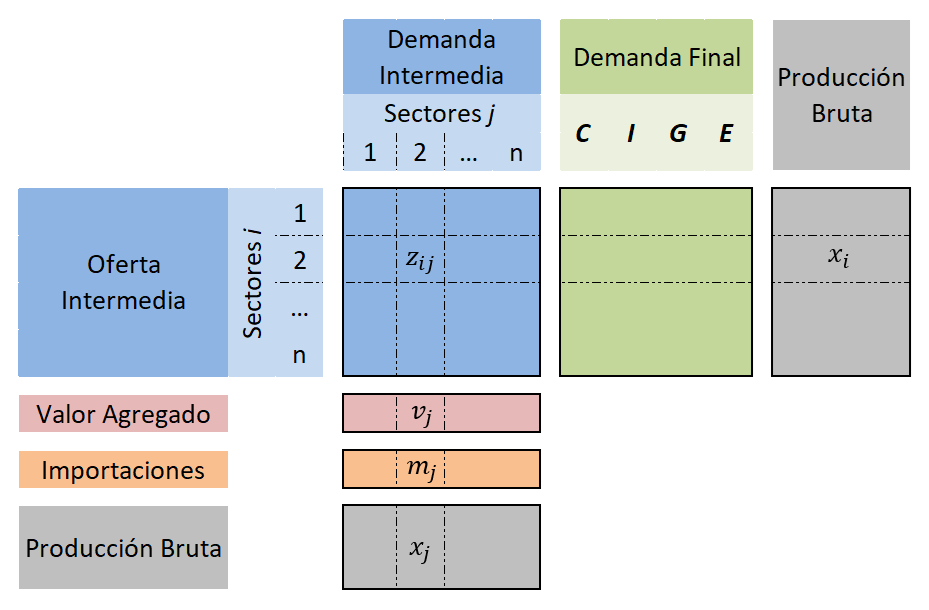
\includegraphics[width=.7\linewidth]{MIP.png}
 \caption{Estructura básica de una \gls{mip} simétrica nacional.}
 \label{Fig_MIP}
\end{figure}

%El modelo insumo--producto es una de las fuentes de información estadística más importantes para estudiar la estructura económica de un país, ya que registra las transacciones que realizan entre sí los sectores económicos resultado de sus demandas y ofertas recíprocas de insumos\parencite{Mariñ11993}
% La elaboración estadística de las MIP se realiza de forma articulada con las cuentas nacionales y existe coherencia entre ambos sistemas. Algunos componentes del sistema de cuentas nacionales coinciden directamente con la MIP \parencite{Mariñ11993} (p-44--46)

\section{Matrices Insumo--Producto Multirregionales}

En las matrices insumo--producto nacionales el comercio internacional es considerado una variable exógena y no se incluye dentro de las relaciones intersectoriales. Las matrices insumo--producto multirregionales o multipaís (\acrshort{mriot})\footnote{Algunos autores usan el término GMRIO (\textit{Global Multiregional Input--Output}) para referirse a estos modelos, como en \textcite{Tukker2013}.} utiliza el marco teórico del modelo de Leontief, pero integran el comercio internacional de bienes y servicios intermedios, reflejando las relaciones intersectoriales entre los países o regiones.  Las fuentes de datos principales de las \gls{mip} multirregionales son las siguientes: a) Las estadísticas de las cuentas nacionales de cada país (cuadros de oferta y utilización o \glspl{mip} nacionales), b) datos sobre el comercio bilateral y, c) datos o supuestos sobre el origen del comercio internacional de los productos intermedios \parencite[p.~17]{Durán2021}.

La figura \ref{Fig_RIOT} muestra de forma simplificada la estructura de una \gls{mriot}. Una \gls{mriot} se compone de una matriz de demanda intermedia $\textbf{Z}_{m+1, m+1}$, donde $m$ es el número de países considerado. Cada elemento de la diagonal de $\textbf{Z}$ es, a su vez, una matriz $\textbf{Z}^{UU}$ de los insumos intermedios domésticos de un país $U$. Los elementos de $\textbf{Z}$ fuera de la diagonal son submatrices $n \times n$ de la forma:
\begin{equation}
 \textbf{Z}^{UV}=\left[\begin{matrix}
  z_{11}^{UV} & \ldots & z_{1n}^{UV} \\
  \vdots & \ddots & \vdots\\
  z_{n1}^{UV}  & \ldots & z_{nn}^{UV} 
 \end{matrix} \right],
\end{equation}
donde cada elemento $z_{ij}^{UV}$ representa los insumos exportados por el sector $i$ del país $U$ e importados por el sector $j$ del país $V$. Estas submatrices representan el flujo de valor en la cadena de valor global \parencite[p.~10]{Xing2022}. Este modelo incluye el comercio entre cada país considerado y todas las economías externas a la región, agrupadas bajo el término \gls{row}.

\begin{figure}[h]
 \centering
 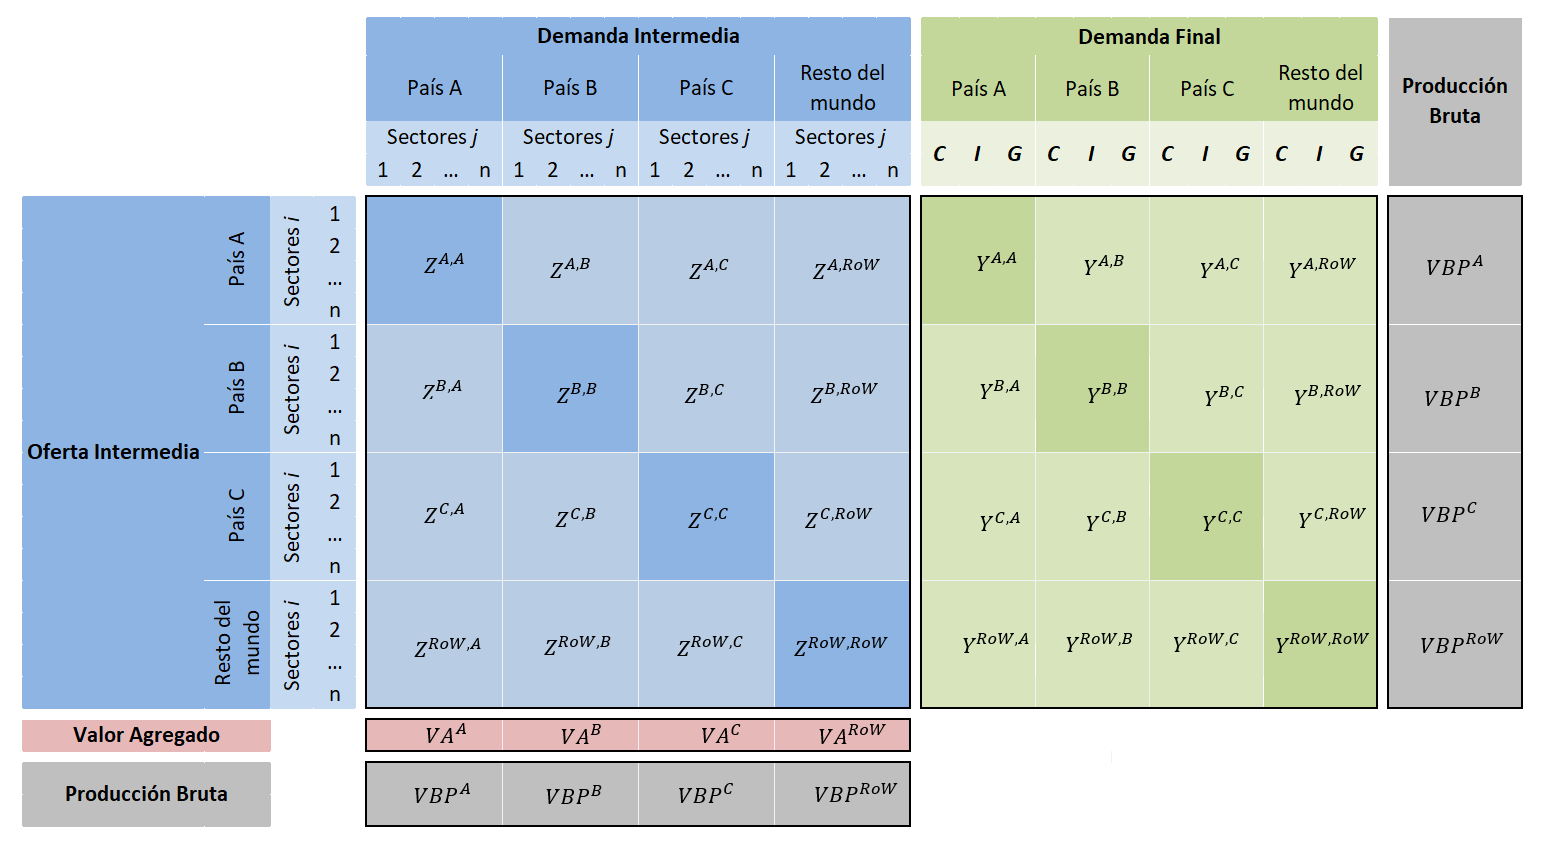
\includegraphics[width=1\linewidth]{MRIOT.png}
 \caption{Estructura básica de una \gls{mriot} de 3 países.}
 \label{Fig_RIOT}
\end{figure}

Para cada país existe un vector fila de valor agregado $\textbf{VA}$ y un vector de producción bruta $\textbf{VBP}$. La demanda final se estructura en una matriz 
\begin{equation}\textbf{Y} = \left[ \textbf{Y}^{UV} \right]\end{equation}
conformada por submatrices $\textbf{Y}^{UV}$ con la información de la producción de cada sector de un país $U$ consumida en el país $V$ \parencite[p.~10]{Xing2022}.

Existe un tipo de matriz intermedia, denominada \gls{riot}. La \gls{riot} generalmente se concentra en una región del mundo y no incluye información sobre el consumo intermedio que es exportado por la región al resto del mundo, el consumo intermedio extrarregional ni la demanda final que es importada de fuera de la región. Se trata de una \gls{mriot} incompleta, que no está cerrada con el mundo \parencite[p.~19]{Durán2021}.

Las principales matrices insumo--producto multirregionales son:
\begin{itemize}
 \item \textit{Inter--Country Input--Output Tables} (\acrshort{icio}). Es una \gls{mriot} elaborada por la \gls{ocde}. Su última versión de 2025 muestra el flujo de bienes y servicios finales e intermedios de 80 países\footnote{Incluyen los 38 países de la  \gls{ocde}, y todos los países dentro del G20 y la \gls{ue}.} más el resto del mundo y 50 sectores, para el periodo 1995--2022. Los sectores se clasifican de acuerdo con la revisión 4 de la \gls{isic}. La versión extendida divide las economías de China y México en dos (mercado nacional y exportador).  Además del consumo intermedio, las tablas incluyen seis categorías de demanda final por país,\footnote{Gasto en consumo final de hogares; instituciones sin fines de lucro al servicio de los hogares; consumo final del gobierno general; formación bruta de capital fijo; cambios en inventarios y objetos de valor; y compras directas en el exterior por parte de residentes.} el valor agregado, y los impuestos menos subsidios a productos intermedios y finales por cada par país--industria \parencite{OECD-ICIO}.
 
 Existen varias versiones anteriores de esta base de datos. La versión de 1995 cubre 10 países de la \gls{ocde} y 35 industrias (\gls{isic} Rev. 2) durante el periodo de 1968 a 1990. La segunda versión de 2002 aumentó el número de países a 20 y de sectores a 42, con datos de 1992 a 1997. Mientras que la versión de 2006 incluía 37 países, 28 sectores y se amplió el periodo de análisis al año 2000 \parencite{Yamano2006}. En ambos casos la clasificación corresponde a la revisión 3 de la \gls{isic}. La edición de 2021 incluía datos de 71 países y 45 industrias para el periodo 1995--2018; mientras que la versión 2023 agregó 4 países más.
 
 Para su construcción, la \gls{ocde} utiliza tablas insumo--producto, y en su defecto, tablas de oferta y utilización generadas por los institutos nacionales de estadística. Los datos son armonizados en cuatro sentidos: homogeneizar los datos provenientes de diferentes países en la clasificación industrial de la \gls{isic}; estructurar los datos como una matriz industria--industria; expresar los valores en precios básicos;\footnote{Un precio básico es la cantidad de dinero que cobrará el productor al comprador por cada unidad de un bien o servicio producido menos los impuestos por pagar más las subvenciones por cobrar por el productor. Esto no incluye los gastos del transporte que el productor facture por separado \parencite[p.~8]{CEPAL2013}. No debe confundirse el término con los precios constantes a un año base.} y ajustarse con las estimaciones de los Sistemas de Cuentas Nacionales de cada país. Para más detalles metodológicos del proceso de armonización, véase \textcite{Yamano2006}.
 
 \item \textit{World Input--Output Database} (\acrshort{wiod}). Esta base de datos contiene los valores de transacciones anuales intersectoriales entre 43 países\footnote{28 países de la \gls{ue}, otros 15 países importantes del mundo y estimaciones sobre el resto del mundo en conjunto} y 56 sectores de acuerdo con \gls{isic} revisión 4, para el periodo 2000--2014, así como los flujos de cada industria--país a hogares, gobierno y usuarios de bienes de capital. Los valores de las tablas están expresados en precios de producción (o básicos) corrientes, en millones de dólares estadounidenses \parencite{Timmer2015}. %Uno of the objectives of WIOD is to permit the histórica comparison of the production, the agregated value and the commercial flujos in the economic environment }.
 Las tablas de insumo--producto mundial (\textit{World Input--Output Tables}, \acrshort{wiot}), núcleo de la WIOD, se construyeron a partir de series de tiempo de los cuadros de oferta y utilización (\textit{Supply and Use Tables}, \acrshort{sut}) nacionales, datos de las cuentas nacionales y estadísticas de comercio internacional. Los cuadros de oferta y utilización nacionales son utilizados como base para la construcción de una \acrshort{sut} mundial, la cual es transformada posteriormente en una \acrshort{wiot} \parencite{Dietzenbacher2013}. 
 
 Existe una versión de 2013, la cual cubre 35 industrias y 40 países para el periodo 1995--2011 y una versión de largo plazo que contempla el periodo de 1965--2000 con 25 países y 23 sectores económicos. En ambos la clasificación corresponde a la \gls{isic} revisión 3. El proyecto fue desarrollado por un equipo de la Universidad de Groningen, en Países Bajos y fue financiado por la \gls{ec} y la \acrlong{nwo}, \acrshort{nwo} \parencite{WIOD}.
 
 \item \textit{The Global Trade Analysis  Project} (\acrshort{gtap}) es una base de datos de paga que contiene tablas de insumo--producto nacionales, comercio bilateral y datos energéticos y ecológicos, de 141 países y 65 sectores, utilizando 5 años de referencia (2004, 2007, 2011, 2014, 2017) en su última versión de 2023 \parencite{GTAP11}. En total hay 11 versiones de la base de datos, que cubren el periodo entre 1993 y 2023, las cuales fueron agregando progresivamente países y sectores \parencite{GTAP_History}. Aunque la base \acrshort{gtap} no incluye directamente la matriz del comercio entre todos los países, puede construirse directamente una \gls{mriot} sin necesidad de hacer cálculos de equilibrio, como muestran en \textcite{Koopman2010, Peters2011, Andrew2013}. Esta base de datos no fue pensada para ofrecer tablas IO, sino para facilitar la simulación económica, asegurando que los datos económicos sean consistentes \parencite{Peters2011, Wiedmann2011}. Debido a que la base \acrshort{gtap} solo se compara con las estadísticas comerciales, los datos de oferta y demanda a nivel sectorial para países individuales pueden tener grandes discrepancias con los datos de las cuentas nacionales correspondientes. Este proyecto fue desarrollado por el Centro de Análisis del Comercio de la Universidad de Purdue \parencite{Jones2014}.
 
 \item \textit{International Input--Output Tables} del \gls{ide-jetro}. Esta base de datos está compuesta de tres \gls{mip} multirregionales:
 \begin{itemize}
  \item \textit{Asian International Input--Output Table} (AIIOT), 2005. Es una \gls{mriot} de 9 países asiáticos y los Estados Unidos y 76 sectores económicos. Considera otros elementos como importaciones y exportaciones a otros países específicos y al resto del mundo, valor agregado, demanda final y discrepancias estadísticas. Existen versiones anteriores de esta tabla, para los años 1985, 1990, 1995 y 2000.
  \item \textit{Transnational Interregional Input--Output Table for China, Japan and Korea} (TIIOT-CJK), 2005. La tabla están conformadas por los flujos insumo--producto entre 20 regiones de China, Japón y Corea del Sur, junto con las economías nacionales de Taiwán, los Estados Unidos, Hong Kong, y la economía agregada de los países de la \acrfull{asean} y el resto del mundo. En cuanto a las industrias, la tabla incluye dos clasificaciones, con 10 y 15 sectores agregados, respectivamente. Además, se reportan otros elementos en la tabla, como subdivisiones del valor agregado y la demanda final, costo de fletes, impuestos a importaciones y discrepancias estadísticas.
  \item \textit{BRICs International Input--Output Table 2005}. Esta tabla incluye los flujos insumo--producto de cada país de los BRICS\footnote{Foro político y económico formado por Brasil, Rusia, India, China y Sudáfrica (hasta 2023).} (excepto Sudáfrica), Japón, los Estados Unidos y la economía agregada de los países de la \acrlong{ue}, así como las importaciones y exportaciones al resto del mundo. Presenta dos clasificaciones de industrias en 7 y 25 sectores agregados \parencite{Meng2013, IDE-JETRO}.
 \end{itemize}
 Estas bases de datos reportan precios corrientes del productor, en miles de dólares estadounidenses. Una de sus desventajas es que sus datos solo corresponden a años de referencia específicos, a precios corrientes, por lo cual no pueden utilizarse en análisis a lo largo del tiempo \parencite[p.~578]{Timmer2015}.
 
 \item \textit{The Eora Global Supply Chain Database}. Es una base de datos de paga,\footnote{La base fue creada y es mantenida principalmente por investigadores de la Escuela de Física de la Universidad de Sydney, Austrialia, bajo financiamiento del \gls{arc} \cite[p.~103]{Miller2022}.} que proporciona una serie temporal de tablas insumo--producto, a precios corrientes, con cuentas satélite sociales y ambientales correspondientes a 192 economías y entre 26 y 511 sectores dependiendo del país.  La diferencia entre sectores se debe a que intentan mantener la clasificación sectorial de cada país cuando sea posible. La base de datos contiene series históricas de 1990 a 2022. Dado que considera prácticamente a todos los países del mundo, no construyen un agregado para el ``resto del mundo''. Existe una versión simplificada, denominada \textit{EORA26}, donde se usa una clasificación común de 26 sectores para todos los países, y las tablas de oferta y utilización del modelo completo se transforman en tablas de oferta y utilización simétricas producto--producto e industria--industria. Este modelo simplificado es más fácil de usar, pero menos preciso \parencite{EORA}. 

 Para su construcción combinan información de cuadros de oferta y utilización, así como tablas industria--industria y mercancía--mercancía de distintos países. La obtención de la \gls{mip} multirregional se realiza mediante estimaciones y el uso de métodos de optimización para asegurar el equilibrio de las tablas, a la vez que se intenta evitar la transformación de los datos originales de cada país, en aras de la transparencia
 \parencite{Lenzen2012, Lenzen2013}.
 

El objetivo del equipo que desarrolló este proyecto fue alcanzar el mayor grado de detalle respecto a los países, sectores y número de años. Además de las tablas de oferta y consumo y de insumo--producto, la base de datos \textit{Eora} tiene extensiones que incluyen consumo de energía, emisiones de gases de efecto invernadero y otras variables ambientales \parencite{Wiedmann2011}. Aunque sus datos cubren prácticamente a todas las economías del mundo, dependen de métodos de imputación para llenar los datos faltantes en países con sistemas estadísticos poco desarrollados \parencite[p.~579]{Timmer2015}.% Las tablas son presentadas en precios básicos.
 
 \item \textit{Asian Development Bank Multiregional Input--Output Tables} (\acrshort{adb}--MRIO) es una \gls{mip} multirregional elaborada por el \gls{adb} a partir de los datos de \gls{wiod}. Incluye 62 economías, más el resto del mundo, con desagregación por 35 industrias y 5 categorías de demanda final a precios constantes (base 2010). Estas tablas cubren el periodo de 2007 a 2023 y el año 2000. El \acrshort{adb}--MRIO también incluye tablas a precios corrientes para los mismos años, y para el periodo de 2017 a 2023 además incluye tablas con 72 economías \parencite{ABD}.
 
 \item \textit{Externality Data and Input--Output Tools for Policy Analysis} (EXIPOL). Es una \gls{riot} europea que cubre 27 países de la Unión Europea y otros 16 países (más el resto del mundo), así como 129 sectores industriales y productos. El objetivo principal del proyecto EXIPOL es mejorar la comprensión de los costos externos de las presiones ambientales. La tabla incluye información sobre el país de origen de cada producto y el sector receptor del país importador \parencite{Tukker2009, Wiedmann2011, Tukker2013}.
 
 \item Tablas regionales de insumo--producto de la zona euro:
 \begin{itemize}
  \item \textit{European Multi Regional Input Output}. Es una matriz insumo--producto regional de la Unión Europea, que incluye los flujos comerciales entre 272 regiones europeas (\acrshort{nuts}-2)\footnote{La \gls{nuts} es una clasificación jerárquica de 3 niveles, elaborada por la \gls{eurostat} para dividir geográficamente los países de la Unión Europea en regiones y subregiones para fines estadísticos y presupuestales. La \gls{nuts}-2 corresponde a regiones que tienen un rango poblacional entre 800 mil y 3 millones de habitantes \parencite{NUTS}.} y 10 sectores para el periodo 2008--2018 \parencite{Huang2023}.
  \item \textit{Eurostat's FIGARO\footnote{\textit{Full International and Global Accounts for Research in Input-Output Analysis}.} input--output tables}. Es una base de datos creada por la \gls{eurostat}, que incluye tablas de insumo--producto regional para 45 países (27 de la \gls{ue}), más el resto del mundo, y 64 industrias, para los años 2010--2022, así como componentes de la demanda final y el valor agregado \parencite{FIGARO}.
  
  %\item EUREGIO: The Construction of a Global IO Database With Regional Detail for Europe for 2000–2010. https://papers.ssrn.com/sol3/papers.cfm?abstract_id=3285818
 \end{itemize}
\end{itemize}

En la tabla \ref{tab_MRIOT} se comparan las características de las últimas versiones de cada \gls{mriot}. Se muestra el nombre de la base de datos y el año o número de su última versión. La tercera columna indica el número de países cubierto, mientras que la cuarta columna representa el número de sectores o industrias que incluye la base de datos. La quinta columna contiene el número de componentes de la demanda final que son considerados en la \gls{mriot}, mientras que la última columna muestra los años disponibles.


\begin{table}[h]
\centering
\caption{Características de las principales matrices insumo--producto multirregionales.}
\label{tab_MRIOT}
\begin{tabular}{@{} p{4cm} c c c p{2cm} p{2cm} @{}} 
\hline
\textbf{Base de datos} & \multicolumn{1}{l}{\textbf{Versión}} & \multicolumn{1}{l}{\textbf{Economías}} & \multicolumn{1}{l}{\textbf{Sectores}} & \textbf{Demanda final} & \textbf{Periodo} \\ \hline
OECD--ICIO & 2025 & 81 & 50 & 6 & 1995--2022 \\
WIOD & 2016 & 43 & 56 & 5 & 2000--2014 \\
GTAP & v11 & 141 & 65 & -- & 2004, 2007, 2011, 2014, 2017 \\
AIIOT & 2005 & 10 & 76 & 5 & 2005 \\
IDE--JETRO (BRICS) & 2005 & 7 & 10, 15 & 5 & 2005 \\
TIIOT-CJK & 2005 & 7 & 10, 15 & 5 & 2005 \\
EORA & v199.82 & 190 & 26--511 & 6 & 1990--2022 \\
ABD--MRIO & 2023 & 62 & 35 & 5 & 2000, 2007--2023 \\
EXIPOL & -- & 43 & 129 & -- & -- \\
European MRIO &  2023 & 27 & 10 &  5 &  2008--2018\\
FIGARO & -- & 45 & 64 & 4 & 2010--2022 \\ \hline
\end{tabular}
\end{table}
% TIIOT-CJK - 20 regiones
% EUROPEAN MRIO 272 regiones


La necesidad de armonizar y consolidar datos de diferentes sistemas estadísticos nacionales ha dificultado que los institutos nacionales de estadística y organismos supranacionales contribuyan en la construcción de \gls{mip} multirregionales, con la excepción de la base de datos de la \gls{ocde} \parencite[p.~7]{Tukker2013}. 

En \textcite{Jones2014} comparan tres \gls{mip} multirregionales (\gls{wiod}--2013, \acrshort{icio} versión 2013 y \acrshort{gtap} v8) con los datos de estadísticas oficiales para el periodo 2004--2009. Después de armonizar las tres tablas en la misma clasificación de países y sectores, verifican su coherencia con estadísticas oficiales de las \gls{unna}: \gls{pib} de cada país (basado en cuenta de gastos), demanda interna final y balanza de pagos. Los autores encontraron que los valores del \gls{pib} y de la demanda final calculados a partir de los datos de las tablas \gls{icio} son consistentes con los datos informados por la UNNA, presentando pequeñas desviaciones. Por su parte, los cálculos de ambos indicadores basados en \gls{wiod} fluctúan alrededor de los valores de referencia de las \gls{unna} ($\pm 1\%$ para el 70\% de las economías consideradas). Mientras que la base \gls{gtap} presenta valores consistentemente inferiores a los informados por las \gls{unna}, con diferencias significativas para algunos países. Las diferencias entre las estadísticas oficiales y las tres MIP multirregionales son mucho mayores y fluctúan más en los valores comerciales (importaciones y exportaciones) que en términos del \gls{pib} o la demanda final. Las tablas \gls{icio} son las que presentan las menores diferencias con los datos oficiales: para la mayoría de las economías no pertenecientes a la \gls{ue}, presentan diferencias negativas pequeñas o insignificantes, mientras que las mayores diferencias se presentan en países miembros de la \gls{ue}. Los datos basados en \gls{wiod} son consistentemente menores que las estadísticas oficiales, particularmente en países de la \gls{ue}. Los autores sugieren que estas desviaciones pueden deberse, en gran parte, al registro sobre reexportaciones y comercio de tránsito que tiene lugar dentro de la \gls{ue}.

En esta tesis se decidió trabajar con las tablas \gls{icio} versión 2025 por las siguientes razones. En primer lugar, por su amplia cobertura en términos de países, sectores y años. En segundo lugar, por su metodología armonizada con los sistemas de cuentas nacionales y las matrices insumo--producto oficiales de cada país, así como con la clasificación internacional de la \gls{isic} revisión 4. Además, sus datos son consistentes con las estimaciones del \gls{pib}, la demanda final y la balanza de pagos de los países. %de acuerdo con el trabajo de \parencite{Jones2014}. 
Finalmente, es una base de datos abierta y gratuita, elaborada por un organismo supranacional.

En la tabla \ref{Tab_Cobertura_PorContinente} se presenta el número de países considerados  en la base de datos \gls{icio}--\gls{ocde} versión 2025, agrupados por continente. Por su parte, la figura \ref{Fig_Cobertura_ICIO25} muestra en rojo los países cubiertos por esta base de datos, mientras que los países no resaltados son agrupados bajo la categoría ``resto del mundo''. Las tablas \ref{ICIO25_Paises} y \ref{ICIO25_Industrias} del anexo \ref{anexo1} muestran el listado detallado de los países y sectores incluidos en la base. 

\begin{table}[H]
	\centering
	\caption{Cobertura por continente de la base ICIO--OCDE versión 2025}
	\label{Tab_Cobertura_PorContinente}
	\begin{tabular}{lr}
		\toprule
		\textbf{Continente} & \textbf{Cantidad} \\ \midrule
		Europa              & 33                                    \\
		Asia                & 25                                    \\
		África              & 11                                    \\
		Sudamérica          & 5                                     \\
		América del Norte   & 4                                     \\
		Oceanía             & 2                                     \\ \bottomrule
	\end{tabular}	
\end{table}

\begin{figure}[H]
 \centering
 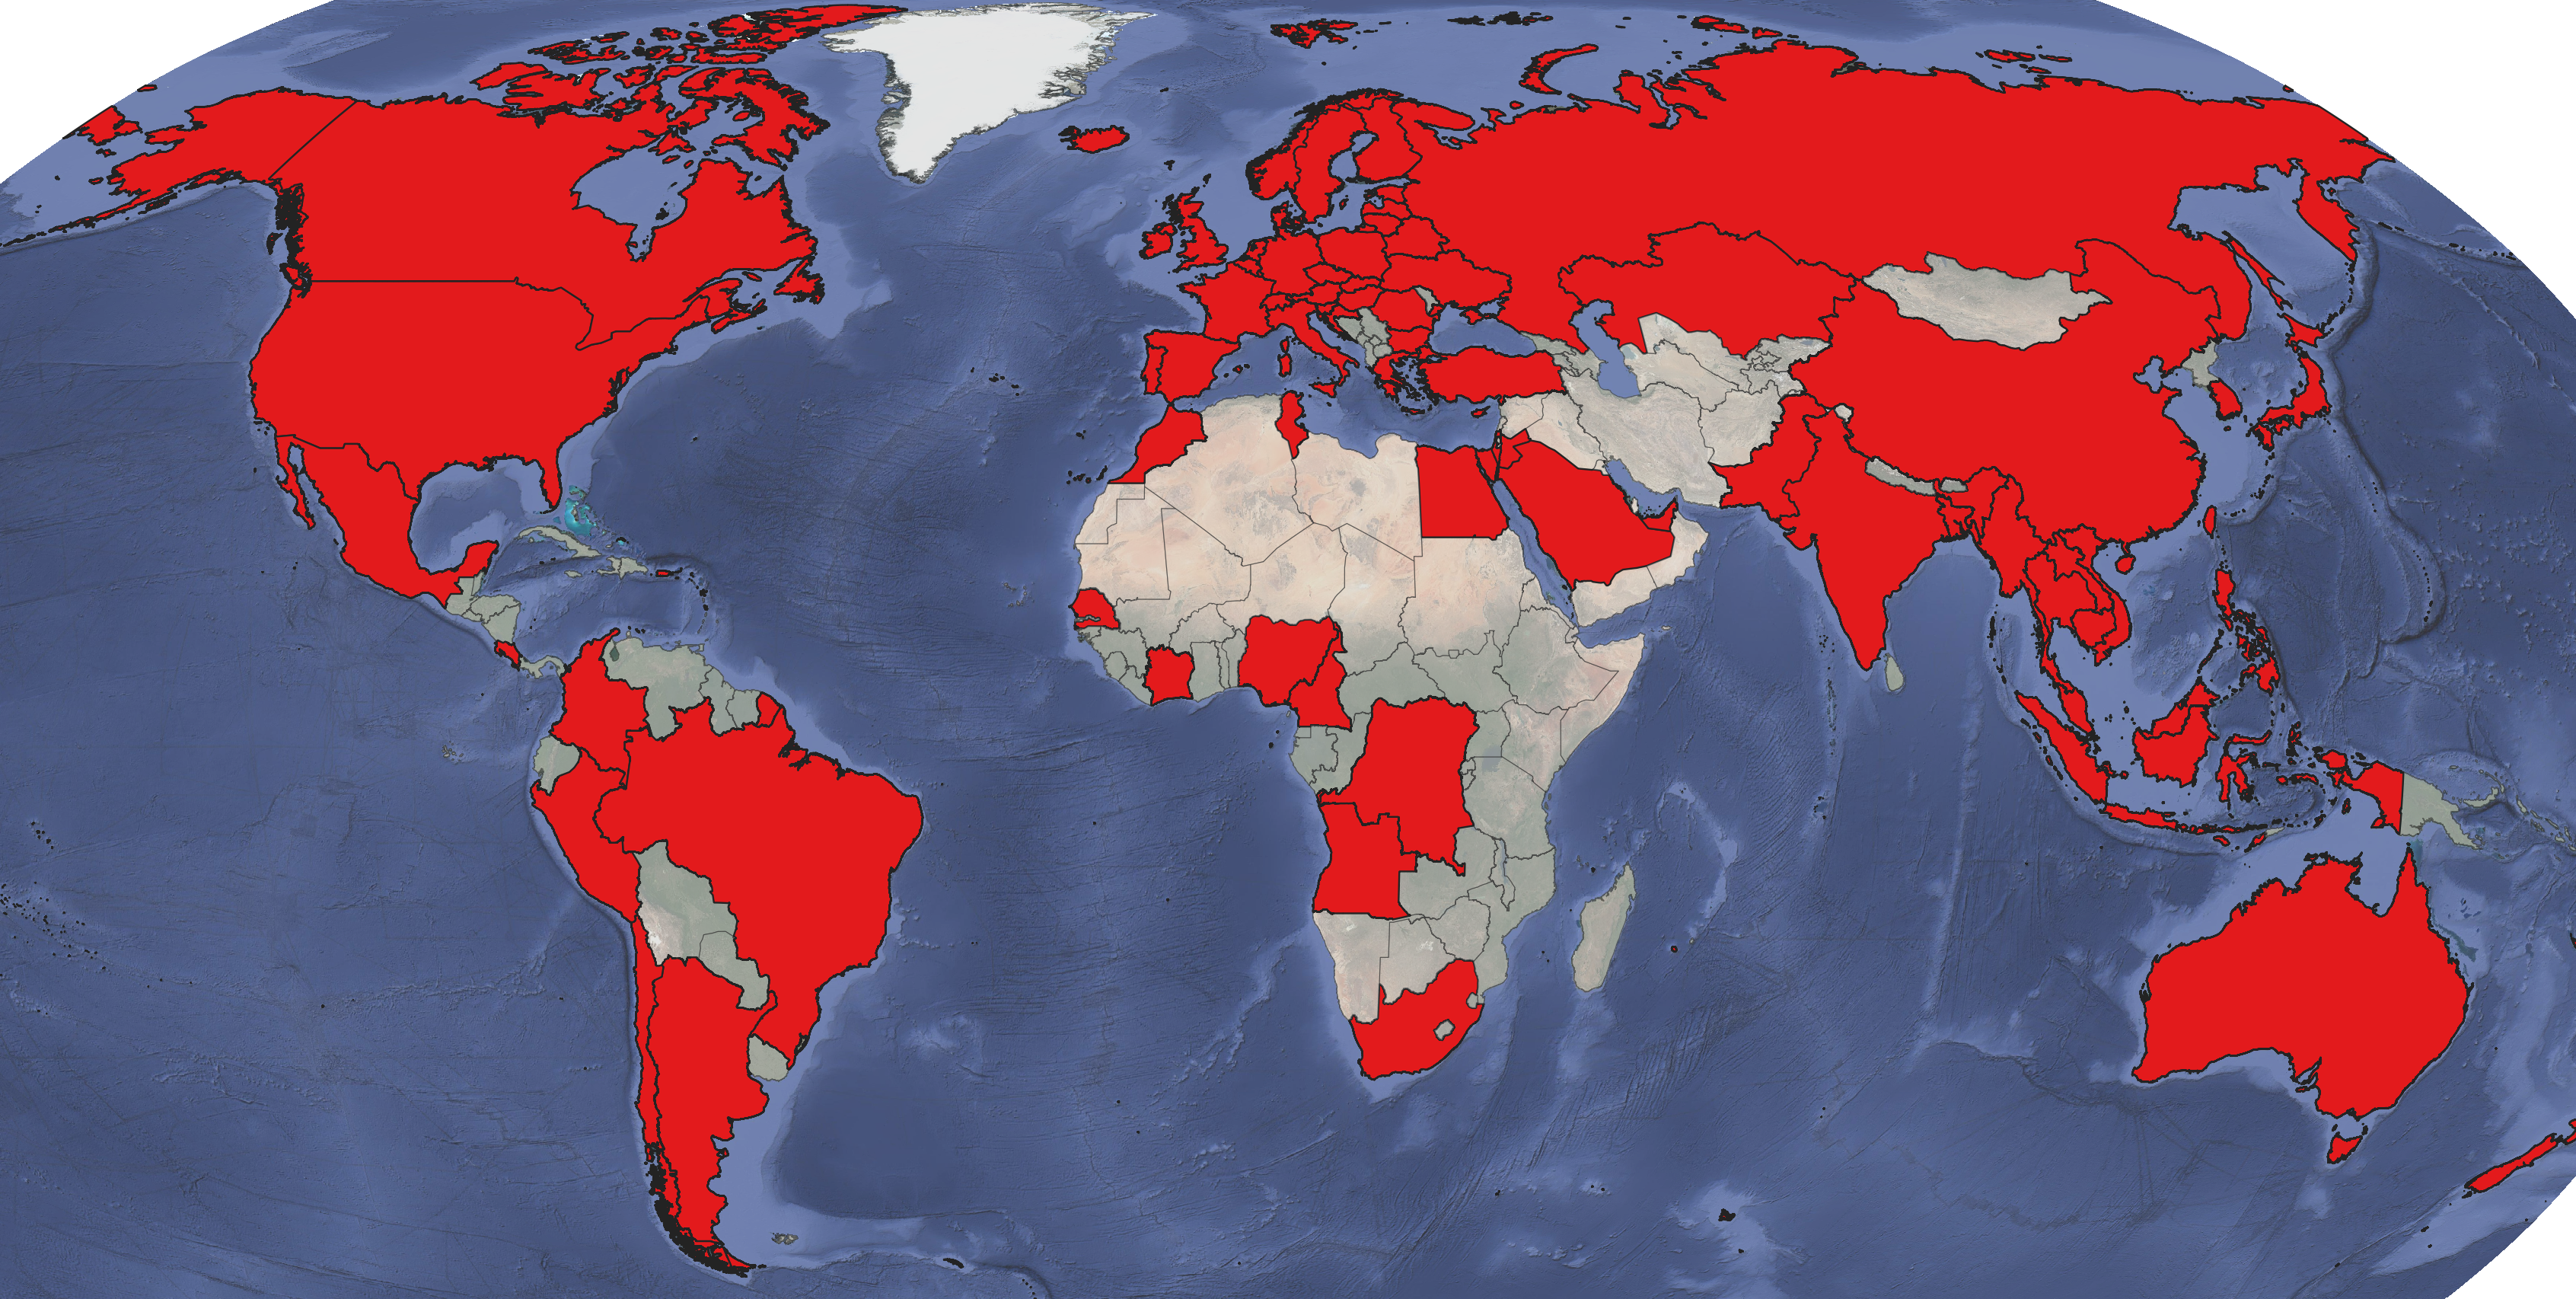
\includegraphics[width=\linewidth]{Cobertura2025.png}
 \caption{Cobertura geográfica de la base ICIO--OCDE versión 2025.}
 \label{Fig_Cobertura_ICIO25}
\end{figure}



%\textcolor{red}{[Agregar mapa de países considerados y tabla de sectores.]}





	\chapter{Redes de insumo-producto}

\section{Construcción de la red de insumo-producto internacional}

Los datos de las matrices insumo-producto multirregionales han demostrado ser una herramienta confiable para analizar la globalización económica. Gracias a ellos, se puede estudiar las cadenas globales de valor y estudiar de manera simultánea las interrelaciones en las economías nacionales y regionales \parencite[p.~18]{Xing2022}. Una forma de realizar este estudio es representar la información del modelo de insumo producto como una red y utilizar los métodos de la teoría de redes. 

A partir de la submatriz de consumo intermedio de una \acrfull{mriot} es posible establecer una red del flujo comercial interindustrial internacional. Cada sector de cada país  es representado por un vértice de un grafo, y se establece una arista entre dos vértices si existe flujo comercial entre sus correspondientes sectores. Debido a que el flujo comercial tiene una dirección, del sector vendedor al sector comprador, la arista puede considerarse como dirigida. El valor del flujo comercial de un sector a otro se asocia a su respectiva arista. De esta manera, la interdependencia del sistema económico internacional es modelada como un grafo dirigido y ponderado.

Matemáticamente, un grafo $G$ se define formalmente como un par ordenado $(V,E)$ donde $V$ es un conjunto de vértices y $E$ un conjunto de aristas. El número de vértices $n=|V|$ es denominado el orden del grafo y el número de aristas $m=|E|$ su tamaño \parencite[p.~2]{Bondy2008}. Dos vértices son adyacentes si están conectados por una arista; y una arista que tiene como extremo a un vértice se dice que es incidente a éste. El número de aristas incidentes a un vértice se denomina el grado del vértice. Un grafo puede ser representado por su matriz de adyacencia $A(G) = [a_{ij}]$, donde $a_{ij}=1$ si existe una arista $(i,j)\in E$ y $0$ en caso contrario. Las aristas dirigidas son conocidas como arcos, y al grafo que las contiene como digráfica o grafo dirigido. Un arco es un par ordenado de vértices $e=(i,j), \ i,j\in V$ donde el primer vértice $i$ indica el punto de inicio, y el segundo vértice $j$ es el punto de llegada \parencite[p.~31] {Bondy2008}. Cuando el grafo representa un sistema se denomina red \parencite[p.~7]{Estrada2012}. Un grafo o una red es ponderada, si se asocia un número real o peso $w(e)$ a cada arista $e\in E$, y es denotada con $G=(V,E,w)$ \parencite[p.~50]{Bondy2008}. 

Para construir el conjunto de redes insumo-producto internacional basadas en las tablas \gls{icio} se siguió el siguiente procedimiento:
\begin{itemize}
    \item Para cada tabla anual \gls{icio}, se consideró la submatriz cuadrada de demanda intermedia $\textbf{Z}(t)=\left[z_{ij}^t \right]$, donde $z_{ij}^t$ es el valor de los bienes y servicios que un sector-país $i$ vende al sector-país $j$ en el año $t$, a precios corrientes y del productor, en dólares estadounidenses.\footnote{Debido a su alto nivel de agregación, no se consideraron los datos agrupados como ``resto del mundo'' (\gls{row}).} Todas las submatrices tienen $n=80*50$.
    \item Para cada año se calculó el flujo  intermedio total $tot(t)$, entendido como el valor total de los intercambios comerciales entre todos los sectores de todos los países considerados en el año $t$. Esta cantidad es igual a la suma de los totales por filas o por columnas\footnote{Observe que el sistema no es cerrado, ya se ha descartado la información del valor agregado y de la demanda final. Por lo tanto, la suma de una fila $i$  no necesariamente coincide con la suma de la columna $i$.}:
    \begin{equation}
    	tot(t) = \sum_{j=1}^{n} \left(\sum_{i=1}^{n} z_{ij}^t\right)= \sum_{i=1}^{n} \left(\sum_{j=1}^{n} z_{ij}^t\right) 
    \end{equation}
    \item Después, se calcula la matriz de proporciones interindustriales
	 \begin{equation}
	 	\textbf{Z}^{'}(t) = \left[\frac{z^t_{ij}}{tot(t)}\right] = \left[ x^t_{ij}\right]
	 \end{equation}
    dividiendo cada elemento de $\textbf{Z}(t)$ entre $tot(t)$. Los elementos de esta matriz
    son la proporción de cada flujo interindustrial respecto al total del comercio intermedio de un año específico. De esta forma, se pueden hacer comparaciones históricas sin verse afectadas por las diferencias anuales en los precios corrientes.
    \item Para cada año se construyó una red \gls{icio} $G^{t}=(V^{t}, E^{t}, w^{t})$, tal que:
    \begin{itemize}
        \item El conjunto de vértices $V^{t}$ está constituido por todas las combinaciones de países y sectores económicos, con un total de $n=4,000$ vértices en cada grafo.
        \item Se establece un arco en $E^{t}$ entre dos vértices $i,j\in V^t$ (incluyendo $i=j$) si su correspondiente proporción en $\textbf{Z}^{'}(t)$ es positiva, es decir, si $x^t_{ij}>0$. %No se consideraron los lazos, es decir, las aristas $e=(i,i), \ i\in V$.
        \item La función de pesos $w^t : E^t \rightarrow (0,1)$
        se define como
     	\begin{equation}
        	w^t(i,j) := x^t_{ij}
     	\end{equation}
    \end{itemize} 
\end{itemize}

%En la figura \ref{Fig_RedIcio} se ilustra el proceso de construcción para un modelo con 3 países y 3 sectores.

%\begin{figure}[H]
%\centering
%\begin{subfigure}{.32\textwidth}
  %  \includegraphics[width=\textwidth]{A.png}
%    \caption{\footnotesize{MRIOT\\ $ $}}
%\end{subfigure}
%\begin{subfigure}{.32\textwidth}
  %  \includegraphics[width=\textwidth]{B.png}
%    \caption{\footnotesize{Matriz de proporciones\\interindustriales}}
%\end{subfigure}
%\begin{subfigure}{.32\textwidth}
%    \includegraphics[width=\textwidth]{C.png}
%    \caption{\footnotesize{Red de insumo-producto\\ internacional}}
%\end{subfigure}
%\label{Fig_RedIcio}
%\end{figure}

%Los otros elementos del modelo insumo producto, es decir, los datos de la demanda final y el valor agregado también pueden integrarse en un enfoque basado en redes. En este modelo está formado por tres capas. La primera es formada por vértices que corresponden a los elementos del valor agregado de cada país-sector, y con aristas que apuntan a los vértices de la matriz de uso intermedio.  % Noción de multicapas Xing (2022) p. 19. 

\section{Detección de comunidades}

La detección de comunidades es un problema de la teoría de redes que consiste en buscar una división de los vértices de una red en grupos o comunidades, de tal forma que los vértices dentro de cada comunidad estén densamente conectados entre sí, mientras que los vértices que pertenecen a distintas comunidades estén escasamente conectados \parencite[p.~2]{Blondel2008}.  Las definiciones tradicionales de comunidad comparan la proporción de aristas dentro y entre las comunidades. Sin embargo, el punto de vista moderno se enfoca en la probabilidad de que un vértice comparta aristas con un subgrafo. La existencia de comunidades implica que los vértices interactúan con mayor intensidad con otros miembros de su comunidad, que con los vértices de otras comunidades \parencite[p.~7]{Fortunato2016}.

La función más utilizada para medir la calidad de una partición de los vértices en comunidades es la modularidad \parencite[p.~29]{Fortunato2016},  definida por   \textcite{Newman2004}. Dada una $k$-partición\footnote{Una $k$-partición de un conjunto $V$ se define como una colección de conjuntos $$P=\{C_1, C_2, \ldots, C_k\}$$ que satisface tres condiciones:
	\begin{enumerate}
		\item La unión de todas las partes es igual al todo $$\bigcup_{C_i\in P}C_i=V$$
		\item Las partes son disjuntas por pares $$C_i \cap C_j =\emptyset, \quad \forall C_i,C_j\in P, \ i\neq j$$
		\item No hay partes vacías $$C\neq \emptyset, \quad \forall C_i\in P$$
\end{enumerate}} $P=\{C_1,C_2,\ldots,C_k\}$ de $V$, la modularidad se define como
\begin{equation}
    Q(P) = \frac{1}{2m}\sum_{i,j\in V} \left(a_{ij}-p_{ij}\right) \delta(C_i,C_j) \label{C3_eq_modularity_general}
\end{equation}
donde $a_{ij}$ son los términos de la matriz de adyacencia de $G$; $p_{ij}$ representa el valor esperado de conexión entre los vértices $i$ y $j$, si las conexiones de la red se reconectaran de forma aleatoria, pero respetando ciertas propiedades de la red original; y $\delta(C_i, C_j)$ es una función que es igual a 1 si los vértices $i$ y $j$ pertenecen a la misma partición y 0 en caso contrario, conocida como delta de Kronecker. La elección estándar es suponer que la red aleatoria de comparación (\textit{modelo nulo}) preserva en promedio el grado de todos los vértices. Bajo este supuesto,  la probabilidad de que los vértices $i$ y $j$ con grados $k_i$ y $k_j$ es igual a $\frac{k_i}{2m}$ y $\frac{k_j}{2m}$ respectivamente, por lo tanto, el número de conexiones esperados entre $i$ y $j$ es igual a \parencite[p.~29]{Fortunato2016}:
\begin{equation}
	p_{ij} = 2mp_ip_j = \frac{k_ik_j}{2m}
\end{equation}

Sustituyendo el término $p_{ij}$ en \eqref{C3_eq_modularity_general} se llega a la formulación clásica de la modularidad:
\begin{equation}
	Q(P) = \frac{1}{2m}\sum_{i,j\in V} \left(a_{ij}-\frac{k_ik_j}{2m}\right) \delta(C_i,C_j) \label{C3_eq_modularity1}
\end{equation}

%El término $\frac{k_i}{2m}\frac{k_j}{2m}=p_ip_j$ puede interpretarse como el número de aristas esperados entre $i$ y $j$, si las aristas de la red fueran reconectadas de manera aleatoria, pero conservando en promedio el grado de todos los vértices . 

Debido a que la delta de Kronecker sólo contribuye para los pares de vértices que pertenecen al mismo grupo, la suma puede agruparse por clúster y reformularse\footnote{Los pasos detallados de esta reformulación pueden encontrarse en la sección 9.11 de \textcite{Barabasi}.} de la siguiente manera
\begin{equation}
Q(P) = \sum_{C\in P} \left[\frac{l_C}{m}-\left( \frac{k_C}{2m}\right)^2 \right] \label{C3_eq_modularity2}
\end{equation}
donde $l_C$ es el número total de aristas que unen vértices de la comunidad $C$ y que $k_C$ es la suma de los grados de los vértices que pertenecen a la comunidad $C$. El primer término de cada sumando de la ecuación \ref{C3_eq_modularity2} es la fracción de aristas del grafo que están dentro de la comunidad $C$, mientras el segundo término es la fracción de aristas esperadas en la comunidad $C$ si el grafo se conectara de manera aleatoria, preservando los grados de los vértices en promedio \parencite[p.~29]{Fortunato2016}. 

El valor de la modularidad $Q(P)$ se encuentra acotada dentro del rango $[-1,1]$. Si la proporción de aristas dentro de las comunidades es igual o peor que las esperadas en el modelo aleatorio se obtienen valores de  $Q(P)$ cercanos a 0 o negativos; mientras que una modularidad igual a 1, indicaría una estructura comunitaria muy fuerte; aunque en la práctica, la modularidad en redes con comunidades reales suele toma valores entre  0.3  y 0.7 \parencite[p.~7]{Newman2004}. La figura \ref{Fig_ModularidadEjemplo} muestra un comparación entre la modularidad de una partición que refleja la estructura comunitaria de la red y la modularidad de una partición aleatoria.


\begin{figure}[H]
\centering
\begin{subfigure}{.45\textwidth}
	\centering
  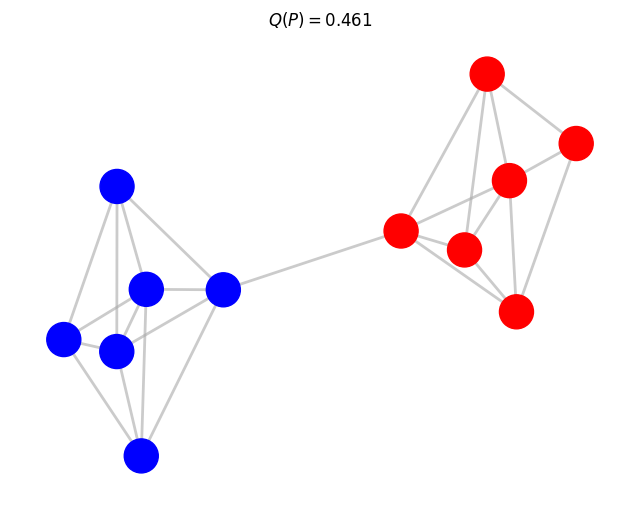
\includegraphics[width=\textwidth]{Modularidad1.png}
\end{subfigure}
\hfill
\begin{subfigure}{.45\textwidth}
	\centering
  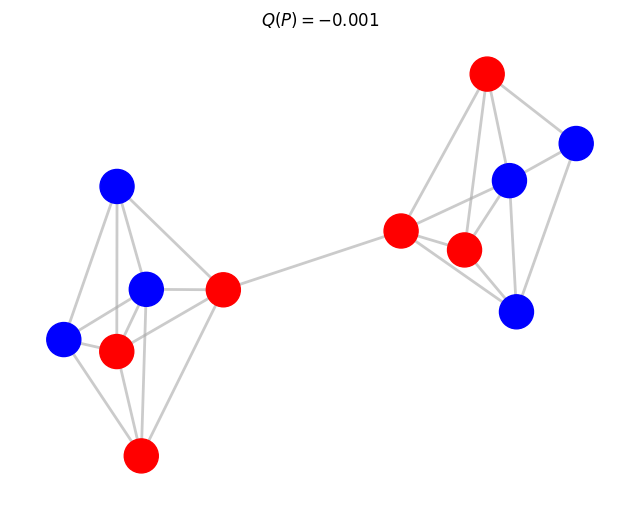
\includegraphics[width=\textwidth]{Modularidad2.png}
\end{subfigure}
    \caption{Modularidad de dos particiones de una misma red.}
    \label{Fig_ModularidadEjemplo}
\end{figure}

La modularidad de una comunidad específica $C\in P$ puede evaluarse mediante el término
\begin{equation}
	Q(C) = \frac{l_C}{m}-\left( \frac{k_C}{2m}\right)^2
\end{equation}
el cuál mide la proporción de aristas dentro de una comunidad con la proporción de aristas esperadas en los vértices de la comunidad bajo el modelo nulo. De esta forma, la modularidad de la partición es simplemente la suma de las modularidades de cada clúster:
\begin{equation}
	Q(P) = \sum_{C\in P} Q(C)
\end{equation}


%Conforme mayor sea el valor del primer sumando respecto al segundo, más certeza se tiene que la densidad de aristas de $C$ provienen de una estructura comunitaria y no de una disposición aleatoria. Por lo tanto, se considera que valores grandes de $Q$ indican una estructura comunitaria en la red . \parencite[p.~29]{Fortunato2016}.

%De la ecuación \ref{C3_eq_modularity2} se desprende fácilmente el rango en el que se encuentra la modularidad. Debido a que $\left( \frac{k_C}{2m}\right)^2 \geq 0$ y $0<\sum_C l_C \leq m$ se cumple que
%\begin{equation}Q(P) \leq \sum_C \frac{l_C}{m} =\frac{1}{m} \sum_C l_C \leq \frac{m}{m}=1\end{equation}

La función de modularidad de Newman y Girvan se basa en la la idea de que, en una red conectada de forma aleatoria, sus vértices no se agrupan en clústeres, por lo tanto, la existencia de un agrupamiento se revela mediante la comparación de la densidad real de las aristas en una comunidad y la densidad que se esperaría si los vértices de la comunidad se unieran sin considerar la estructura de comunidad, es decir, de forma aleatoria \parencite[p.~89]{Fortunato2010}

Si la red tiene pesos por aristas, es posible extender la definición de modularidad, remplazando los grados $k_i$ y $k_j$ en la ecuación \ref{C3_eq_modularity1} por los pesos acumulados $s_i$ y $s_j$ de los vértices $i$ y $j$. La fuerza o el peso acumulado de un vértice $i$ se define como la suma de los pesos de las aristas incidentes  al vértice:
\begin{equation}
	s_i = \sum_{j \in N(i)} w(i,j), \qquad v\in V
\end{equation}
donde $N(i)$ representa el conjunto de vecinos o vértices adyacentes de $i$. Para una normalización adecuada el número total de aristas $m$ se sustituye por $W$, la suma de los pesos de todas las aristas. La modularidad para el caso ponderado se define como 
\begin{equation}
	Q_w(P) = \frac{1}{2W} \sum_{i,j\in V}\left(w_{ij} -\frac{s_is_j}{2W} \right)\delta(C_i, C_j)
\end{equation}
donde $w_{ij}$ es el peso de la arista $(i,j)$. Si además la red es ponderada y dirigida, la modularidad se puede calcular como:
\begin{equation}
	Q_{w,d}(P) = \frac{1}{W} \sum_{i,j\in V}\left(w_{ij} -\frac{s_i^{out}s_j^{in}}{W} \right)\delta(C_i, C_j)
	\label{C3_eq_modularity_directed_weighted}
\end{equation}
donde $s_i^{out}$ denota el peso de las aristas que salen de $i$, mientras que $s_j^{in}$ representa el peso de las aristas que llegan a $j$ \parencite[p.~107]{Fortunato2010}.


\subsection{Algoritmo de Leiden y Louvain} \label{LeidenLouvain}

Se ha demostrado que el problema de encontrar una partición de una red que maximice la modularidad pertenece a una clase de problemas conocidos como \textbf{NP-completo} \parencite{Brandes2006}.\footnote{Un problema de decisión, es decir, cuya respuesta es un valor booleano $\{si, no\}$, se considera de la clase \textbf{P} si puede resolverse en tiempo polinomial, esto es, que su tiempo de resolución esté acotado por una función polinómica respecto al tamaño de la entrada. Por otra parte, los problemas de clase \textbf{NP} son aquellos para los cuales, si la respuesta es un \textit{si}, existe una prueba o solución que puede verificarse en tiempo polinomial. Se sabe que cualquier problema en \textbf{P} está también en \textbf{NP}, pero la contención inversa es uno de los siete problemas matemáticos del milenio, aún sin resolver. Se dice que un problema $\Pi$ es \textbf{NP-duro}  si la existencia de un algoritmo que resuelva $\Pi$ en tiempo polinomial implicaría que todos los problemas en \textbf{NP} pueden resolverse también en tiempo polinomial. De forma intuitiva, es un problema al menos tan difícil como cualquier problema en \textbf{NP}. Finalmente, los problemas \textbf{NP-completos} son los problemas \textbf{NP-duros} que a su vez están en la clase \textbf{NP} \parencite[p.~381-383]{Erickson2019}. 
} Por tal razón, se han desarrollado diversos algoritmos heurísticos para encontrar soluciones aproximadas a este problema. En \textcite{Fortunato2010} se encuentra una amplia revisión de estos algoritmos.

En esta tesina, utilizo dos de los algoritmos más prometedores en este campo: el algoritmo de Louvain \parencite{Blondel2008}, y una versión mejorada, el algoritmo de Leiden \parencite{Traag2019}, que toman su nombre por la ciudad en donde trabajan sus autores. Ambos algoritmos fueron diseñados para maximizar la modularidad, incluyendo su definición ponderada y dirigida.
% En la práctica, el algoritmo de Leiden ha mostrado buenos resultados en la calidad de las particiones obtenidas y la eficiencia computacional en pruebas con redes reales (véase \parencite{Traag2019, Aref2024}). 
%\footnote{Aunque el algoritmo original fue definido para maximizar la modularidad, pueden utilizarse otras funciones de calidad de la partición \parencite[p.~1]{Traag2019}.}

Los dos algoritmos se basan en un enfoque multinivel. En la primera fase, comienzan con una partición inicial, la cual van mejorando iterativamente, hasta encontrar una solución que no se puede mejorar (un máximo local). La segunda fase consiste en \textit{agrupar} o \textit{reducir} el grafo, esto es, construir un nuevo grafo cuyos vértices son los clústeres de la partición final de la primera fase; mientras que las aristas y pesos del nuevo grafo, representan la información agrupada de las aristas y pesos del grafo anterior. Estos pasos se repiten alternadamente.

El algoritmo de Louvain se compone de dos fases principales: movimientos locales de vértices y agregación de la red. Usualmente, el algoritmo comienza con una partición inicial en la que cada vértice es una comunidad, aunque es posible comenzar con otro tipo de particiones. Luego, recorre cada vértice del grafo y evalúa si mover el vértice a otra comunidad aumenta la modularidad de la nueva partición; esto incluye considerar el vértice como una nueva comunidad. Si la ganancia de modularidad es positiva, el vértice se traslada a la comunidad que ofrece el mayor aumento. Este proceso se repite hasta que ningún vértice pueda cambiar de comunidad y mejorar la modularidad. A partir de la última partición encontrada en la fase anterior, se construye una red agregada, en la que cada vértice representa una comunidad detectada. En esta nueva red, se establece una arista entre dos comunidades diferentes si, en la red anterior, existía al menos una arista entre un par de vértices pertenecientes a esas comunidades. Si la red es ponderada, el peso de cada arista en la red agregada es igual a la suma de los pesos de todas las aristas que conectaban vértices entre las dos comunidades originales. Estas dos fases se repiten alternadamente hasta que cada comunidad de la partición se conforme de un sólo vértice \parencite{Fortunato2010, Traag2019}.  

En términos matemáticos, la agregación de la red en la $i$ se establece de la siguiente forma: Sea $G^{i}=(V^{i}, E^{i}, w^{i})$ una red ponderada por aristas en la iteración $i$ y $P^{i}=\{C_1, \ldots, C_k\}$ una partición de los vértices de $G^{i}$. Entonces,  la red agregada es $G^{i+1}=(V^{i+1}, E^{i+1}, w^{i+1})$ con
\begin{eqnarray}
V^{i+1} &=& P^i\\
E^{i+1} &=& \{(C, D) \ | \ C, D\in P^i, \ C\neq D, \ (u,v) \in E^{i}, \ u\in C, v\in D\}\\
w(C,D) &=& \sum_{\substack{(u,v)\in E\\ u\in C,\, v\in D}} w(u,v), \quad \forall C,D\in P^{i}, \ C\neq D
\end{eqnarray} 

Se ha demostrado teóricamente que el algoritmo de Louvain puede encontrar comunidades mal conectadas. En particular, dadas ciertas redes, puede conducir a identificar comunidades internamente disconexas \parencite[p.~2]{Traag2019}. El algoritmo de Leiden puede resolver estos problemas. Este algoritmo tiene tres fases: 1) movimiento local de vértices; 2) refinamiento de la partición; y 3) agregación de la red basada en la partición refinada y estableciendo la partición no refinada de la fase 2 como una partición inicial de la red agregada. El algoritmo de Leiden introduce una mejora en la fase de movimiento de vértices que lo hace más rápido. Para ello, se establece una cola de vértices a recorrer, ordenados de forma aleatoria, la cual asegura que todos los vértices se visiten al menos una vez, pero reduce el número de veces que un mismo vértice es seleccionado. La idea de la fase de refinamiento consiste en que dada una partición $P$ obtenida en la fase 1, sus comunidades son divididas en múltiples subcomunidades. La partición refinada obtenida en la fase 2 sirve para crear la red agregada, mientras que la partición no refinada sirve como partición inicial de esta nueva red. Las tres fases se suceden alternadamente. El algoritmo de Leiden es considerablemente más complejo que el algoritmo de Louvain. Sin embargo, el algoritmo de Leiden tiene propiedades teóricas que aseguran la buena conexión de las comunidades; además, de obtener mejores resultados en términos de calidad y tiempo de ejecución en redes reales (véase \textcite{Traag2019, Aref2024}).

Debido a que estos dos algoritmos tienen un componente aleatorio al realizar la busqueda de movimientos, no es seguro que lleguen a la misma partición en diferentes ejecuciones, incluso para la misma solución inicial. Por eso es recomendable ejecutar los algoritmos varias veces y evaluar la calidad y variabilidad de sus soluciones. % Por ello es recomendable ejecutar cada algoritmo varias veces fijando la semilla que genera números pseudoaleatorios en la impletación computacional. 

%\subsection{Implementación computacional}

Para la implementación computacional de los dos algoritmos se utilizó la librería \texttt{leidenalg} de \texttt{Python} \parencite{Traag2023}, la cual fue desarrollado por Vicent Traag, uno de los autores del algoritmo de Leiden. La librería fue programada en el lenguaje \texttt{C++}, lo cual asegura una gran rapidez de ejecución, pero pueden importarse las funciones y algoritmos en \texttt{Python}. Esta librería permite ejecutar tanto el algoritmo de Louvain como el de Leiden para los casos dirigidos y ponderados.

\section{Detección de comunidades en redes de flujos comerciales}

La detección de comunidades ha sido aplicada desde hace dos décadas como una herramienta para analizar la estructura de las redes de flujos comerciales internacionales. Principalmente, los estudios se han enfocado en identificar la formación de comunidades económicas, sin depender de factores exógenos, como la cercanía geográfica o los vínculos institucionales de integración económica, sino únicamente de la densidad de relaciones económicas (véase \textcite[p.~191]{Tsekeris2017}).

Inicialmente, estos métodos fueron utilizados para analizar la red de comercio mundial (\textit{International Trade Network}, \textit{World Trade Network}), en donde los vértices corresponden a países, y las aristas y sus pesos indican los flujos de importación y exportación entre ellos \textcite{Tzekina2008, Piccardi2012, Reyes2014, Fan2014, Zhu2014, Antonietti2022, Bartesaghi2022}. Sin embargo, el tipo de grafo y la definición de los pesos varía de un trabajo a otro. En \textcite{Tzekina2008, Piccardi2012} consideran grafos dirigidos, mientras que en \textcite{Zhong2014, Fan2014, Reyes2014, Antonietti2022, Bartesaghi2022} las aristas no son dirigidas, aunque en cada artículo tienen una forma particular de ponderar las aristas.  Por ejemplo, en \textcite{Piccardi2012} los pesos de una arista son simplemente el valor de las exportaciones de un país a otro; en \textcite{Zhong2014} los pesos equivalen a la suma de importaciones y exportaciones, es decir, el flujo comercial bilateral total; mientras que en \textcite{Tzekina2008} dividen el flujo bilateral de cada arista entre el volumen de comercio total del país exportador. Respecto a los métodos de detección de comunidades, solo en \textcite{Piccardi2012, Reyes2014, Zhu2014, Fan2014} buscan optimizar la modularidad de las particiones mediante algoritmos heurísticos.
%mientras que en \textcite{Reyes2014} el grafo es no dirigido y las aristas son ponderadas por la media geométrica del flujo comercial entre dos países.
% ITN-WTN
% Tzekina 2008 - ponderada dirigida WTW - umbral - 85 
% Reyes 2014 - ponderada no dirigida - Modularidad espectral -62
% FAN 2014 - ponderada no dirigida - Nodularidad WEO - 3 comunidades principales
% Antonietti - Ponderada no dirigida - communicability distance umbral
% Bartesagyu, 2022 - ponderada no dirigida - communicability umbral
% Especific commodity
% Barigozzi 2010 - ponderada y dirigida WTW - modularidad Tabu 

El trabajo de \textcite{Barigozzi2011} amplia el uso de detección de comunidades a la red de comercio internacional desagregada por productos. Consideran 192 países y se enfocan en los 14 productos más comercializados. Sus grafos son dirigidos y el peso de sus aristas es igual al valor monetario de las exportación de un producto específico entre dos países. Para cada año y producto definen particiones utilizando el algoritmo de búsqueda tabú para optimizar la modularidad. Comparan éstas particiones con las que se identifican en la red agregada, así como con comunidades preestablecidas definidas a partir de acuerdos comerciales. %Encuentran que las particiones de la red agregada, generalmente, tiene menor número de comunidades que las particiones de las redes de un producto específico, lo cual sugiere 
Otros estudios han analizado la estructura comunitaria de redes de comercio internacional de productos específicos, por ejemplo, la red de comercio de petróleo \parencite{Zhong2014}, de cobre \parencite{Dong2018}, de alimentos \parencite{Torreggiani2018}, de metales resiclables \parencite{Hu2020} y de pesticidas \parencite{Li2023}. Recientemente, en  \textcite{Tsekeris2025} analizaron la evolución de las comunidades en la red de comercio de gas, acotada a países de Europa, el norte de África y Medio Oriente, en el contexto de la guerra entre Rusia y Ucrania.

Las redes de comercio internacional se basan en datos de importaciones y exportaciones entre países, agrupando tanto el comercio intermedio, como aquel que es destinado a satisfacer la demanda final. Por lo tanto, su estructura comunitaria puede reflejar el grado de agrupamiento comercial que hay entre los países, pero no ayuda a develar los vínculos de interdependencia que se forman a nivel productivo. Algo que caracteriza la estructura comunitaria identificada en la mayoría los trabajos mencionados es que el número de comunidades es muy limitado, generalmente en un rango de entre 2 y 6 comunidades, pese a que el número de países considerados supera los 160 (véase \textcite[p.~2058]{Barigozzi2011}, \textcite[p.~3]{Piccardi2012}, \textcite[p.~73]{Fan2014} y \textcite[p.~3]{Zhu2014}). %En los casos donde el número de comunidades es mayor, ocurre que sólo hay dos o tres comunidades con varios países, y las demás comunidades están constituidas por un sólo país (véase \parencite{Bartesaghi2022}). 
Esto ha llevado a algunos autores a sugerir que la red de comercio internacional carece de una estructura comunitaria claramente definida, lo cual constituye evidencia de que la integración económica se manifiesta como un proceso de globalización más que de regionalización \parencite[p.~10--11]{Piccardi2012}
% Barigozzi2011 - 162 países y 2-4 comunidades
% Piccardi 125, 181 paísesy 2-4 comunidades
% Zhou  200 - 3 comunidades

% Autor que menciona la agregación como algo importante.

A diferencia de la red de comercio mundial, la red de insumo-producto desagrega los intercambios comerciales según las industrias involucradas, lo que permite analizar simultáneamente los vínculos de interdependencia productiva tanto a nivel nacional como internacional. Esta representación ha sido empleada en diversos estudios que aplican métodos de detección de comunidades para identificar la formación y evolución de bloques económicos. Estos bloques se definen como agrupaciones de sectores altamente cohesionadas e integrados en función de su elevada densidad relativa de flujos interindustriales. Los trabajos que han adoptado  este enfoque son:
\begin{itemize}
	\item En el trabajo pionero de \textcite{Cerina2015} se analizan las características de la red de insumo-producto mundial a nivel global, regional y local. A nivel global, los autores calculan varias métricas de la topología de la red y concluyen que las industrias están conectadas de forma asimétrica, lo cual implica que pequeños choques económicos pueden provocar fluctuaciones macroeconómicas significativas. Para el análisis regional, aplican un enfoque de detección de comunidades y encuentran que la mayoría de las comunidades identificadas corresponden a países o grupos de países cuyos sectores están completamente integrados dentro de una misma comunidad. Los autores argumentan que esto es evidencia de que la producción mundial continúa operando a escala nacional o regional. En particular, señalan el surgimiento de un gran bloque económico europeo liderado por Alemania; mientras que para Asia no se obtienen conclusiones debido al limitado número de economías asiáticas incluidas en los datos. A nivel local, comparan diferentes medidas de centralidad de los vértices de la red con el fin de identificar sectores clave que cumplen un rol fundamental en la red. 
	% El análisis se basa en redes anuales construidas a partir de los datos de WIOD para el periodo 1995-2011, que cubre 40 países y 35 industrias. Todas las redes son dirigidas y ponderadas, y los pesos de las aristas representan flujos monetarios interindustriales a precios corrientes del productor (en millones de dólares estadounidenses), sin normalización. No se incluyen los datos del valor agregado ni de la demanda final. La detección de comunidades se realiza mediante un algoritmo heurístico jerárquico para maximizar la modularidad, propuesto en \parencite{Newman2004}.
	
	\item En \textcite{Maluck2015} comparan las particiones encontradas con métodos de detección de comunidades en la red de insumo-producto global\footnote{Aunque, sus datos corresponde a una \gls{mriot} que incluye relaciones interindustriales, los autores utilizan en término \textit{red de comercio internacional}.} con particiones preestablecidas por país o sector, 
	%utilizan la base de datos Eora, con 186 países y 26 sectores, para construir redes insumo-producto mundial para los años 1990 a 2011. Consideran el caso dirigido y no dirigido, asignando como peso de arista el valor monetario del flujo comercial normalizado por el volumen de comercio global anual. Utilizan el algoritmo de Louvain para encontrar particiones en cada red anual.
	es decir, que agrupan todos los vértices correspondientes aun país/sector en una misma comunidad. La modularidad de las particiones detectadas indica una estructura comunitaria bien definida (entre 0.68 y 0.76), mientras que la modularidad de la partición basada en el país es similar y ligeramente menor durante todo el periodo. Por el contrario, la modularidad de la partición basada en sectores siempre se encuentra por debajo de 0.05, mostrando que la integración de un mismo sector entre países, no refleja la estructura de integración de los flujos interindustriales.

	
	\item En \textcite{Tsekeris2017}, el objetivo es analizar los cambios estructurales en las cadenas de valor global,
	% durante el periodo 1995-2011,
	incluyendo la evolución de sus comunidades. 
	%El autor define la red de la cadena de valor país-sector como una red en la que cada vértice representa un par sector-país y las aristas corresponden a los vínculos interindustriales, ponderadas por el valor monetario de las transacciones. Sus datos provienen de las tablas ICIO de la OECD, que incluyen 34 sectores y 62 países más el resto del mundo.
	%Los resultados de la detección de comunidades coinciden con los hallazgos reportados en \parencite{Cerina2015}, en tanto los sectores de un país casi siempre pertenecen a la misma comunidad.
    Sus resultados muestran un decrecimiento en el número de comunidades, que pasa de 26 comunidades en 1995 a 18 en 2011, lo que sugiere que las cadenas de valor nacionales han incrementado su apertura y aumentado su integración regional durante ese periodo \parencite[p.~196]{Tsekeris2017}.
    % Por otra parte, se reporta una disminución de la modularidad, de 0.749 en 1995 a 0.710 en 2011. 
    La comunidad más grande encontrada en 2011, en términos del número de sectores que la componen, corresponde al sudeste asiático, seguido de 3 comunidades formadas por países europeos. Además, el autor sugiere que los resultados indican una menor interdependencia entre comunidades, en comparación con una mayor integración de las cadenas de valor nacionales dentro de las comunidades \parencite[p.~197]{Tsekeris2017}. 
    %Para la detección de comunidades, se empleó un algoritmo heurístico basado en métodos espectrales propuesto en \parencite{Clauset2004} para optimizar la modularidad.

	\item En \textcite{Piccardi2018} definen cuatro tipos de redes insumo-producto mundial para cada año, a partir
	%utilizan un método alternativo a la maximización de la modularidad, basado en caminatas aleatorias, para estudiar la estructura de comunidades de la red insumo-producto mundial entre los años 1995 y 2011. Para su análisis construyen redes ponderadas y dirigidas anuales con datos de WIOD, al igual que en \parencite{Cerina2015}; sin embargo, a diferencia de ese trabajo, aquí los autores definen cuatro redes distintas para cada año,
	a partir de las combinaciones que surgen de incluir o no la demanda final por país como vértice, y de considerar las direcciones de acuerdo con el flujo material o el flujo monetario de las transacciones. Los resultados obtenidos concuerdan con los hallazgos anteriores, en tanto que las comunidades se forman en torno a las economías completas de un país o grupo de países. Sin embargo, destacan que, en algunos casos, hay sectores altamente integrados entre países. Por ejemplo, el sector de equipos de transporte en varios países aparece integrado dentro de la comunidad de Europa central encabezada por Alemania; mientras que la industria textil y del cuero parecen integrarse en la comunidad formada por la economía italiana. Concluyen que cuando se consideran los datos de la demanda final las comunidades tienden a reflejar las economías nacionales, mientras que cuando esta información es excluida, se observan mayores niveles de integración regional.

	
	\item En \textcite{Xu2019} analizan la red insumo-producto mundial del año 2009, 
	%utilizan los datos de WIOD del año 2009, y la misma representación de red que en \parencite{Cerina2015},
	para analizar medidas de centralidad de vértices y aristas, identificar comunidades y extraer lo que denominan la \textit{columna vertebral} de la economía mundial, mediante la eliminación de aristas menos importantes.
	% Respecto a la detección de comunidades, utilizaron un algoritmo heurístico voraz (\textit{greedy}), propuesto en \parencite{Newman2004fast}, para encontrar particiones que maximicen la modularidad. 
	A partir de su análisis identificaron 72 comunidades para la red de 2009, aunque 50 de estas comunidades están conformadas por un sólo sector. La comunidad más grande detectada, en número de sectores, corresponde a Europa central, encabezada por la economía alemana.
	

	\item El artículo de \textcite{Kireyev2022} introduce nuevos métodos para evaluar la robustez de la detección de comunidades aplicadas a la red de insumo-producto mundial, además de proponer diferentes enfoques para identificar los sectores clave dentro de cada comunidad. Para la construcción de la red insumo-producto mundial, consideran tanto la submatriz de demanda intermedia como la demanda final. 
	%De esta manera, el conjunto de vértices incluye tanto a los pares sector-país como a la demanda final de cada país. 
	%Los datos utilizados provienen de la WIOD versión 2016 cubriendo el periodo 2000-2014, con 43 países (más el resto del mundo) y 56 sectores. No se menciona ninguna normalización de los flujos comerciales. 
	Para detectar comunidades utilizan el algoritmo de Louvain, el cual se ejecuta varias veces para cada red para evaluar la estabilidad de las particiones. Además, definen tres configuraciones iniciales para inicializar el algoritmo: 1) una partición trivial, donde cada comunidad contiene sólo un vértice; 2) partición por país, donde todos los sectores de un país pertenecen a la misma comunidad y 3) una partición obtenida el año anterior. Encontraron diferencias significativas en la calidad de las particiones encontradas dependiendo de la configuración inicial utilizada.
	%Encontraron que mientras las particiones en la tercera configuración permanecían casi sin cambios de un año a otro, cuando se utilizaba la partición trivial como solución inical la estructura comunitaria variaba significativamente de un año a otro.
	Reportan valores altos de modularidad, en el rango de  0.76 y 0.80, lo cual indica una fuerte estructura comunitaria.
	% Los resultados computacionales muestran una tendencia creciente en los valores máximos de la modularidad en el periodo entre 2000 y 2009, teniendo su valor máximo en ese último año, a partir del cuál comienza una tendencia decreciente.
	 Sus conclusiones refuerzan los hallazgos encontrados anteriormente de que las comunidades se forman por los sectores de un país o grupo de países. En particular, encontraron que la asignación de sectores de países relativamente pequeños es muy inestable, cambiando de una comunidad a otra cada año, como los casos de Rumania, Malta, Chipre y Grecia. Asimismo, los autores señalan un proceso de crecimiento de la comunidad económica centrada en Alemania, con el aumento de economías de Europa central y del este, y un debilitamiento del bloque económico centrado en la economía rusa.
\end{itemize}

En la tabla \ref{tab_DeteccionMRIOT} se muestra la base de datos, la cobertura temporal, geográfica y sectorial de cada estudio, así como el algoritmo de detección de comunidades utilizado en los estudios de estructura comunitaria de la red insumo-producto mundial. En todos los artículos utilizan redes dirigidas y ponderan las aristas con los flujos monetarios (a precios corrientes) entre sectores, exceptuando en \textcite{Maluck2015} donde normalizan estos valores dividiendolos por el volumen de comercio global anual.


\begin{table}[h]
	\centering
	\caption{Características de los estudios de detección de comunidades en redes insumo-producto globales}
	\label{tab_DeteccionMRIOT}
	\resizebox{\columnwidth}{!}{%
	\begin{tabular}{@{}ccccc@{}}
		\toprule
		\textbf{Base de datos} & \textbf{Período} & \textbf{Países} & \textbf{Sectores} & \textbf{Algoritmo utilizado} \\ \midrule
		WIOD     & 1995-2011 & 40  & 35 & Jeraquico aglomerativo \parencite{Newman2004} \\
		Eora     & 1990-2011 & 186 & 26 & De Louvain \parencite{Blondel2008} \\
		ICIO-OECD& 1995-2011 & 62  & 34 & Espectral \parencite{Clauset2004}\\
		WIOD     & 1995-2011 & 40  & 35 & Caminatas aleatorias \parencite{Piccardi2011}\\
		WIOD     & 2009      & 40  & 35 & Voraz \parencite{Newman2004fast} \\
		WIOD     & 2000-2014 & 43  & 56 & De Louvain \parencite{Blondel2008}\\ \bottomrule
	\end{tabular}%
	}
\end{table}

Todos estos trabajos muestran que la red de insumo-producto mundial presenta una estructura fuertemente comunitaria, donde los sectores están altamente integrados en economías nacionales, y en algunos casos, en bloques económicos regionales. Incluso hay coincidencia en algunas bloques regionales detectados, como el caso de la comunidad económica conformada por países de Europa central y oriental, alrededor de la economía de Alemania. Sin embargo, en otros casos no hay consistencia entre estudios respecto a los bloques regionales. Por ejemplo, en el caso de la región de Norteamérica (México, Estados Unidos y Canadá), tanto \textcite{Tsekeris2017} como \textcite{Piccardi2018} identifican una comunidad que integra a todos los sectores de los tres países para los datos de 2011; mientras que \textcite{Kireyev2022} reporta comunidades independientes por país para todo el periodo. Por su parte, \textcite{Cerina2015, Xu2019} encuentran también una comunidad por país, pero muestran que algunos sectores de México y Canadá se integran en el bloque estadounidense, para el año 2011 y 2009 respectivamente. Aunque los estudios utilizan datos provenientes de una misma fuente, como en \textcite{Cerina2015, Piccardi2018, Xu2019}, las diferencias en los bloques económicos identificados responden a la aplicación de distintos métodos de detección de comunidades. Esto muestra la importancia de trabajar con métodos de detección de comunidades que aseguren encontrar particiones de mejor calidad.

% Cerina. 1995 Mexico Usa y canadá separados cada uno, USa tienen y7 mexicanos y 1 canadiense. En 2003 Mexico, Candaá y parte de Usa estan integrados. EN 2011 Parte de Méxic, está integrado aUsa, y dos sectores de cadana. Pero México tiene su propia comunidad.
% Tsekeris 1995 Mexico canadá y EU separados, en 2011 Integrados en una comunidad
% Xu - Canada aparte, Mexico aparte. USA tiene 2 de méxico y 1 de canadá (hay una comunidad con 2 de USa y 1 de canada)


La detección de comunidades también se ha utilizado en la literatura para analizar la estructura de las redes insumo-producto nacionales. Por ejemplo, en \textcite{Mcnerney2013} analizan la estructura comunitaria de las redes de insumo-producto nacionales de 25 países, para los años 2002 y 2006, y caracterizan la distribución del peso por arista de estas redes, así como, la distribución de la fuerza por vértice. 
%Sus datos provienen de las tablas IOnacionales de la OECD de los años 2002 y 2006. 
Este artículo complementa los resultados presentados en el reporte técnico de \textcite{McNerney2009} donde se analizan los datos de sólo 20 países con datos de 200. En \textcite{Tsekeris2017Greek} identifican comunidades sectoriales en la red de insumo-producto de Grecia en 2010 y analizan el patrón de influencia de una comunidad sectorial sobre las demás comparando la densidad relativa de los vínculos entre comunidades. En \textcite{Wang2021} construyen una red insumo-producto regional de China de 2007 y 2012, donde los vértices representan pares sector-unidad provincial, y las aristas sus vínculos interindustriales. Sus resultados muestran que la estructura comunitaria es regional, esto es, que la mayoría de los sectores de una provincia pertenecen a la misma comunidad. Argumentan que esto se debe a que por razones geográficas, históricas y administrativas, los vínculos intra provincia son naturalmente más fuertes que entre provincias. Sin embargo, también observan que las industrias más grandes, como la minería, la extracción de petroleo, gas y minerales, usualmente forma comunidades de un sólo vértice, independiente de la comunidad de la provincia en la que se encuentran dichos sectores. 


A partir de la revisión de literatura, se tomaron algunas medidas metodológicas respecto a la construcción de la red:
\begin{itemize}
	\item En primer lugar, se determinó no considerar la información de los flujos comerciales de un sector de un país consigo mismo. La inclusión de estos flujos internos puede reducir la resolución de los métodos que buscan maximizar la modularidad, debido a que aumenta el valor de $W$ y decrece el término de \textit{penalización} $\frac{s_i^{out}s_j^{in}}{W}$ del modelo nulo. Esto dificulta identificar comunidades pequeñas, ya que favorece la fusión entre comunidades al hacer más fácil que un vínculo entre dos industrias supere el término de \textit{penalización} \parencite[p.~6434]{Mcnerney2013}. 
	\item En segundo lugar, la demanda final no se incluye, siguiendo el criterio de \textcite{Cerina2015}. La demanda final suele tener vínculos más fuertes con la oferta nacional que con la producción internacional; por ello, su inclusión podría indicir la formación de comunidades puramente nacionales y ocultar patrones de integración regional, como advierte los resultados de  \textcite[p.~17--18]{Piccardi2018}.
	\item Finalmente, se decidió normalizar los flujos con respecto al volumen total de comercio intermedio, como en \textcite{Maluck2015}, con el fin de permitir la comparación de cambios temporales en los flujos de la red. Cabe mencionar, sin embargo, que en las pruebas computacionales no se observaron diferencias significativas en la modularidad máxima detectada entre las red con pesos normalizados y aquellas sin normalizar.
\end{itemize}
%	\item En \parencite{Mcnerney2013} estudian la estructura comunitaria de las relaciones inteindustriales en 45 países de la OECD, con un nivel de desagregación de 41 (2002) y 48 (2006) industrias. Aplican varias veces un algoritmo heurístico basado en recocido simulado para encontrar diferentes particiones en cada red, y posteriormente ensamblan esas particiones en una sola. Además, caracterizan la distribución de flujo monetario entre industrias (distribución del peso por aristas), así como la distribución del flujo que pasa por cada vértice (distribución de la fuerza por vértice).	Este artículo complementa los resultados presentados en el reporte técnico de \parencite{McNerney2009} donde analiza la red de insumo-producto de 20 países de la OECD con 39 industrias por país. % flujos de bienes de un sector a otro. 
%En \parencite{Mcnerney2013} construyen redes de consumo intermedio nacionales para 45 países utilizando datos de 2002 y 2006 de la OECD. La función de pesos considerada son los flujos monetarios interindustriales normalizados por la producción bruta más las importaciones y los subsidios.	%\item \textcolor{red}{Wang et al (2021) Regional and sectoral structures of the Chinese economy: A network perspective from multi-regional input-output tables} Datos  de MRIOT de China 2007, 2010 y 2012. Cada vértice es un sector dentro de una provincia. Cada arista su ponderación es el multiplicador de 10 000 CNY en volumen de transacciones. Numero de vértices n=900.


%En los últimos 20 años, se han llevado a cabo varios estudios donde la interdependencia industrial es modelada como una red compleja  \parencite[p.~7]{Xing2022}. Algunos ejemplos de estos trabajos son:
%\begin{itemize}
	%	\item En \parencite{Acemoglu2012} utilizan las tablas de requerimientos técnicos\footnote{Los coeficientes de requisitos directos muestran la cantidad de insumos comprados directamente para producir un dólar de cierto bien o servicio \parencite{BEA2005}.} producto-por-producto de los Estados Unidos para el periodo 1972-2002 para construir una red dirigida y ponderada. En este caso los productos corresponden a los vértices y los valores nominales de la matriz los pesos por aristas.	
	%	\item En \parencite{Contreras2014} construyen la red consumo intermedio  para los países de la Unión Europea utilizando las tablas IO de la Eurostat del año 2005. Sólo consideran los flujos positivos para establecer las conexiones entre sectores. No hay mención de un proceso de normalización, por lo que se asume que utilizan los valores nominales de los flujos interindustriales.

	
% \item Río-Chanona (2017). Una red por país y otra por sector WIOD 1995-2009
%\item \textcolor{red}{Bloch, et al. 2011 Vertex centralities in input-output networks reveal the structure of modern economies.} Usan cuentas insumo producto de la base de datos STAN de la OECD, con 47 sectores y 37 países para la versión de 2000. Aunque las tablas reportan monedas locales, solo consideran "unit-free transition matrices"
% \item Grazzini, Spelta (2022) An empirical analysis of the global input-output network and its evolution. Generan un modelo y lo calibran con datos reales. Datos WIOT 43 países y 56 sectores, 2000-2014. Cada vértice es un sector-país, aristas son el flujo nominal de bienes entre sectores
%\end{itemize}


	\chapter{Detección de bloques comerciales}

\section{Red de insumo-producto internacional (1995-2022)}

%%%%%%%%%%%%%%%%%%%%%%%%%%%%%%%
% 4 Trade Types - Xing (2022) p. 33 : 
%Comercio interindustrial  I (País A sector i vende a país B sector j, i!=j)
% comercio intraindustrial (II) (País A sector i vende a país B sector i)
%Comercio de insumo producto industrial (IV) (País A sector i -> i)
% comercio de autoconsumo industrial (III) (País A sector i -> j)
%%%%%%%%%%%%%%%%%%%%%%%%%%%%%%%4


El comercio intermedio global puede clasificarse en cuatro tipos, de acuerdo a si el flujo comercial se realiza dentro del mismo país o no, y si el intercambio de bienes y servicios se produce entre diferentes sectores:
\begin{itemize}
	\item Tipo I, comercio interindustrial (internacional): Corresponde al comercio de bienes y servicios entre diferentes sectores de diferentes países.
	\item Tipo II, comercio intraindustrial (internacional): Se refiere al intercambio de productos dentro del mismo sector, pero de diferentes países. 
	\item Tipo III, insumo-producto nacional: Es el comercio vertical entre diferentes sectores de un mismo país.
	\item Tipo IV, autoconsumo industrial: Es el comercio horizontal de productos dentro de un mismo sector y país \parencite[p.~33]{Xing2022}.
\end{itemize} 

Los flujos de comercio internacional están representados por el comercio tipo I y II; mientras que los flujos comerciales nacionales equivalen a la suma de los tipos III y IV. En la figura \ref{Fig_Esquema_TiposComercio} se presenta un esquema de los tipos de comercio intermedio en una MRIOT de 3 países con 4 sectores económicos.

\begin{figure}[h]
	\centering
	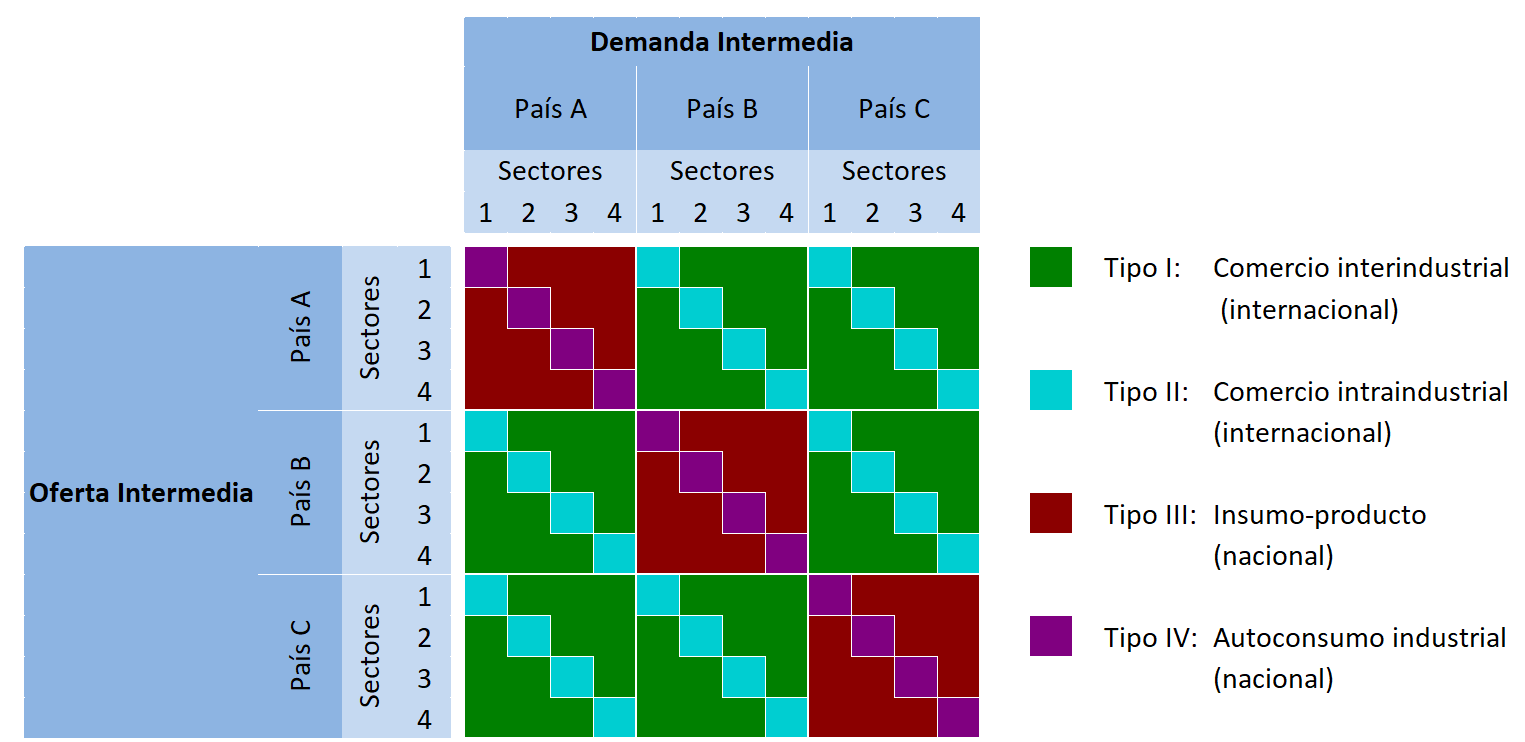
\includegraphics[width=1\linewidth]{Esquema_TiposComercio_2.png}
	\caption{Comercio intermedio global.}
	\label{Fig_Esquema_TiposComercio}
\end{figure}

La figura \ref{Fig_Comercio_InternoExterno} muestra el porcentaje que representa el comercio nacional e internacional, respecto al comercio intermedio global, durante el periodo de estudio. Aunque los flujos comerciales dentro de los países siguen teniendo la mayor proporción; durante el periodo de 1995 y 2008, el comercio internacional aumentó su participación de forma sostenida, pasando del 10.6\% al 15.1\%. Este periodo estuvo marcado por la creación de la Organización Mundial del Comercio (OMC) el 1° de enero de 1995, el ingreso de China a esta organización el 11 de diciembre de 2001 y la entrada en circulación (física) del Euro el 1° de enero de 2002. El aumento relativo del comercio intermedio internacional indica un fortalecimiento de la globalización y del entrelazamiento de la producción en el mundo. La crisis económica de 2008 fue el punto de inflexión de este proceso, que implicó una caída en el peso relativo del comercio internacional frente al nacional. Después de ese año, la proporciones entre el comercio nacional e internacional han pasado por ciclos, con periodos donde el comercio internacional gana terreno frente al nacional (2009-2012, 2016-2018 y 2020-2022); y periodos donde retrocede (2012-2016, 2018-2020).


\begin{figure}[H]
	\begin{subfigure}{\textwidth}
		\centering
		
\includegraphics[width=\textwidth]{Comercio_InternoExterno.png}
		\caption{División nacional / internacional}
		\label{Fig_Comercio_InternoExterno}
	\end{subfigure}
	\begin{subfigure}{\textwidth}
		\centering
		
\includegraphics[width=\textwidth]{TipoComercio.png}
		\caption{Peso relativo por tipo de comercio}
		\label{Fig_TipoComercio}
	\end{subfigure}
	\caption{Evolución del comercio intermedio global}
\end{figure}

Una revisión más detallada de los datos sugiere que la crisis de 2008 no implicó un retroceso permanente en la globalización, pero si una reconfiguración de las cadenas globales de valor. En la figura \ref{Fig_TipoComercio} aparece el peso relativo de cada tipo de comercio intermedio. El primer bloque, correspondiente al porcentaje del comercio insumo-producto nacional, presenta una caída sostenida de 1995 ($71.5\%$) a 2008 ($66\%$); y posteriormente parece estabilizarse alrededor del $67\%$. Por otra parte, los pesos relativos del comercio de tipo I y IV ponen de manifiesto que la pérdida del peso relativo en el comercio interindustrial internacional a partir de 2018 fue ocupada por el crecimiento del autoconsumo industrial (nacional). Esto podría indicar un proceso de especialización y fortalecimiento de las capacidades productivas domésticas, a la par de un reforzamiento de la integración vertical transfronteriza de las cadenas productivas.


\section{Análisis global}

\subsection{Metodología}

Para la detección de bloques comerciales se aplicaron los algoritmos de Louvain y Leiden, descritos en la sección \ref{LeidenLouvain}, a la red de insumo producto internacional durante el periodo 1995-2022. Se definieron tres particiones iniciales como punto de partida de los algoritmos: 
\begin{enumerate}[label=\alph*)]
	\item Por país, esto es, al inicio todos los sectores de un mismo país forman una comunidad; por lo tanto, el algoritmo comienza con 80 clústeres.
	\item Por sector, es decir, todos los vértices que pertenecen al mismo sector, aunque a diferentes países, conforman un clúster, lo que da lugar a 50 clústeres iniciales
	\item Por país-sector, en este caso cada vértice individual constituye su propia comunidad. 
\end{enumerate}
Debido al componente aleatorio de los algoritmos, por cada año, partición inicial y método utilizado, se ejecutaron 30 iteraciones y se reportó la partición con mayor modularidad ponderada y dirigida \eqref{C3_eq_modularity_directed_weighted}. Como método de validación de la modularidad como medida de calidad de las particiones en la red insumo-producto internacional se compararon los resultados obtenidos por los algoritmos con la modularidad correspondiente a las tres particiones iniciales.

El análisis computacional se llevó a cabo en una computadora Dell Precision~3680, equipada con 128~GB de RAM y un procesador Intel Core i9--14900k; mientras que el código fue implementado en Python~3.12.
%El código fue implementado en Python~3.12.
% Además se compararon la modularidad de las particiones resultantes por los algoritmos con la modularidad de cada una de las particiones iniciales. 
 
\subsection{Resultados}


El primer resultado encontrado es que la red insumo-producto internacional tiene una fuerte estructura comunitaria en todo el periodo de estudio, dado que los valores observados de la modularidad se encuentran entre 0.73 y 0.80.\footnote{Los valores exactos de la modularidad máxima y el correspondiente número de comunidades, por año y tipo de partición, se encuentran en la tabla \ref{Resultados_ModularidadClústeres}.} Estos valores son consistentes con los obtenidos por \textcite{Kireyev2022} para los años 2000-2014, y son superiores a los que se han encontrado en otras redes con estructura comunitaria bien definida (entre 0.3 y 0.7), como reporta \textcite[p.~7]{Newman2004}. En la figura \ref{Fig_ModularidadMaxima} se presenta el valor de la modularidad máxima encontrada por el algoritmo de Leiden por cada año. Los colores representan la partición o particiones iniciales que alcanzaron tal valor máximo. En la mayoría de los años (19 de 28), los tres tipos de partición inicial alcanzaron, en alguna de las 30 iteraciones, el valor máximo de modularidad. Esto indica que los resultados son robustos, ya que son independientes de cómo se inicialice el algoritmo; ya sea dividiendo la red por país, por sector o por  vértices individual, la estructura comunitaria detectada es la misma. \textcolor{blue}{También es interesante el hecho de que, salvo para 2019, la partición inicial por sector siempre encontró la mejor partición. Esto es, al iniciar el algoritmo todos los vértices de un mismo sector, pero de diferentes países, forman una comunidad; mientras que el proceso de búsqueda local multinivel es capaz de pasar de esta estructura artificial a la división real por bloques económicos.}
% En los años donde esto no ocurre la diferencia es pequeña.

El segundo hallazgo más importante es que, al igual que en los trabajos de  \textcite{Cerina2015, Kireyev2022}, los bloques comerciales identificados tienen una base netamente nacional o regional. Esto significa que los clústeres corresponden a la unión de los sectores económicos de un país o de un conjunto de países, como puede comprobarse en las figuras del apéndice \ref{Apendice3}. Si bien la mayoría de los sectores de un país pertenecen a una misma comunidad, en algunos casos, existen sectores económicos que están más vinculados a otros bloques comerciales que al mercado nacional. Por ejemplo, aunque en 2022 las economías de Canadá, México y Estados Unidos forman, cada una, su propio bloque comercial, la extracción de petróleo crudo y gas natural de México y Canadá aparece dentro de la comunidad formada por los Estados Unidos. Otro ejemplo de ese mismo es la situación de Camboya: la mayor parte de su economía se encuentra integrada a un bloque comercial junto a las economías de Corea del Sur y Vietnam; mientras que su industria maderera y de productos de caucho y plástico están más vinculados a los Estados Unidos. Por otra parte, los servicios  de mensajería, telecomunicaciones, tecnología e información, así como de actividades profesionales científicas y técnicas forman parte del bloque comercial encabezado por Singapur (véase la figura \ref{Fig_2022_comunidades}).  %\textcolor{blue}{Explicar los bloques formados por la unión de países y los formados por la economía de un solo país.}

\begin{figure}[H]
	\begin{subfigure}{.95\textwidth}
		\centering
		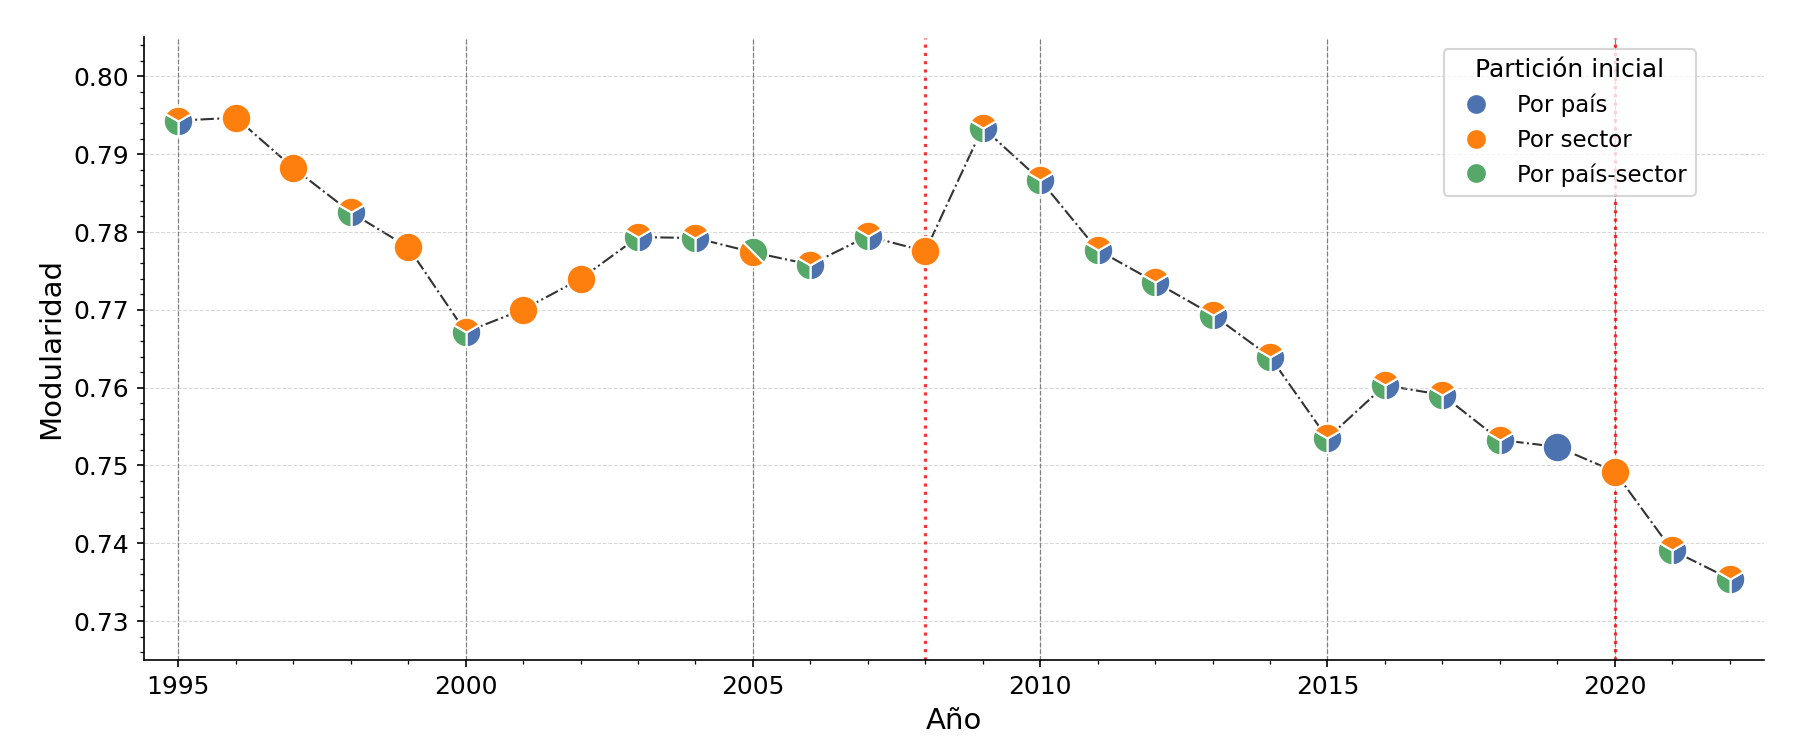
\includegraphics[width=\textwidth]{ModularidadMaxima.png}
		\caption{Modularidad por partición inicial}
		\label{Fig_ModularidadMaxima}
	\end{subfigure}
	\begin{subfigure}{.95\textwidth}
		\centering
		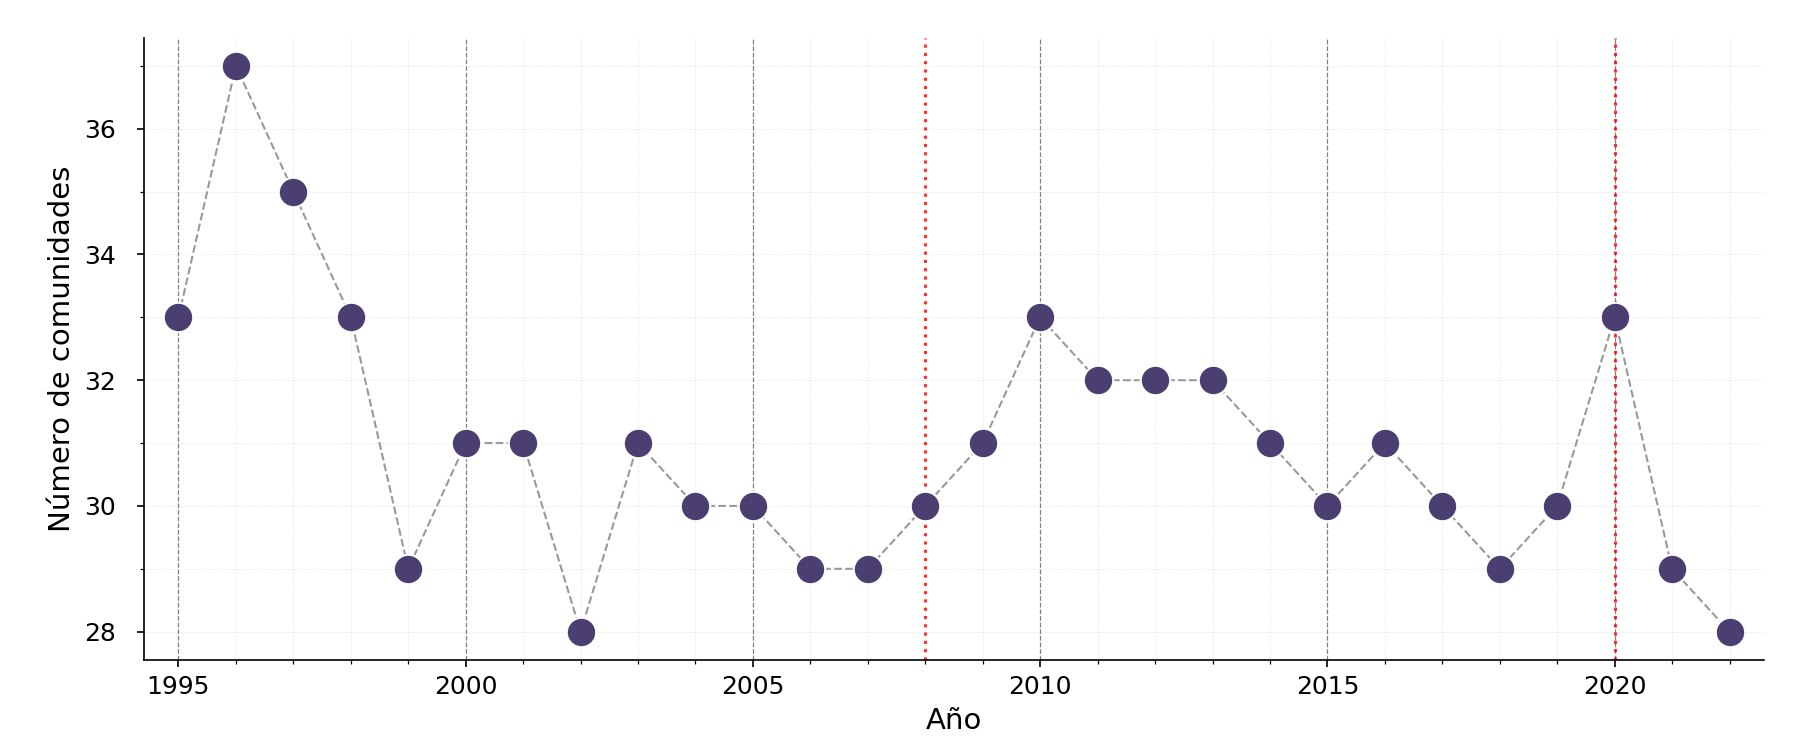
\includegraphics[width=\textwidth]{Clusteres.png}
		\caption{Número de comunidades identificadas}
		\label{Fig_NumeroComunidades}
	\end{subfigure}
	\caption{Resultados del algoritmo de Leiden.}
	\label{Fig_ResultadosLeiden}
\end{figure}

El número de comunidades identificadas presenta alta variabilidad de un año a otro, como puede verse en la figura \ref{Fig_NumeroComunidades}. Sin embargo, pueden observarse algunas tendencias. En primer lugar, una reducción del número de comunidades detectadas, que hasta antes de 1999 eran 33 o más, mientras que posterior a ese año, se encuentran alrededor de 30. \textcolor{blue}{Esta tendencia podría ser la causa de la disminución de la modularidad máxima observada en la figura \ref{Fig_ModularidadMaxima}, ya que la fusión de dos clústeres de una partición, suponiendo una red y pesos dados, conlleva a una disminución de la modularidad. Además, es posible observar que durante los años posteriores a la crisis económica internacional de 2008 y durante la pandemia de 2020, el número de comunidades aumenta. Esto podría ser el resultado de un debilitamiento en los vínculos de algunos bloques regionales derivados de las perturbaciones en el comercio internacional.} % Por ejemplo.


Desde el punto de vista computacional, las particiones obtenidas mediante el algoritmo de Leiden presentan valores de modularidad superiores a las encontradas por el algoritmo de Louvain (véase la tabla \ref{Resultados_ModularidadClústeres}). Esta diferencia puede atribuirse a las mejoras que introduce el algoritmo de Leiden en los procesos de búsqueda local y de refinamiento de las soluciones, como se describe en la sección \ref{LeidenLouvain}. Aunque la diferencia anual en el mejor valor de modularidad entre ambos algoritmos es muy reducida, con un promedio de 0.0002, esta diferencia tiene un impacto significativo en el número de comunidades identificadas, aumentado o disminuyendo hasta en dos comunidades respecto de la mejor partición encontrada.

En cuanto al tiempo de ejecución, el algoritmo de Leiden tiene un comportamiento estable, con un tiempo de ejecución entre 2.3 y 11.1 segundos, y un promedio de 5.2 segundos. Además, estos tiempos son similares, independientemente del tipo de partición inicial, con una ligera reducción cuando se inicia con la partición por país. Por el contrario, los tiempos de ejecución del algoritmo de Louvain muestran alta variabilidad. Cuando se inicializa el algoritmo con la partición por sector, el tiempo de ejecución es muy breve, con un promedio de 0.3 segundos, lo cual podría indicar una rápida convergencia a soluciones de mala calidad. En el caso de la inicialización por país, el tiempo promedio también es reducido (0.4 s.), pero con algunas instancias donde el tiempo llega a extenderse hasta los 15.7 segundos. Por último, la inicialización con cada vértice como su propia comunidad es la que tarda más, con un promedio de 14 segundos y algunas instancias donde supera el minuto. Esto último deriva de la búsqueda exhaustiva de movimientos factibles que realiza el algoritmo de Louvain, sin que mejore la calidad de las soluciones. En la figura \ref{Fig_TiemposAlgoritmos} se presentan los detalles del tiempo de ejecución de cada algoritmo por tipo de partición inicial. En todo caso, es de resaltar que la detección de comunidades pueda realizarse en cuestión de unos pocos segundos, considerando que se trata de redes con más de 7 millones de aristas dirigidas.

\begin{figure}[h]
		\centering
		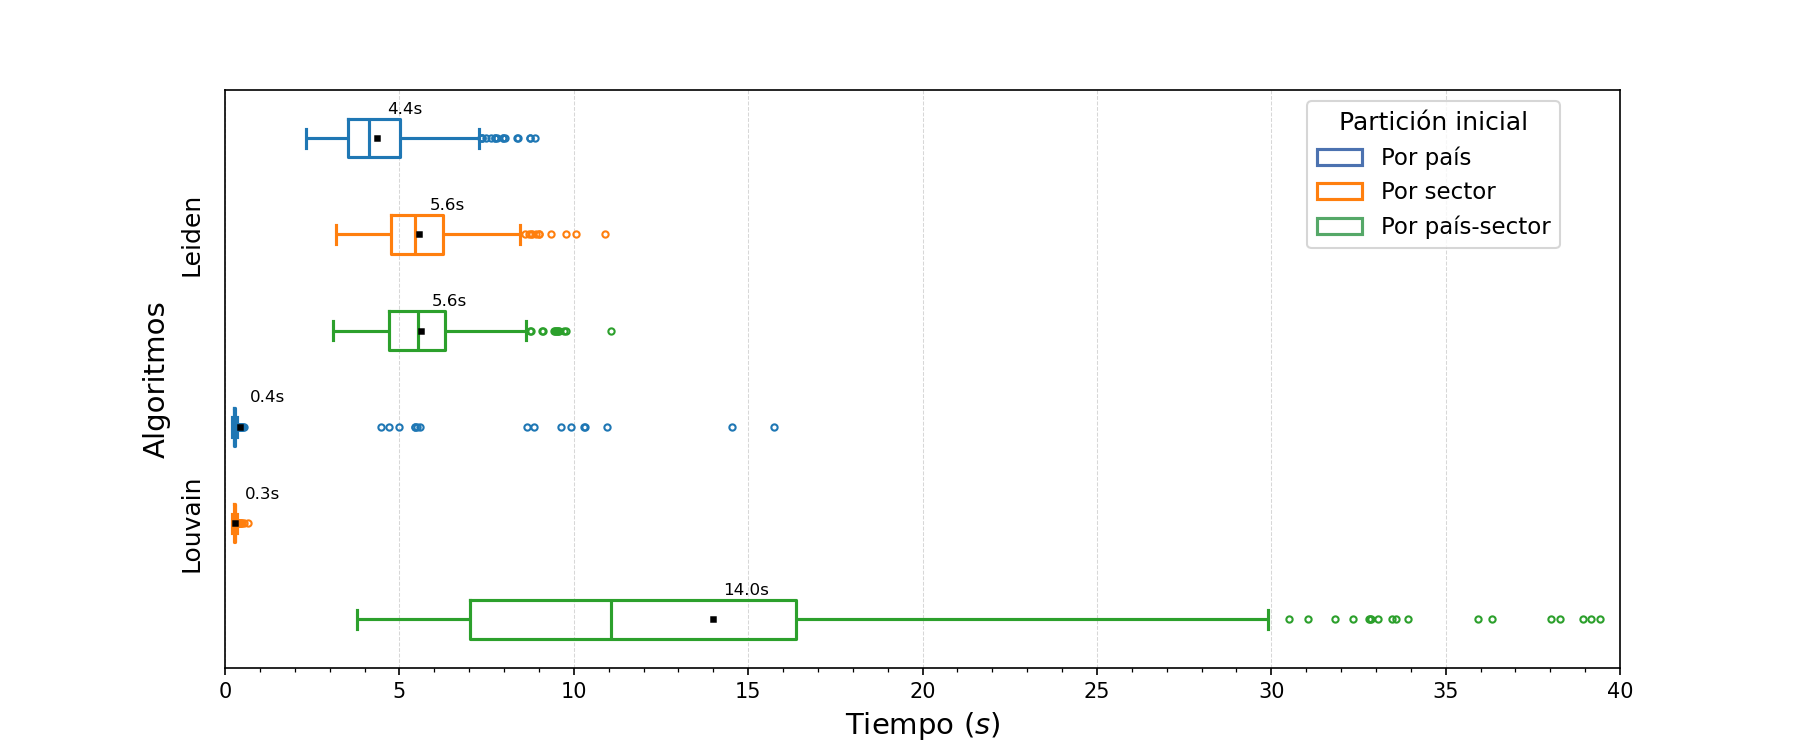
\includegraphics[width=\textwidth]{ComparacionAlgoritmos_Tiempo.png}
		\caption{Tiempo de ejecución de los algoritmos de Leiden y de Louvain}
		\label{Fig_TiemposAlgoritmos}
\end{figure}

Como ejercicio de validación de la modularidad se calculó su valor para las tres particiones iniciales consideradas en el análisis en cada año. La modularidad de la partición donde cada país es su propia comunidad se encuentra siempre por debajo de los valores obtenidos por los algoritmos de Leiden y Louvain, como se observa en la tabla \ref{Resultados_ModularidadClústeres}. En promedio,  la modularidad de las particiones por país es 0.71\% menor a la obtenida por el algoritmo de Leiden. Esto significa que, de forma global, los bloques comerciales detectados tienen mejor interacción, que considerar la economía dividida simplemente por fronteras nacionales. En contraste, la modularidad de la partición por sector y por vértices individuales (país-sector) tienen valores muy bajos cercanos a 0 (en promedio .185 en ambos casos). Esto implica que la densidad de enlaces dentro de estas divisiones es indistinguible de la densidad que tendría una partición aleatoria de los vértices, validando la capacidad de la modularidad para identificar estructuras artificiales. \textcolor{blue}{[Falta calcular la modularidad de una partición por grandes grupos de sectores económicos, equivalentes a las letras del ISIC-4: A (agropecuario), B(extraccion minera), C(industria), D (electicidad, gas), E agua, F Construccion, G (Comercio), H (transporte), I (alojamiento y comida), J (editorial, radifufson telecomunicaciones, tecnología e información), K (financieras), L (inmobiliarias), M (profesionales), N (adm), O, (publica), P (educacion), Q (salud), R (artes), S(otros), T (domesticos.)]}

\graphicspath{
	{../analysis_normalized/images/}
}
\begin{figure}[h]
	\centering
	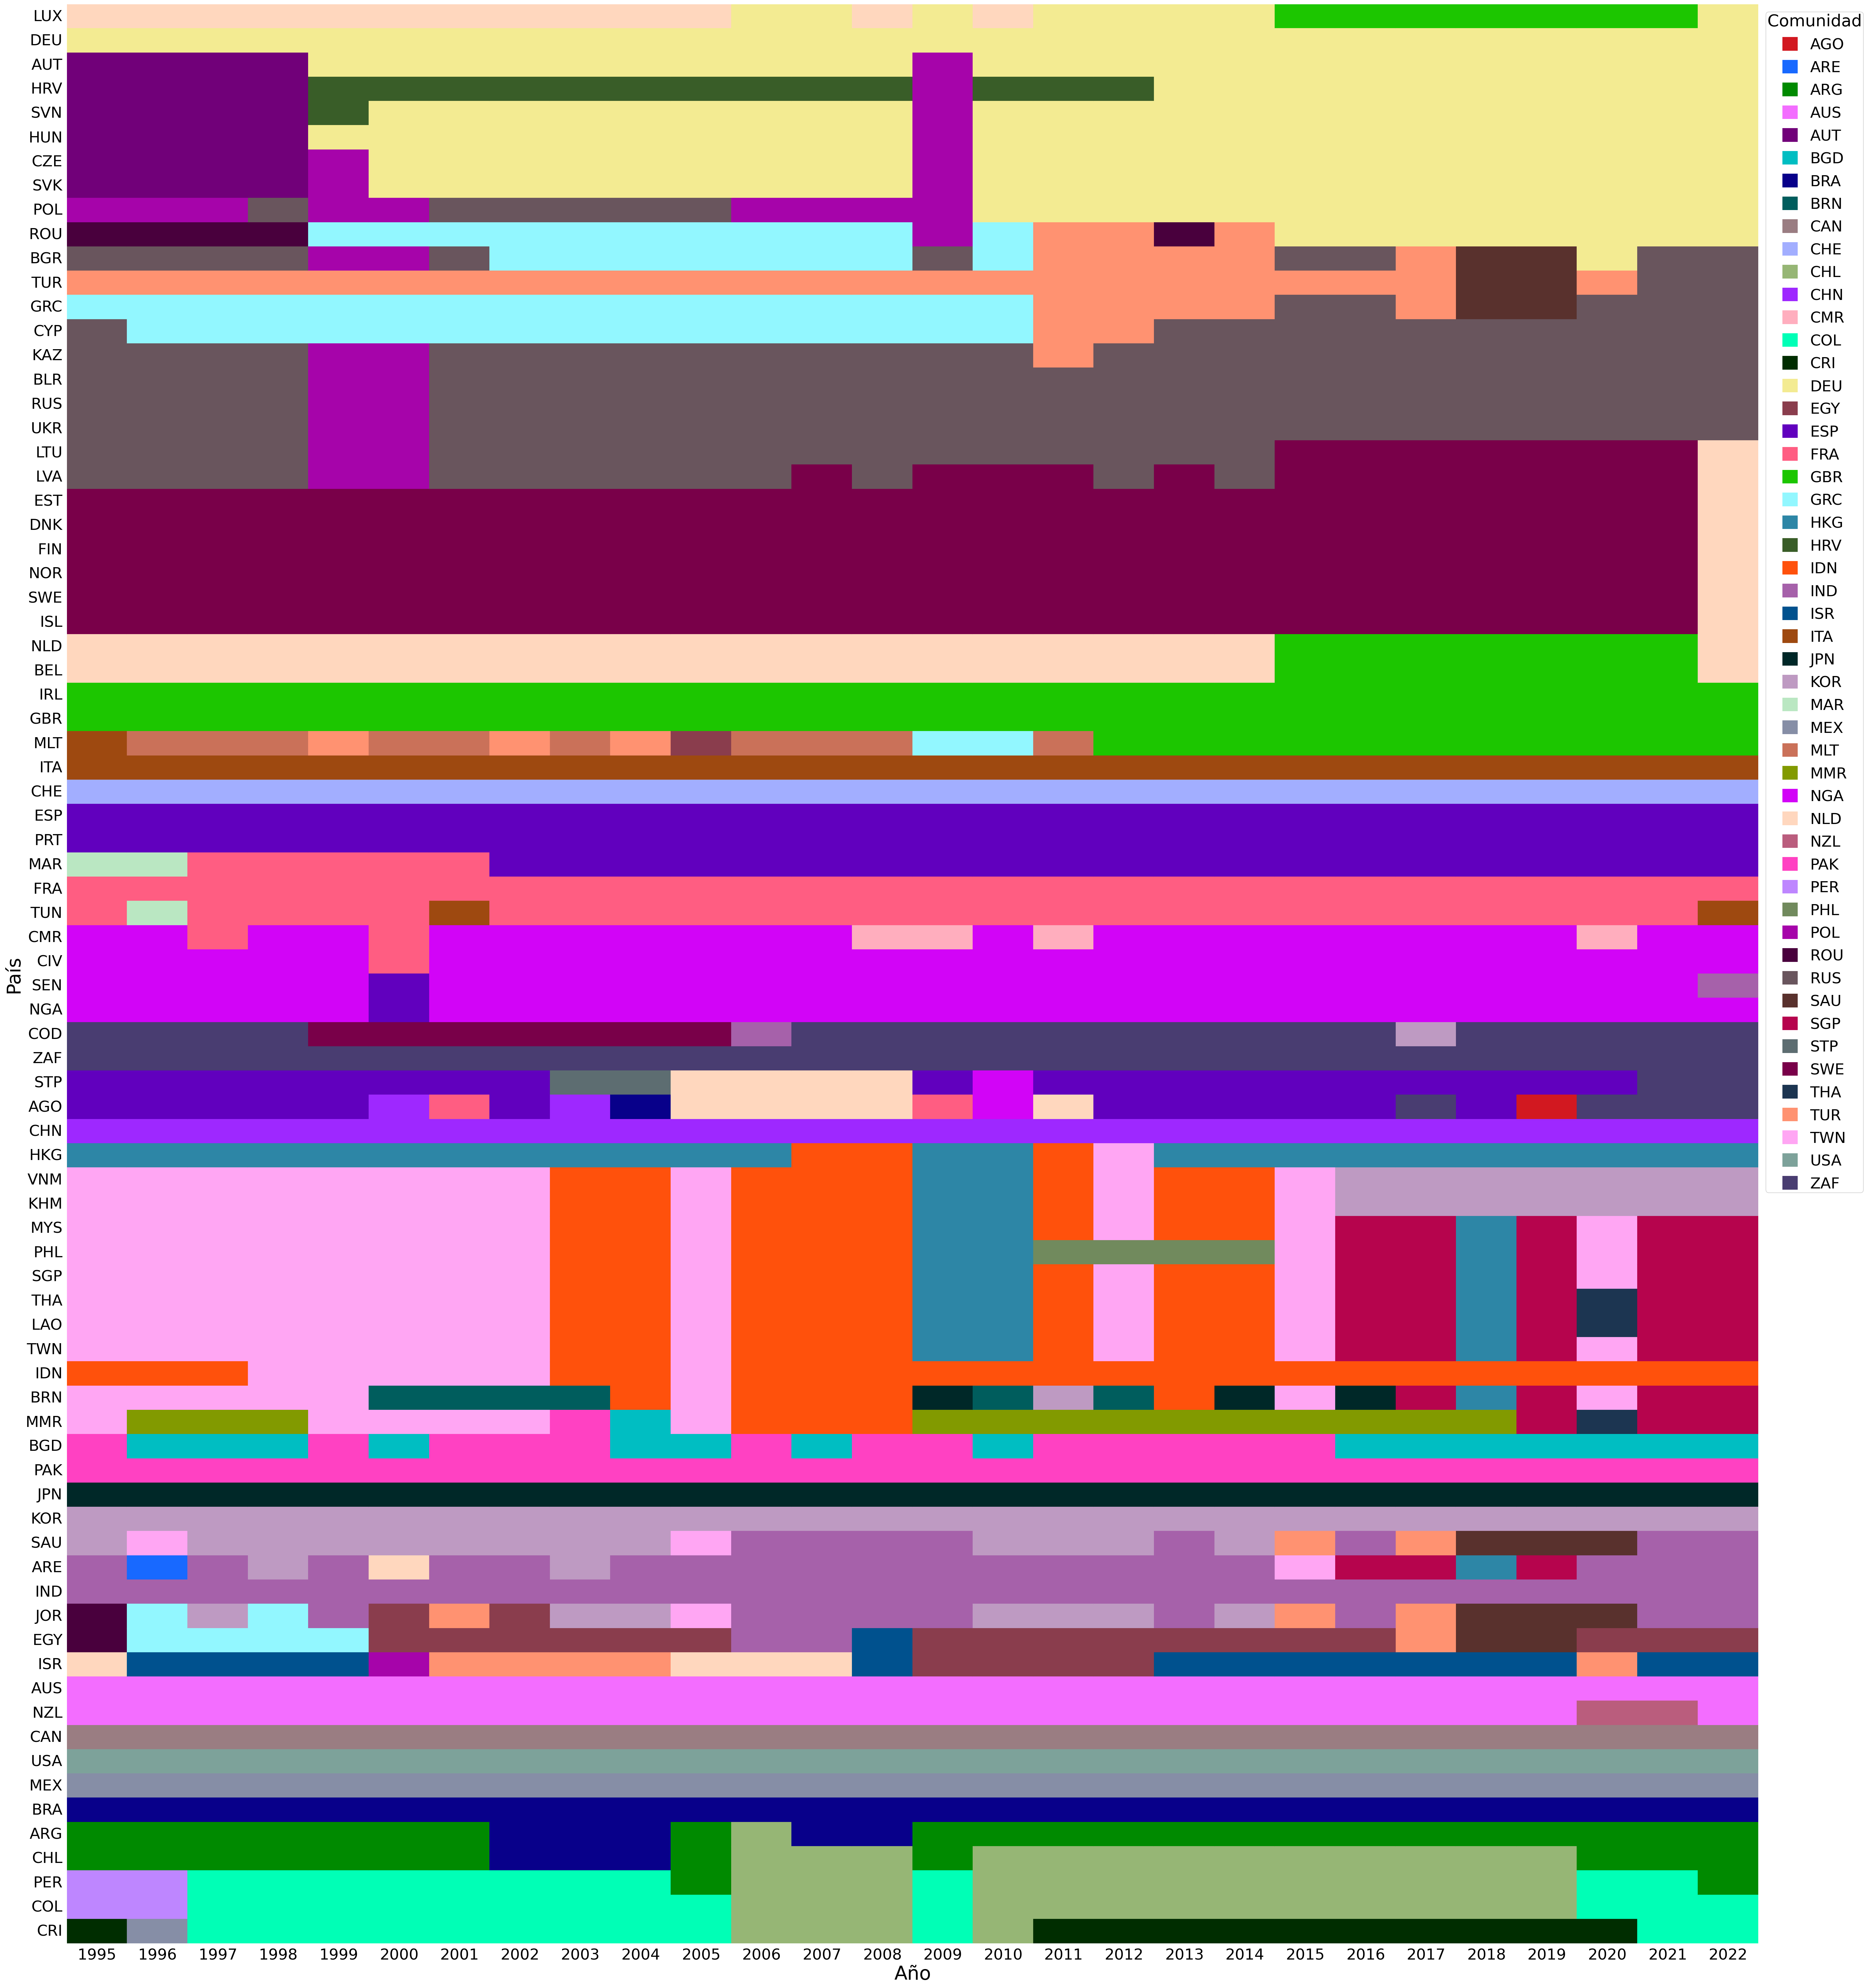
\includegraphics[width=1.1\linewidth]{ComunidadesPorPais.png}
	\caption{\textcolor{blue}{La gráfica muestra a que bloque está integrado la mayoría de la economía de un país. Esto es a que bloque pertenece el 50\%+1 de los sectores de un país. Puede verse cuando dos bloques se unifican. Por ejemplo a partir de 2000, los paies de Europa central y alemania forman un bloque. También se ve cuando un país deja de estar dentro de un bloque por ejemplo, Lituania, letonia y polonia dejan de estar en el bloque de rusia a partir de 2015.}}
\end{figure}

% Calcular modularidad de dividir la economía en bloques de sectores. A ( agropecuario), B(extraccion minera), C(industria), D (electicidad, gas), E 8agua, F Construccion, G (Comercio), H (transporte), I (alojamiento y comida), J (editorial, radifufson telecomunicaciones, tecnología e información), K (financieras), L (inmobiliarias), M (profesionales), N (adm), O, (publica), P (educacion), Q (salud), R (artes), S(otros), T (domesticos.)


\section{Análisis regional}

 %\textcolor{blue}{Analizar la evolución histórica de algunos bloques. En particular, de la Unión Europea, el TLCAN y ASEAN}.








	\clearpage
\subsection{Sudeste asiático: ASEAN}

La \acrfull{asean} se estableció en 1967, enmarcada por la guerra de Vietnam, por 5 países: Malasia, Indonesia, Filipinas, Singapur y Tailandia. Su objetivo principal era promover la paz y la estabilidad en la región, así como fomentar la cooperación económica, social, cultural, técnica y educativa entre los países miembro. Posteriormente, se unieron a la asociación otros 6 países: Brunei Darussalam en 1984, Vietnam en 1995, Laos y Myanmar en 1997, Camboya en 1999 y, recientemente, en 2025, Timor Oriental \parencite{ASEAN}. Durante los primeros años de existencia, la cooperación económica en la \gls{asean} fue promovida a través de un \gls{pta} que tenía como uno de sus principales objetivos reducir los aranceles sobre ciertos productos industriales. Sin embargo, este objetivo no logró materializarse debido, principalmente, a que los países integrantes de la \gls{asean} siguieron una estrategia de industrialización por sustitución de importaciones durante esos años. La integración económica de la \gls{asean} comenzó formalmente con la creación del \gls{afta} en 1992. Desde entonces, el proceso de integración regional ha pasado por tres fases principales: una etapa inicial caracterizada por la consolidación del \gls{afta} de 1992 a 2002; después, una fase marcada por la conformación de la \gls{aec} entre 2003 y 2015; y una tercera etapa centrada en la implementación del Plan Maestro de la \gls{aec} 2025 a partir de 2016 \parencite[pp.~25--26]{Ishikawa2021}.

El \gls{afta} fue creado como respuesta al surgimiento de otros bloques regionales, como el \gls{tlcan} y la expansión de la \gls{ue}. Sus objetivos principales fueron la creación de un mercado único, la atracción de inversiones extranjeras directas en la región y la expansión del comercio y las inversiones intrarregionales. El principal mecanismo para lograr estos objetivos fue el \gls{cept}, el cual permitió una reducción gradual de los aranceles dentro de la \gls{asean} hasta alcanzar una tasa arancelaria entre el 0 y el 5\%. Para acceder a estas preferencias, los bienes debían cumplir reglas de origen, basadas en un contenido regional acumulado de al menos 40\% \parencite{ASEAN_CEPT}. Sin embargo, a diferencia de la \gls{ue}, el \gls{afta} no implicó un arancel externo común a las mercancías importadas de fuera de la asociación \parencite{ASEAN_AFTA}. El \gls{afta} logró que los aranceles en la \gls{asean}6 (Brunei, Indonesia, Malasia, Filipinas, Singapur y Tailandia) se redujeran a menos del 5\% en 2003, cinco años antes de lo planificado, y se eliminaran en prácticamente todas las líneas arancelarias en 2010. \textcite{Ishikawa2021} sostiene que el éxito del \gls{afta} se debió en gran medida a que se trató de un proceso gradual y flexible de liberalización, que consideró los diferentes niveles de desarrollo económico e industrial entre los países miembro. Este proceso de liberalización gradual y flexible fue favorecido por el diseño institucional del \gls{afta}, que contempló calendarios diferenciados, listas de exclusión y un trato especial para los países con menores niveles de desarrollo. El esquema \gls{cept}-\gls{afta} fue notificado ante el \gls{gatt} bajo la Cláusula de Habilitación, la cual permite acuerdos comerciales preferenciales entre países en desarrollo con requisitos menos estrictos que los establecidos en el artículo XXIV para las zonas de libre comercio y las uniones aduaneras.

La integración económica de la \gls{asean} se amplió durante la década de 1990, más allá de la liberalización comercial. En 1995 se estableció el \gls{afas}, orientado a reducir las restricciones al comercio regional de servicios \parencite{ASEAN_services}. Al año siguiente, se creó el esquema \gls{aico}, que promovió las actividades industriales conjuntas y la formación de redes regionales de producción; y en 1998 se constituyó el Área de Inversión de la \gls{asean}, y después fue sustituida por el \gls{acia} en 2009, con el propósito de liberalizar, facilitar y proteger las inversiones intrarregionales \parencite[p.~16]{ASEAN_AIR2012}. En conjunto, estos instrumentos fortalecieron el comercio, la inversión extranjera y la consolidación de cadenas regionales de valor.

La \acrfull{aec} fue planteada por primera vez en 2003 durante la IX Cumbre de la asociación, con el objetivo de transformar a la \gls{asean} en una región con libre circulación de bienes, servicios, inversiones, mano de obra calificada y una mayor libertad para los flujos de capital. Como parte de esta estrategia, se firmó el Acuerdo Marco de la \gls{asean} para la Integración de Sectores Prioritarios, que incluyó los productos agroindustriales, las industrias automotriz, electrónica y textil, la pesca, los productos derivados del caucho y la madera, el transporte aéreo, las tecnologías de la información y la comunicación, los servicios de salud, el turismo y la logística. En la XII Cumbre de la \gls{asean} celebrada en 2007, se aceleró el compromiso de establecer la \gls{aec} para 2015. Estos acuerdos también contemplaban el mejoramiento de la infraestructura de transporte y comunicaciones intrarregional, así como el establecimiento de mecanismos de interconexión energética \parencite{Ishikawa2021, ASEAN_Vision_2020}.

La \gls{aec} fue formalmente establecida en 2015, conforme al calendario previsto, aunque no todas las medidas acordadas en el Plan Maestro de la \gls{aec} 2015 fueron implementadas. Un elemento clave que ayudó al cumplimiento de este compromiso fue la sustitución del esquema \gls{cept} por el \gls{atiga} en 2010. El logro más importante del \gls{aec} fue la eliminación de aranceles, alcanzando una tasa de liberalización comercial\footnote{Porcentaje de líneas arancelarias sujetas a eliminación} del 98.6\% \parencite[p.~29]{Ishikawa2021}. El ATIGA también abarcó la facilitación de trámites aduaneros y el reconocimiento mutuo de normas \parencite[p.~16]{ASEAN_AIR2012}. En contraste, existen otros elementos que han avanzado con mayor lentitud, como la reducción de barreras no arancelarias y la liberalización del comercio de servicios y de las inversiones \parencite[p.~29]{Ishikawa2021}.

Aunque los marcos de integración económica de la \gls{asean} no incluyen un arancel común al exterior, la Asociación ha establecido de manera conjunta acuerdos de libre comercio y de asociación económica con otros países asiáticos bajo el esquema ASEAN$+1$. En particular, se establecieron acuerdos de libre comercio con la República Popular China, Corea del Sur, Japón, Australia y Nueva Zelanda, India y Hong Kong \parencite{ASEAN_FTA}. A su vez, en 2019 concluyeron las negociaciones sobre la conformación de la \gls{rcep}, un acuerdo de libre comercio multilateral entre los Estados miembros de la \gls{asean} y China, Japón, Corea del Sur, Australia y Nueva Zelanda. El objetivo del \gls{rcep} es armonizar los acuerdos de libre comercio existentes de la ASEAN$+1$ en un acuerdo unificado, con un conjunto único y coherente de normas comerciales para la región \parencite[pp.~92--94]{ASEAN_Digital2025}.
% ASEAN-CHINA FTA (ACFTA)effect 2004
% ASEAN-Korea FTA (AKFTA) effect 2007
% ASEAN-Japon FTA (AJFTA) effect 2008
% ASEAN-Australia-New Zealand FTA (AANZAFTA) effect 2010
% ASEAN-INDIA (AIFTA) effect 2010
% ASEAN-Hong-Ling (AHFKTA), 2019

%Después del establecimiento de la \gls{aec}, la integración económica regional se profundizó mediante nuevos mecanismos de facilitación comercial, apertura de servicios y vinculación externa. La \gls{asean} Single Window fue desarrollada para permitir el intercambio electrónico de documentos comerciales y aduaneros, agilizando el despacho de mercancías entre los países miembros; el \gls{atisa} amplió los compromisos regionales para reducir las barreras regulatorias al comercio de servicios; y el \gls{rcep} extendió la integración hacia los principales socios económicos de la región mediante disposiciones sobre bienes, servicios, telecomunicaciones y comercio electrónico. En conjunto, estos instrumentos contribuyeron a reducir los costos de las operaciones transfronterizas y a fortalecer la participación de la \gls{asean} en las cadenas regionales de valor \parencite[pp.~94--95]{ASEAN_Digital2025}

% 
% En 2018, la tasa de liberalización alcanzó el 99.3\% para el ASEAN6 y el 98.6\% para el ASEAN en su conjunto. \cite{Ishikawa2021} 
% Al año siguiente, durante la X Cumbre se firmó el Acuerdo marco de la ASEAN para la Integración de Sectores Prioritarios, que comprendía el periodo de 2004 a 2010, designando como sectores prioritarios los productos agropecuarios, pesca, industriales (automotriz, productos de caucho, textiles y prendas de vestir, de madera), transporte aéreo, telecomunicaciones, sanidad y turismo; previendo su plena integración para 2010 \parencite[p.~28]{Ishikawa2021}.

% La CEA aspira a consolidar a la ASEAN como un mercado único y una base de producción, una región económica altamente competitiva, una región de desarrollo económico equitativo y una región plenamente integrada en la economía global (nota 17). Estos cuatro objetivos constituyen los cuatro pilares del Plan de la CEA.

Por su parte, el análisis de las comunidades en la red insumo--producto mundial ofrece una oportunidad para evaluar el nivel de integración económica de la \gls{asean} a partir de sus vínculos intersectoriales. En primer lugar, los resultados indican un fuerte nivel de estabilidad en la integración económica de la región, en el sentido de que las economías de la mayoría de países miembros pertenecen al mismo bloque económico durante el periodo estudiado (véase la figura \ref{ComunidadesPorPais_ASEAN}). En segundo lugar, el análisis de comunidades permitió identificar a los países con menor cohesión en la economía regional de la \gls{asean}, a partir del número de años en los que sus economías conforman una comunidad individual: Indonesia (14 años), Myanmar (13 años), Brunei (6 años) y Filipinas (4 años). En contraste, también se observaron vínculos de integración con economías externas al \gls{asean}, particularmente Taiwán y Hong Kong. El caso de Taiwán resulta relevante, ya que durante todo el periodo estudiado formó parte del bloque económico asociado a la mayoría de los países de la \gls{asean}. Finalmente, los resultados no reflejan una asociación directa con el establecimiento de acuerdos de libre comercio formales. Por ejemplo, aunque la \gls{asean} ha formalizado áreas de libre comercio con países como China o India, esto no se ve reflejado directamente en la integración de sus economías en la misma comunidad. En el caso de Hong Kong, su integración al bloque económico asociado a la \gls{asean} ocurre años antes de la firma del acuerdo en 2019. Solo en el caso de Corea del Sur, las economías de Vietnam y Camboya presentan una integración estable a su comunidad a partir de 2016. Por el contrario, aunque la \gls{asean} no cuenta con un tratado de libre comercio con Taiwán, su economía se encuentra estrechamente vinculada a la de los países de la \gls{asean} a través de sus flujos intersectoriales.

\begin{figure}[H]
	\centering
	
\includegraphics[width=\textwidth]{images/ComunidadesPorPais_ASEAN.png}
	\caption{Integración de las economías de la ASEAN en bloques productivos.$^{*}$}
	\label{ComunidadesPorPais_ASEAN}
	
	\caption*{\footnotesize $^{*}$ El color en la gráfica depende del país al que pertenece el vértice con mayor fuerza de salida intrarregional en ese año. Eso puede causar un efecto visual de contraste en una misma comunidad. Como muestra de ello, en 2005 y 2006 todos los países de la \gls{asean} más Taiwán formaron una sola comunidad, solo que en 2005 el nodo con mayor fuerza de salida era de Taiwán y en 2006 de Indonesia, lo cual explica el cambio abrupto de color. Por lo tanto, la gráfica no debe evaluarse únicamente por el color, sino por los países que pertenecen a un mismo color.}
\end{figure}
%\begin{figure}[H]
%	\centering
%	
\includegraphics[width=\textwidth]{images/ComunidadesPorPais_ASEAN.png}
%	\caption{Integración de las economías de la ASEAN en bloques comerciales$^{*}$.}
%	\label{ComunidadesPorPais_ASEAN}

%	\caption*{\footnotesize $^{*}$ Las filas representan países y las columnas años. El color de cada celda corresponde al color de la comunidad a la cual pertenece la mayoría de los sectores económicos de un país en el año correspondiente. Cada comunidad se identifica con el país del vértice con la mayor fuerza de salida.}
%\end{figure}


La dinámica de las comunidades identificadas permite establecer cuatro periodos en el proceso de integración económica del sudeste asiático:
\begin{itemize}
	\item Formación del núcleo productivo regional (1995--2004).
	%un proceso de fortalecimiento del núcleo productivo regional, con incorporaciones y separaciones temporales. 
	Durante este periodo, el bloque económico asociado al \gls{asean} se compone de las economías de Vietnam, Camboya, Malasia, Filipinas, Singapur, Tailandia, Laos y Taiwán. Por su parte, Indonesia, Brunei y Myanmar forman comunidades individuales en algunos lapsos de años. Este periodo coincide con la consolidación del \gls{afta} y la reducción gradual de aranceles en la región. Además, en estos años hay muchos sectores individuales de los países de la \gls{asean} que forman parte de otras comunidades externas a la región, principalmente en las comunidades de Hong Kong y Japón (véase la figura \ref{DiagramaSankey_ASEAN} y el apéndice \ref{Apendice3}).\footnote{Dentro de este conjunto, destacan la extracción de minerales metálicos (B07) de Filipinas que perteneció a la comunidad de Japón de 1995 a 1998; la extracción de petróleo crudo y gas natural (B06) de Brunei que estuvo integrada a la comunidad de Japón en los años 2001 y 2003; y las actividades postales y de mensajería (H53) de varios países de la \gls{asean} que durante todo el periodo estuvieron en la comunidad encabezada por Hong Kong.}
	
	\item Máxima cohesión regional (2005--2008). En estos años, los 10 países de la \gls{asean} forman parte de la misma comunidad, junto con Taiwán; y en 2007 y 2008, también junto a Hong Kong. Este periodo se encuentra enmarcado por los trabajos de la \gls{asean} de establecer su \acrfull{aec}. 
	
	\item Reconfiguración e inestabilidad (2009--2015). El bloque económico asociado al \gls{asean} se reduce, con la salida de Myanmar, Indonesia y Filipinas de la comunidad. Esto podría reflejar las consecuencias que tuvo la crisis internacional de 2008 en el proceso de integración regional.
	 
	\item Fragmentación y formación de bloques subregionales (2016--2022). Se observa la integración estable de las economías de Vietnam y Camboya a la comunidad de Corea del Sur. Durante este periodo, nuevamente hay sectores individuales de los países de la \gls{asean} que se integran a otras comunidades, como las de China, Estados Unidos, Reino Unido y Japón (véase la figura \ref{DiagramaSankey_ASEAN} y el apéndice \ref{Apendice3}).\footnote{Por ejemplo, la extracción de minerales metálicos (B07) de Filipinas estuvo alineada con la economía de China a partir de 2017; y la industria de productos de madera (C16) y de caucho y plástico (C22) de Camboya se integró al bloque productivo estadounidense desde 2020.}
\end{itemize}

\begin{figure}[H]
	\centering
	
\includegraphics[width=1\textwidth]{sankey_diagrams/asean_all.png}
	\caption{Evolución de la pertenencia a comunidades de los sectores económicos de los países de la \gls{asean}.}
	\label{DiagramaSankey_ASEAN}
\end{figure}

La figura \ref{Mapa_Comunidades_ASEAN} muestra el mapa de las comunidades en el sudoeste asiático en tres momentos: 1995, 2008 y 2022. Destaca la intensidad de los flujos comerciales entre Taiwán, Tailandia, Malasia y Singapur, los cuales abarcan a la mayoría de los sectores económicos de estos países. Además, dichos flujos presentan una distribución relativamente equilibrada entre los distintos socios comerciales. Esto refleja la profunda interdependencia económica que se ha formado entre estas economías.

\begin{figure}[H] 
	\centering
	\begin{subfigure}{.9\textwidth}
		\centering
		
\includegraphics[width=\textwidth]{images/maps/ASEAN_1995_1.png}
		\caption{1995}
	\end{subfigure}
	\begin{subfigure}{.9\textwidth}
		\centering
		
\includegraphics[width=\textwidth]{images/maps/ASEAN_2008_1.png}
		\caption{2008}
	\end{subfigure}
	\begin{subfigure}{.9\textwidth}
		\centering
		
\includegraphics[width=\textwidth]{images/maps/ASEAN_2022_1.png}
		\caption{2022}
	\end{subfigure}
	\caption{Mapa de las comunidades identificadas en el sudeste asiático.$^{*}$}
	\label{Mapa_Comunidades_ASEAN}
	
	\caption*{\footnotesize $^{*}$ Los sectores económicos se disponen circularmente alrededor del centro del país al que pertenecen y se ordenan en el sentido de las manecillas del reloj. El color de cada sector indica la comunidad a la que pertenece. Las aristas representan únicamente los flujos comerciales cuya magnitud supera el percentil 50 de la distribución regional, y su grosor es proporcional a la intensidad de cada flujo.}
\end{figure}

%Extraccion de mienrales metalicos Filipinas - Japon 1995, 1996, 97, 98


%	 En segundo lugar, el análisis de comunidades muestra que existe una coincidencia entre las fases de integración de la ASEAN que propone \textcite{Ishikawa2021} y la evolución de las comunidades en la región. De 1995 a 2003 se observa que los países de la ASEAN formaron parte de una comu



%\textcolor{blue}{Observaciones: 1) Hay cierta estabilidad en el sentido que la mayoría de los paises de la asean siempre pertenecen a la misma comunidad, aunque la comunidad esté encabezada por otros países. 2) De 1995 a 2002 esta comunidad estuvo encabezada por Taiwán, posteriormentemaoritariamente por indonesia, y luego por Singapur. 3). Indonesi, Bruneii y miarmar son paises que por temporatadas se salen para formar su propia comunidad. Filipinas de 2011 a 2014.}


%Área de Libre Comercio de la ASEAN (AFTA, por sus siglas en ingles):
%Revisar \url{https://fta.miti.gov.my/index.php/pages/view/asean-afta}


%\begin{figure}[H]
%	\centering
%	\begin{subfigure}{.6\textwidth}
	%		\centering
	%		
\includegraphics[width=\textwidth]{images/communities_membership/IDN.png}
	%		\caption{Comunidad encabezada por Indonesia}
	%	\end{subfigure}
%	\par\medskip
%	\begin{subfigure}{.6\textwidth}
	%		\centering
	%		
\includegraphics[width=\textwidth]{images/communities_membership/TWN.png}
	%		\caption{Comunidad encabezada por Taiwán}
	%	\end{subfigure}
%	\par\medskip
%	\begin{subfigure}{.6\textwidth}
	%		\centering
	%		
\includegraphics[width=\textwidth]{images/communities_membership/HKG.png}
	%		\caption{Comunidad encabezada por Hong Kong}
	%	\end{subfigure}
%	\caption{Cantidad de vértices por comunidades del sudeste asiático}
%\end{figure}


	\clearpage
\subsection{América del Norte: TLCAN-TMEC}


En 1986, México se adhirió al \acrfull{gatt}, hecho que marcó un punto decisivo en su proceso de apertura comercial. Después, en 1989 Canadá y Estados Unidos pusieron en vigor un tratado de libre comercio (\acrshort{cusfta}) orientado a eliminar aranceles y reducir barreras comerciales de bienes y servicios. Tanto la apertura comercial de México como la experiencia previa del \acrshort{cusfta} sentaron las bases para la negociación del \acrfull{tlcan} entre México, Estados Unidos y Canadá, que entró en vigor el 1° de enero de 1994 \parencite[p.~170]{Nagy2025}. La negociación del tratado estuvo acompañada de la firma de dos acuerdos de cooperación en materia de regulación laboral\footnote{\gls{alcan}} y ambiental,\footnote{\gls{acna}} debido a la controversia política que rodeó la ratificación del \gls{tlcan} en los Estados Unidos. Sin embargo, ambos acuerdos de cooperación no contaron con fuerza vinculante ni mecanismos de cumplimiento obligatorio \parencite[p.~277, 283]{Stanford2019}. 

El acuerdo entre Canadá y Estados Unidos y la posterior integración de México representaron uno de los primeros ejemplos de acuerdos comerciales regionales que iban más allá de la simple eliminación de aranceles, al incluir una amplia gama de disposiciones regulatorias, mecanismos de protección de la propiedad intelectual y de las inversiones, así como limitaciones a las intervenciones gubernamentales \parencite[pp.~279--281]{Stanford2019}. El documento estaba integrado por 22 capítulos en los que se abordaban diferentes puntos, como el programa de reducción arancelaria, la reducción de barreras no arancelarias, la desregulación industrial, disposiciones para la protección de la inversión extranjera intrarregional, mecanismos para la solución de controversias entre empresas y gobiernos, revisión por paneles binacionales de resoluciones antidumping, entre otros \parencite[véase][]{Stanford2019}. Dos de los mecanismos más importantes del \gls{tlcan} son las normas de \textit{trato nacional} y el \textit{trato de nación más favorecida}, que se encuentran en el capítulo 1 del acuerdo. El primer principio implica que los bienes, servicios e inversiones de empresas de un país del \gls{tlcan} no deben sufrir discriminación debido a su origen nacional. El principio del trato de nación más favorecida establece que cada país dentro del acuerdo debe extender a los otros dos integrantes el trato más favorable que ofrece a países externos al \gls{tlcan} en términos de aranceles y regulación \parencite[p.~21]{Anderson2008}.

La reducción de aranceles se desarrolló de manera gradual. Los aranceles sobre el comercio bilateral entre Canadá y Estados Unidos siguieron el esquema decenal acordado en 1989 en el \acrshort{cusfta}. Por su parte, los aranceles entre México y Estados Unidos y entre México y Canadá siguieron un programa de reducción de diez años a partir de 1993; de tal manera que, para 2003, gran parte de los aranceles sobre el comercio intrarregional se habían eliminado, de acuerdo con \textcite{Stanford2019}. Sin embargo, algunos sectores considerados estratégicos no fueron afectados por el acuerdo, como la industria petrolera mexicana, los servicios culturales canadienses y el transporte aéreo y las radiotelecomunicaciones estadounidenses \parencite[p.~170, 174]{Nagy2025}. Además de la reducción arancelaria, el tratado de libre comercio incluía unas \textit{reglas de origen} que evitaban que los exportadores de fuera de la región aprovecharan el país del \gls{tlcan} con los aranceles más bajos para acceder al mercado regional. Como regla general, al menos el 50\% del costo neto de un producto debe haberse generado dentro de la región, aunque el porcentaje es mucho más alto en la industria automotriz, de autopartes y de calzado \parencite[pp.~170,~182]{Nagy2025}.

%En el caso de algunos productos agrícolas, textiles y automotrices los aranceles se eliminaron gradualmente entre 1994 y 2008 \parencite[p.~170]{Nagy2025}. % Ver seccion 7.2 sobre industrias específicas de Nagy 2025 (174())

En materia energética, el \gls{cusfta} incluía una disposición que garantizaba el acceso estadounidense a los suministros energéticos de Canadá, la cual se mantuvo en el capítulo 6 del \gls{tlcan}. Por el contrario, el tratado protegió explícitamente el derecho de México sobre sus recursos energéticos y la propiedad estatal de \acrshort{pemex} \parencite[p.~282]{Stanford2019}. 

En 2018, se anunció un nuevo acuerdo comercial entre Estados Unidos y México, y un mes después se modificó para integrar también a Canadá. El nuevo acuerdo comercial, denominado \gls{tmec}, se firmó a finales de noviembre de 2018 y se implementó a partir de julio de 2020 \parencite[p.~172]{Nagy2025}. En contraste con el \gls{tlcan}, el \gls{tmec} refuerza la regulación laboral, incluyendo referencias a los derechos de los trabajadores a la asociación, la huelga y la representación sindical democrática \parencite[p.~283]{Stanford2019}. Sin embargo, el nuevo tratado no produjo grandes cambios que profundizaran la integración económica regional, sino que impuso nuevas restricciones y refuerzó algunas características proteccionistas del antiguo acuerdo. Por ejemplo, se elevó la regla de origen en la industria automotriz de un 62.5\% a un 75\%. Además, a diferencia del \gls{tlcan}, el \gls{tmec} tiene una cláusula que estipula la expiración del acuerdo en 16 años y una revisión cada 6 años \parencite[p.~184]{Nagy2025}.% https://www.scielo.org.mx/scielo.php?pid=S1870-35502021000200289&script=sci_abstract&tlng=en

El \gls{tlcan}-\gls{tmec} han incrementado la integración comercial de América del Norte, aunque este proceso se ha desarrollado de forma desequilibrada, centrado en el comercio de México y Canadá con Estados Unidos. Muestra de ello es que las exportaciones de ambos países se dirigen casi por completo al mercado estadounidense: 92.4\% en el caso de México y 97.4\% en el de Canadá. En contraste, las exportaciones estadounidenses destinadas a sus socios regionales se distribuyen en un 39.5\% hacia México y un 60.5\% hacia Canadá \parencite[p.44]{Murillo2022}. Estos datos ilustran cómo la integración regional no se articuló de forma equilibrada entre los tres miembros, sino que se estructuró en torno a dos vínculos bilaterales con Estados Unidos, mientras que el comercio bilateral entre México y Canadá es muy bajo. 
La centralidad estadounidense también se refleja en la composición del valor agregado regional. Una muestra de ello es que en 2015 el 12\% del valor agregado contenido en las exportaciones mexicanas procedía de Estados Unidos; en contraste, la participación mexicana en las exportaciones estadounidenses fue de apenas 1\%. De manera similar, el valor agregado estadounidense representaba el 10\% de las exportaciones canadienses, frente a una participación canadiense de solo un 2\% en las exportaciones de Estados Unidos. En consecuencia, aunque el \gls{tlcan} y el \gls{tmec} han favorecido la formación de una cadena regional de valor, la participación de los tres países en ella es desigual. De acuerdo con \textcite{Murillo2022}, Estados Unidos ocupa una posición central, abasteciendo a sus dos socios regionales de bienes intermedios que, después de ser procesados o ensamblados, son reexportados al mercado estadounidense para su consumo final. México y Canadá, en cambio, presentan una forma de participación más simple, principalmente como exportadores de bienes finales dirigidos a Estados Unidos. En particular, México presenta una integración relativamente superficial en la cadena de valor regional, caracterizada por un bajo contenido de valor agregado interno y una elevada dependencia de los insumos estadounidenses.

El \gls{tlcan} y, posteriormente, el \gls{tmec} pueden ser clasificados como un \gls{fta}, de acuerdo con la clasificación de \textcite{Balassa1961}, debido a que se eliminan las barreras (arancelarias y no arancelarias) al comercio entre los países firmantes, pero cada país integrante mantiene independencia en sus políticas comerciales con países externos. En el caso del \gls{tmec}, algunas industrias están sujetas a excepciones, reservas o disposiciones especiales que limitan la aplicación de las obligaciones generales del tratado \parencite[p.~182]{Nagy2025}. Por otra parte, la profundidad del proceso de integración económica es menor que en otras regiones, como en el sudeste asiático con la \gls{asean} o en Europa con la \gls{ue} y el \gls{eee}, debido a que ni el \gls{tlcan} ni el \gls{tmec} incluyen procesos de integración monetaria, laboral, fiscal o política, ni hay intenciones de ampliar el área con la integración de nuevos miembros \parencite[pp.~272--273]{Stanford2019}. 


\begin{figure}[H]
	\centering
	
\includegraphics[width=1\textwidth]{images/ComunidadesPorPais_TLCAN.png}
	\caption{Integración de las economías del \gls{tlcan} en bloques productivos.}
	\label{ComunidadesPorPais_TLCAN}
\end{figure}
%\begin{figure}[H]
%	\centering
%	
\includegraphics[width=1.1\textwidth]{images/ComunidadesPorPais_TLCAN.png}
%	\caption{Integración de las economías del \gls{tlcan} en bloques productivos$^{*}$.}
%	\label{ComunidadesPorPais_TLCAN}

%	\caption*{\footnotesize $^{*}$ Las filas representan países y las columnas años. El color de cada celda corresponde al color de la comunidad a la cual pertenece la mayoría de los sectores económicos de un país en el año correspondiente. Cada comunidad se identifica con el país del vértice con la mayor fuerza de salida.}
%\end{figure}


Los resultados de la detección de comunidades reflejan un bajo nivel de integración económica, ya que, en general, las tres economías forman bloques productivos individuales durante todo el periodo de estudio (véase la figura \ref{ComunidadesPorPais_TLCAN}). Solo algunos sectores extractivos de México y Canadá se integraron a una comunidad distinta de la predominante en su país. Durante ciertos periodos, estos sectores formaron parte del bloque productivo estadounidense. En el caso de Canadá, esto podría explicarse por los acuerdos de integración energética establecidos desde el \gls{cusfta}. Específicamente, la extracción de petróleo crudo (B06) de Canadá formó parte de la comunidad estadounidense de 1998 a 2004 y, nuevamente, en 2022, junto con el mismo sector mexicano. Asimismo, la industria canadiense de metales preciosos básicos y metales no ferrosos (CB24B) formó parte de dicha comunidad en 1995, 1996, 1999 y 2000. Además, de manera esporádica, la extracción de carbón (B06) de Canadá apareció dentro de la comunidad de Japón en 1998 y 2008 (véase la figura \ref{DiagramaSankey_TLCAN} y el apéndice \ref{Apendice3}). 


\begin{figure}[H]
	\centering
	
\includegraphics[width=1\textwidth]{sankey_diagrams/north_america.png}
	\caption{Evolución de la pertenencia a comunidades de los sectores económicos de México, Estados Unidos y Canadá.}
	\label{DiagramaSankey_TLCAN}
\end{figure}


La figura \ref{Subgraph_TMEC} ilustra el grado de interdependencia productiva entre Canadá, Estados Unidos y México en 2022. Destaca la asimetría en la densidad de las aristas de mayor peso asociadas a los mercados internos (color gris): estas se concentran principalmente en Estados Unidos, en contraste con Canadá y México. Además, los flujos comerciales intrarregionales más intensos, representados mediante aristas de color coral, se observan principalmente entre Canadá y Estados Unidos, así como entre Estados Unidos y México; en cambio, no se aprecia un vínculo productivo fuerte entre México y Canadá. Estas características podrían explicar por qué el algoritmo de Leiden no agrupa a las tres economías en un único bloque productivo regional, sino que las asigna a comunidades individuales.

\begin{figure}[H]
	\centering
	
\includegraphics[width=1\textwidth]{subgraphs/tmec_subrgraph.png}
	\caption{Subgráfica inducida por los vértices de México, Estados Unidos y Canadá (2022).$^{*}$}
	\label{Subgraph_TMEC}
	
		\caption*{\footnotesize $^{*}$ El tamaño de cada vértice representa su fuerza de salida; su posición se obtiene mediante el algoritmo de Fruchterman--Reingold (500 iteraciones); y su color identifica el país al que pertenece, no su comunidad. Solo se presentan las aristas cuyo peso supera el percentil 95 de la distribución regional. Las aristas grises representan transacciones domésticas y las de color coral, flujos comerciales internacionales.}
\end{figure}


% C24B (Metales preciosos basicos y otros metales no ferrosos) Canadá 1995-1996, 1999-2000 En EU
% B06 Extraccion de crudo Canadá 1998-2004 y 2022 EU
% B06 Extracción de crudo México 2022 en EU

% b05 Extraccion de carbon y lignito De canada a Jqapon 1998


%Algunos autores, como \textcite{Nagy2025} y \textcite{Kondonassis2008}, coinciden en que uno de los retos más importantes del \gls{tlcan} es que fue el primer acuerdo comercial que intentó la integración entre países con niveles de desarrollo muy diferentes.


%Además, las violaciones de estas disposiciones laborales se sujetan a mecanismos de solución de controversias mediante paneles trinacionales. Otro punto importante del nuevo tratado es una disposición centrada en la industria automotriz que exige que el 30\% del valor agregado calificado en un vehículo debe ser producido por trabajadores que ganene al menos de 16 dólares por hora, lo cual es relevante para los cálculos de las reglas de origen.
% Ver seccion 7.6 sobre TMEC Nagy 2025 (181-182))

% One of the problems with NAFTA is that integration was tried among countries of such disparate levels of development. Kondonassis2008 - 17
% NAFTA is a trade agreement and after ten years remains as such, but is limited. It falls short of a full free trade agreement because it includes much exclusion that effectively deny market access. Kondonassis2008 - 21


	\clearpage
\subsection{Europa}

\subsubsection{Unión Europea (UE)}

La \acrfull{ue} es el ejemplo por excelencia de un proceso de integración que culminó en una unión económica y monetaria. Sus antecedentes se remontan a la creación de la \gls{ceca} en 1951 por seis países europeos: Francia, Italia, Bélgica, Luxemburgo, Países Bajos y la República Federal de Alemania. En 1957, esos mismos países formaron la \gls{cee} a través de la firma del Tratado de Roma. Entre los principales elementos de la creación de la \gls{cee} destacan la constitución de una unión aduanera que eliminó los aranceles y las cuotas de importación entre los Estados miembros, la adopción de un arancel externo común para las importaciones procedentes de terceros países, así como el desarrollo de políticas comunes en materia agrícola, de transporte y de competencia \parencite[p.~180]{Leuffen2022}. En paralelo, ese mismo año también se constituyó la \gls{euratom} mediante un tratado independiente para promover el crecimiento de la industria nuclear en Europa. En 1965, las instituciones de las tres comunidades europeas se fusionaron para formar una sola Comisión Europea mediante la firma del Tratado de Bruselas \parencite[p.~563]{EuropaDirectory2022}. Los siguientes 15 años fueron de una intensa integración dentro de la \gls{cee}, acompañada de altas tasas de crecimiento económico y las primeras políticas comunes, como la Política Agrícola Común de 1962 \parencite[p.~48]{Kollarik2025}.

%La consolidación del mercado común también fue impulsada por la jurisprudencia del Tribunal de Justicia de las Comunidades Europeas. Mediante los casos \textit{Van Gend en Loos} de 1963 y \textit{Costa contra ENEL} de 1964, el Tribunal estableció, respectivamente, los principios de efecto directo y primacía del derecho comunitario, lo que permitió a empresas y particulares invocar sus derechos ante los tribunales nacionales e impidió que los Estados miembros contravinieran unilateralmente las normas comunes del mercado \parencite[pp.~2413--2415]{Weiler1991}. https://scispace.com/pdf/the-transformation-of-europe-1cnmksqq67.pdf

Debido a las crisis económicas durante la década de 1970, el proceso de integración europea se ralentizó durante los siguientes 15 años. Pese a ello, la \gls{cee} tuvo su primera ampliación en 1973 con la adhesión del Reino Unido, Dinamarca e Irlanda; después se unió Grecia en 1981 y España y Portugal en 1986 \parencite[pp.~48--49]{Kollarik2025}. A partir de la reunificación de Alemania en 1990, la antigua República Democrática Alemana pasó a formar parte de la Comunidad de forma inmediata. Cinco años después, Austria, Finlandia y Suecia se convirtieron en miembros \parencite[p.~564]{EuropaDirectory2022}.

En 1985, los Estados miembros de la \gls{cee} reconocieron que el nacionalismo económico y la falta de cooperación política afectaban negativamente la competitividad europea en el marco mundial. Por lo tanto, iniciaron un proceso de implementación de un mercado común con la firma del Acta Única Europea en 1986. El establecimiento del mercado común también requirió que la comunidad comenzara a planificar el avance hacia una unión monetaria \parencite[p.~49]{Kollarik2025}.

A partir de 1993, la \gls{cee} pasó a denominarse formalmente \gls{ce} con la entrada en vigor del Tratado de Maastricht. Este tratado creó la \acrfull{ue} con el objetivo de fortalecer la cooperación económica y monetaria, introducir la cooperación en materia de justicia, establecer una política exterior y de seguridad común e introducir la ciudadanía europea \parencite[p.~563]{EuropaDirectory2022}. El tratado también significó la transformación del mercado común en un mercado único y la implementación de la \gls{uem} en tres etapas, que culminaría con la introducción de la moneda única (el euro) en 11 países miembros en 1999 \parencite[p.~598]{EuropaDirectory2022}. 

De acuerdo con \cite{Kollarik2025}, el establecimiento de la \gls{uem} convirtió a la Unión Europea en la integración regional más avanzada de la economía mundial y en el mayor bloque comercial en el mundo. Sin embargo, la unión económica y monetaria creó una estructura de integración diferenciada, ya que no todos los países miembros adoptaron la moneda única inmediatamente. Además, la política monetaria supranacional no fue complementada con una política fiscal ni una regulación financiera común, ya que las políticas presupuestarias y la regulación de instituciones financieras siguieron estando bajo la autoridad exclusiva de los gobiernos nacionales. Estas ausencias institucionales se hicieron evidentes después del estallido de la crisis financiera de 2008, lo que conllevó a una reestructuración del sistema de la \gls{uem}, principalmente en el ámbito fiscal y financiero \parencite[pp.~55--56]{Kollarik2025}.

El euro entró en vigor el 1 de enero de 1999 en 11 Estados miembros\footnote{Austria, Bélgica, Finlandia, Francia, Alemania, Irlanda, Italia, Luxemburgo, Países Bajos, Portugal y España} de la Unión Europea, conformando lo que se conoce como la eurozona. Posteriormente, se integraron otros 10 miembros\footnote{Grecia, Eslovenia, Chipre, Malta, Eslovaquia, Estonia, Letonia, Lituania, Croacia y Bulgaria.} a la Eurozona; por su parte, el resto de Estados miembros,\footnote{Hungría, Polonia, República Checa, Rumania y Suecia.} salvo Dinamarca, que cuenta con una cláusula de exclusión, están obligados a adoptar también el euro \parencite[p.~51]{Kollarik2025}. Otros Estados no miembros, como Montenegro y Kosovo, junto con algunos microestados europeos, han adoptado el euro como moneda, sin participar en el Sistema Europeo de Bancos Centrales \parencite[p.~2]{Leuffen2022}.

En 2004, ocho países de Europa central y oriental,\footnote{República Checa, Eslovaquia, Hungría, Eslovenia, Polonia, Estonia, Letonia y Lituania.} junto con Malta y Chipre, se incorporaron a la Unión Europea; tres años después también lo harían Bulgaria y Rumania. Finalmente, el último país en integrarse a la \gls{ue} fue Croacia en 2013, con lo que la Unión Europea alcanzó un total de 28 Estados miembros. Otros países han solicitado su adhesión o se encuentran en negociaciones para ello.\footnote{Turquía, Macedonia del Norte, Albania, Montenegro, Serbia, Bosnia y Herzegovina, Ucrania, Georgia y Moldavia} La \gls{ue} experimentó la primera salida de un Estado miembro con el caso del Reino Unido, que mediante un referéndum nacional celebrado en 2016, conocido comúnmente como Brexit, decidió abandonar la \acrlong{ue}, decisión que se concretó en 2020 \parencite[pp.~564--565]{EuropaDirectory2022}. 

Existen otros países no miembros que participan en diversos grados en los marcos comerciales de la \gls{ue}. Tal es el caso del \gls{eee}, que comprende el mercado interior común y políticas complementarias que se extienden a tres de los cuatro países que conforman la \gls{efta}.\footnote{Islandia, Noruega y Liechtenstein. Suiza, aunque forma parte de la \gls{efta}, no se integró al \gls{eee}; no obstante, ha suscrito varios tratados bilaterales con la \gls{ue} y ha incorporado normas comunitarias individuales en su legislación nacional.} Por su parte, la unión aduanera también incluye a Turquía. Además, algunos países de Europa del Este, Medio Oriente y África del Norte que participan en la Política Europea de Vecindad adoptan algunos elementos de las normas comunitarias, aunque no tienen oportunidad de unirse a la \gls{ue} a corto plazo \parencite[p.~4]{Leuffen2022}. En contraste, la unión monetaria está diferenciada al interior de la \gls{ue}, debido a que hay algunos miembros que no están dispuestos o no pueden unirse a la zona euro \parencite[p.~381]{Leuffen2022}. 

El comercio intracomunitario de la \gls{ue} se rige por la política de la unión aduanera que comenzó a funcionar en 1968. Como resultado, el comercio entre los Estados miembros quedó libre de aranceles y de otras restricciones no arancelarias. A su vez, se estableció una política arancelaria común hacia terceros países. El alto nivel de integración y la proximidad geográfica han conducido a un comercio intrarregional muy intenso. Una muestra de ello es que en la mayoría de los países miembros de la \gls{ue}, las exportaciones hacia otros países de la unión representan entre el 50\% y el 70\% de sus exportaciones totales \parencite[pp.~51--52]{Kollarik2025}.

Respecto a la política comercial exterior, la \gls{ue} ha establecido diversos acuerdos comerciales y económicos con casi todas las regiones del mundo. Entre estos instrumentos, los \gls{aa} constituyen uno de los principales mecanismos mediante los cuales la \gls{ue} articula sus relaciones con el exterior. Los \glspl{aa} han servido como instrumentos de preadhesión de países candidatos; por ejemplo, los acuerdos de asociación y estabilización con los países balcánicos. En segundo lugar, también han servido como una alternativa a la membresía plena; este es el caso del Acuerdo sobre el \gls{eee} y los \glspl{aa} con países de Europa del Este como Ucrania, Moldavia y Georgia. En último lugar, los \glspl{aa} también han servido como marco para relaciones privilegiadas con otras regiones, como los Acuerdos Euromediterráneos con países del norte de África y los Acuerdos de Asociación con América Central y América Latina. Además de estos mecanismos, la \gls{ue} cuenta con numerosos acuerdos de libre comercio con países de renta media y alta de todo el mundo \parencite[p.~57]{Kollarik2025}. 

Uno de los elementos más importantes de la integración de la \gls{ue} fue que el mercado único no solo implicó la libre circulación de mercancías y capitales, sino también de trabajadores y personas mediante la reducción de las barreras físicas, técnicas y fiscales \parencite[p.~53]{Kollarik2025}. El área de libre circulación europea comenzó con la firma del Acuerdo de Schengen en 1985, fuera del marco comunitario, entre cinco países de la \gls{ce}.\footnote{Francia, Alemania, Bélgica, Luxemburgo y los Países Bajos} En la siguiente década, estas políticas fueron integradas a la \gls{ue} y se extendieron a todos sus miembros, con la excepción de Irlanda, el Reino Unido, Chipre, Bulgaria y Rumania. Por el contrario, hay cuatro países no miembros de la \gls{ue} que pertenecen al espacio Schengen: Islandia, Noruega, Suiza y Liechtenstein, junto con otros cuatro micro-Estados europeos \parencite[p.~3]{Leuffen2022}.

\subsubsection{Asociación Europea de Libre Comercio (EFTA)}

La creación de la \acrfull{cee} no tuvo un apoyo generalizado en Europa. En respuesta a su creación, Austria, Dinamarca, Noruega, Portugal, Suecia, Suiza y el Reino Unido fundaron la \acrfull{efta} en 1960. Posteriormente, se unieron a esta asociación Finlandia en 1961,\footnote{En 1961 ingresó como miembro asociado y hasta 1986 se convirtió en miembro pleno.} Islandia en 1970 y Liechtenstein en 1991 \parencite[p.~181]{Leuffen2022}.
En 1966, los Estados miembros de la \gls{efta} alcanzaron el libre comercio total de productos industriales y, durante la década de 1970, suscribieron acuerdos bilaterales de libre comercio con la \gls{cee} \parencite{EFTA}. En 1973, el Reino Unido y Dinamarca decidieron abandonar la asociación para ingresar a la \gls{cee}, y Portugal siguió el mismo camino en 1986. Finalmente, con la entrada de Austria, Finlandia y Suecia a la \gls{ue} y su salida de la \gls{efta}, la importancia de esta asociación disminuyó significativamente \parencite[p.~69]{Leuffen2022}. Como resultado, la \gls{efta} quedó integrada únicamente por Noruega, Islandia, Liechtenstein y Suiza, países que permanecieron fuera de la \gls{ue}. Desde la década de 1990, la \gls{efta} desarrolló una política de negociación conjunta de acuerdos de libre comercio con terceros países. Los Estados miembros de la \gls{efta} también desarrollaron estrechas relaciones comerciales con la UE, como se refleja en el acuerdo de creación del \acrfull{eee} en 1994 y los acuerdos bilaterales entre Suiza y la \gls{ue} de 1999 \parencite{EFTA_Convention_overview}. 


El Convenio de la \gls{efta}, revisado en 2001, regula las relaciones económicas entre los cuatro Estados miembros de la asociación, abarcando el comercio de bienes, servicios e inversiones, el transporte aéreo y terrestre, la agricultura, los derechos de propiedad intelectual, la contratación pública, la libre circulación de personas, la seguridad social, las barreras técnicas al comercio, la competencia, las empresas públicas y las ayudas estatales \parencite{EFTA_Convention}. 

%En la década de 1990, los Estados de la \gls{efta} suscribieron trece \gls{tlc}, cuatro de los cuales aún conintúan vigentes (Turquía, Marruecos, Israel y la Autoridad Palestina); mientras que los restantes, suscritos con países de Europa Central y Oriental, dejaron de estar en vigor tras la adhesion de estos países a la \gls{ue}. Posteriormente, se firman varios acuerdos con otros países e instancias, entre los que destaca el acuerdo de libre comercio con \gls{MERCOSUR} en 2025 y \parencite{EFTA}.

La \gls{efta} se constituyó como una zona de libre comercio, con poca burocracia y sin expectativas de contribución financiera de sus miembros \parencite[p.~5]{Randwyck2011} y, a diferencia de la \gls{cee}, la \gls{efta} no estableció un arancel aduanero externo común \parencite[p.~181]{Leuffen2022}. El comercio de mercancías entre los miembros de la \gls{efta} se caracteriza por el intercambio de productos de alta intensidad de capital, como productos farmacéuticos, barcos y maquinaria eléctrica, así como de recursos naturales, principalmente minería y combustibles \parencite{EFTA_Convention}.

Aunque en términos políticos, jurídicos e institucionales la \gls{efta} se mantuvo independiente de la \gls{cee} y, después, de la \gls{ue}, la integración comercial de los miembros de la \gls{efta} con la comunidad europea ha sido profunda. A partir de 1984, se eliminaron las últimas barreras arancelarias entre ambos grupos y se estableció un tratado de libre comercio total para los productos industriales entre la \gls{cee} y los países de la \gls{efta}. La entrada en vigor del \gls{eee} en 1994 permitió a Noruega, Islandia y Liechtenstein unirse a un mercado único europeo de bienes, servicios, capital y trabajo, sin necesidad de adoptar las instituciones políticas de la \gls{ue} ni sus políticas comunes en agricultura, pesca, justicia, moneda única o política exterior común \parencite[p.~5]{Leuffen2022}. En cambio, Suiza optó por establecer acuerdos bilaterales de libre comercio y numerosos acuerdos sectoriales con la \gls{ue} \parencite[p.~604]{EuropaDirectory2022}. 

\subsubsection{Análisis de comunidades}

A pesar del alto grado de integración comercial y económica alcanzado en Europa por medio de la \gls{ue}, la \gls{efta} y el \gls{eee}, los resultados de la detección de comunidades muestran una estructura fragmentada en varios bloques subregionales. Las comunidades identificadas en Europa pueden agruparse en cuatro tipos:
\begin{itemize}
	\item Comunidades subregionales estables, integradas de manera continua por las economías de varios países europeos. En este grupo se encuentran las comunidades de Europa central, los países nórdicos y bálticos, la región Benelux\footnote{Bélgica, Países Bajos y Luxemburgo.}, así como el bloque formado por el Reino Unido e Irlanda. 
	\item Comunidades multinacionales que agrupan economías europeas y países africanos, especialmente antiguas colonias. Este patrón se observa en la comunidad encabezada por Francia y en la integrada por España y Portugal.
	\item Comunidades inestables, caracterizadas por cambios frecuentes en su composición y en la pertenencia de sus miembros. Este es el caso de las economías de los Balcanes (Grecia, Bulgaria y Rumania), de Europa del Este (Rusia, Ucrania y Bielorrusia), así como de Turquía y Chipre.
	\item Comunidades constituidas por un solo país. Los casos más representativos son Suiza e Italia.
\end{itemize}
En la figura \ref{Mapa_Comunidades_Europa} se muestran las subgráficas inducidas por los vértices de cada comunidad en Europa en tres años específicos: 1995, 2008 y 2022. Para facilitar su visualización, solo se representan los flujos comerciales más importantes dentro de cada bloque. La figura permite identificar con claridad varias comunidades subregionales estables, cuya composición se mantiene a lo largo del tiempo e incluso se amplía. Este es el caso del bloque productivo de Europa central y del conformado por los países nórdicos y bálticos. En contraste, los países balcánicos y las antiguas repúblicas soviéticas europeas presentan cambios en su pertenencia comunitaria durante los años mostrados.

Entre las comunidades subregionales estables destaca el caso de Europa central. Entre 1995 y 1998, las economías completas de Austria, República Checa, Hungría, Eslovaquia, Eslovenia y Croacia conformaron una comunidad, mientras que Alemania constituyó otro por separado. A partir de 2000, ambos bloques se fusionaron en una sola comunidad encabezada por Alemania. Este proceso resulta relevante porque la integración estable de varias economías centroeuropeas en un mismo bloque productivo antecedió a su incorporación a la \gls{ue} en 2004, como ocurrió con República Checa, Eslovaquia, Eslovenia y Hungría. Polonia, que también ingresó a la \gls{ue} ese año, se incorporó a la comunidad en 2010. Croacia, por su parte, se separó del bloque y permaneció como una comunidad individual entre 1999 y 2012, con excepción de 2009; posteriormente, volvió a integrarse al bloque encabezado por Alemania en 2013, mismo año en el que se formalizó su ingreso a la \gls{ue}. Rumania, que desde 2007 era parte de la \gls{ue}, pasó a formar parte de este bloque después de 2015. En la figura \ref{ComunidadesPorPais_DEU} se puede observar a detalle el proceso de consolidación de este bloque productivo. 

\begin{figure}[H]
	\centering
	
\includegraphics[width=1\textwidth]{images/ComunidadesPorPais_DEU.png}
	\caption{Integración de las economías de Europa central en un bloque productivo.}
	\label{ComunidadesPorPais_DEU}
\end{figure}

En conjunto, los resultados muestran la consolidación progresiva de un bloque productivo centroeuropeo, inicialmente integrado por un núcleo constante de economías y fortalecido posteriormente mediante la incorporación de nuevos países. La estabilidad en el tiempo de este bloque evidencia que los vínculos productivos detectados por el análisis de comunidades son estructurales, y no responden sólo a fluctuaciones coyunturales. Destaca también que en varios casos, la pertenencia a la comunidad ocurre antes o coincide con su adhesión a la UE, lo que sugiere que la convergencia económica no fue únicamente una consecuencia de la membresía, sino que ya existían vínculos productivos significativos. 

La permanencia de Alemania como líder dentro de la comunidad de Europa central coincide con la literatura que identifica a Alemania como el centro industrial de la denominada \textit{Factory Europe}, desde el cual se articula la producción y se redirigen las exportaciones de las economías de Europa central y oriental hacia mercados fuera de Europa, principalmente hacia Estados Unidos, Rusia y China \parencite{KordalskaOlczyk2019}. Esta interpretación también se refleja en la figura \ref{Mapa_Comunidades_Europa}, donde, en 2008 y 2022, los flujos comerciales más intensos dentro de la comunidad conectan a la economía alemana principalmente con las economías checa, austriaca y polaca y, en menor medida, con las de Hungría y Eslovaquia.

En la figura \ref{Subgraph_deu}, que presenta la subgráfica inducida por los países de Europa central en 2022, tanto la posición de Alemania, obtenida mediante el algoritmo de Fruchterman--Reingold (véase el anexo \ref{anexo5}), como el tamaño de sus vértices refuerzan el argumento sobre el papel central que desempeña la economía alemana en la región. Asimismo, se observa cierto equilibrio entre los flujos comerciales intrarregionales y los internos, particularmente en las relaciones entre los sectores económicos de Alemania, Austria, Polonia, República Checa, Hungría y Rumanía. Estos flujos no solo se dirigen hacia Alemania, sino que también conectan a dichas economías entre sí. En contraste, Croacia parece presentar un menor grado de cohesión con el bloque subregional.

\begin{figure}[H]
	\centering
	
\includegraphics[width=1\textwidth]{subgraphs/deu_subrgraph.png}
	\caption{Subgráfica inducida por los vértices de los países de Europa central (2022).$^{*}$}
	\label{Subgraph_deu}
	
	\caption*{\footnotesize $^{*}$ El tamaño de cada vértice representa su fuerza de salida; su posición se obtiene mediante el algoritmo de Fruchterman--Reingold (500 iteraciones); y su color identifica el país al que pertenece, no su comunidad. Solo se presentan las aristas cuyo peso supera el percentil 95 de la distribución regional. Las aristas grises representan transacciones domésticas y las de color coral, flujos comerciales internacionales.}
\end{figure}

Otro ejemplo de una comunidad estable identificada en Europa es el caso de los países nórdicos y bálticos. Esta comunidad inicia agrupando las economías de los países nórdicos (Dinamarca, Noruega, Finlandia y Suecia), así como los sectores de Estonia e Islandia. Todos estos países se mantienen dentro de la comunidad durante todo el periodo estudiado. La comunidad es identificada con la economía de Suecia debido a que es el país con el sector con el mayor flujo comercial de salida dentro de la comunidad. A partir de 2007,  la economía de Lituania comienza a aparecer enlazada a este bloque (con la excepción de los años 2008, 2012 y 2014); y Letonia sigue este camino desde 2015. Antes de eso, ambos países bálticos habían aparecido consistentemente dentro de la comunidad encabezada por la economía rusa, pese a haber ingresado a la Unión Europea en 2004. Finalmente, en 2022 el bloque productivo de los países nórdicos y bálticos parece fusionarse junto a la comunidad de Bélgica y Países Bajos. La evolución detallada de esta comunidad se muestra en la figura \ref{DiagramaSankey_Europa_Nordica}. 

\begin{figure}[H]
	\centering
	
\includegraphics[width=1\textwidth]{sankey_diagrams/europe_nordic.png}
	\caption{Evolución de la pertenencia a comunidades de los sectores económicos de los países nórdicos y bálticos.}
	\label{DiagramaSankey_Europa_Nordica}
\end{figure}

Este bloque productivo presenta una elevada estabilidad temporal, pues conserva durante todo el periodo un núcleo constante integrado por las economías nórdicas. Como se observa en la figura \ref{Mapa_Comunidades_Europa}, sus principales flujos comerciales muestran una estructura relativamente equilibrada entre Dinamarca, Noruega y Suecia. A esta relación tripartita se añade la intensa vinculación de Finlandia con la economía sueca. La incorporación posterior de Lituania y Letonia sugiere, además, una ampliación gradual del espacio productivo hacia el Báltico y una reorientación de ambas economías desde el bloque encabezado por Rusia hacia sus socios del norte de Europa. El desfase entre su ingreso a la \gls{ue} en 2004 y su vinculación más estable con esta comunidad muestra que la integración institucional no se tradujo de manera inmediata en una reconfiguración de sus relaciones productivas. Finalmente, la unión observada en 2022 con la comunidad de Bélgica y Países Bajos podría indicar una articulación más amplia con el espacio productivo del norte de Europa, aunque, al tratarse de un cambio registrado únicamente al final del periodo, esta unión podría no ser significativa.


A nivel individual, algunos sectores vinculados con la energía, la minería y los metales de Noruega, Islandia y Lituania estuvieron temporalmente vinculados con comunidades distintas de la nórdico-báltica, como se observa en la figura \ref{DiagramaSankey_Europa_Nordica}. Esto sugiere que su articulación productiva respondió más a cadenas de valor específicas que a la proximidad regional. En Noruega, los sectores de extracción de petróleo crudo y gas natural (B06), servicios de apoyo a la minería (B09) y productos de refinación de petróleo (C19) estuvieron asociados con la comunidad encabezada por el Reino Unido entre 2005 y 2012, con excepción de 2009; además, el sector B06 mantuvo esta configuración entre 2014 y 2021. De forma similar, la permanencia de los sectores B09 y C19 de Lituania en el bloque liderado por Rusia entre 2015 y 2019 muestra que ciertos vínculos productivos heredados de la ex república soviética persistieron incluso después de que el conjunto de la economía comenzó a orientarse hacia el norte de Europa. Por último, la industria de metales preciosos básicos (C24B) de Islandia apareció integrada en el bloque productivo de los países centroeuropeos durante el periodo 2006--2022 (con la excepción de 2014 y 2016).
% Noruega - b06, b09, c19 - GB 2005-2012 (con excepcion de 2009 ) y otra vez en 2021
%  Noruega b06  - GBR 2014 a 2021
%  Islandia C24b - DEU 2006-2022 (excpcion 2014 y 2016)
%Lituania b09 y c19 - Rusia (2015 al 2019). En 2021 otra ves b09

Bélgica y los Países Bajos muestran una fuerte interdependencia productiva, ya que sus economías formaron una misma comunidad durante todo el periodo estudiado. Un patrón similar se observó entre Gran Bretaña e Irlanda. Además, entre 2015 y 2021, ambas comunidades se fusionaron en un solo bloque productivo, como se muestra en la figura \ref{ComunidadesPorPais_GBR}. Durante ciertos periodos, las economías de Luxemburgo y Malta también se integraron a estos bloques. Luxemburgo formó parte de la comunidad de Bélgica y los Países Bajos entre 1995 y 2005. Estos tres países conforman la unión de cooperación intergubernamental conocida como \textit{Benelux Union}. Posteriormente, entre 2006 y 2014, la economía de Luxemburgo parece haberse vinculado más estrechamente con el bloque productivo de Europa central. Por su parte, Malta cambió con frecuencia de comunidad hasta 2012. A partir de ese año, pasó a formar parte de manera estable de la comunidad de Europa noroccidental, encabezada por Gran Bretaña. La salida de Gran Bretaña de la \gls{ue} no parece haber afectado inmediatamente a este bloque productivo, aunque podría ser una de las razones por las que se dividió en dos en 2022 (véase la figura \ref{ComunidadesPorPais_GBR}).

\begin{figure}[H]
	\centering
	
\includegraphics[width=1\textwidth]{images/ComunidadesPorPais_Benelux.png}
	\caption{Integración de las economías de Europa noroccidental en comunidades.}
	\label{ComunidadesPorPais_GBR}
\end{figure}

El análisis de comunidades mostró la existencia de bloques multinacionales integrados por economías europeas y africanas, principalmente de países mediterráneos y antiguas colonias. Uno de estos casos corresponde a España y Portugal, cuyas economías formaron una comunidad durante todo el periodo de estudio. Marruecos se incorporó en 2002. Por su parte, Angola y Santo Tomé y Príncipe, antiguas colonias portuguesas, estuvieron vinculadas a este bloque productivo durante varios periodos. Además, la extracción de petróleo y gas natural de Camerún (B06) también formó parte de esta comunidad entre 2011 y 2015, al igual que la silvicultura y la tala de la República Democrática del Congo (A02) entre 1995 y 1996 y entre 2002 y 2003. La figura \ref{ESP_timeline} muestra la cantidad de sectores económicos de cada país que formaron parte de la comunidad encabezada por España.


\begin{figure}[H]
	\centering
	
\includegraphics[width=\linewidth]{images/communities_membership/ESP.png}
	\caption{Cantidad de sectores económicos (vértices) por año en la comunidad ESP (España).}
	\label{ESP_timeline}
\end{figure}

Algo similar ocurre en el caso francés. Durante la mayor parte del periodo de estudio, los sectores económicos de Francia y Túnez, antiguo protectorado francés, formaron parte del mismo bloque. En determinados años también se incorporaron otras antiguas colonias francesas: Marruecos entre 1997 y 2001, Camerún en 1997 y 2000, y Costa de Marfil en 2000 (véase la figura \ref{FRA_timeline}). Aunque estas economías africanas no permanecieron de manera continua en la comunidad, algunos de sus sectores sí se integraron al bloque encabezado por Francia durante periodos más prolongados. Entre ellos se encuentran los sectores mineros de Senegal (B05, B07 y C24B), que pertenecieron a esta comunidad entre 1996 y 2006; la extracción de metales preciosos de Camerún (C24B), integrada entre 1995 y 2011; y varios sectores industriales avanzados de Marruecos. En este último caso, la producción de computadoras y productos electrónicos (C26) formó parte del bloque entre 2002 y 2005; la fabricación de otros equipos de transporte (C31T33), a partir de 2016; y los servicios de tecnología e información (J62\_63), durante varios años desde 2009.

El hecho de que, a partir de 2000, las economías de estas antiguas colonias francesas dejaran de formar parte del bloque productivo encabezado por Francia podría indicar un debilitamiento de sus vínculos de dependencia y una reorientación de sus estructuras económicas hacia otros centros productivos. Desde 2001, Camerún y Costa de Marfil se integraron a una comunidad junto con Senegal y Nigeria. Un año después, la economía de Túnez pasó a formar parte del bloque productivo de España y Portugal (véase la figura \ref{ComunidadesPorPais}).

\begin{figure}[H]
	\centering
	
\includegraphics[width=\linewidth]{images/communities_membership/FRA.png}
	\caption{Cantidad de sectores económicos (vértices) por año en la comunidad FRA (Francia).}
	\label{FRA_timeline}
\end{figure}

Los países de los Balcanes y las ex república soviéticas presentan la mayor inestabilidad en la región en cuanto a su pertenencia comunitaria. Durante buena parte del periodo de estudio, sus economías se distribuyeron entre tres comunidades encabezadas, respectivamente, por Rusia, Grecia y Turquía, como se muestra en las figuras \ref{Mapa_Comunidades_Europa} y \ref{ComunidadesPorPais_Rusia}.

A finales de la década de 1990, el bloque productivo encabezado por la Federación Rusa estaba integrado de manera relativamente estable por varias antiguas repúblicas soviéticas (Bielorrusia, Ucrania, Kazajistán, Lituania y Letonia), además de Bulgaria y Polonia. Como se observa con detalle en la figura \ref{RUS_timeline}, la composición de este bloque comenzó a cambiar durante la década siguiente. Bulgaria salió de la comunidad después de 2002 y se reincorporó en 2021. Por su parte, Polonia se integró al bloque productivo de Europa central a partir de 2006. Posteriormente, desde 2015, Lituania y Letonia pasaron a formar parte de la comunidad nórdico-báltica encabezada por Suecia. Estos cambios reflejan un debilitamiento de los vínculos productivos de Rusia con su antigua zona de influencia en el Báltico y Europa del Este. En contraste, pese a los conflictos políticos y militares entre Rusia y Ucrania posteriores a 2014, ambas economías mantuvieron una fuerte interdependencia económica y continuaron siendo asignadas a la misma comunidad por el algoritmo de Leiden. Incluso la invasión rusa de Ucrania iniciada en 2022 no modificó su pertenencia conjunta a una misma comunidad en ese año. Sin embargo, sería necesario examinar en un estudio posterior cómo evolucionaron los vínculos productivos entre Rusia y Ucrania después de 2022, con datos más actuales que pudieran integrarse en una nueva versión de la \gls{icio}--\gls{ocde}. No obstante, a nivel sectorial, destaca que la extracción de minerales metálicos de Ucrania (B07) se integró de manera estable al bloque productivo encabezado por Alemania a partir de 2015.

\begin{figure}[H]
	\centering
	
\includegraphics[width=.9\linewidth]{images/communities_membership/RUS.png}
	\caption{Cantidad de sectores económicos (vértices) por año en la comunidad RUS (Rusia).}
	\label{RUS_timeline}
\end{figure}

Por otra parte, entre 1996 y 2010 se identificó una comunidad formada por Grecia y Chipre, a la que se incorporaron Rumania en 1999 y Bulgaria en 2002. A partir de 2011, estas cuatro economías pasaron a formar parte del bloque productivo encabezado por Turquía. Sin embargo, entre 2013 y 2020, la composición de esta comunidad experimentó frecuentes variaciones. Finalmente, desde 2021, Turquía, Grecia, Chipre y Bulgaria quedaron integrados en la comunidad dirigida por Rusia (véase la figura \ref{ComunidadesPorPais_Rusia}). Esta trayectoria sugiere que, después de la crisis económica de 2008, Grecia perdió gradualmente su liderazgo regional frente a Turquía y que, en los últimos años del periodo estudiado, el bloque encabezado por Rusia amplió sus vínculos económicos con las economías balcánicas y del Mediterráneo oriental. 


\begin{figure}[H]
	\centering
	
\includegraphics[width=1\textwidth]{images/ComunidadesPorPais_Rusia.png}
	\caption{Integración de las economías de los países bálticos y antiguas repúblicas soviéticas en comunidades.}
	\label{ComunidadesPorPais_Rusia}
\end{figure}


\begin{figure}[H]
	\centering
	\begin{subfigure}{.83\textwidth}
		\centering
		
\includegraphics[width=\textwidth]{images/maps/europe_1995_1.png}
		\caption{1995}
	\end{subfigure}
	\begin{subfigure}{.83\textwidth}
		\centering
		
\includegraphics[width=\textwidth]{images/maps/europe_2008_1.png}
		\caption{2008}
	\end{subfigure}
	\begin{subfigure}{.83\textwidth}
		\centering
		
\includegraphics[width=\textwidth]{images/maps/europe_2022_1.png}
		\caption{2022}
	\end{subfigure}
	\caption{Mapa de las comunidades identificadas en Europa.$^{*}$}
	\label{Mapa_Comunidades_Europa}
	
	\caption*{\footnotesize $^{*}$ Los sectores económicos se disponen circularmente alrededor del centro del país al que pertenecen y se ordenan en el sentido de las manecillas del reloj. El color de cada sector indica la comunidad a la que pertenece. Las aristas representan únicamente los flujos comerciales cuya magnitud supera el percentil 50 de la distribución regional, y su grosor es proporcional a la intensidad de cada flujo.}
\end{figure}


%\begin{figure}[H]
%	\centering
%	
\includegraphics[width=1\textwidth]{sankey_diagrams/europe_deu.png}
%	\caption{Evolución de la pertenencia a comunidades de los sectores económicos de los países de Europa central: Polonia, Alemania, Austria, República Checa, Hungría, Eslovaquia, Eslovenia, Croacia y Rumania.}
%	\label{DiagramaSankey_Europa_DEU}
%\end{figure}


%\begin{figure}[H]
%	\centering
%	
\includegraphics[width=1\textwidth]{sankey_diagrams/europe_benelux.png}
%	\caption{Evolución de la pertenencia a comunidades de los sectores económicos de los países de Europa noroccidental: Bélgica, Países Bajos, Luxemburgo, Reino Unido, Irlanda y Malta.}
%	\label{DiagramaSankey_Europa_Benelux}
%\end{figure}


%Aunque en térmnos políticos, jurídicos e institucionales la \gls{efta} se mantuvo independiente de la \gls{cee}, y después, de la \gls{ue}, la integración comercial de los países miembros de la \gls{efta} con la comunidad europea ha sido más profunda que el propio comercio al interior de la asociación.


% EU-EFTA RELATIONS: AN HISTORICAL APPRAISAL
% Evolution of EFTA in Differentiated Integration within Europe 


	\clearpage
\subsection{Sudamérica}

\subsubsection{MERCOSUR}

El \gls{mercosur} es el proceso de integración comercial más importante de América Latina \parencite[p.~195]{Lakos2025}. Fue creado inicialmente por Argentina, Brasil, Paraguay y Uruguay, con la Tratado de Asunción en 1991. En 2006 Venezuela también se adhirió al tratado constitutivo, aunque desde 2017 se encuentra suspendida en todos sus derechos y obligaciones de forma indefinida \parencite[p.~769]{EuropaDirectory2022}. Posteriormente, Bolivia se adhirió al Tratado de Asunción en 2015, aunque tardó 8 años en finalizar el proceso de adhesión \parencite[p.~199]{Lakos2025}. 
%Posteriormente, también lo hizo Bolivia en 2015.
El \gls{mercosur} también considera una membresía como Estados asociados, la cuál esta orientada a los países de la \gls{aladi}\footnote{La \gls{aladi} es un organismos regional creado en 1980 integrada por 13 países: Argentina, Bolivia, Brasil, Chile, Colombia, Cuba, Ecuador, México, Panamá, Paraguay, Perú, Urugua y Venezuela, que tiene como objetivo final la creación de un mercado común latinoamericano.} con los cuales el MERCOSUR tiene acuerdos de libre comercio. Actualmente, los países con este tipo de membresía son Chile, Colombia, Ecuador, Guyana, Panamá, Perú y Surinam \parencite{MERCOSUR_Paises}.

% La estructura institucional sugiere una fuerte inspiración de las Comunidades Europeas en ese momento, pero el MERCOSUR, a diferencia de la integración europea, no ha pasado de un enfoque principalmente intergubernamental a una estructura de toma de decisiones más federal que no siempre requiere el acuerdo de todos los Estados miembros en todo. Lako 198

La zona de libre comercio del \gls{mercosur} entró en vigor a partir de inicios de 1995, con la eliminación de los aranceles en el 85\% del comercio intrarregional. Además, para un conjunto de productos especiales se acordó un régimen de eliminación gradual de aranceles. Ese mismo año, también entró en vigor la unión aduanera del \gls{mercosur}, con un arancel común del 0\% al 20\%. En 1996 los países miembros firmaron un protocolo separado para la liberalización de los servicios y las compras gubernamentales durante un periodo de 10 años. Durante la cumbre del \gls{mercosur} de 2003, los jefes de Estado de los cuatro países miembros acordaron fortalecer la integración del bloque regional y armonizar los aranceles de importación para 2006, creando así las bases para un mercado único \parencite[p.~770]{EuropaDirectory2022}. En 2017, los Estados miembros firmaron un protocolo para la cooperación y la facilitación de inversiones entre los miembros. Además de la liberalización económica y el establecimiento de la unión aduanera, el \gls{mercosur} ha reducido significativamente las barreras al movimiento de la fuerza laboral dentro de la región. Los residentes de los Estados miembros pueden vivir y trabajar en cualquier otro país miembro. Pese a ello, esta organización no ha logrado convertirse en realmente en un mercado común, en opinión de \textcite{Lakos2025}. Una de las razones que ha contribuido a que la integración del \gls{mercosur} no se profundice son las barreras comerciales no arancelarias, como los cargos comerciales altos debido a una infraestructura poco desarrollada y las presiones regulatorias sobre los servicios comerciales \parencite[p.~201]{Lakos2025}.

La estructura del comercio internacional del \gls{mercosur} se caracteriza por un predominio de exportaciones de productos primarios al exterior del bloque; en tanto que el comercio intrarregional es más diverso e incluye una gran proporción de bienes manufacturados \parencite[p.~201]{Lakos2025}. 

%or otro lado, sin embargo, el Mercado Común del Sur no ha podido expandirse significativamente ni en anchura mediante la ampliación de su número total de miembros –ni en profundidad– yendo más allá de su carácter estrictamente intergubernamental. p. 2000

Desde 1995, Bolivia y Chile se integraron como miembros asociados. En el caso de Bolivia, desde 1997 forma parte de la zona libre comercio del \gls{mercosur}, pero no de su unión aduanera. En 1996 Chine firmó un Acuerdo de Complementación Económica por el que se eliminaban los aranceles sobre la mayoría de los productos en un plazo de 10 años. Aunque al igual que Bolivia, Chile también quedaba fuera de la unión aduanera, los acuerdos establecían su participación en proyectos de infraestructura diseñados para dar a los países del \gls{mercosur} acceso al Océano Pacífico. Sin embargo, el procedimiento para el ingreso de Chile como miembro de pleno derecho del \gls{mercosur} se suspendieron en el año 2000, después del anuncio de conversaciones bilaterales entre Chile y Estados Unidos para la firma de un tratado de libre comercio. Perú se conviritó en miembro asociado del MERCOSUR en 2003; Colombia y Ecuador hicieron lo mismo al año siguiente \parencite[p.~770]{EuropaDirectory2022}.

El \gls{mercosur} también ha establecido acuerdos de libre comercio multileratelaes. En 2005 entró un acuerdo de libre comercio con la Comunidad Andina que preveía la eliminación gradual de los aranceles sobre el comercio de los miembros de ambos países en un plazo de 14 años. Además, ambos organismos acordaron extender la membresía asociada a todos los Estados miembros de ambos grupos \parencite[p.~771]{EuropaDirectory2022}. Recientemente, en enero de 2026 se firmó un acuerdo de asociación entre la \gls{ue} y el \gls{mercosur}. Mediante este acuerdo, los países del \gls{mercosur} obtienen acceso preferencial al mercado europeo, con la eliminación de aranceles para el 92\% de las exportaciones \parencite{MERCOSUR_UE}.

En sintesis, bajo la escala de integración de Balassa, el \gls{mercosur} puede considerarse como una zona de libre comercio que garantiza la libre circulación de bienes, servicios, capital y fuerza de trabajo, así como una unión aduanera en pleno funcionamiento. Sin embargo, no ha alcanzado el nivel de una unión económica y monetaria, ni de un mercado único \parencite[p.~206]{Lakos2025}. 


\subsubsection{Comunidad Andina (CAN)}

La \gls{can} fue fundada en 1969 por cinco países latinoamericanos: Bolivia, Chile, Colombia, Ecuador y Perú, bajo el nombre de Pacto Andino. Chile se retiró de la Comunidad Andina en 1976, bajo la dictadura militar de Augusto Pinochet. Venezuela también salio de la comunidad en 2006 para ingresar al \gls{mercosur} \parencite[pp.~223]{Sanchez2025}. En 1993 se creó la Zona Andina de Libre Comercio entre Bolivia, Colombia, Ecuador y Venezuela; Perú se incorporó a finales de 2005 y Venezuela continuó participando hasta 2011, pese a su salida de la Comunidad Andina \parencite{CAN_50anos}. En 1996 se fortalece institucionalmente la integración andina mediante el Acuerdo de Cartagena, que entre otros elementos, decide renombrar el proceso de integración como Comunidad Andina. En 2001, se avanza hacia un proceso de libre tránsito, permitiendo viajar por la región con documentos de identidad nacional, sin pasaporte ni visa. En 2017 se lanza un satelite de la Comunidad Andina y se aprueba un marco regulatorio de mercados de energía eléctrica, mostrando avances en la integración de la infraestructura regional \parencite{CAN}. 

Un elemento fundamental en la configuración institucional de la Comunidad Andina fue el establecimiento del Sistema Andino de Integración en 1996, conocido como Protocolo de Trujillo. Uno de los puntos importantes de las reformas derivadas de este protocolo fue la adopción del principio de supranacionalismo, que permite que las leyes andinas sean vinculantes para los Estados miembros, y no requieran de procesos especiales para entrar en vigor \parencite[pp.~224--225]{Sanchez2025}.

Actualmente, la Comunidad Andina es una zona de libre comercio consolidada, con la aspiración de formar un mercado común, previsto inicialmente para el año 2020 \parencite[p.226]{Sanchez2025}. Sin embargo, presenta niveles relativamente bajos de comercio intrarregional, en gran parte debido a que los cuatro países exportan principalmente bienes primarios o sus derivados. Como ejemplo, las principales destinos de las exportaciones de los cuatro miembros son Estados Unidos, China y la Unión Europeo, acumulando el 49.3\% de las exportaciones totales de la Comunidad Andina. En contraste, la exportaciones intrarregionales solo representan el 6.4\% de las exportaciones de los países de la Comunidad Andina \parencite[p.227]{Sanchez2025}. 


\subsubsection{Alianza del Pacífico}

La alianza del Pacífico es otra iniciativa de integración regional latinoamericana, formada por Colombia, Chile, México y Perú desde 2011. Su antecedente directo es el Foro del Arco del pacífico Latinoamericano impulsado por el gobierno peruano desde 2006 con el objetivo de fortalecer el comercio con Asia. Dentro de sus objetivos originales se encuentra aumentar la integración económica y avanzar gradualmente hacia la libre circulación de bienes, servicios y productos en la región. A partir de 2014, se eliminaron más del 95\% de los aranceles entre los páises miembros. Además, los cuatro miembros tienen \glspl{tlc} con Canadá, la Unión Europea y Estados Unidos, así como con varios países asiáticos. Además, la Alianza ha firmado acuerdos comerciales con China e India \parencite[pp.~250--251]{Ertl2025}. 

Al igual que la \gls{can}, existe un bajo nivel relativo de comercio interno. El porcentaje que representan las exportaciones hacia otro país de la Alianza respecto al total de exportaciones nacionales va desde el 1.38\% en el caso de México, hasta el 8.15\% de Colombia, con datos del 2021. El bajo comercio intrarregional y la estrategia \textit{hacia afuera} por el caracter estructural de sus exportaciones. En el caso de Chile, Colombia y Perú, los productos de exportación son principalmente materias primas; en cambio, México tiene un comercio más diversificado y dirigido hacia el mercado estadounidense \parencite[p.~252]{Ertl2025}. Sin embargo, el comercio intrarregional es mas importante en términos de servicios. Las exportaciones de servicios a otros países de la Alianza representa el 28.3\% de las exportaciones de servicios de Perú. En Chile y Colombia, esta proporción asciende al 10.1\% y el 17.8\% respectivamente. México es el único país de la alianza que presenta un bajo nivel en de exportaciones en servicios intrarregionales, equivalente al 4.5\% del total de sus exportaciones de servicios. Los principales servicios comercializados dentro de la Alianza son el transporte y los viajes \parencite[p.~253]{Ertl2025}.

Un elemento importante dentro de la alianza es la libre circulación de personas. En 2012, México abolió las visas para los ciudadanos colombianos, peruanos y chilenos. Perú hizo algo equivalente al año siguiente, aunque con algunas restricciones. De esta forma, desde 2013 se abolieron las frotneras técnicas a la libre circulación entre los cuatro países miembros \parencite[p.~253]{Ertl2025}.

Em opinión de \textcite{Ertl2025}, la Alianza del Pacífico sigue una estrategia \textit{orientada hacia el exterior}, principalmente hacia la región de Asia y el Pacífico. %Como tal, podemos distinguir una parte de la Alianza donde el comercio con Estados Unidos y Europa es más significativo, mientras que Chile y Perú, China y el mercado asiático son las fuentes dominantes de ingresos comerciales. p.256-257Sin embargo, en la región de Asia y el Pacífico, entre todos los miembros, se puede afirmar que China es el socio comercial más importante,

%The Pacific Alliance, also treated in this book (see Chapter 10), is one of the most recent integration platforms, combining trade liberalisation between its members with initiatives such as visa-free tourist travel, a common stock exchange, and joint embassies (Economist, 2015) p. 197 



%There are more than 15 platforms of regional cooperation in Latin America (Ayuso & Villar, 2014). Most countries take part in more than one organisation. These institutions sometimes overlap in their different functions (economic, political, social, etc.). That is why this latest wave is often referred to as interregionalism. The current picture of Latin America’s integration indicates a proliferation and oversupply of regional institutions (Van Klaveren, 2017) (Figure 8.1). p. 197 

\subsubsection{Análisis de comunidades}



\begin{figure}[H]
	\centering
	
\includegraphics[width=1\textwidth]{sankey_diagrams/south_america.png}
	\caption{Evolución de la pertenencia a comunidades de los sectores económicos de países en Sudamérica: Brasil, Argentina, Chile, Colombia y Perú.}
	\label{DiagramaSankey_Sudamérica}
\end{figure}

%\begin{figure}[H]
%	\centering
%	\begin{subfigure}{.9\textwidth}
	%		\centering
	%		
\includegraphics[width=\textwidth]{images/maps/america_1995_1.png}
	%		\caption{1995}
	%	\end{subfigure}
%	\begin{subfigure}{.9\textwidth}
	%		\centering
	%		
\includegraphics[width=\textwidth]{images/maps/america_2008_1.png}
	%		\caption{2008}
	%	\end{subfigure}
%	\begin{subfigure}{.9\textwidth}
	%		\centering
	%		
\includegraphics[width=\textwidth]{images/maps/america_2008_1.png}
	%		\caption{2022}
	%	\end{subfigure}
%	\caption{Mapa de las comunidades identificadas en Sudamérica$^{*}$.}
%	\label{Mapa_Comunidades_Sudamerica}

%	\caption*{\footnotesize $^{*}$ Los sectores económicos se disponen circularmente en torno al centro de cada país al que pertenecen, y se ordenan en el sentido de las manecillas del reloj. El color de cada sector identifica la comunidad a la que pertenece, denominada según el país que la encabeza. Las aristas representan únicamente los flujos comerciales cuya magnitud supera el percentil 50 de la distribución regional, y su grosor es proporcional a la intensidad del flujo correspondiente.}
%\end{figure}

	\chapter{Conclusiones y recomendaciones}


La presente investigación tuvo como objetivo estudiar la interdependencia productiva internacional y su relación con los procesos de integración comercial regional mediante herramientas de análisis de redes. Para ello, se construyó un conjunto de redes insumo--producto internacionales a partir de las tablas \gls{icio} de la \gls{ocde} y se aplicaron métodos de detección de comunidades con el propósito de identificar posibles bloques comerciales formados por sectores económicos que mantienen relaciones productivas más intensas entre sí que con el resto de la economía mundial. 

La importancia de este estudio deriva de los profundos cambios que ha experimentado la economía mundial durante las últimas décadas. La globalización ha incrementado la interdependencia económica entre los países y favorecido la fragmentación de la producción mundial, así como su articulación en cadenas globales de valor. Paralelamente, el comercio internacional se desarrolla en un contexto marcado por la tensión entre la creciente liberalización de los mercados a escala internacional y los diversos procesos de integración económica regional. Este contexto plantea la necesidad de analizar cómo se estructura el sistema productivo internacional, más allá de los acuerdos comerciales y económicos formales.

Las matrices insumo--producto multiregionales (\glspl{mriot}) ofrecen una herramienta útil para analizar la estructura productiva mundial, ya que integran en un único marco contable los flujos intersectoriales nacionales e internacionales. Dentro de estos instrumentos, la base de datos \gls{icio}--\gls{ocde} destaca por su amplia cobertura sectorial, geográfica y temporal, al incorporar información de 
80 países y 50 sectores económicos para el periodo de 1995 a 2022. Además, asegura la consistencia metodológica y la armonización de los datos estimados, lo que la convierte en una fuente adecuada para el estudio de la interdependencia productiva internacional.

Para realizar el análisis, los datos de la submatriz de consumo intermedio de las \glspl{mriot} de \gls{icio}--\gls{ocde} se representaron por medio de redes dirigidas y ponderadas. En estas redes insumo--producto internacionales, cada vértice representa un sector económico de un país, mientras que cada arco representa una relación productiva dirigida desde un sector suministra bienes o servicios intermedios hacia otro sector que los consume productivamente, ya sea dentro de una economía nacional o a través del comercio internacional. Por su parte, el peso asociado a cada arco corresponde al valor del flujo comercial normalizado respecto al valor total de las transacciones intersectoriales registradas en el año respectivo.

La detección de comunidades es un enfoque de la teoría de redes que busca particionar los vértices de una red en comunidades, de tal forma que los vértices de una comunidad tengan mayor densidad de conexiones entre sí, que con los vértices de otras comunidades. Esta vinculación puede medirse en términos de las aristas de la red o de la intensidad de sus pesos. Uno de los criterios más utilizados en la detección de comunidades es la maximización de la modularidad, una medida que compara la intensidad de las conexiones observadas dentro de las comunidades con las conexiones que se esperarían si los vínculos de la red se distribuyeran aleatoriamente sin formar comunidades. Entre los métodos de detección de comunidades que maximizan la modularidad destacan los algoritmos de Leiden y de Louvain, por su eficiencia computacional y la calidad de sus soluciones. Ambos algoritmos se basan en una estrategia multinivel que alterna etapas de búsqueda local y agregación de comunidades con el objetivo de mejorar iterativamente la partición obtenidas.

En la literatura existen diversos estudios que han aplicado métodos de detección de comunidades al análisis de redes de comercio internacional, incluidas las redes insumo--producto, con el propósito de identificar posibles bloques comerciales. En comparación con esos trabajos, esta tesina amplía la cobertura sectorial, geográfica y temporal al utilizar las tablas \gls{icio}--\gls{ocde} versión 2025. Además, incorpora el algoritmo de Leiden al análisis de redes insumo--producto internacionales, uno de los métodos más avanzados de detección de comunidades.

El primer hallazgo de esta investigación es la existencia de una fuerte estructura comunitaria en las redes insumo-producto internacionales durante el periodo 1995--2022.  Los valores de modularidad dirigida y ponderada obtenidos mediante el algoritmo de Leiden son altos en comparación a los rangos reportados en la literatura para redes con estructura comunitaria bien definida. Esto indica que la economía mundial se encuentra estructurada en bloques productivos con elevados niveles de interdependencia interna. Las comunidades o bloques identificados corresponden a economías nacionales individuales o a la unión de varias economías nacionales, más que a cadenas productivas sectoriales organizadas a nivel internacional. Estos resultados coinciden con hallazgos previos reportados en estudios que utilizan otras bases de datos.

\textcolor{red}{Estos resultados son relevantes porque sugieren  que, a pesar de la creciente fragmentación internacional de la producción y la consolidación de las \glspl{cgv} asociadas a determinadas industrias, como la automotriz o la electrónica, la interdependencia productiva capturada por las redes insumo--producto internacional se estructura en términos nacionales y regionales. Desde esta perspectiva, los métodos de detección de comunidades permiten identificar aquellos casos en los que esta interdependencia trasciende las fronteras nacionales y da lugar a bloques regionales caracterizados por elevados niveles de integración intersectorial. Lo anterior no contradice la existencia de las \glspl{cgv}, sino que sugiere que estos vínculos se encuentran integrados dentro de espacios productivos nacionales o regionales.}

\textcolor{red}{Debido a que las comunidades detectadas se componen de una o varias economías nacionales, este enfoque permite analizar la integración productiva regional en dos sentidos. En primer lugar, permite evaluar la evolución y estabilidad de los bloques productivos en términos de las economías nacionales que los integran anualmente; así como comparar estos patrones con el desarrollo de los acuerdos formales de integración económica.   Por ejemplo, el estudio de caso del sudeste asiático mostró un primer periodo de consolidación regional de 1995 a 2008, seguido por una etapa de mayor inestabilidad que derivó en la fragmentación de la región en tres comunidades estables: una conformada por Corea del Sur, Vietnam y Camboya, una comunidad individual correspondiente a Indonesia y otra integrada por el resto de los países de la \gls{asean}. En contraste, en el caso de América del Norte, los resultados muestran que, a pesar de la existencia del \gls{tlcan} y posteriormente del \gls{tmec}, las tres economías permanecen como comunidades independientes durante todo el periodo analizado. Esto muestra que los procesos de integración económica no necesariamente se traducen en bloques productivos plenamente cohesionados. En segundo lugar, este enfoque permite identificar sectores específicos que se integran a comunidades distintas de aquella a la que pertenece la mayoría de los sectores de su país. Estos casos pueden interpretarse como indicios de la integración de ciertos sectores en \glspl{cgv} o en espacios productivos externos a su economía nacional.}

A nivel metodológico, los resultados muestran que el algoritmo de Leiden obtuvo mejores resultados que el algoritmo de Louvain, utilizado en otros estudios similares dentro de la literatura. Además, las soluciones producidas por el algoritmo de Leiden mostraron gran robustez frente al tipo de partición inicial utilizado y una menor variabilidad en los tiempos de ejecución. Esto confirma la pertenencia de incorporar el algoritmo de Leiden al análisis de redes insumo--producto.

\textcolor{red}{En conjunto, este estudio muestra que la detección de comunidades en redes insumo--producto internacionales constituye una herramienta útil para analizar la interdependencia productiva y su relación con los procesos de integración regional. Las comunidades identificadas permiten aproximar la existencia de bloques productivos con fuertes vínculos de integración comercial, que no necesariamente coinciden con los acuerdos comerciales formales, lo que permite diferenciar la integración institucional establecida por medio de acuerdos comerciales y la integración observada a partir de las relaciones productivas efectivas.}

% Limitaciones 
% Lineas futuras de investigación 
	\setlength{\LTleft}{0pt}
\setlength{\LTright}{0pt}

\printglossary[
	type=\acronymtype,
	style=altlist,
	title={Siglas y abreviaturas},
	toctitle={Siglas y abreviaturas},
	nonumberlist,
	nogroupskip
]
	\appendix
	\begin{appendices}
	\chapter{Países y sectores de la base ICIO--OCDE 2025}\label{anexo1}

\setlength{\LTleft}{\fill}
\setlength{\LTright}{\fill}

\begin{longtable}{lll}
	\caption{Países considerados en el \gls{icio} 2025.}
	\label{ICIO25_Paises}\\
	\hline
	& \textbf{Código} & \textbf{País}    \\
	\hline
	\endhead
	%
	\hline
	\endfoot
	\endlastfoot
	%
	1  & AGO    & Angola                               \\
	2  & ARE    & Emiratos Árabes Unidos               \\
	3  & ARG    & Argentina                            \\
	4  & AUS    & Australia                            \\
	5  & AUT    & Austria                              \\
	6  & BEL    & Bélgica                              \\
	7  & BGD    & Bangladés                            \\
	8  & BGR    & Bulgaria                             \\
	9  & BLR    & Bielorrusia                          \\
	10 & BRA    & Brasil                               \\
	11 & BRN    & Brunéi                               \\
	12 & CAN    & Canadá                               \\
	13 & CHE    & Suiza                                \\
	14 & CHL    & Chile                                \\
	15 & CHN    & China (República Popular de)         \\
	16 & CIV    & Costa de Marfil                      \\
	17 & CMR    & Camerún                              \\
	18 & COD    & Congo (República Democrática del)    \\
	19 & COL    & Colombia                             \\
	20 & CRI    & Costa Rica                           \\
	21 & CYP    & Chipre                               \\
	22 & CZE    & República Checa                      \\
	23 & DEU    & Alemania                             \\
	24 & DNK    & Dinamarca                            \\
	25 & EGY    & Egipto                               \\
	26 & ESP    & España                               \\
	27 & EST    & Estonia                              \\
	28 & FIN    & Finlandia                            \\
	29 & FRA    & Francia                              \\
	30 & GBR    & Reino Unido                          \\
	31 & GRC    & Grecia                               \\
	32 & HKG    & Hong Kong, China                     \\
	33 & HRV    & Croacia                              \\
	34 & HUN    & Hungría                              \\
	35 & IDN    & Indonesia                            \\
	36 & IND    & India                                \\
	37 & IRL    & Irlanda                              \\
	38 & ISL    & Islandia                             \\
	39 & ISR    & Israel                               \\
	40 & ITA    & Italia                               \\
	41 & JOR    & Jordania                             \\
	42 & JPN    & Japón                                \\
	43 & KAZ    & Kazajistán                           \\
	44 & KHM    & Camboya                              \\
	45 & KOR    & Corea (República)                    \\
	46 & LAO    & Laos (República Democrática Popular) \\
	47 & LTU    & Lituania                             \\
	48 & LUX    & Luxemburgo                           \\
	49 & LVA    & Letonia                              \\
	50 & MAR    & Marruecos                            \\
	51 & MEX    & México                               \\
	52 & MLT    & Malta                                \\
	53 & MMR    & Myanmar                              \\
	54 & MYS    & Malasia                              \\
	55 & NGA    & Nigeria                              \\
	56 & NLD    & Países Bajos                         \\
	57 & NOR    & Noruega                              \\
	58 & NZL    & Nueva Zelanda                        \\
	59 & PAK    & Pakistán                             \\
	60 & PER    & Perú                                 \\
	61 & PHL    & Filipinas                            \\
	62 & POL    & Polonia                              \\
	63 & PRT    & Portugal                             \\
	64 & ROU    & Rumania                              \\
	65 & RUS    & Federación Rusa                      \\
	66 & SAU    & Arabia Saudita                       \\
	67 & SEN    & Senegal                              \\
	68 & SGP    & Singapur                             \\
	69 & STP    & Santo Tomé y Príncipe                \\
	70 & SVK    & Eslovaquia                           \\
	71 & SVN    & Eslovenia                            \\
	72 & SWE    & Suecia                               \\
	73 & THA    & Tailandia                            \\
	74 & TUN    & Túnez                                \\
	75 & TUR    & Turquía                              \\
	76 & TWN    & Taiwan                               \\
	77 & UKR    & Ucrania                              \\
	78 & USA    & Estados Unidos                       \\
	79 & VNM    & Vietnam                              \\
	80 & ZAF    & Sudáfrica                            \\
	81 & ROW    & Resto del mundo                      \\
	%78 & MX1    & México (manufactura no global)       \\
	%79 & MX2    & México (manufactura global)          \\
	%80 & CN1    & China (sin procesamiento)            \\
	%81 & CN2    & China (procesamiento)                \\ 
	\hline
\end{longtable}




\begin{longtable}{@{} l l l p{9cm} @{} }
	\caption{Sectores consideradas en el \gls{icio} 2025.}
	\label{ICIO25_Industrias}\\
	\toprule
	\textbf{} & \textbf{Código} & \textbf{ISIC-4} & \textbf{Industria} \\* \midrule
	\endhead
	%
	\bottomrule
	\endfoot
	%
	\endlastfoot
	%
	1 & A01 & 01 & Agricultura y caza \\
	2 & A02 & 02 & Silvicultura y tala \\
	3 & A03 & 03 & Pesca y acuicultura \\
	4 & B05 & 05 & Extracción de carbón y lignito \\
	5 & B06 & 06 & Extracción de petróleo crudo y gas natural\\
	6 & B07 & 07 & Extracción de minerales metálicos \\
	7 & B08 & 08 & Otras actividades mineras y de extracción\\
	8 & B09 & 09 & Actividades de servicios de apoyo a la minería \\
	9 & C10T12 & 10, 11, 12 & Productos alimenticios, bebidas y tabacos \\
	10 & C13T15 & 13, 14, 15 & Textiles, productos textiles, cuero y calzado \\
	11 & C16 & 16 & Madera y productos de madera y corcho \\
	12 & C17\_18 & 17, 18 & Productos de papel e impresión \\
	13 & C19 & 19 & Coque y productos de la refinación del petróleo \\
	14 & C20 & 20 & Sustancias y productos químicos \\
	15 & C21 & 21 & Productos farmacéuticos, químicos medicinales y botánicos. \\
	16 & C22 & 22 & Productos de caucho y plástico \\
	17 & C23 & 23 & Otros productos minerales no metálicos \\
	18 & C24A & 241, 2431 & Hierro y aceros básicos \\
	19 & C24B & 242, 2432 & Metales preciosos básicos y otros metales no ferrosos \\
	20 & C25 & 25 & Productos elaborados de metal. \\
	21 & C26 & 26 & Equipos informáticos, electrónicos y ópticos \\
	22 & C27 & 27 & Equipo eléctrico \\
	23 & C28 & 28 & Maquinaria y equipo. \\
	24 & C29 & 29 & Vehículos automotores, remolques y semirremolques \\
	25 & C301 & 301 & Construcción de barcos y embarcaciones\\
	26 & C302T309 & 302-309& Otros equipos de transporte\\
	27 & C31T33 & 31, 32, 33 & Muebles; otras manufacturas;  reparación e   instalación de maquinaria y equipo. \\
	28 & D & 35 & Suministro de electricidad, gas, vapor y aire acondicionado. \\
	29 & E & 36, 37, 38, 39 & Suministro de agua; evacuación de aguas residuales, gestión de desechos y   descontaminación \\
	30 & F & 41, 42, 43 & Construcción \\
	31 & G & 45, 46, 47 & Comercio al por mayor y por menor; reparación de vehículos automotores. \\
	32 & H49 & 49 & Transporte terrestre y por tuberías \\
	33 & H50 & 50 & Transporte por vía acuática \\
	34 & H51 & 51 & Transporte aéreo \\
	35 & H52 & 52 & Almacenamiento y actividades de apoyo al transporte \\
	36 & H53 & 53 & Actividades postales y de mensajería \\
	37 & I & 55, 56 & Actividades de alojamiento y servicios de comida \\
	38 & J58T60 & 58, 59, 60 & Actividades editoriales, audiovisuales y de radiodifusión \\
	39 & J61 & 61 & Telecomunicaciones \\
	40 & J62\_63 & 62, 63 & Servicios de tecnología e información \\
	41 & K & 64, 65, 66 & Actividades financieras y de seguros \\
	42 & L & 68 & Actividades inmobiliarias \\
	43 & M & 69-75 & Actividades profesionales, científicas y técnicas \\
	44 & N & 77-82 & Servicios administrativos y de apoyo \\
	45 & O & 84 & Administración pública y defensa; seguridad social \\
	46 & P & 85 & Educación \\
	47 & Q & 86, 87, 88 & Servicios de salud y asistencia social \\
	48 & R & 90, 91, 92, 93 & Artes, entretenimiento y recreación \\
	49 & S & 94,95, 96 & Otras actividades de servicios \\
	50 & T & 97, 98 & Actividades domésticas como empleadores y producción para el autoconsumo \\* \bottomrule
\end{longtable}
%	\chapter{}\label{Apendice2}


\begin{table}[H]
	\centering
	\caption{Resultados anuales de la detección de comunidades en la red insumo-producto internacional.}
	\label{Resultados_ModularidadClústeres}
	\resizebox{\textwidth}{!}{%
		\begin{tabular}{@{}c|cccccc@{}}
			\toprule
			\textbf{} & \multicolumn{2}{c|}{\textbf{Algoritmo de Leiden}} & \multicolumn{2}{c|}{\textbf{Algoritmo de Louvain}} & \multicolumn{2}{c}{\textbf{Partición por país}} \\[6pt]
			\textbf{Año} & \textbf{Modularidad} & \multicolumn{1}{c|}{\textbf{Clústeres}} & \textbf{Modularidad} & \multicolumn{1}{c|}{\textbf{Clústeres}} & 	\textbf{Modularidad} & 	\textbf{Clústeres} \\ \midrule
			1995 & 0.79432 & 33 & 0.79415 & 32 & 0.79077 & 80 \\
			1996 & 0.79469 & 37 & 0.79465 & 35 & 0.79102 & 80 \\
			1997 & 0.78823 & 35 & 0.78810 & 35 & 0.78446 & 80 \\
			1998 & 0.78253 & 33 & 0.78246 & 33 & 0.77861 & 80 \\
			1999 & 0.77804 & 29 & 0.77796 & 30 & 0.77397 & 80 \\
			2000 & 0.76715 & 31 & 0.76668 & 30 & 0.76205 & 80 \\
			2001 & 0.77004 & 31 & 0.76984 & 32 & 0.76510 & 80 \\
			2002 & 0.77398 & 28 & 0.77367 & 30 & 0.76930 & 80 \\
			2003 & 0.77935 & 31 & 0.77913 & 30 & 0.77487 & 80 \\
			2004 & 0.77923 & 30 & 0.77914 & 30 & 0.77382 & 80 \\
			2005 & 0.77739 & 30 & 0.77724 & 30 & 0.77152 & 80 \\
			2006 & 0.77582 & 29 & 0.77561 & 28 & 0.76950 & 80 \\
			2007 & 0.77947 & 29 & 0.77939 & 30 & 0.77322 & 80 \\
			2008 & 0.77752 & 30 & 0.77698 & 30 & 0.77092 & 80 \\
			2009 & 0.79343 & 31 & 0.79320 & 31 & 0.78836 & 80 \\
			2010 & 0.78670 & 33 & 0.78663 & 34 & 0.78115 & 80 \\
			2011 & 0.77771 & 32 & 0.77731 & 32 & 0.77145 & 80 \\
			2012 & 0.77357 & 32 & 0.77336 & 31 & 0.76713 & 80 \\
			2013 & 0.76938 & 32 & 0.76918 & 32 & 0.76317 & 80 \\
			2014 & 0.76398 & 31 & 0.76366 & 31 & 0.75796 & 80 \\
			2015 & 0.75350 & 30 & 0.75327 & 30 & 0.74792 & 80 \\
			2016 & 0.76030 & 31 & 0.76011 & 31 & 0.75488 & 80 \\
			2017 & 0.75907 & 30 & 0.75896 & 28 & 0.75308 & 80 \\
			2018 & 0.75329 & 29 & 0.75314 & 30 & 0.74703 & 80 \\
			2019 & 0.75240 & 30 & 0.75231 & 30 & 0.74621 & 80 \\
			2020 & 0.74922 & 33 & 0.74912 & 32 & 0.74354 & 80 \\
			2021 & 0.73911 & 29 & 0.73879 & 30 & 0.73262 & 80 \\
			2022 & 0.73544 & 28 & 0.73520 & 28 & 0.72841 & 80 \\ \bottomrule
		\end{tabular}%
	}
\end{table}
	{
		\graphicspath{
			{../analysis_normalized/images/communities/}
		}
		\chapter{}\label{Apendice3}

Las siguientes figuras muestran las comunidades detectadas en la red insumo-producto internacional para el período 1995--2022. Las filas corresponden a los países y las columnas a los sectores económicos (los códigos respectivos se encuentran en las tablas \ref{ICIO25_Paises} y \ref{ICIO25_Industrias}); por lo tanto, cada celda está asociada a un vértice de la red. Cada color representa una comunidad detectada. La etiqueta de cada comunidad se asigna en función del país al que pertenece el vértice con mayor fuerza de salida dentro de la comunidad.  Los bordes de color amarillo destacan al vértice con mayor fuerza de entrada de cada comunidad, mientras que los bordes negros resaltan el vértice con mayor fuerza de salida. Las celdas en blanco indican la ausencia de datos para el vértice correspondiente (sector-país) en la red.

\begin{figure}[H]
	\centering
	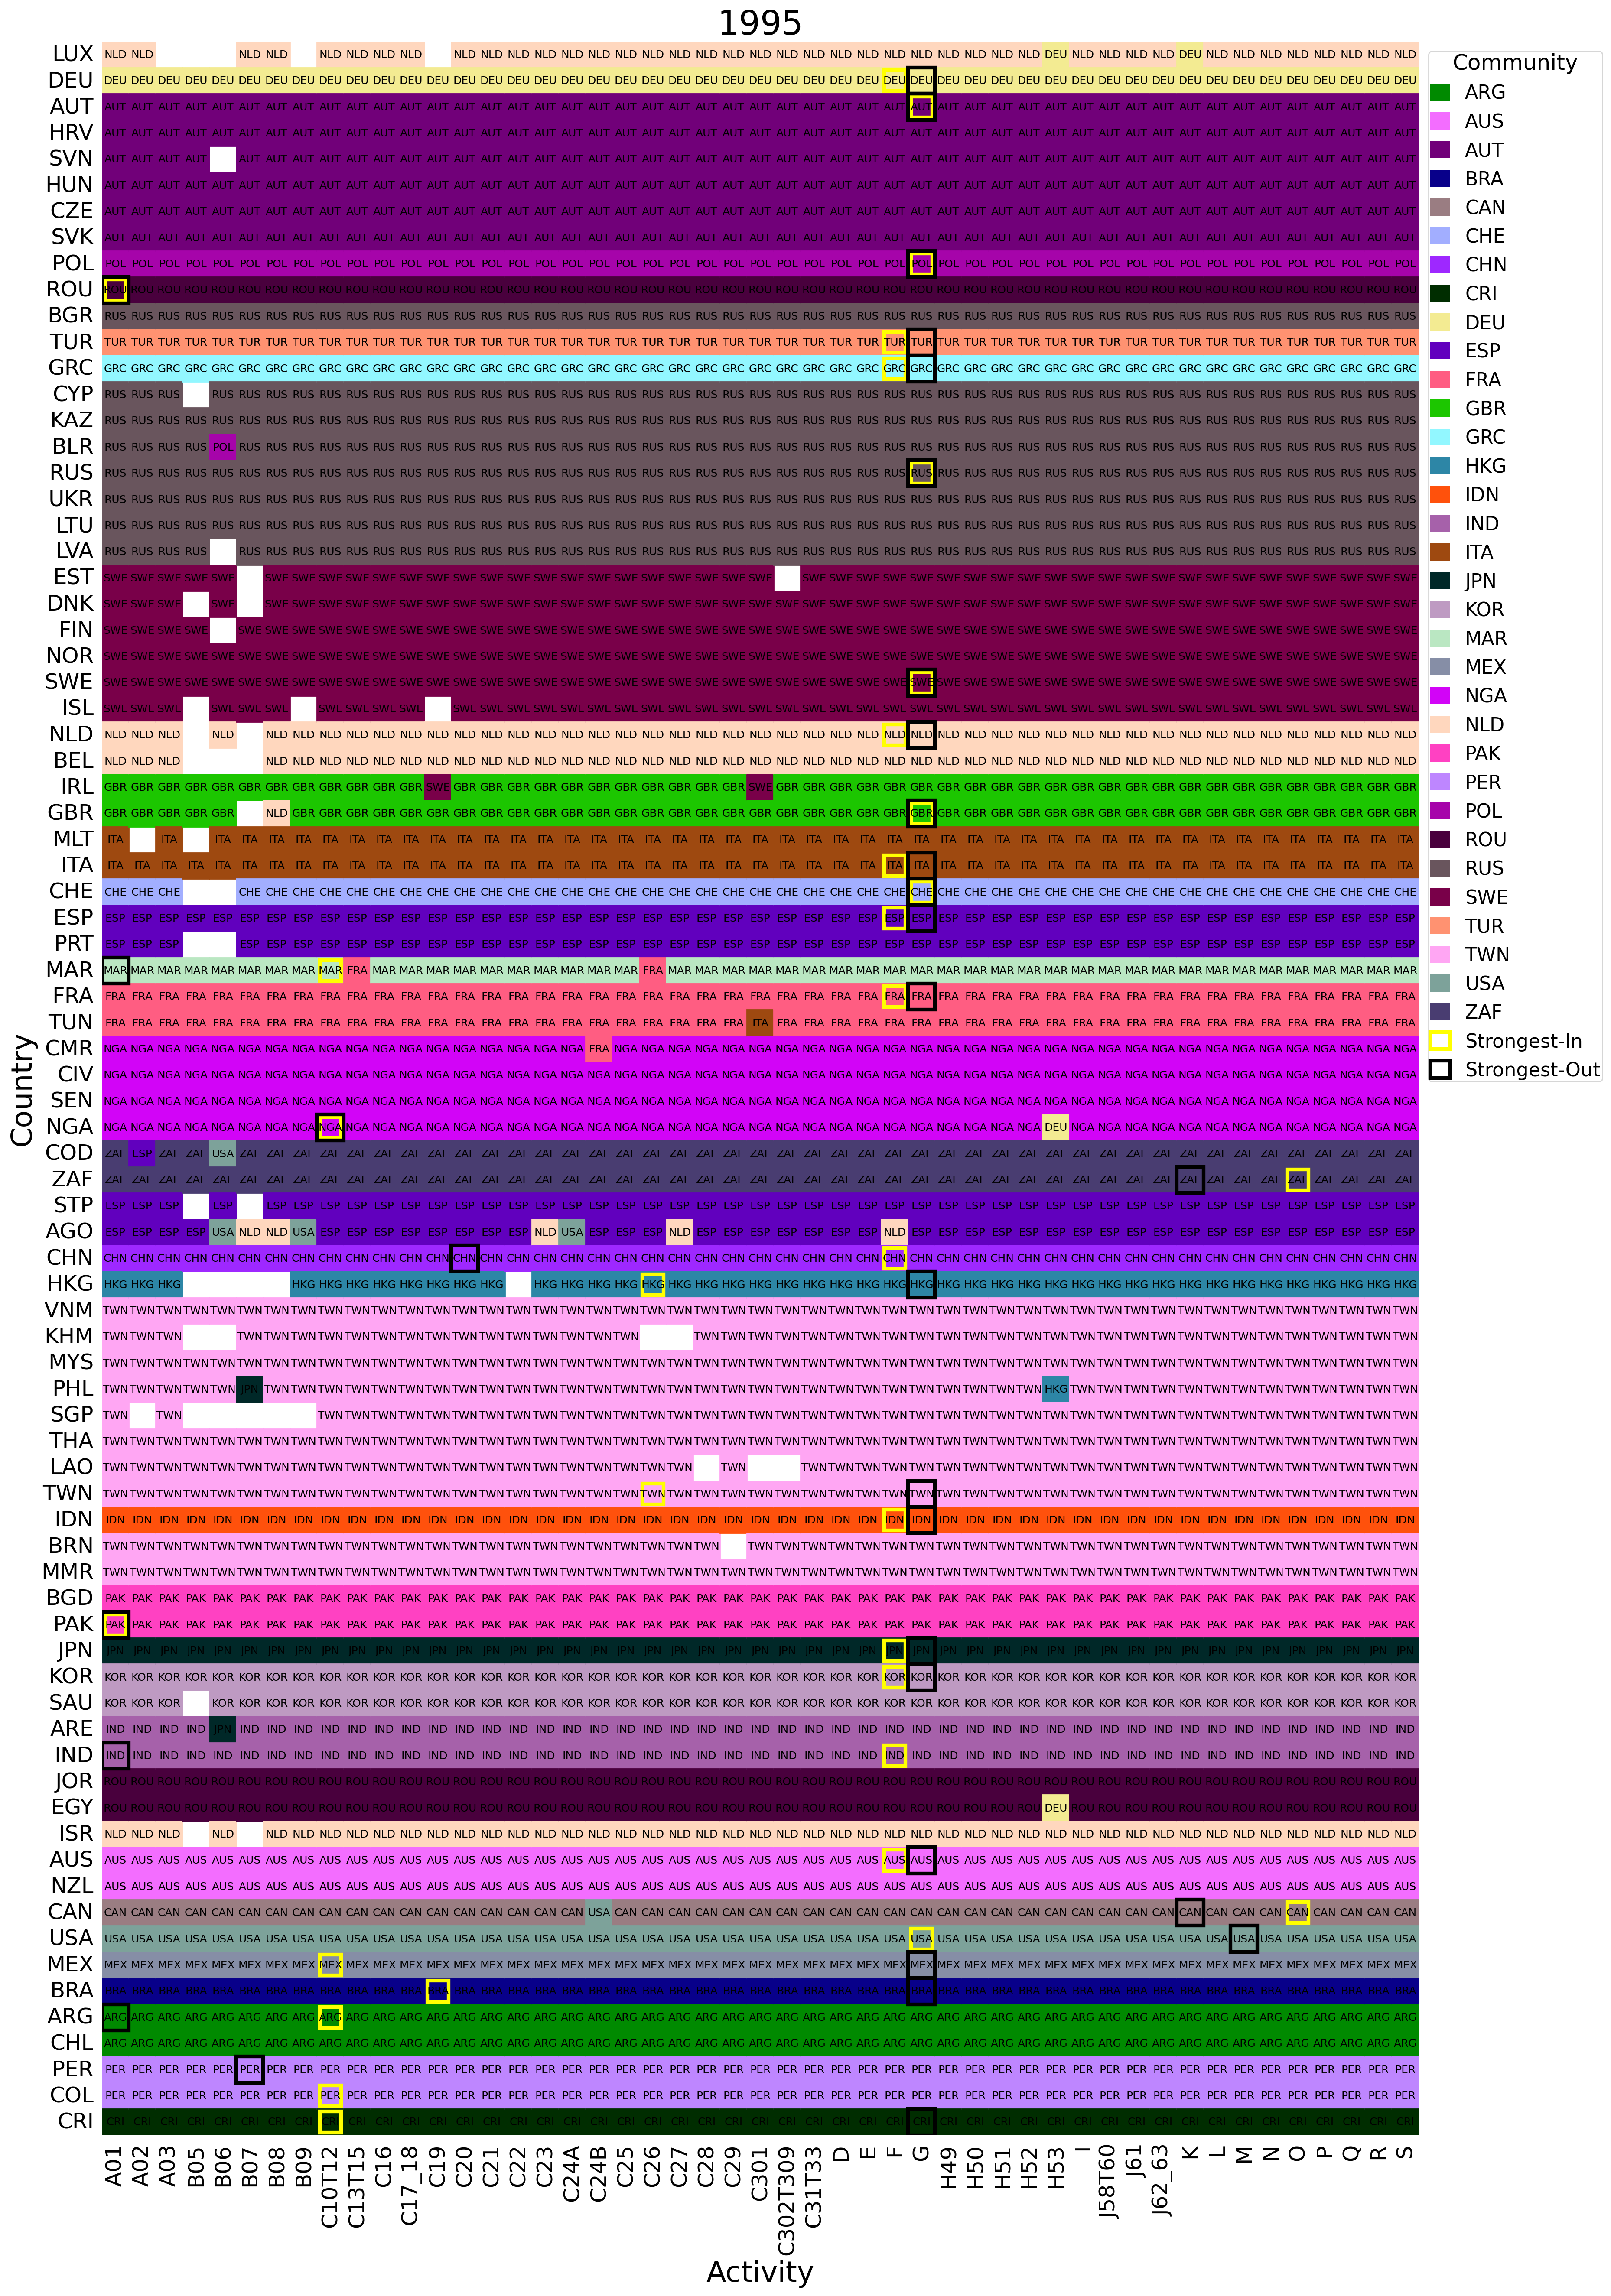
\includegraphics[width=\linewidth]{1995_communities.png}
	\caption{Resultados de la detección de comunidades en 1995.}
	\label{Fig_1995_comunidades}
\end{figure}

\begin{figure}[H]
	\centering
	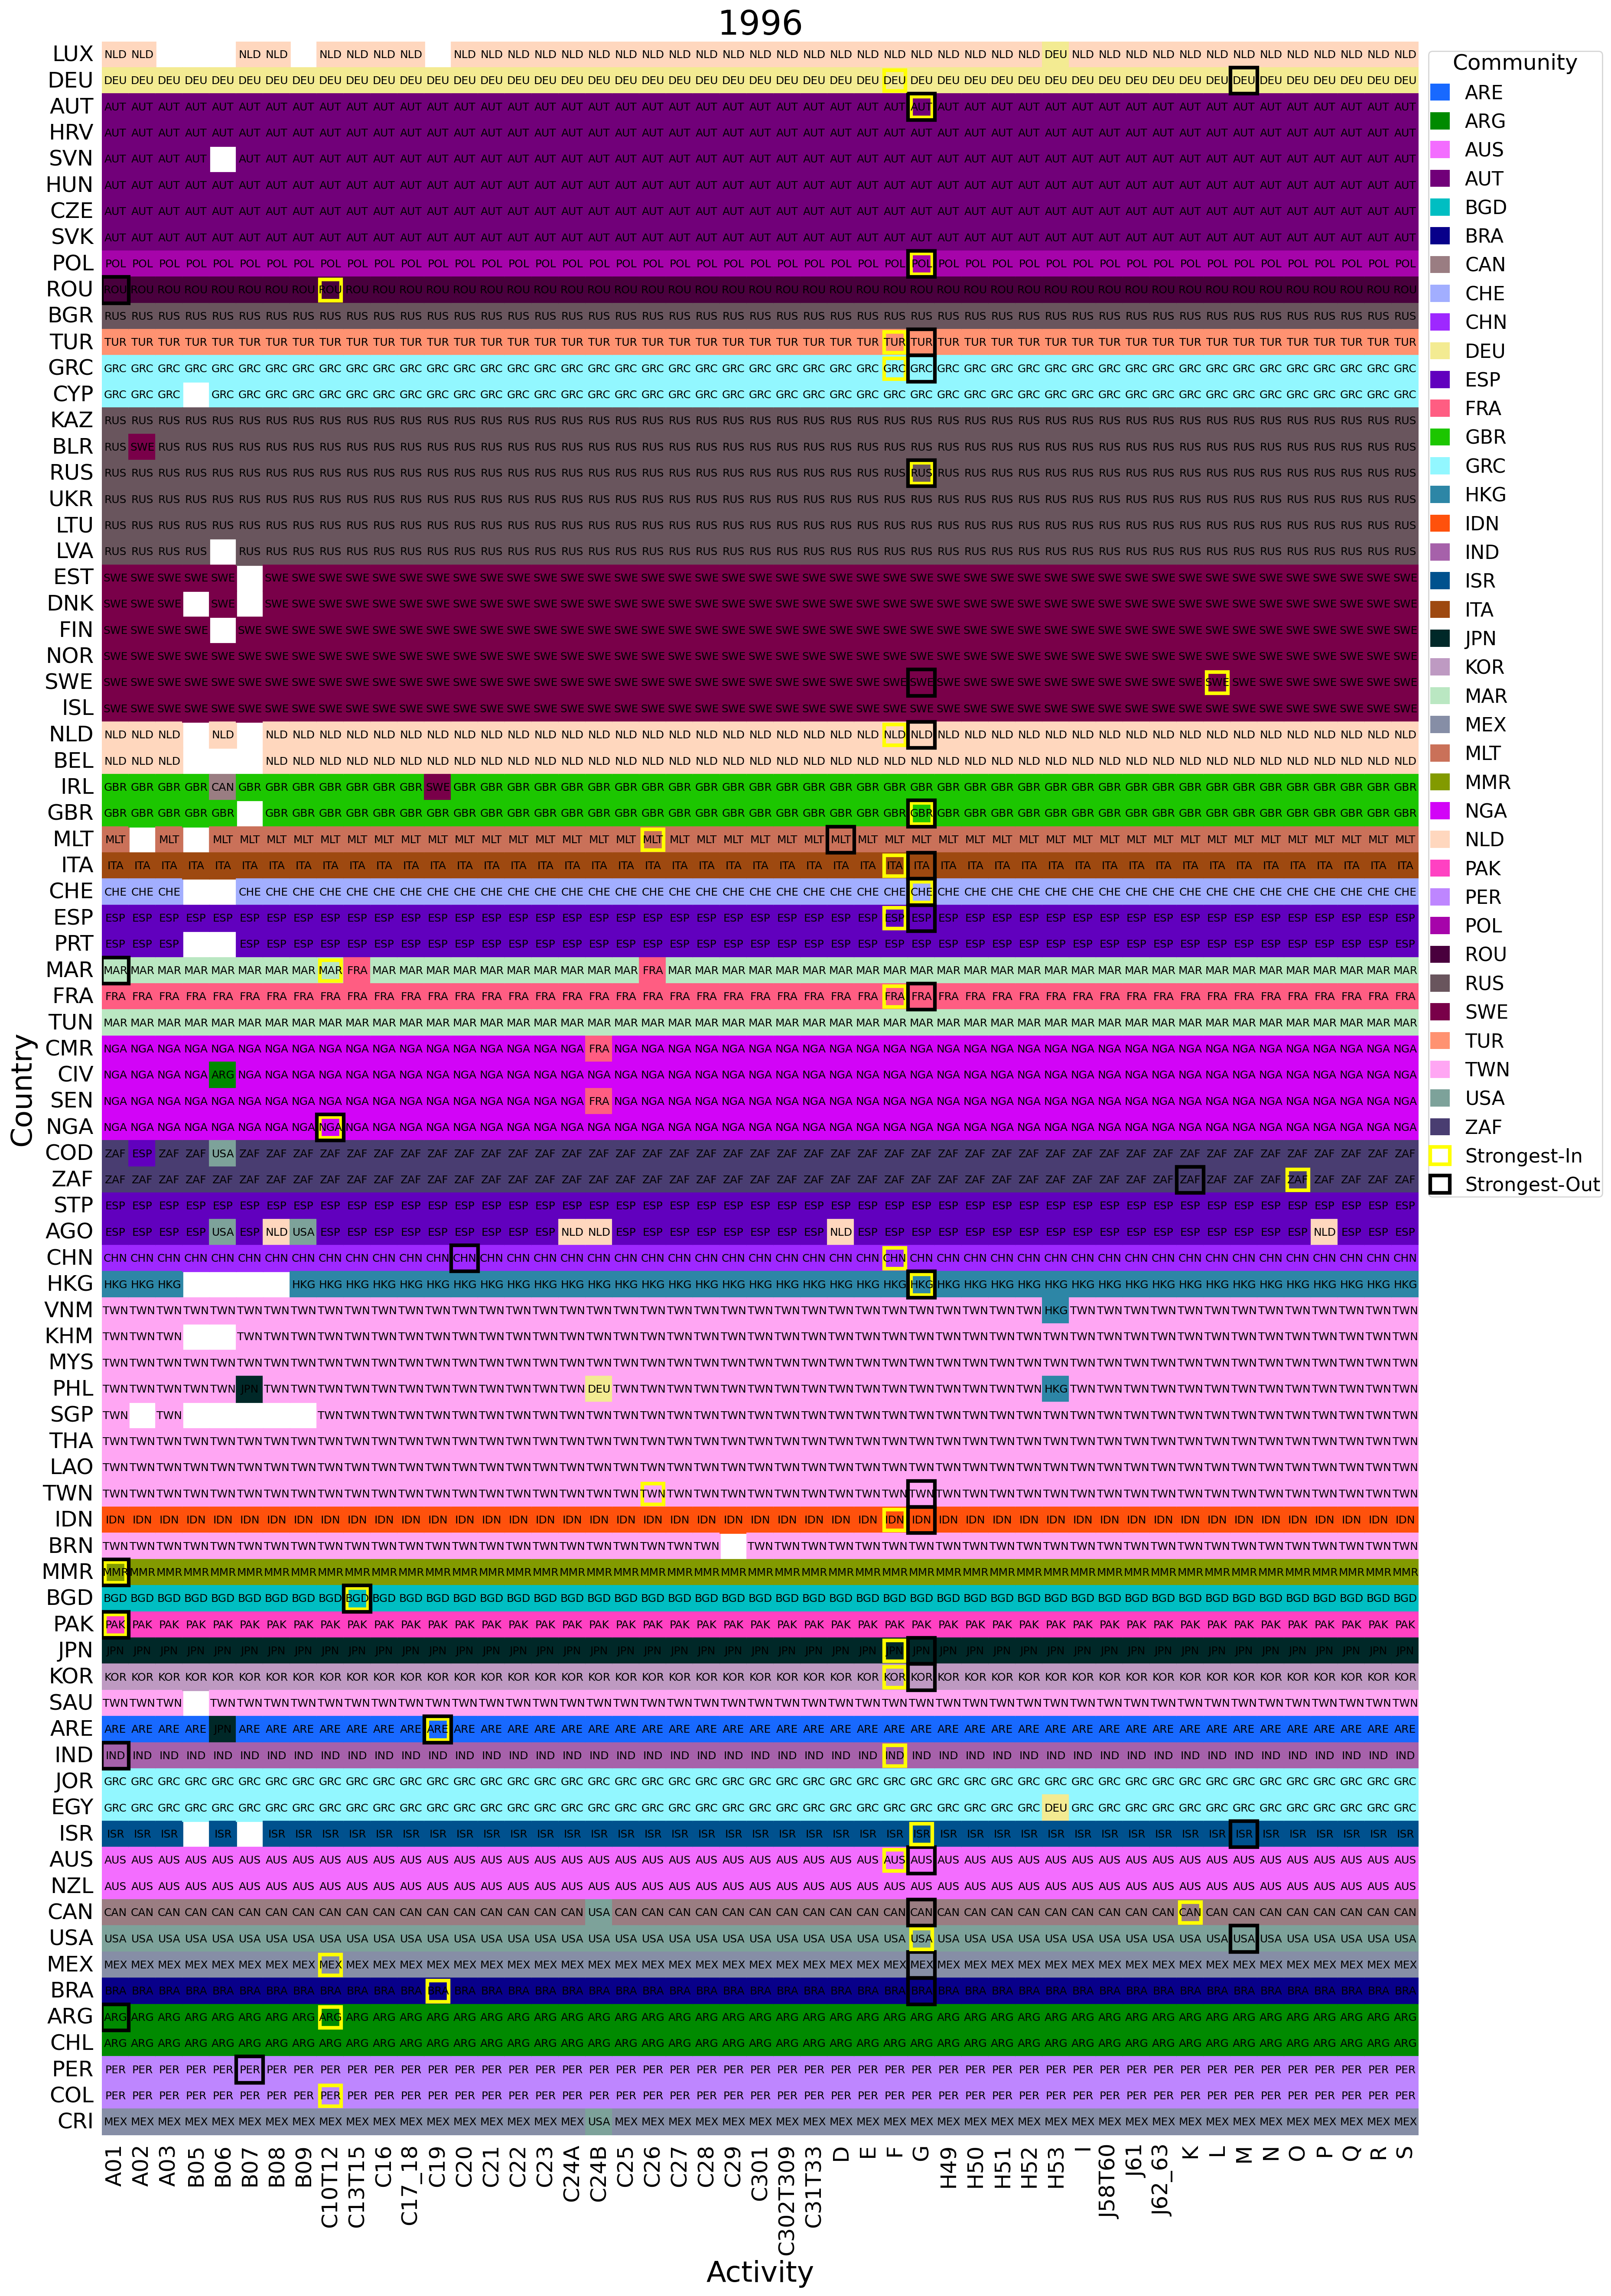
\includegraphics[width=\linewidth]{1996_communities.png}
	\caption{Resultados de la detección de comunidades en 1996.}
	\label{Fig_1996_comunidades}
\end{figure}

\begin{figure}[H]
	\centering
	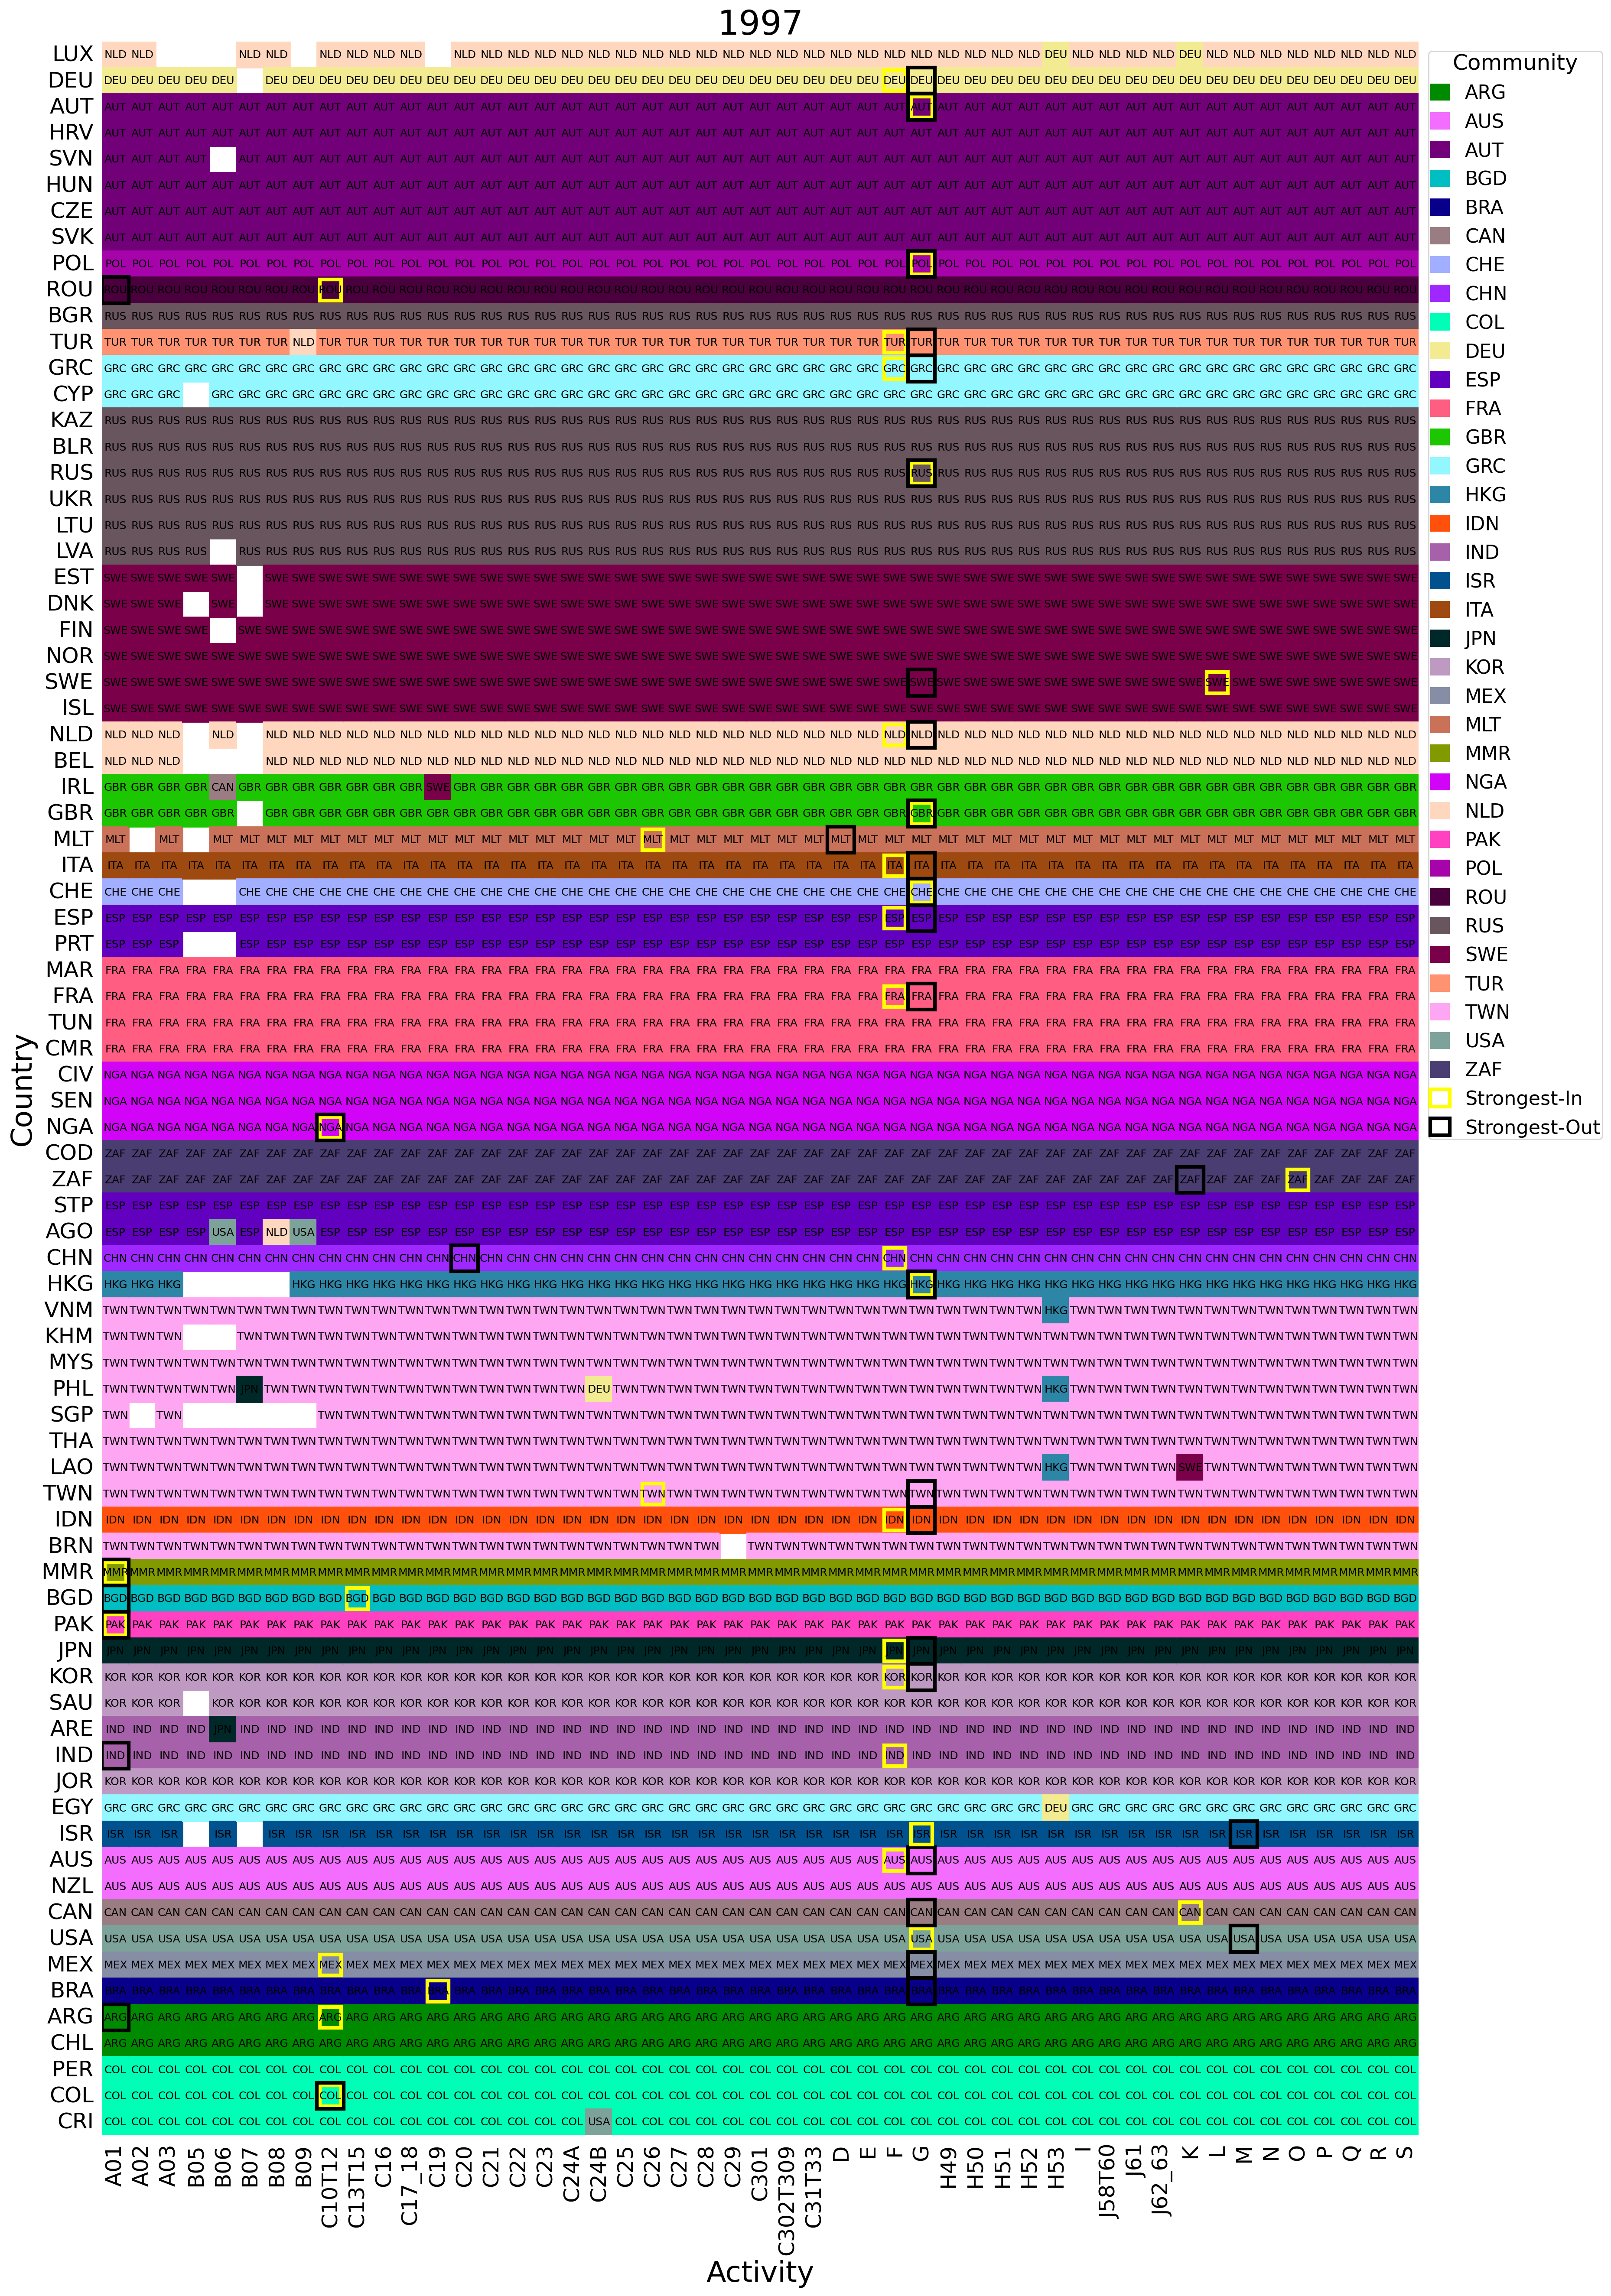
\includegraphics[width=\linewidth]{1997_communities.png}
	\caption{Resultados de la detección de comunidades en 1997.}
	\label{Fig_1997_comunidades}
\end{figure}

\begin{figure}[H]
	\centering
	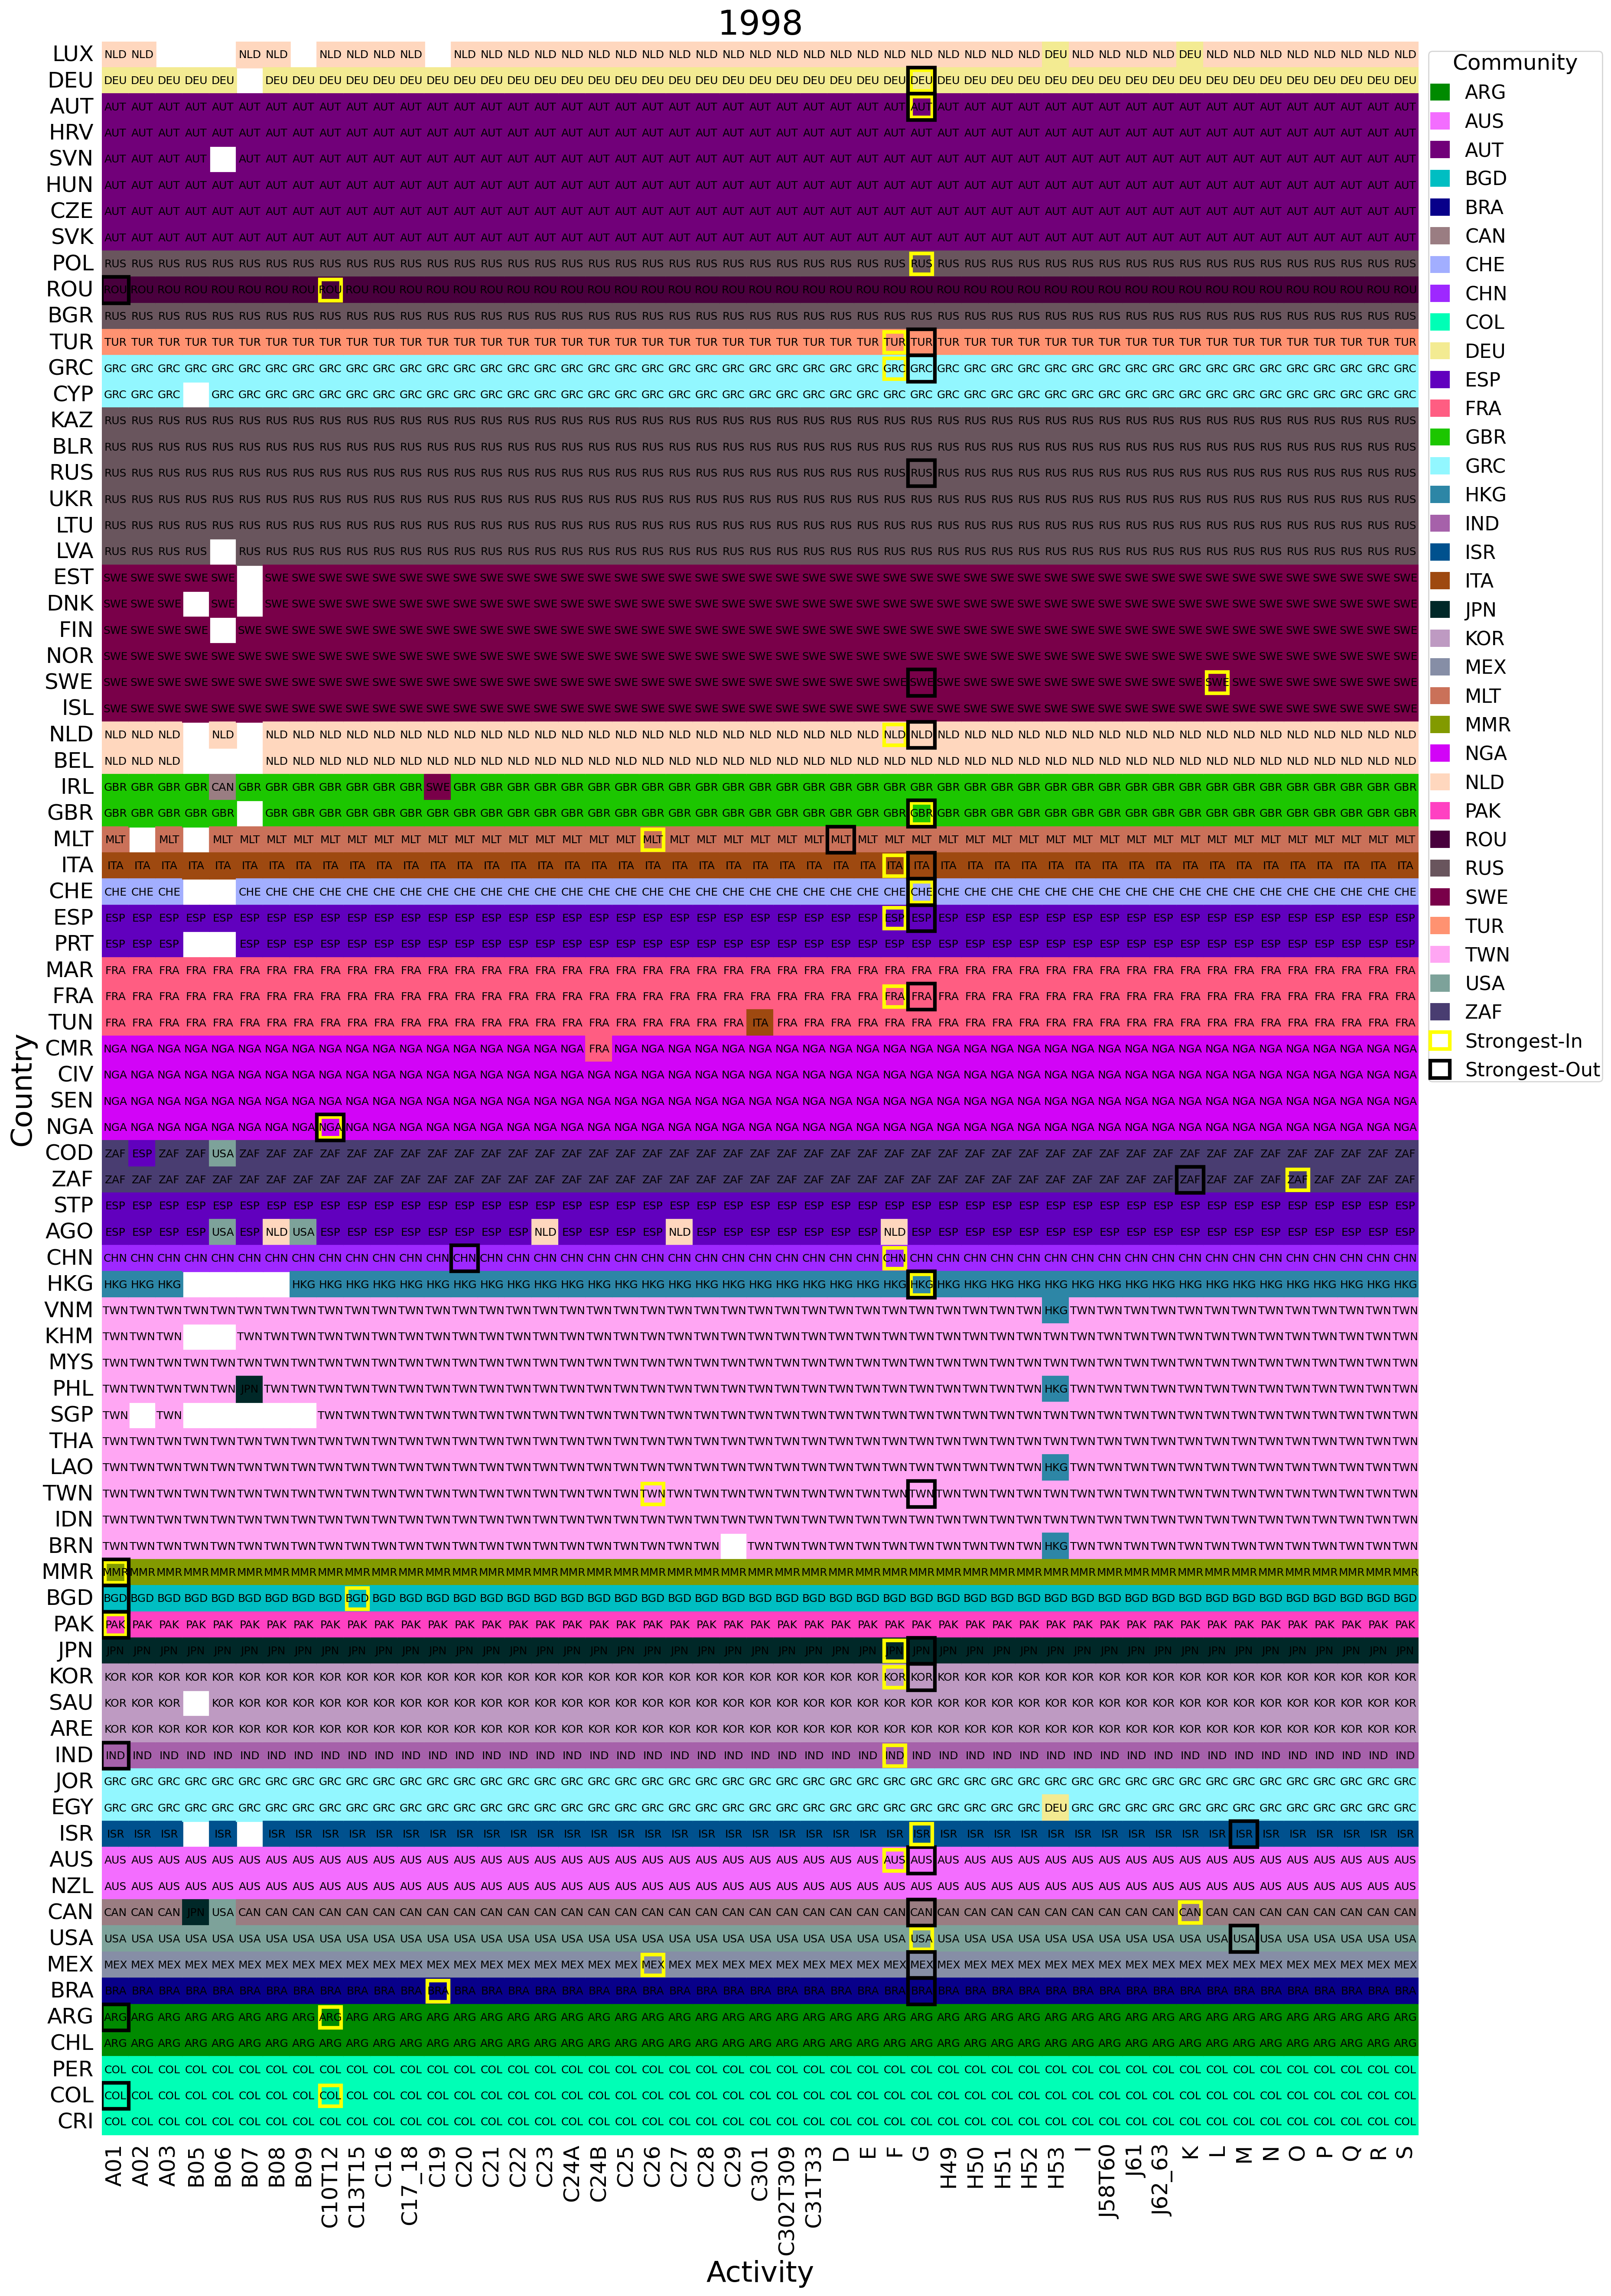
\includegraphics[width=\linewidth]{1998_communities.png}
	\caption{Resultados de la detección de comunidades en 1998.}
	\label{Fig_1998_comunidades}
\end{figure}

\begin{figure}[H]
	\centering
	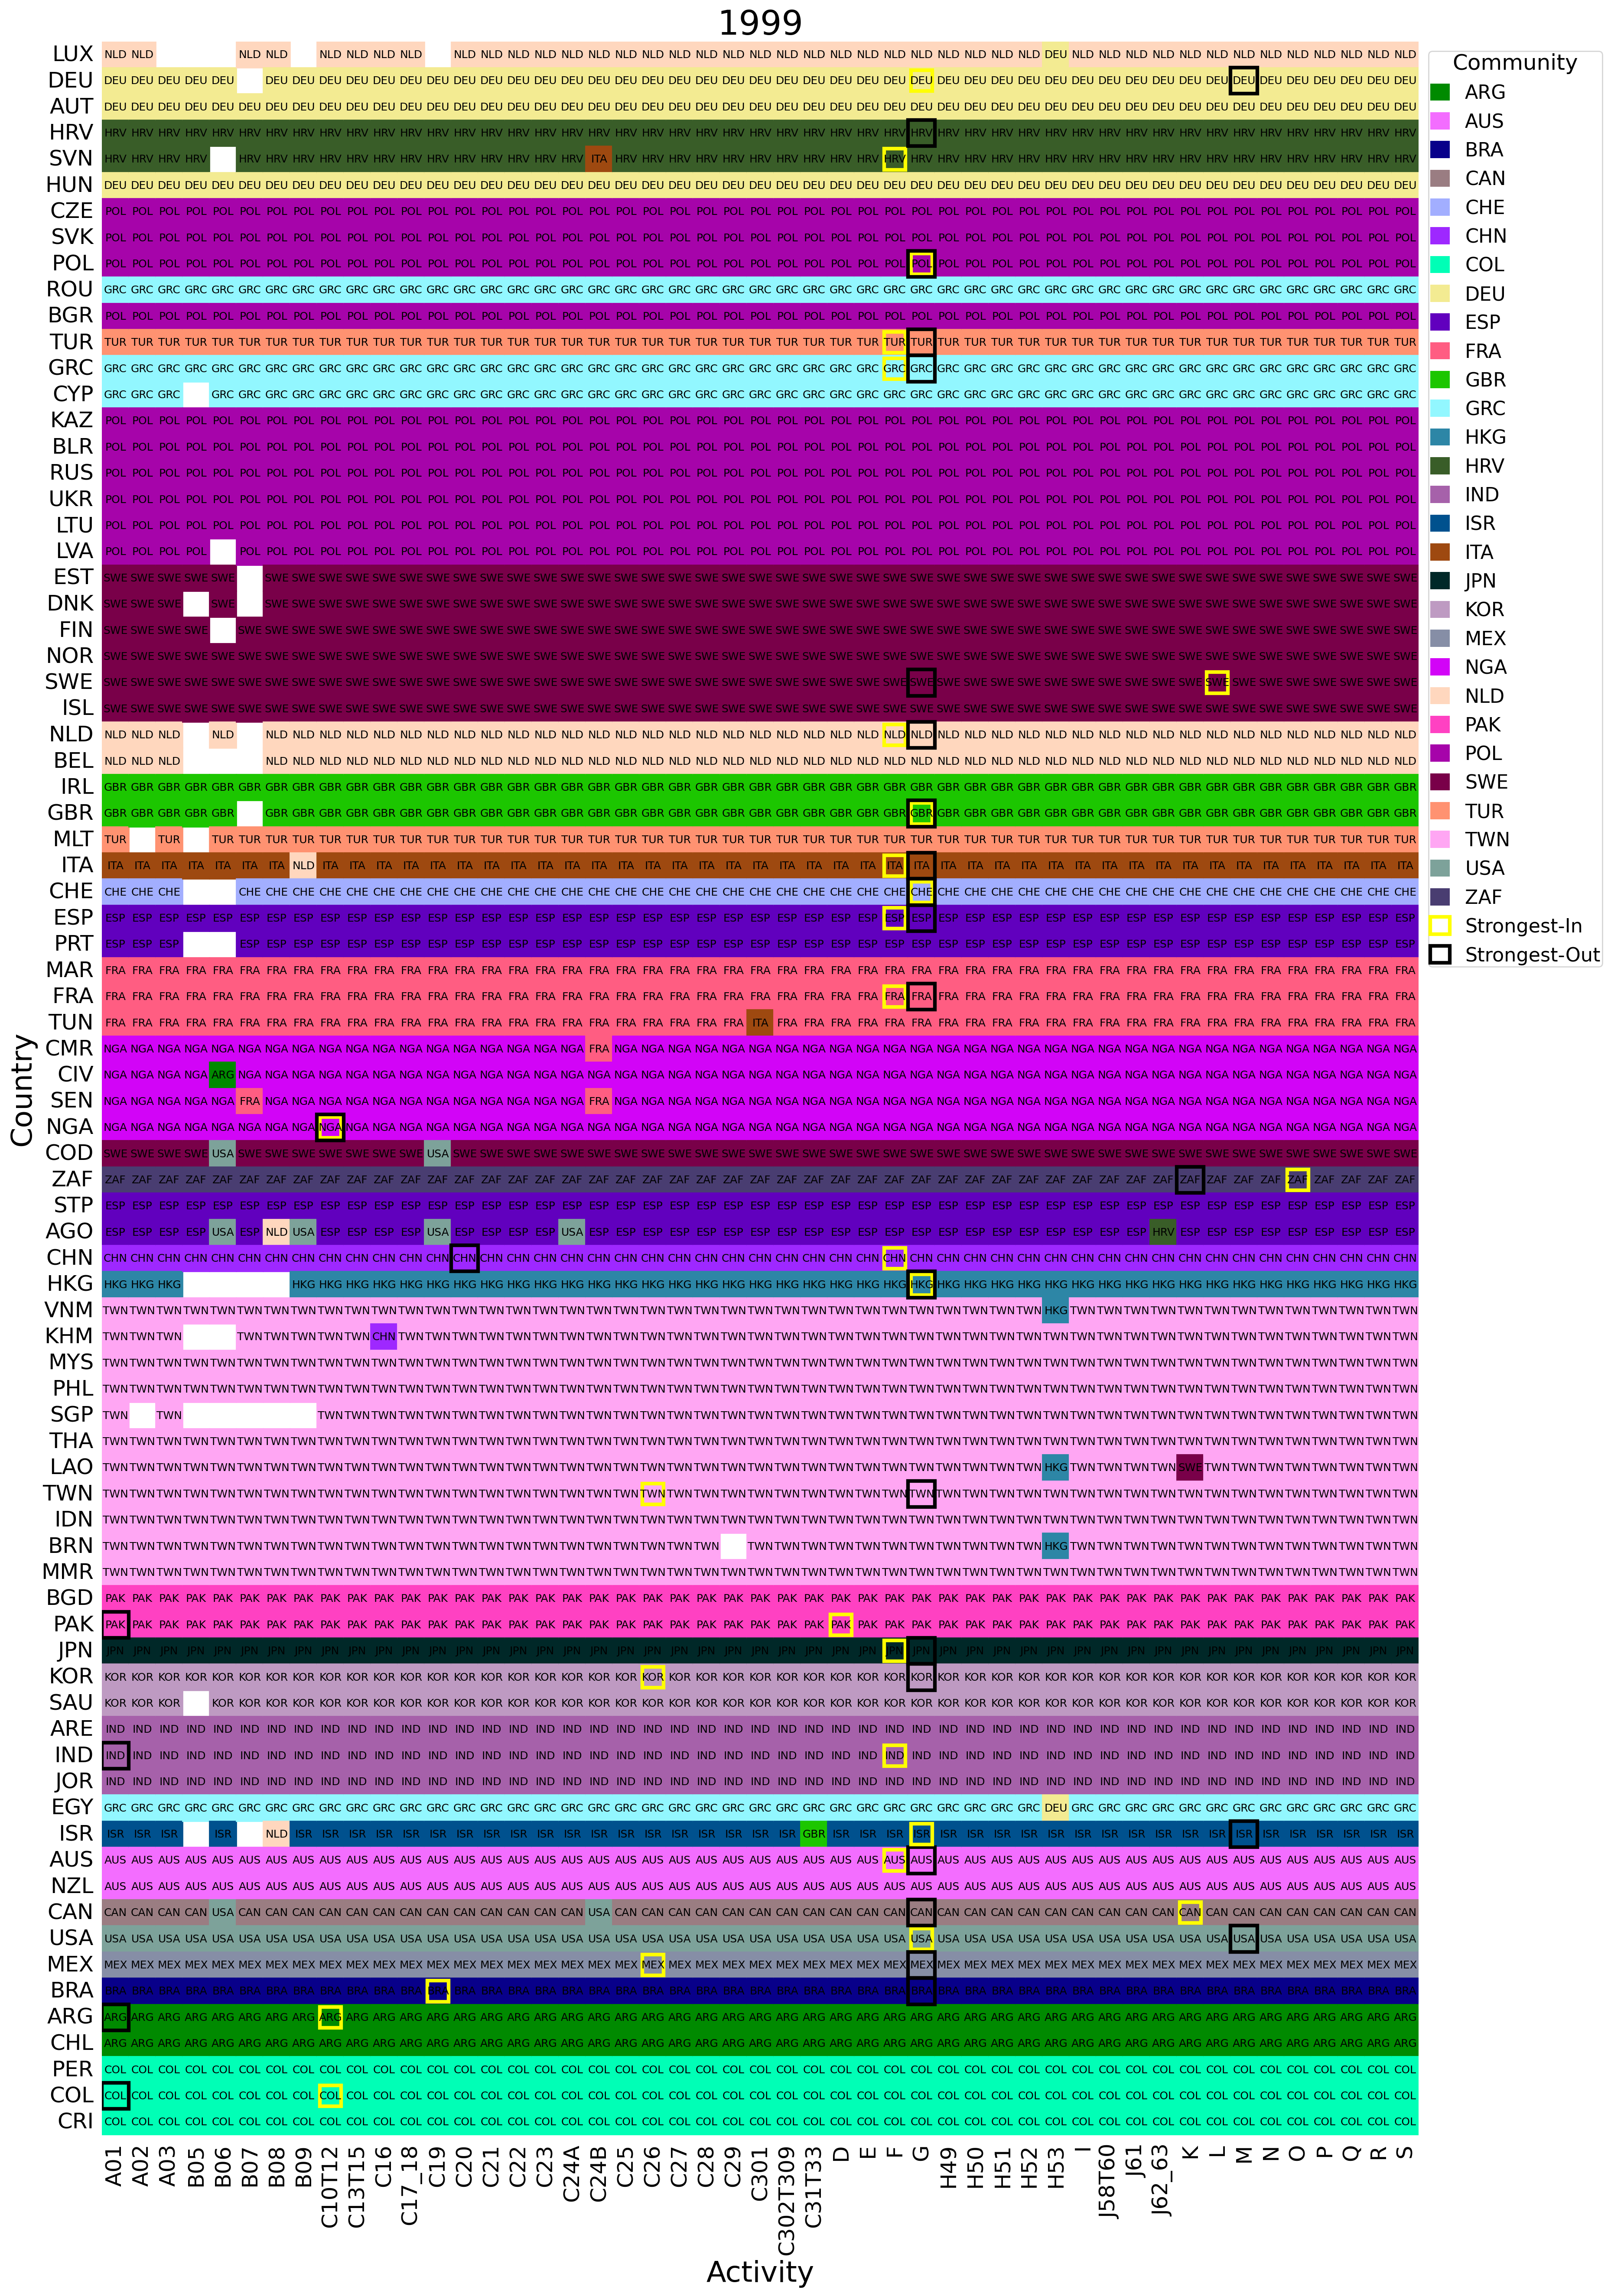
\includegraphics[width=\linewidth]{1999_communities.png}
	\caption{Resultados de la detección de comunidades en 1999.}
	\label{Fig_1999_comunidades}
\end{figure}

\begin{figure}[H]
	\centering
	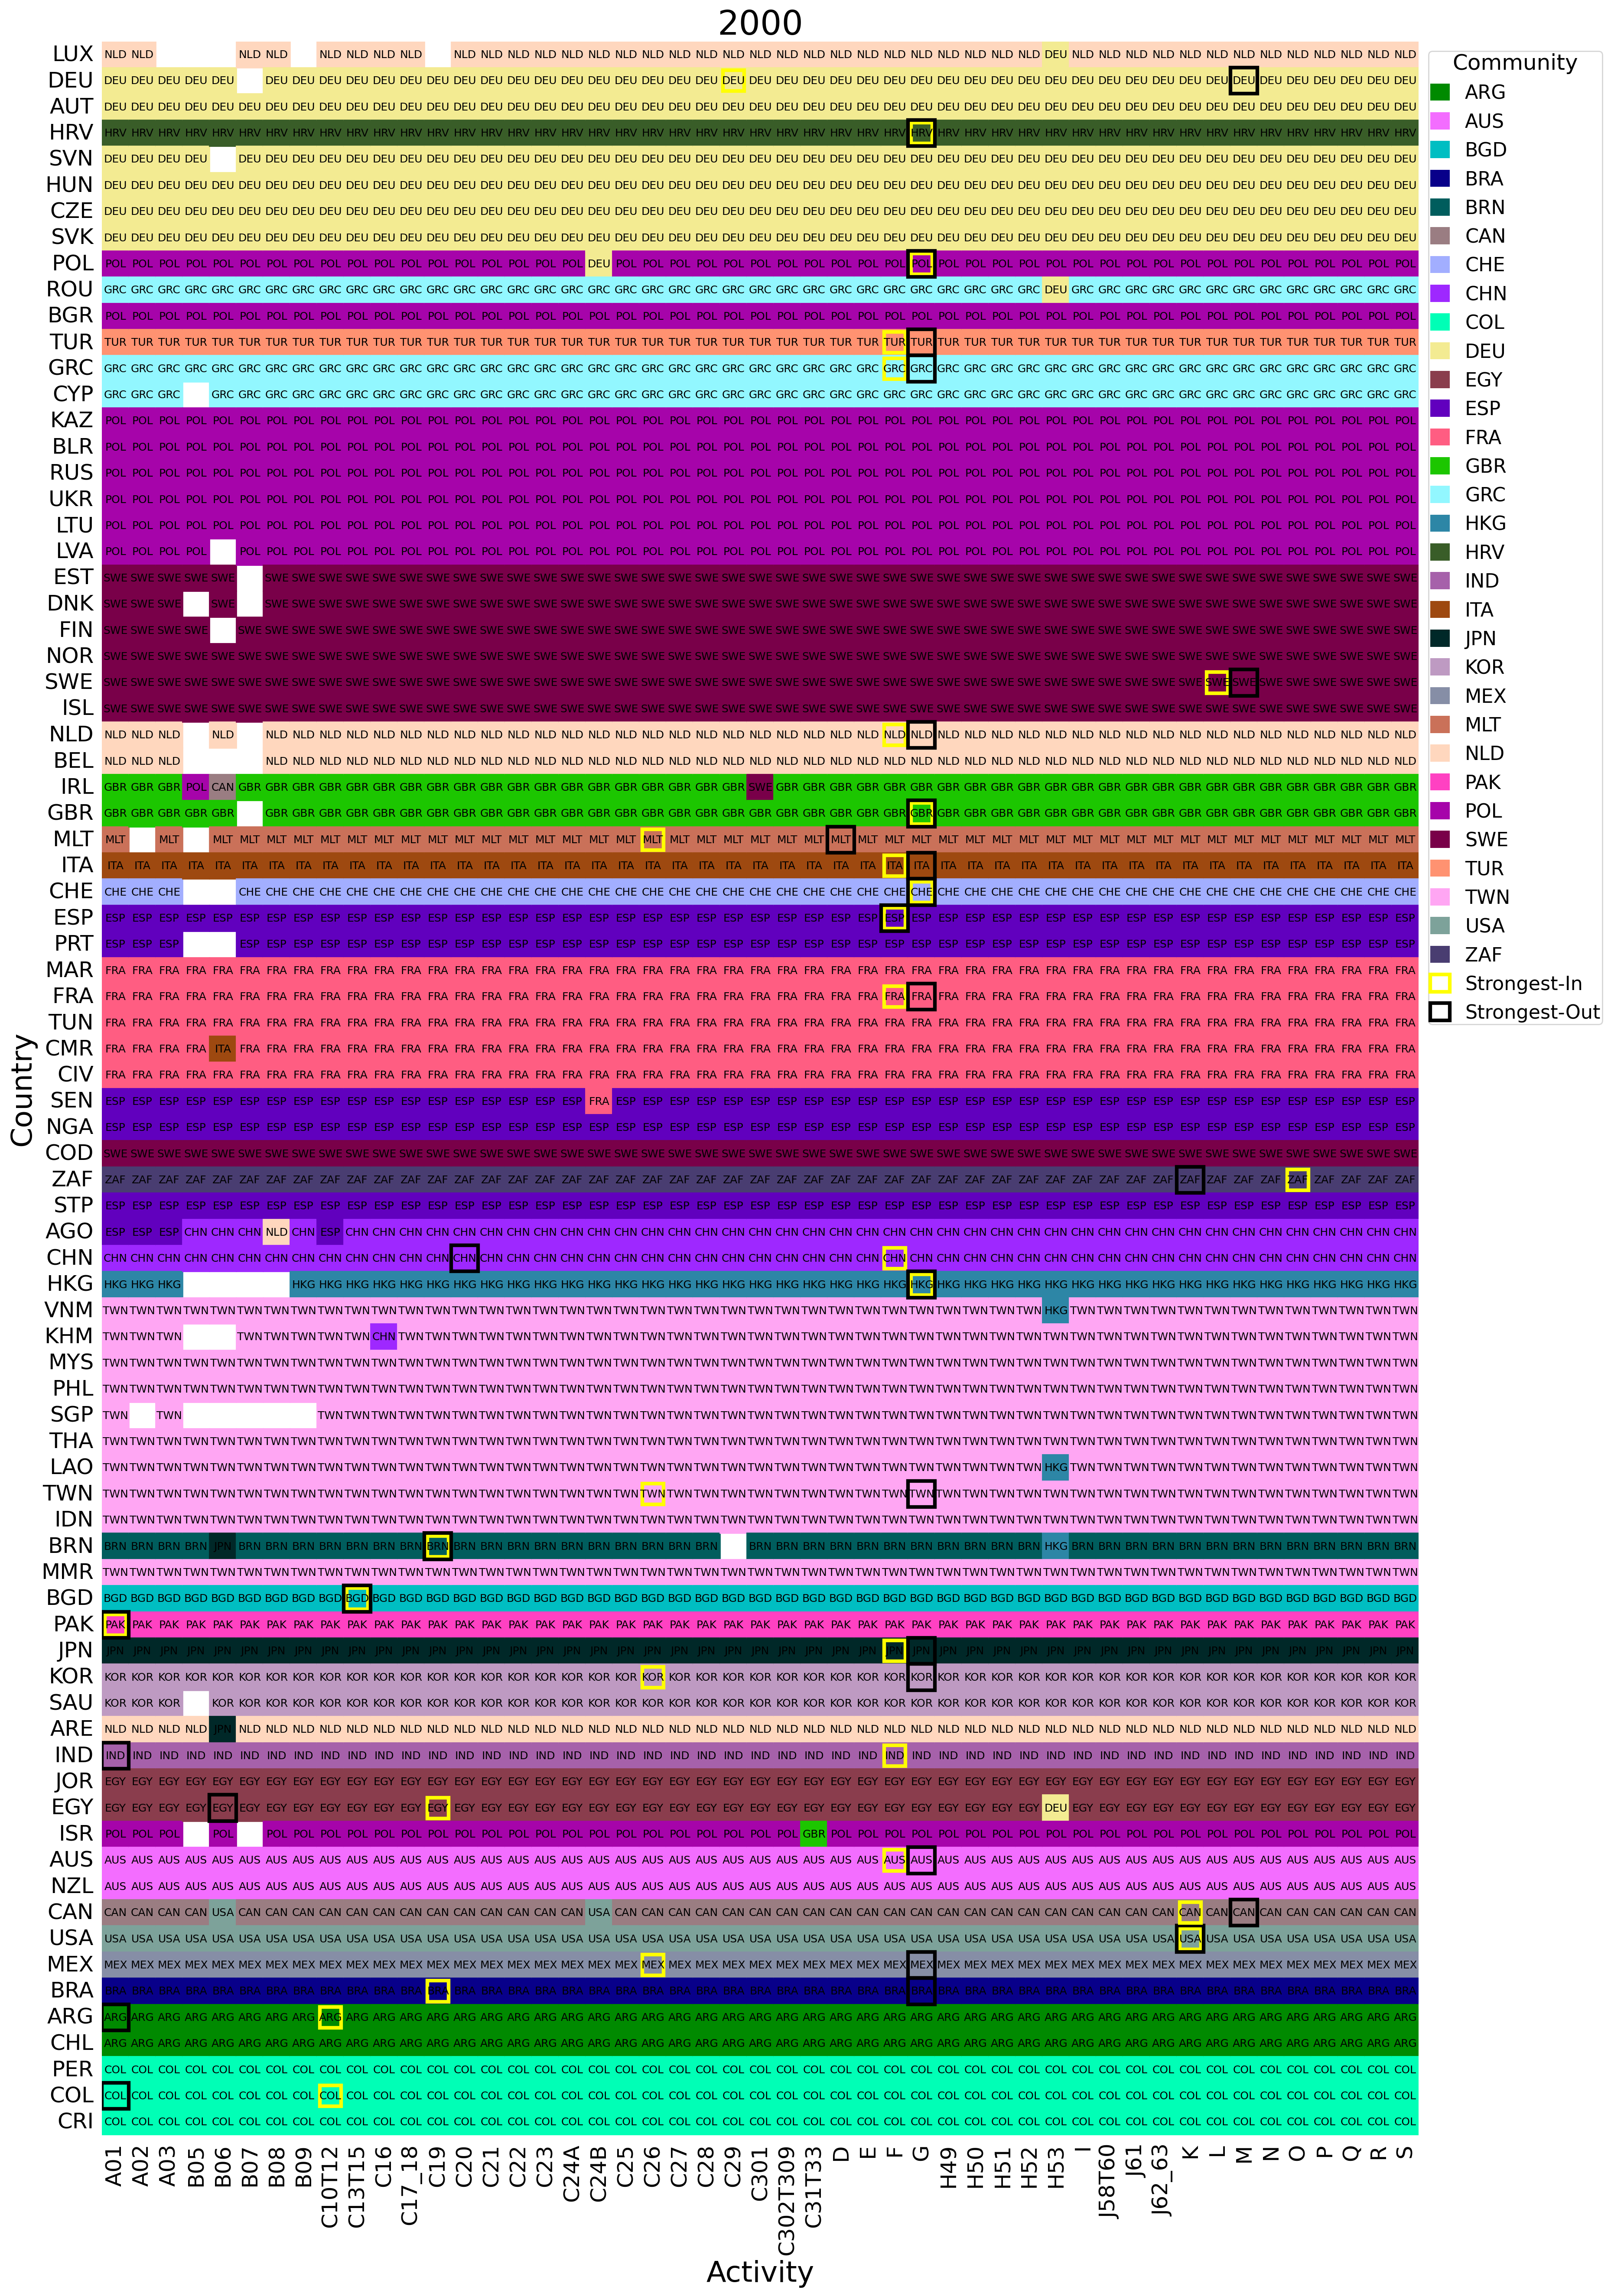
\includegraphics[width=\linewidth]{2000_communities.png}
	\caption{Resultados de la detección de comunidades en 2000.}
	\label{Fig_2000_comunidades}
\end{figure}

\begin{figure}[H]
	\centering
	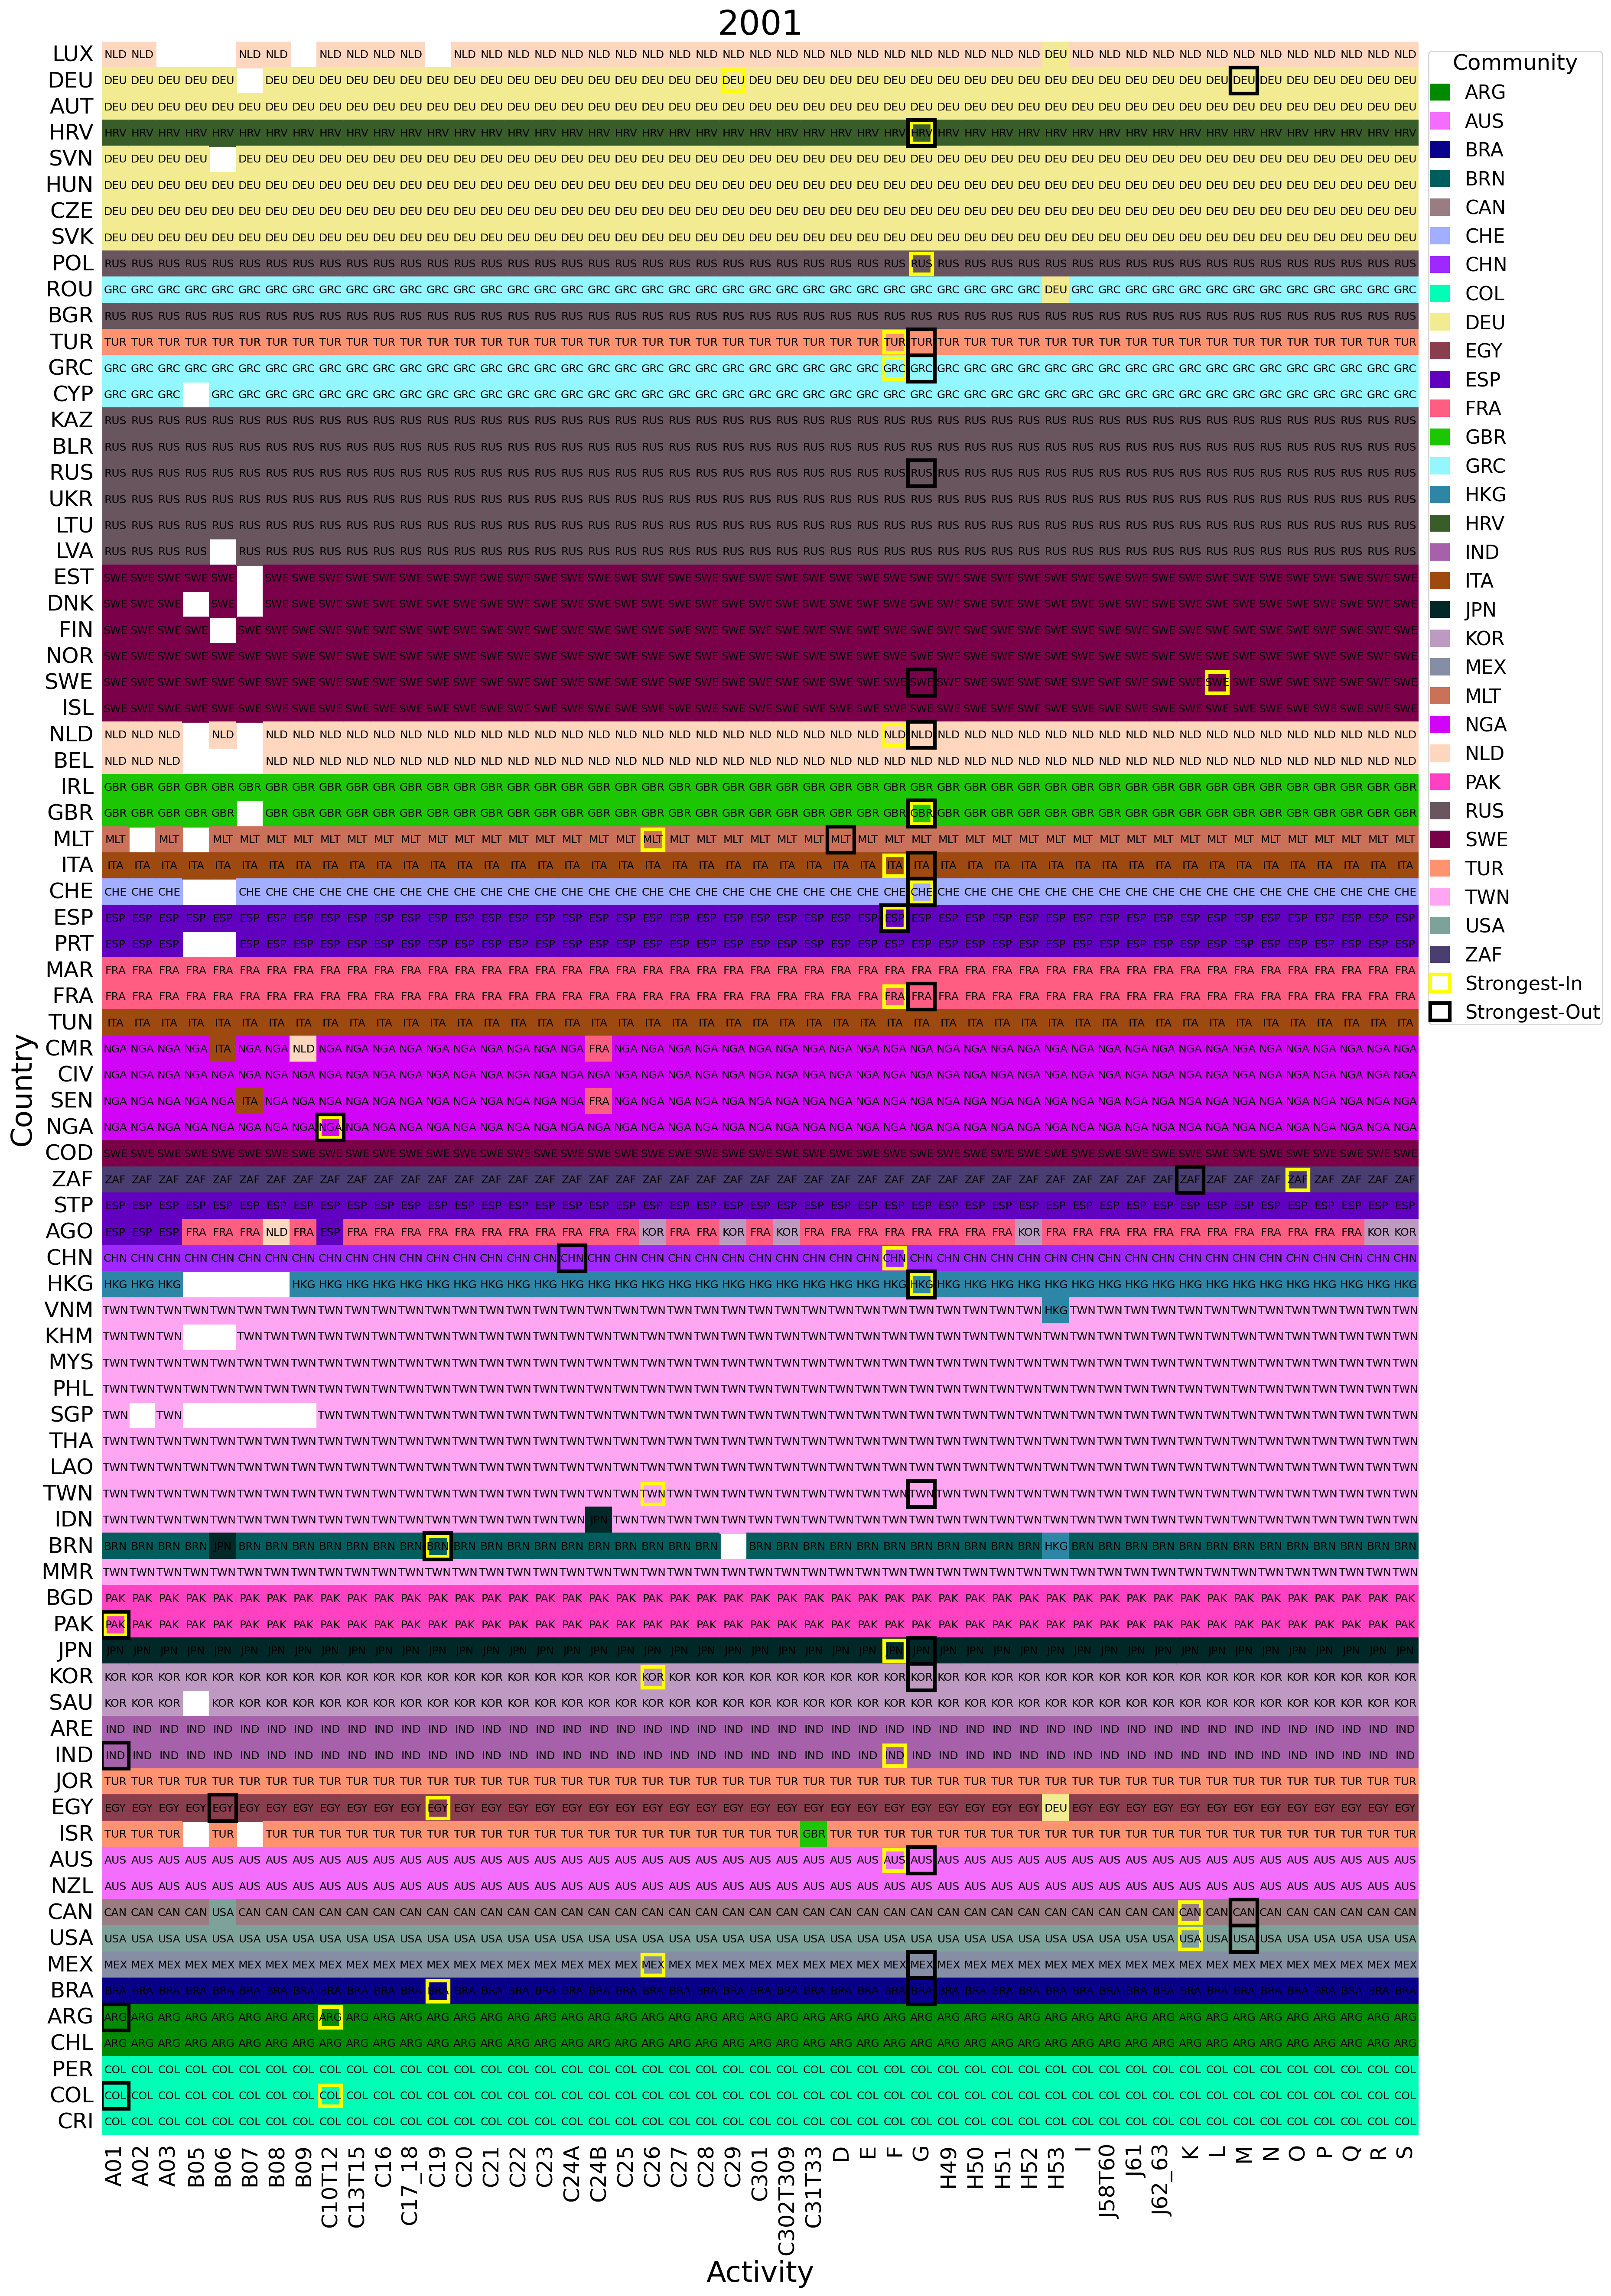
\includegraphics[width=\linewidth]{2001_communities.png}
	\caption{Resultados de la detección de comunidades en 2001.}
	\label{Fig_2001_comunidades}
\end{figure}

\begin{figure}[H]
	\centering
	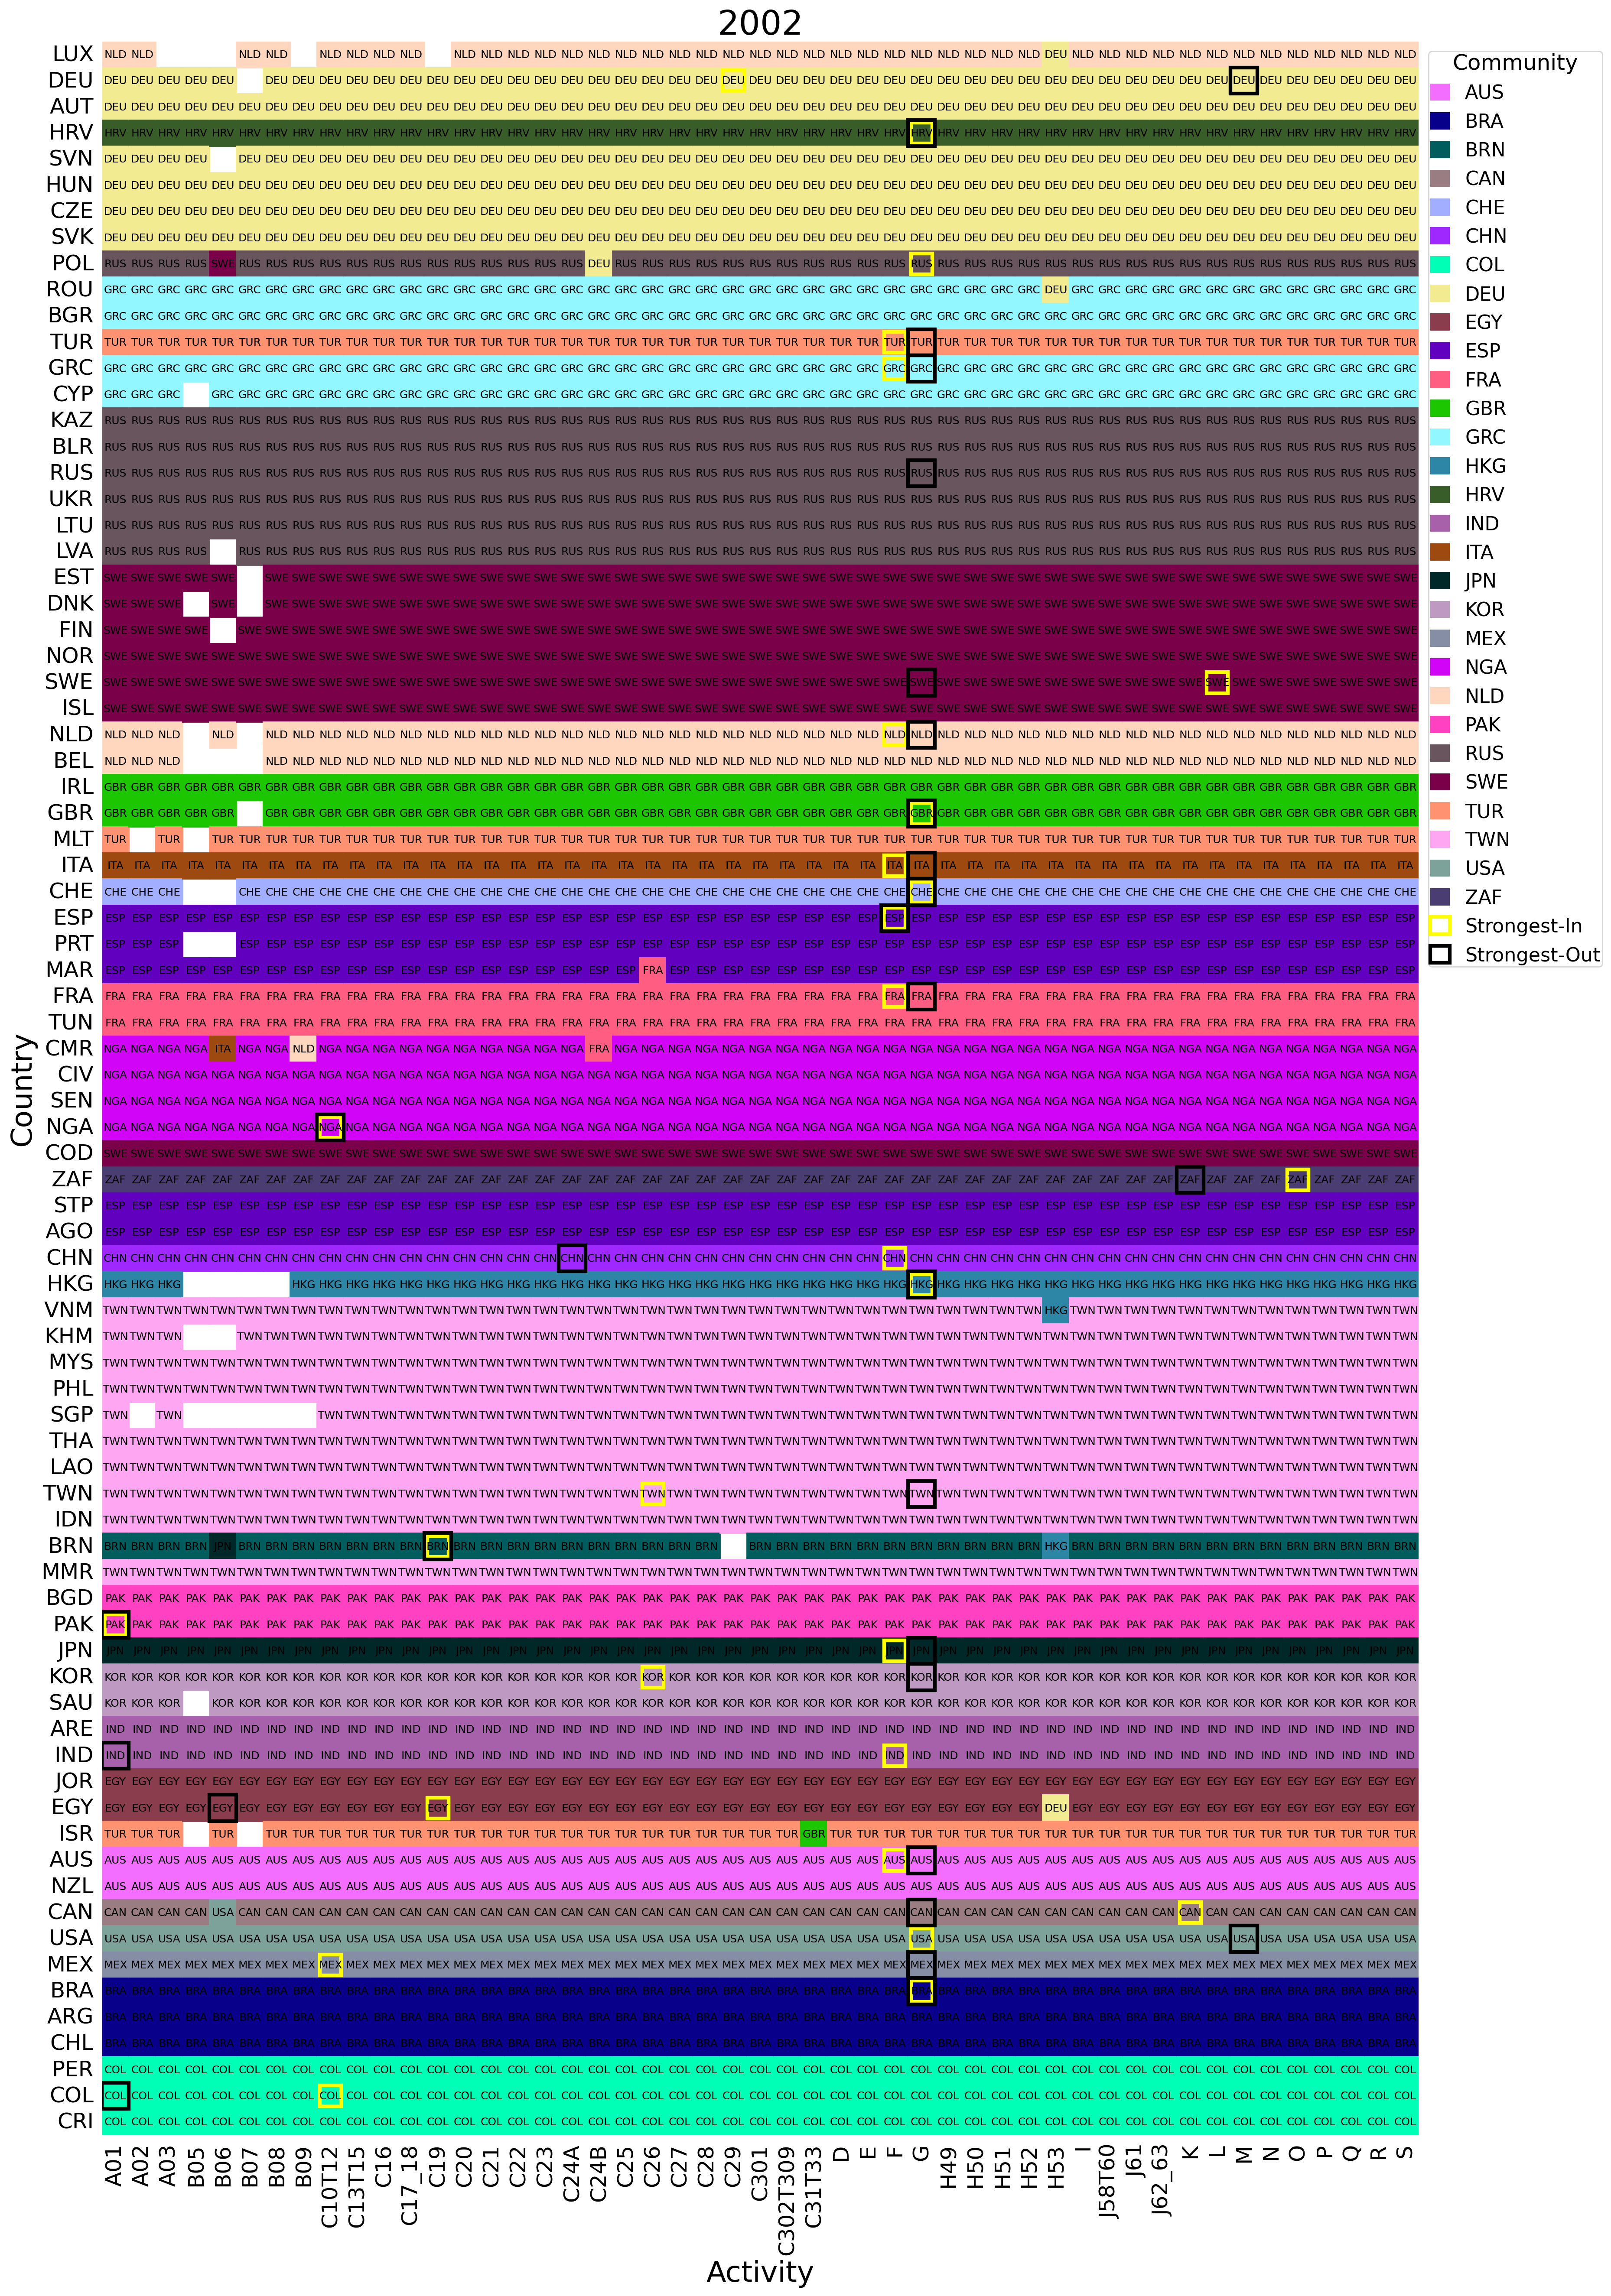
\includegraphics[width=\linewidth]{2002_communities.png}
	\caption{Resultados de la detección de comunidades en 2002.}
	\label{Fig_2002_comunidades}
\end{figure}

\begin{figure}[H]
	\centering
	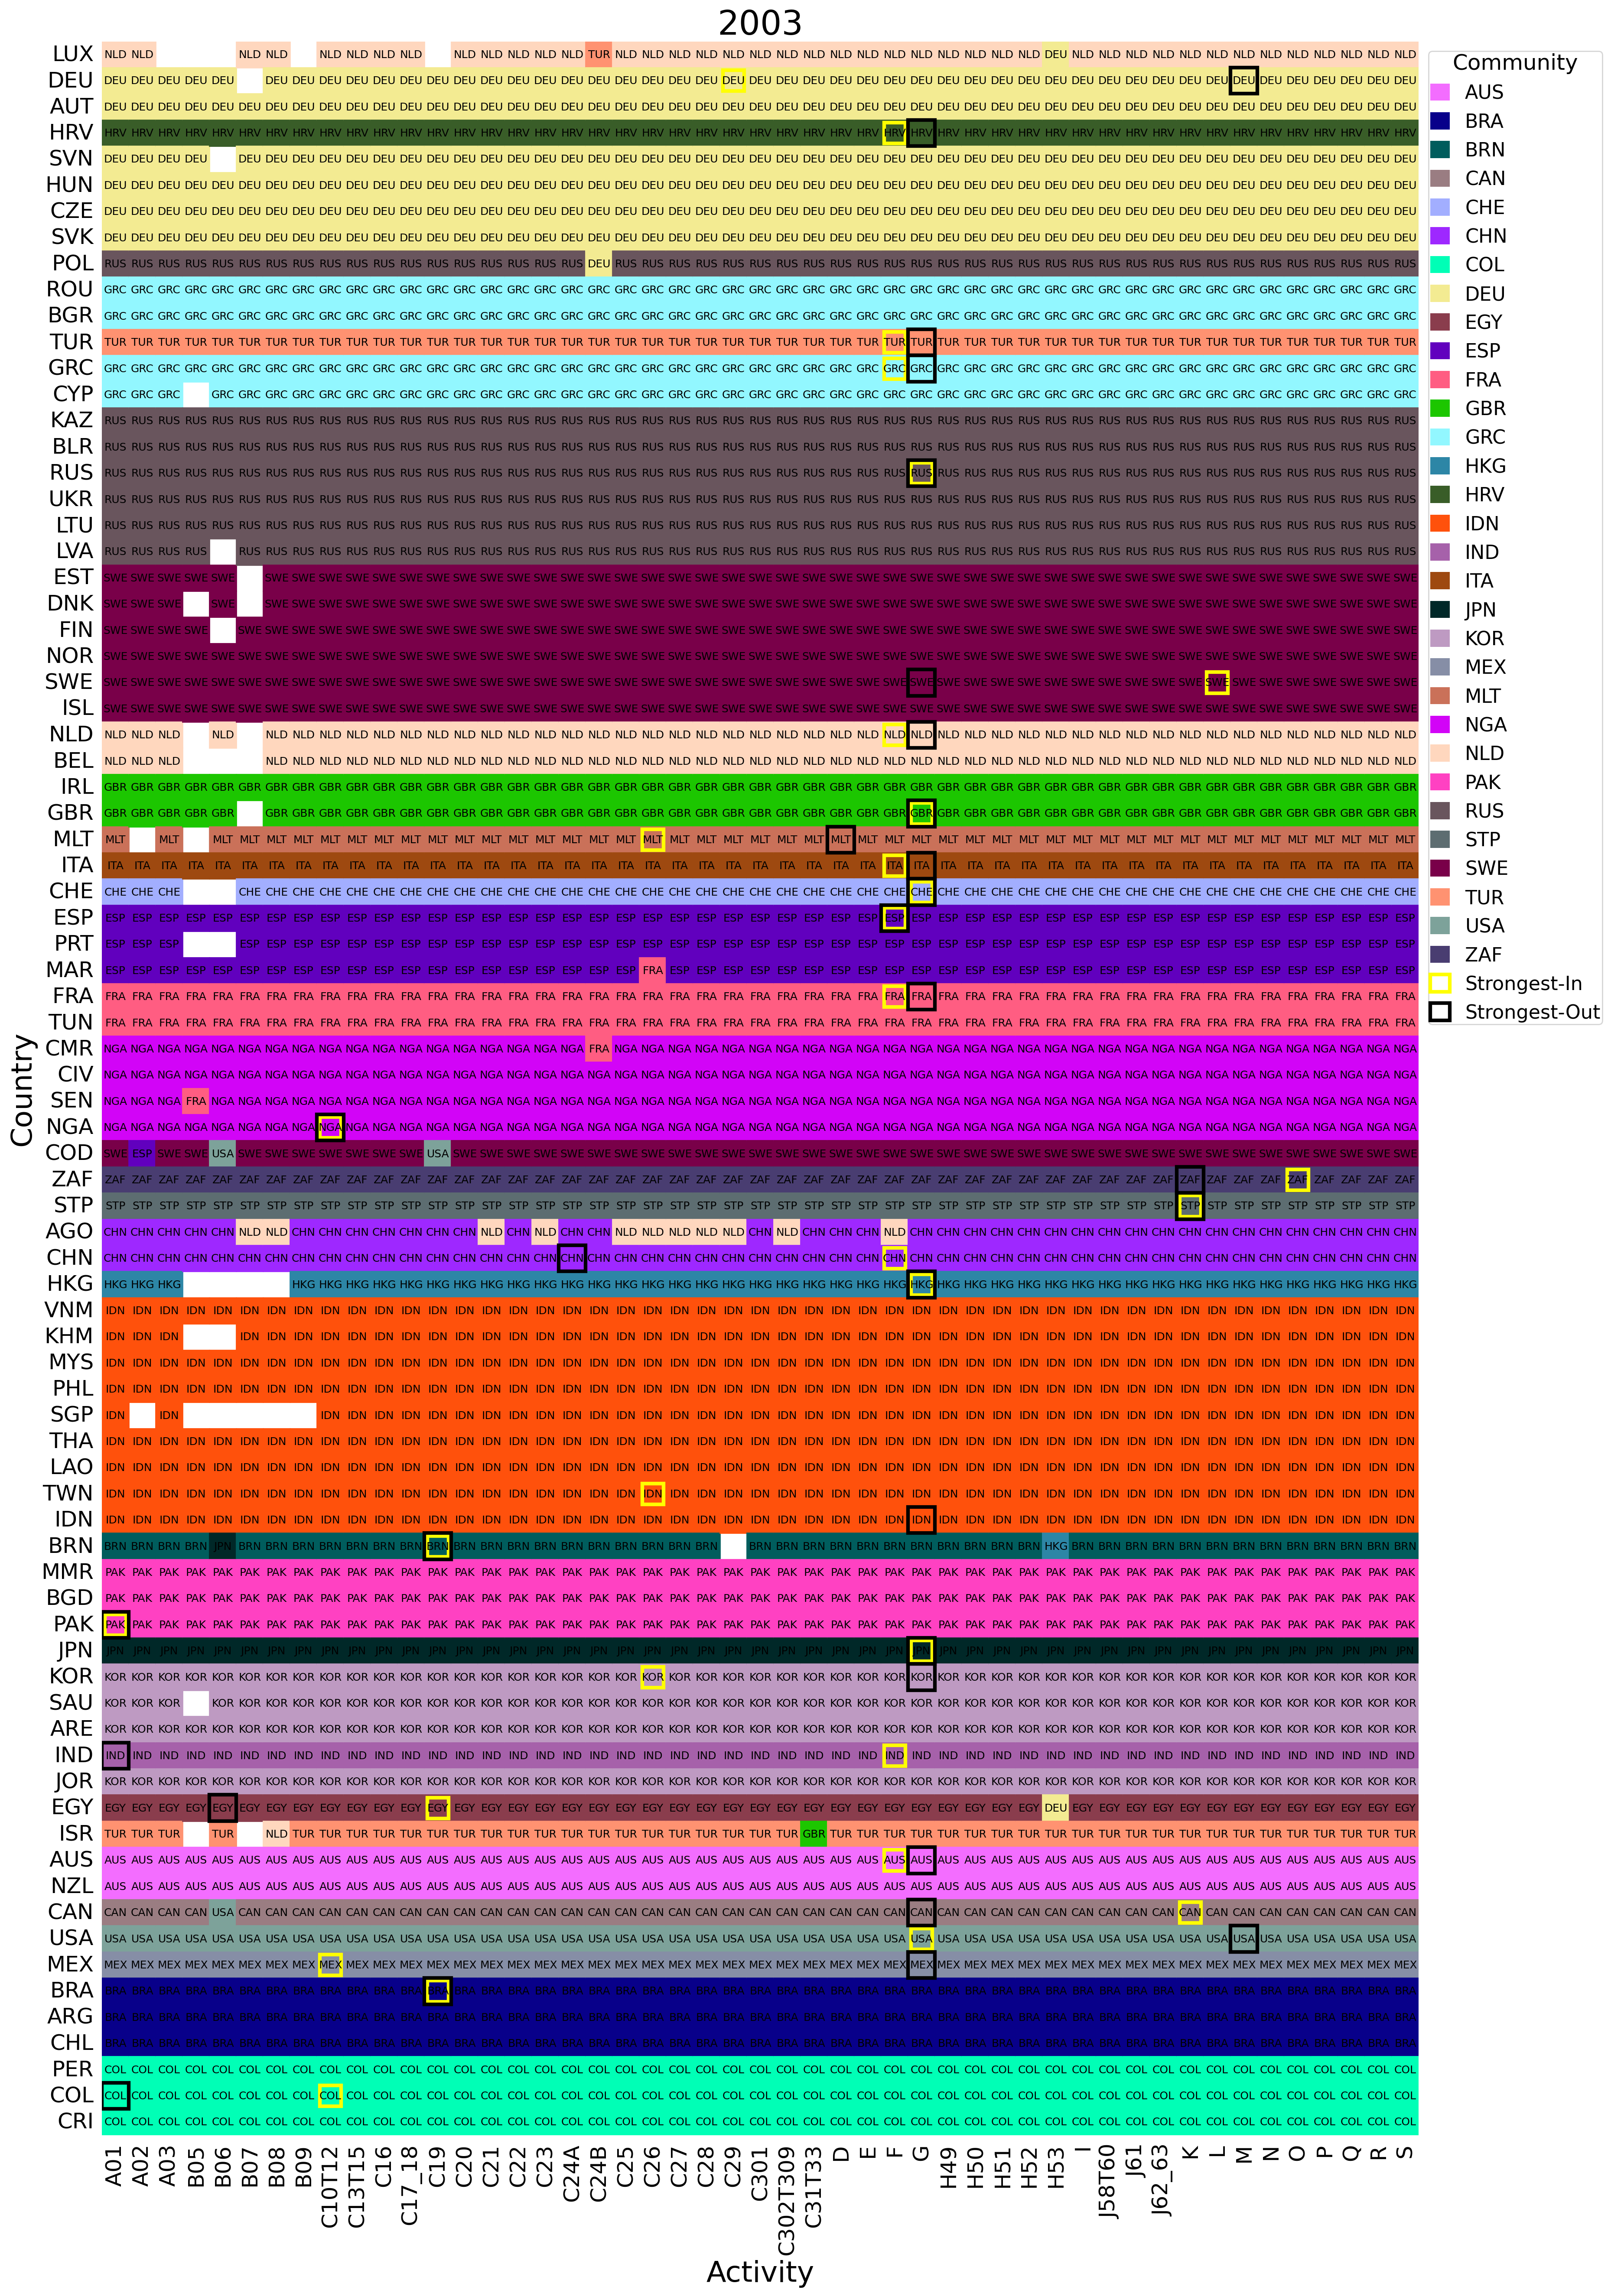
\includegraphics[width=\linewidth]{2003_communities.png}
	\caption{Resultados de la detección de comunidades en 2003.}
	\label{Fig_2003_comunidades}
\end{figure}

\begin{figure}[H]
	\centering
	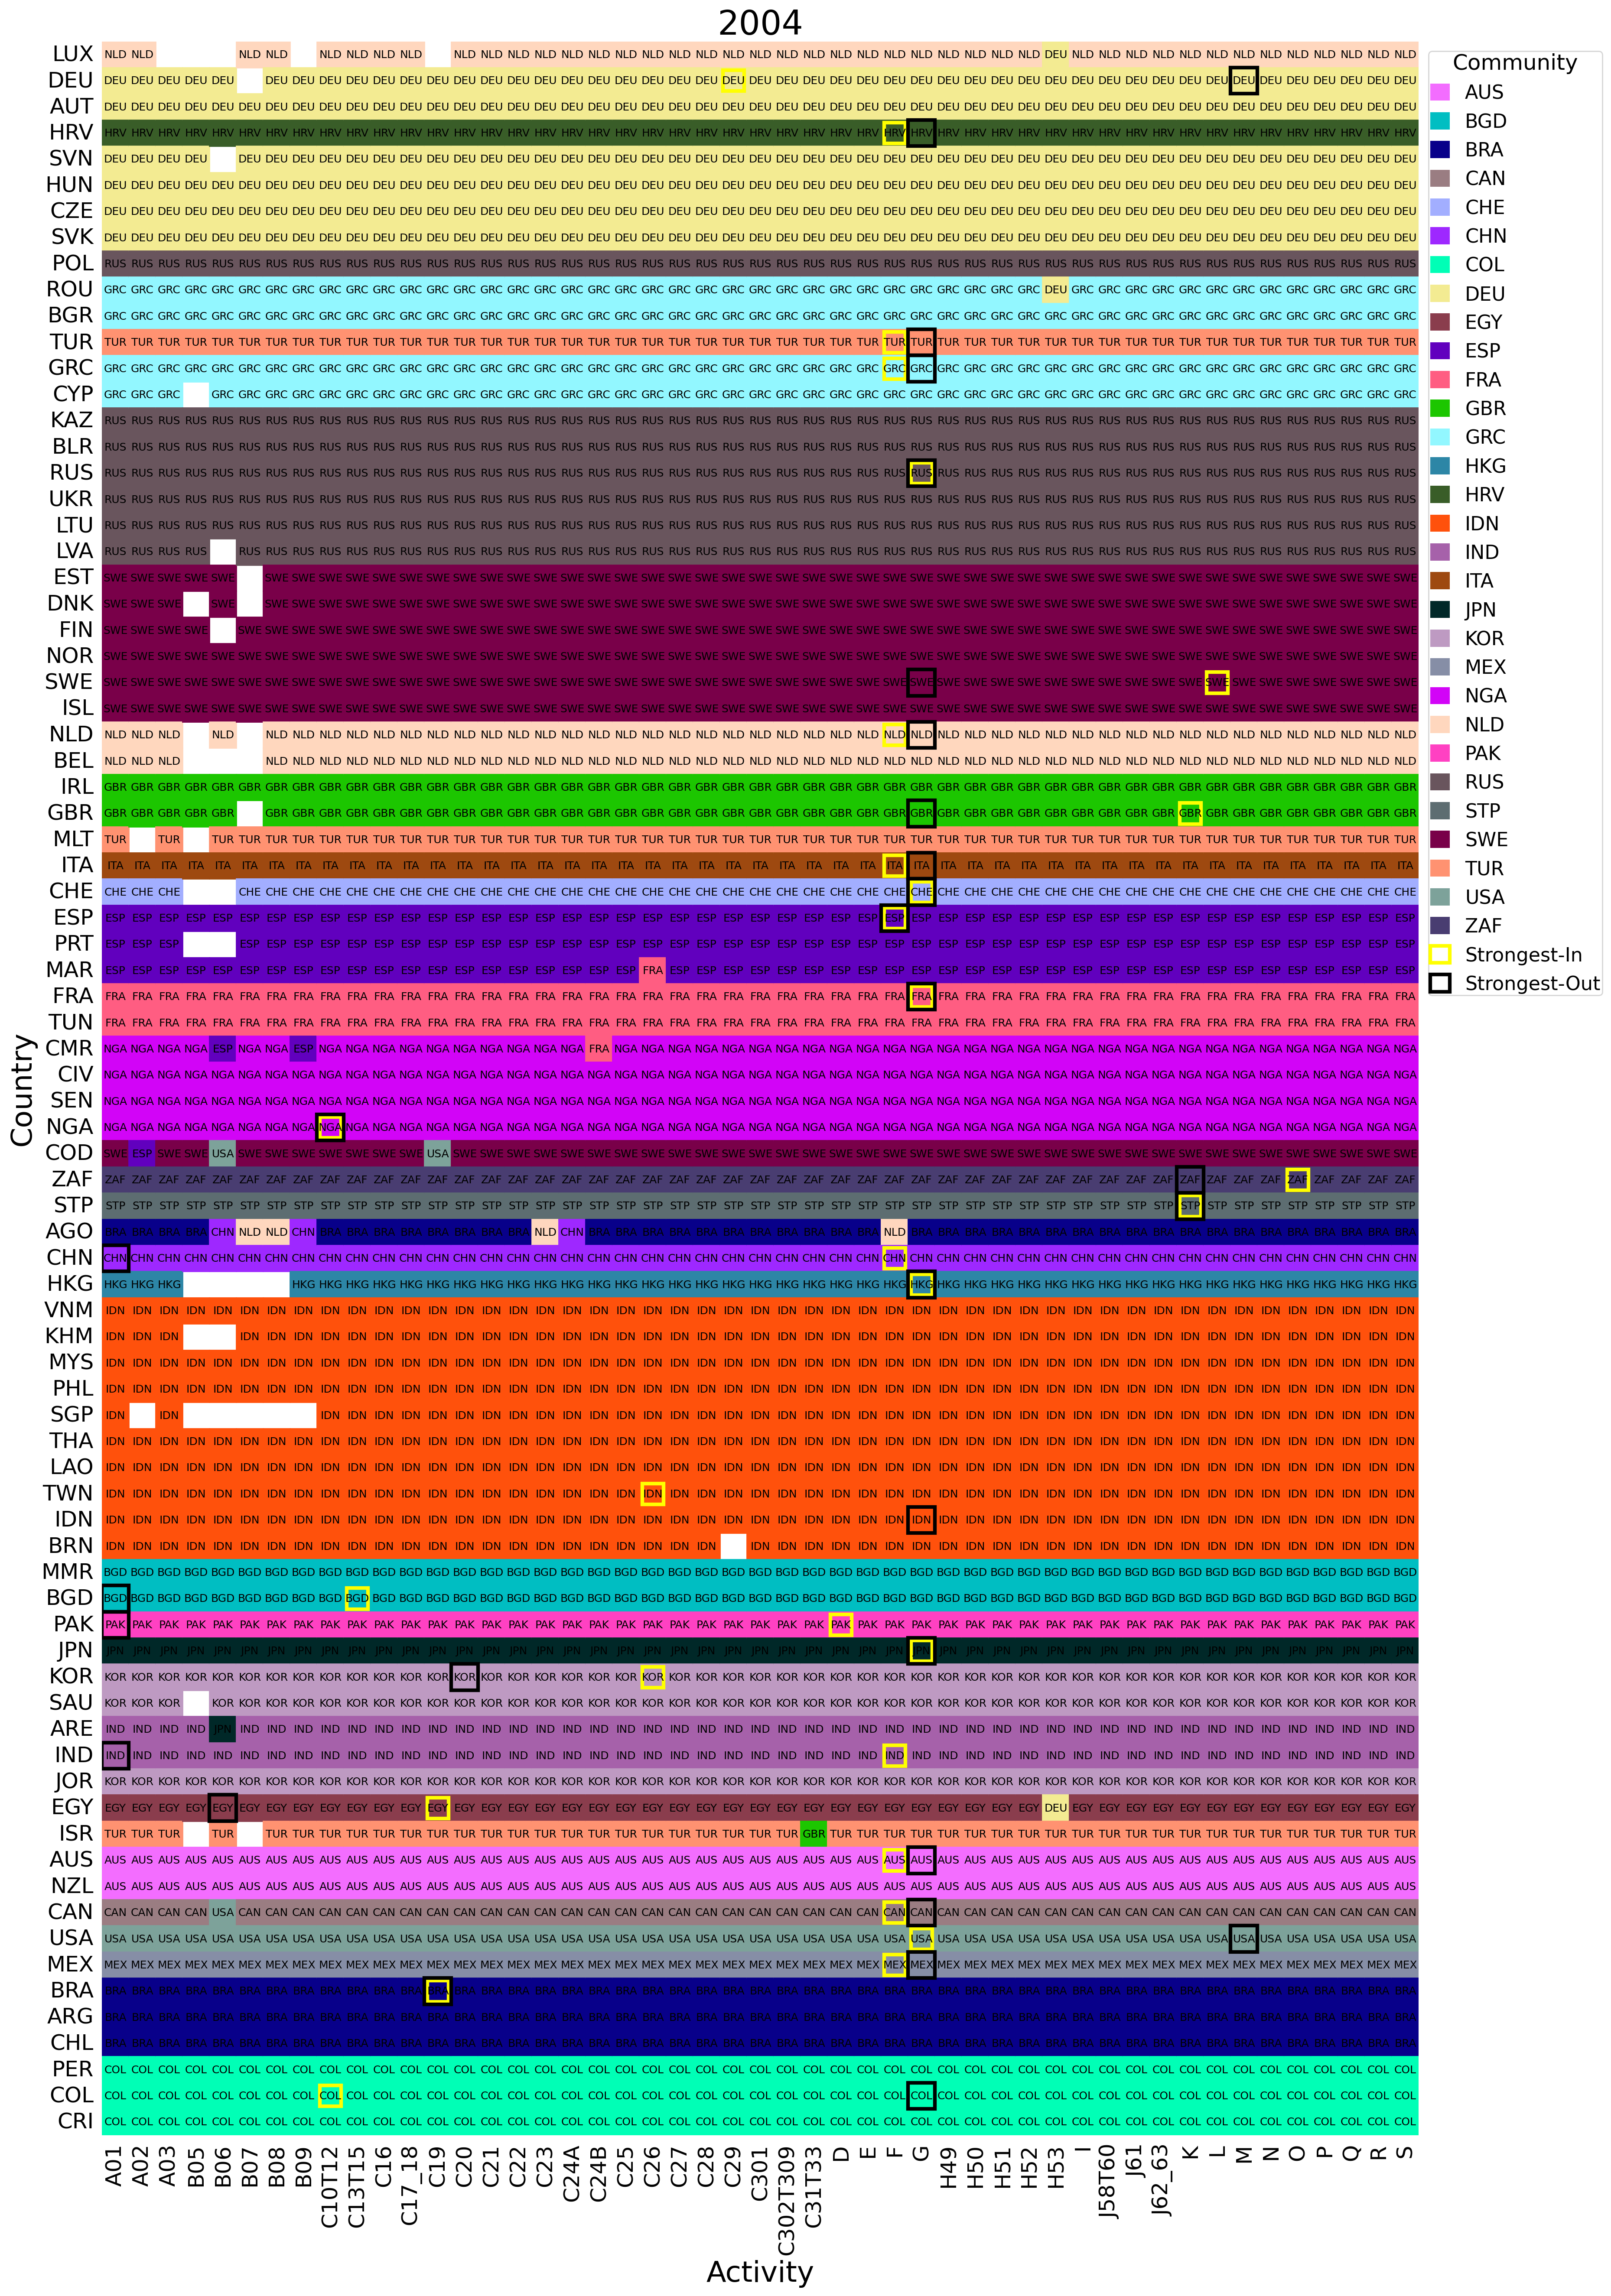
\includegraphics[width=\linewidth]{2004_communities.png}
	\caption{Resultados de la detección de comunidades en 2004.}
	\label{Fig_2004_comunidades}
\end{figure}

\begin{figure}[H]
	\centering
	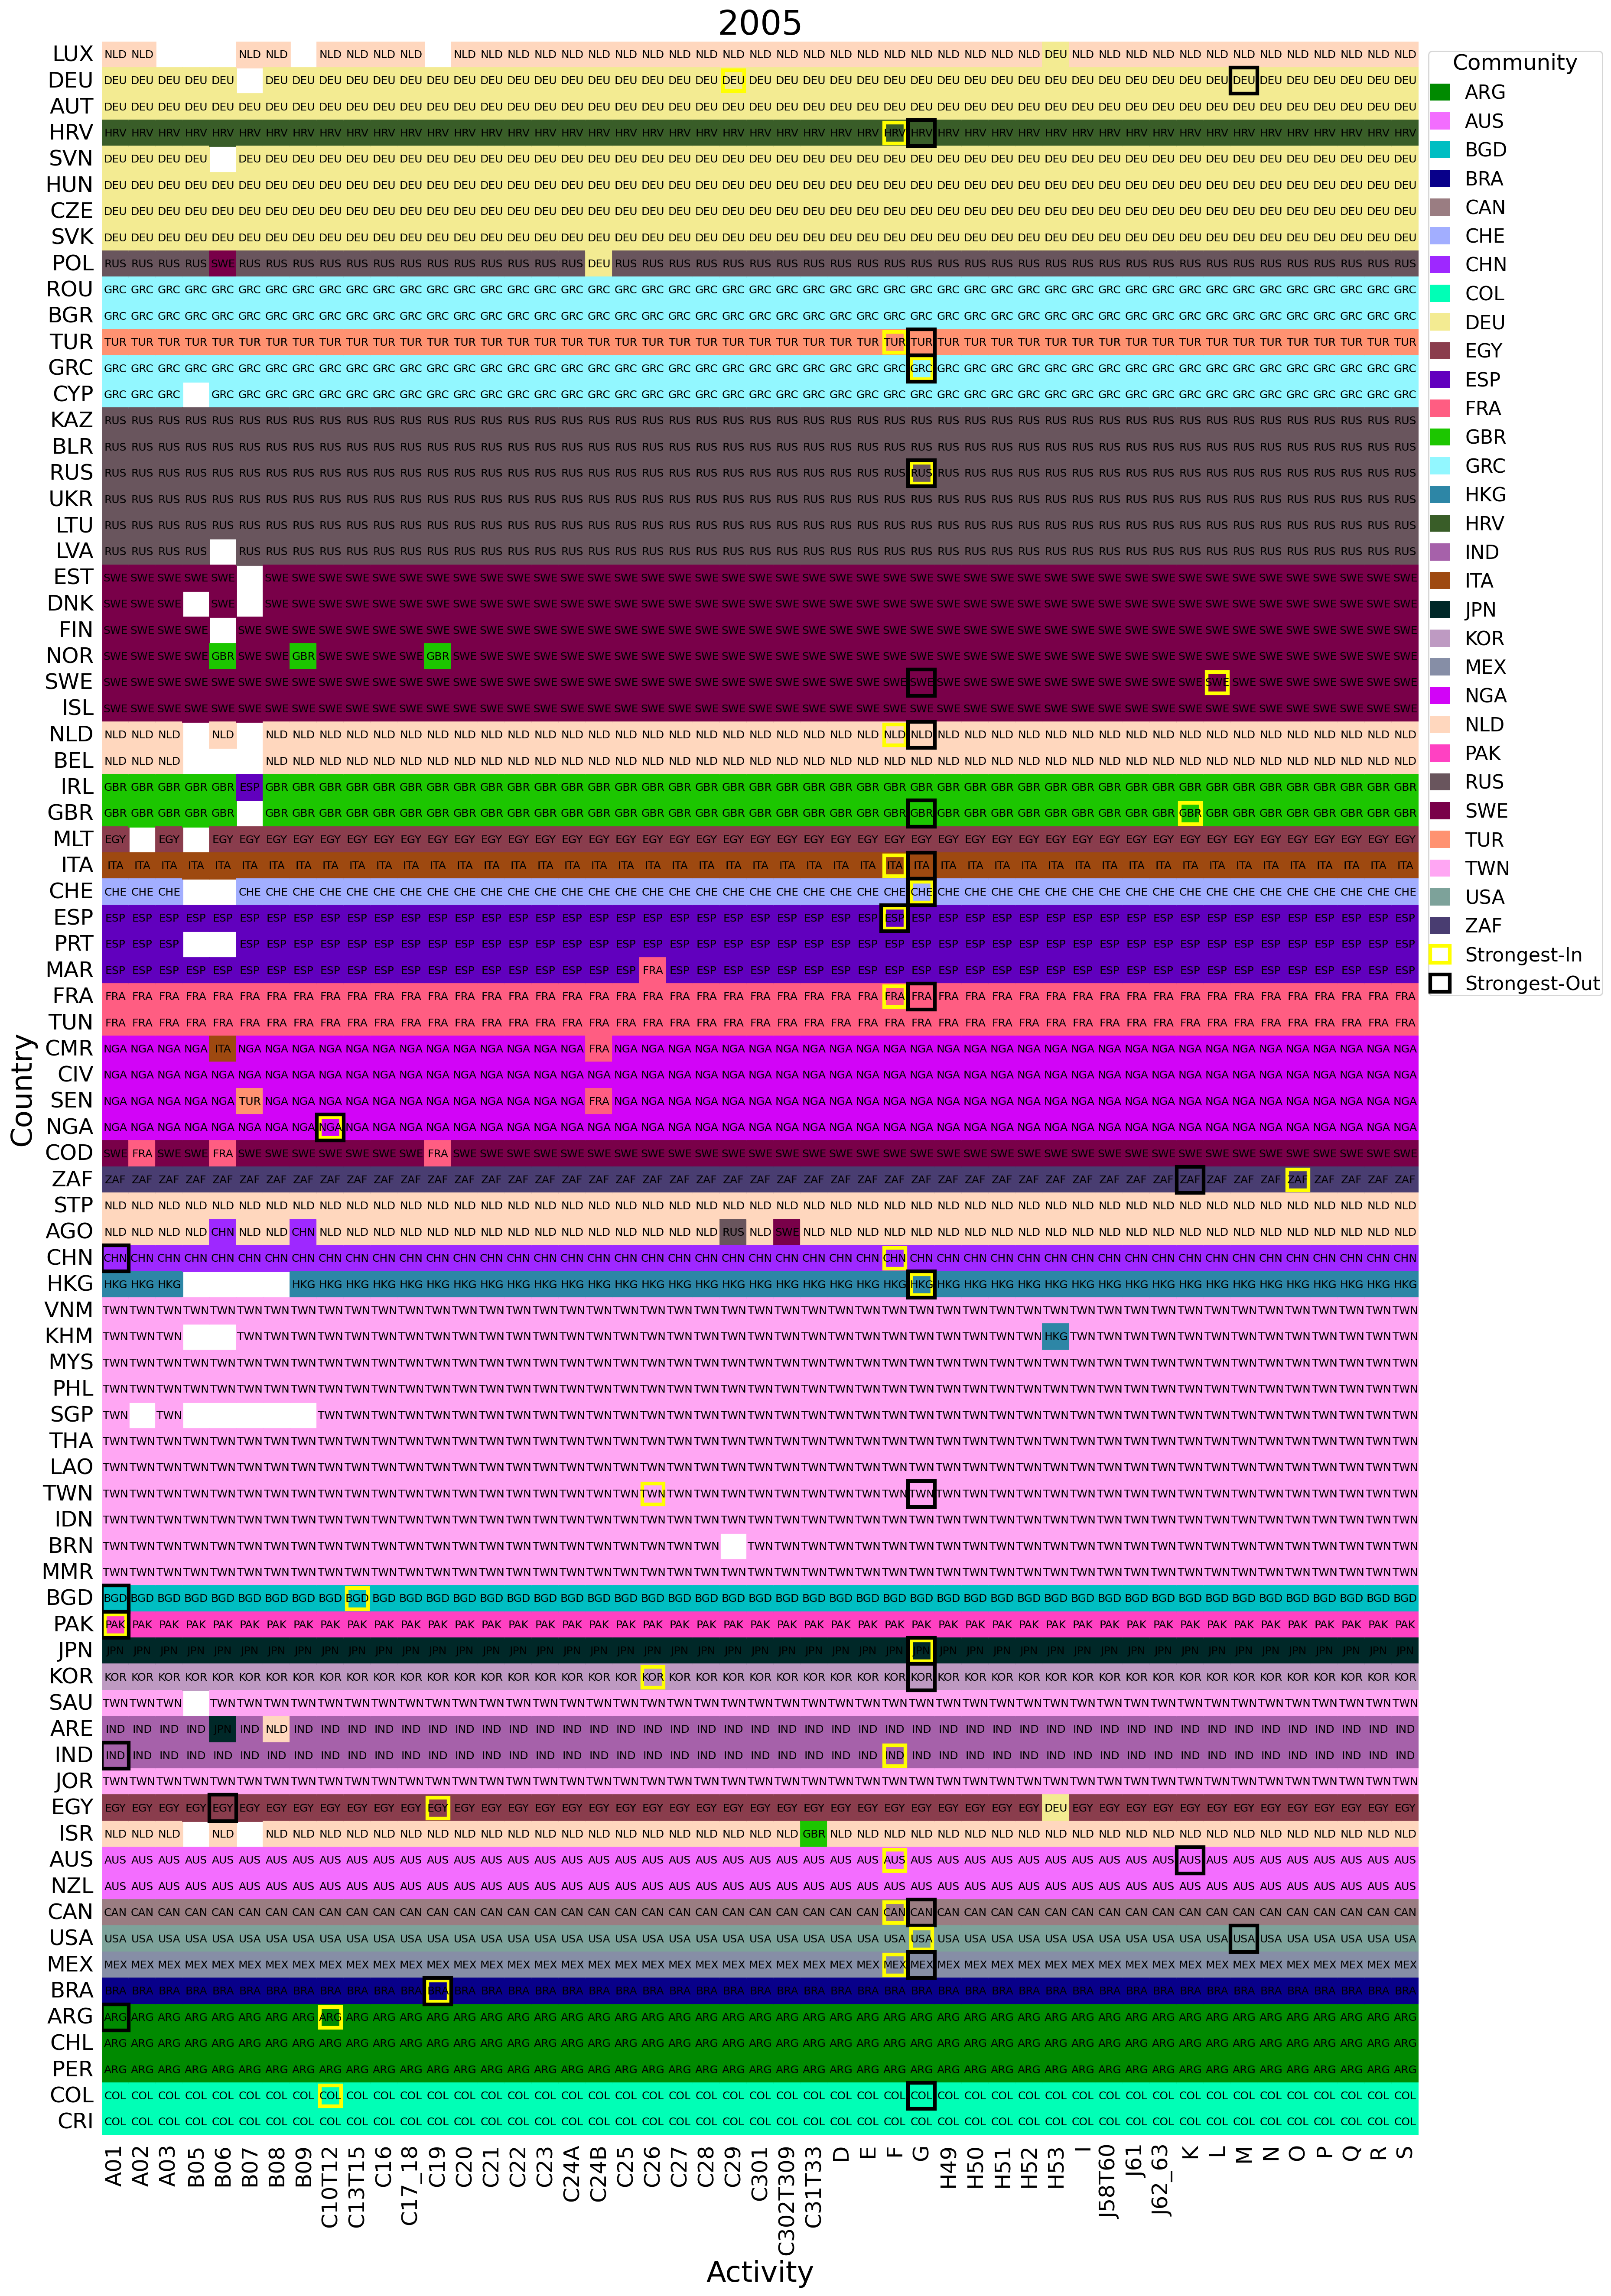
\includegraphics[width=\linewidth]{2005_communities.png}
	\caption{Resultados de la detección de comunidades en 2005.}
	\label{Fig_2005_comunidades}
\end{figure}

\begin{figure}[H]
	\centering
	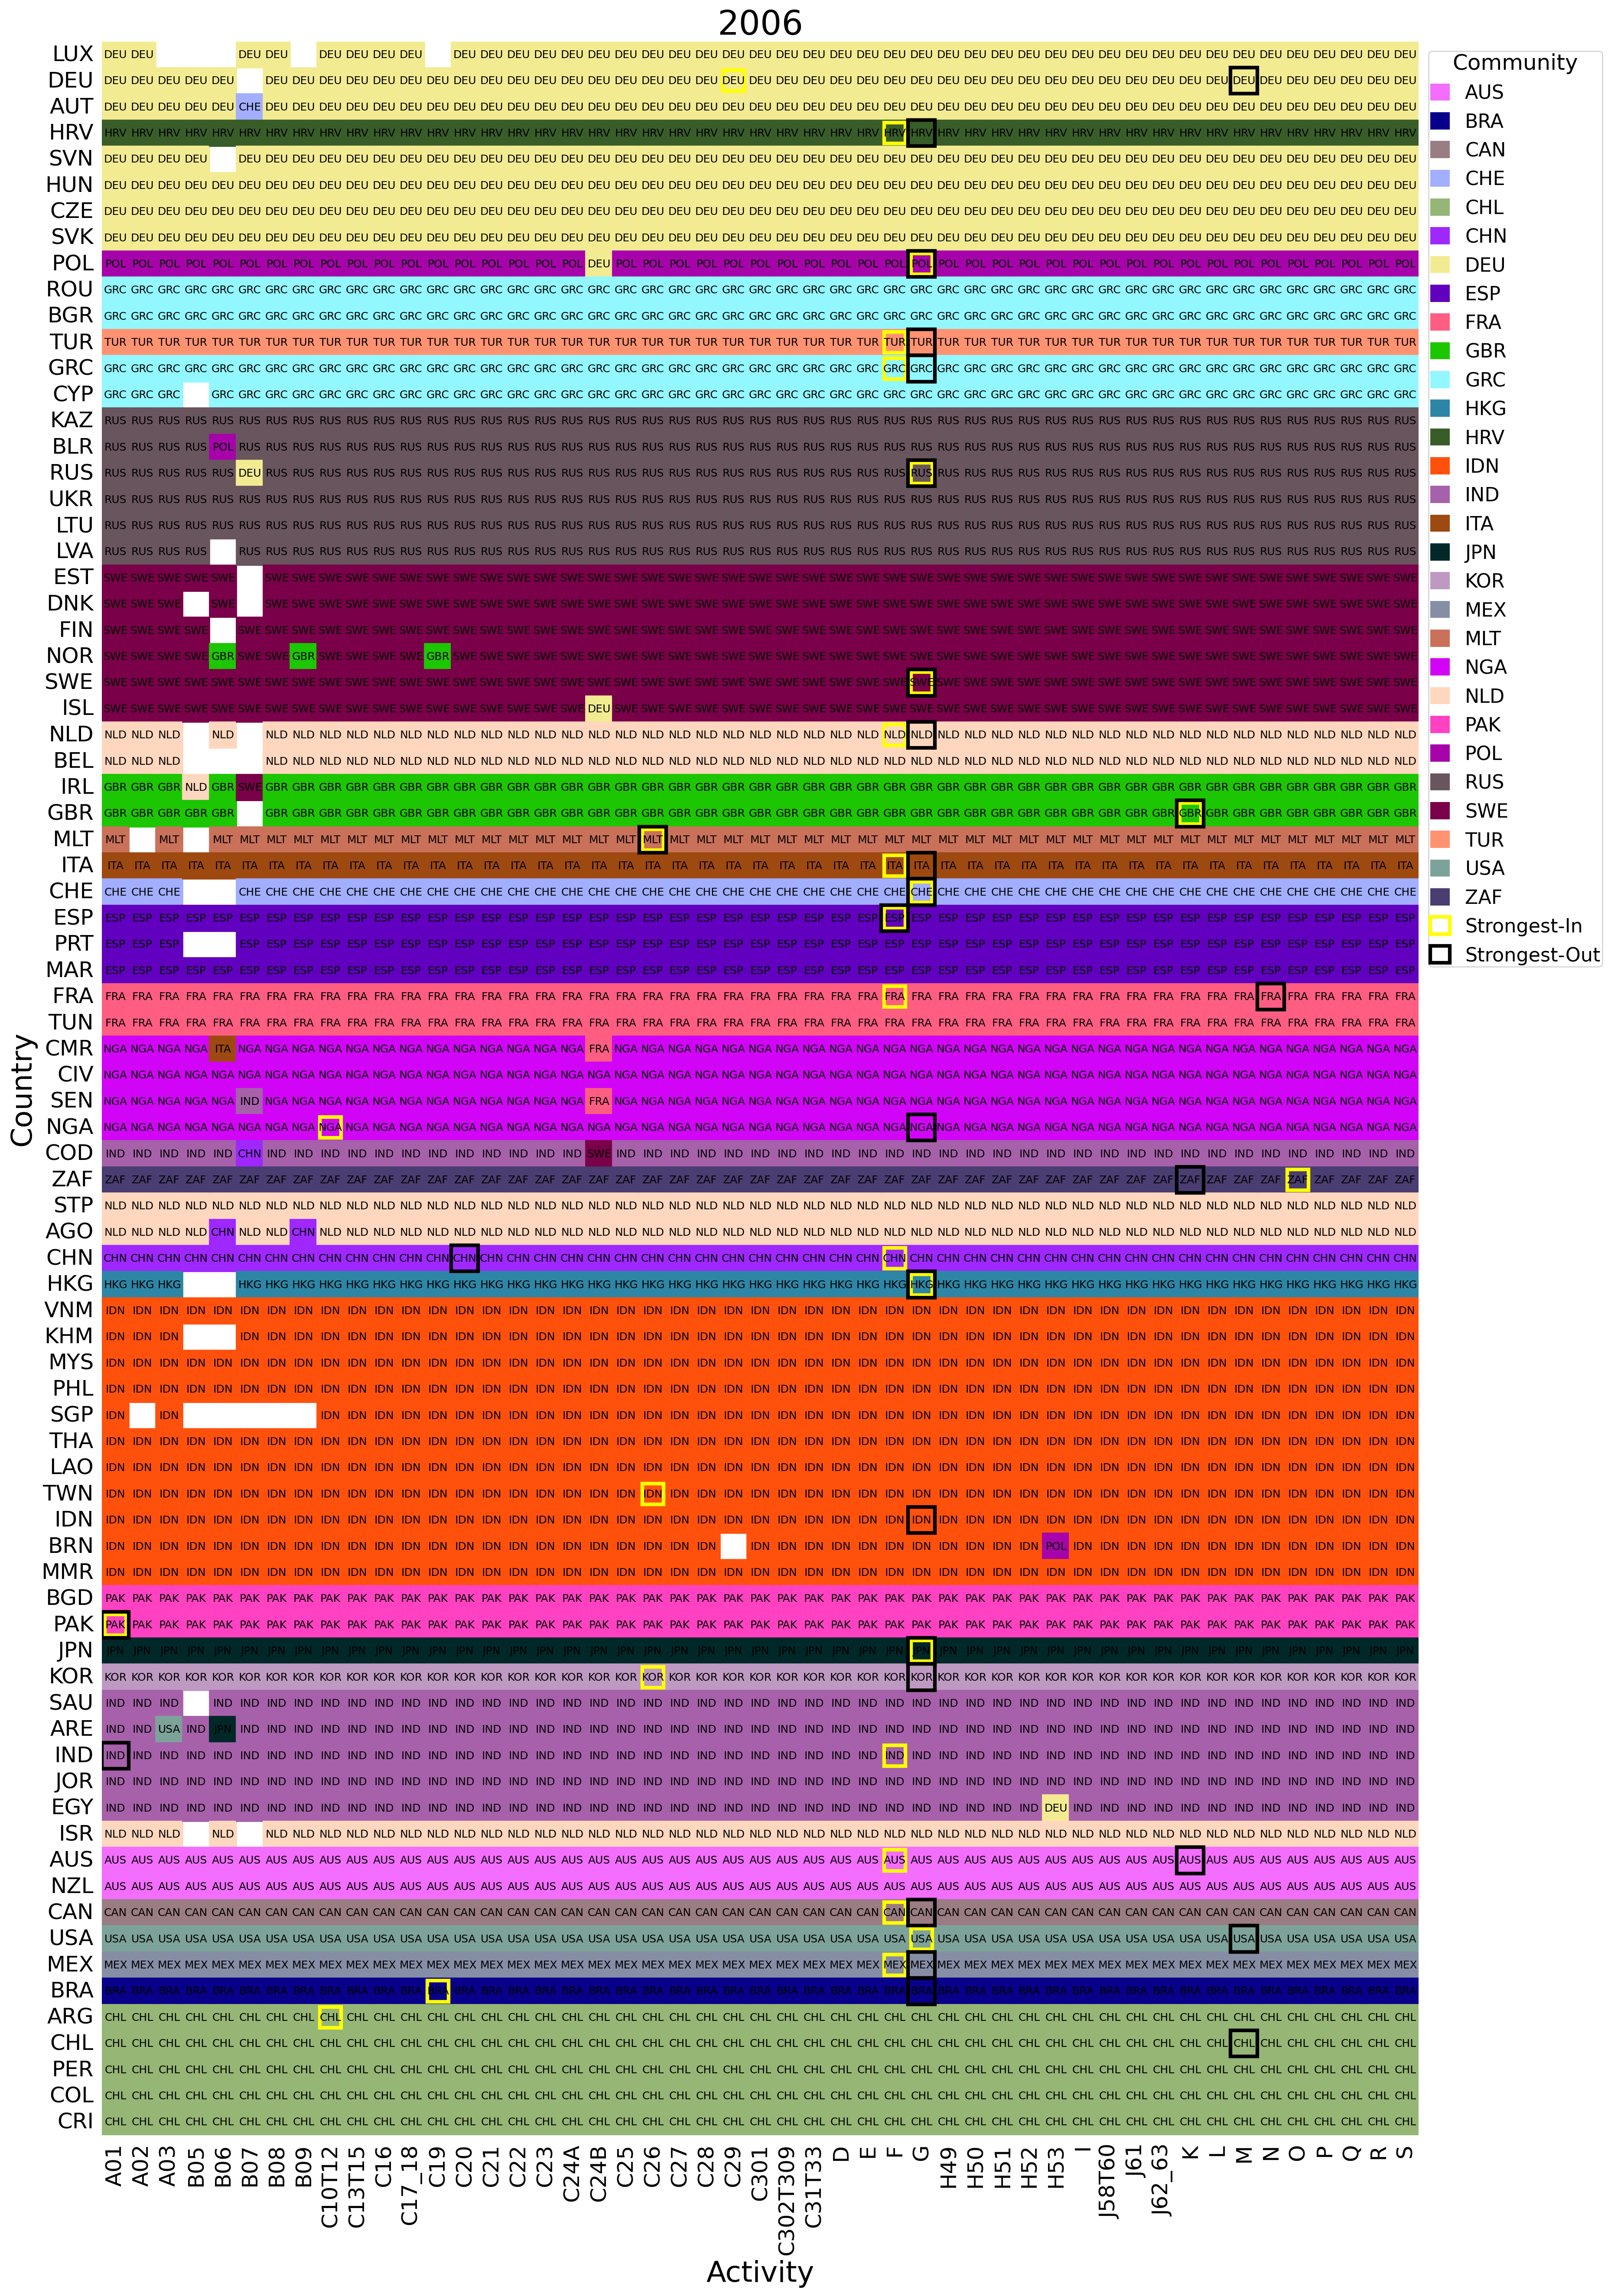
\includegraphics[width=\linewidth]{2006_communities.png}
	\caption{Resultados de la detección de comunidades en 2006.}
	\label{Fig_2006_comunidades}
\end{figure}

\begin{figure}[H]
	\centering
	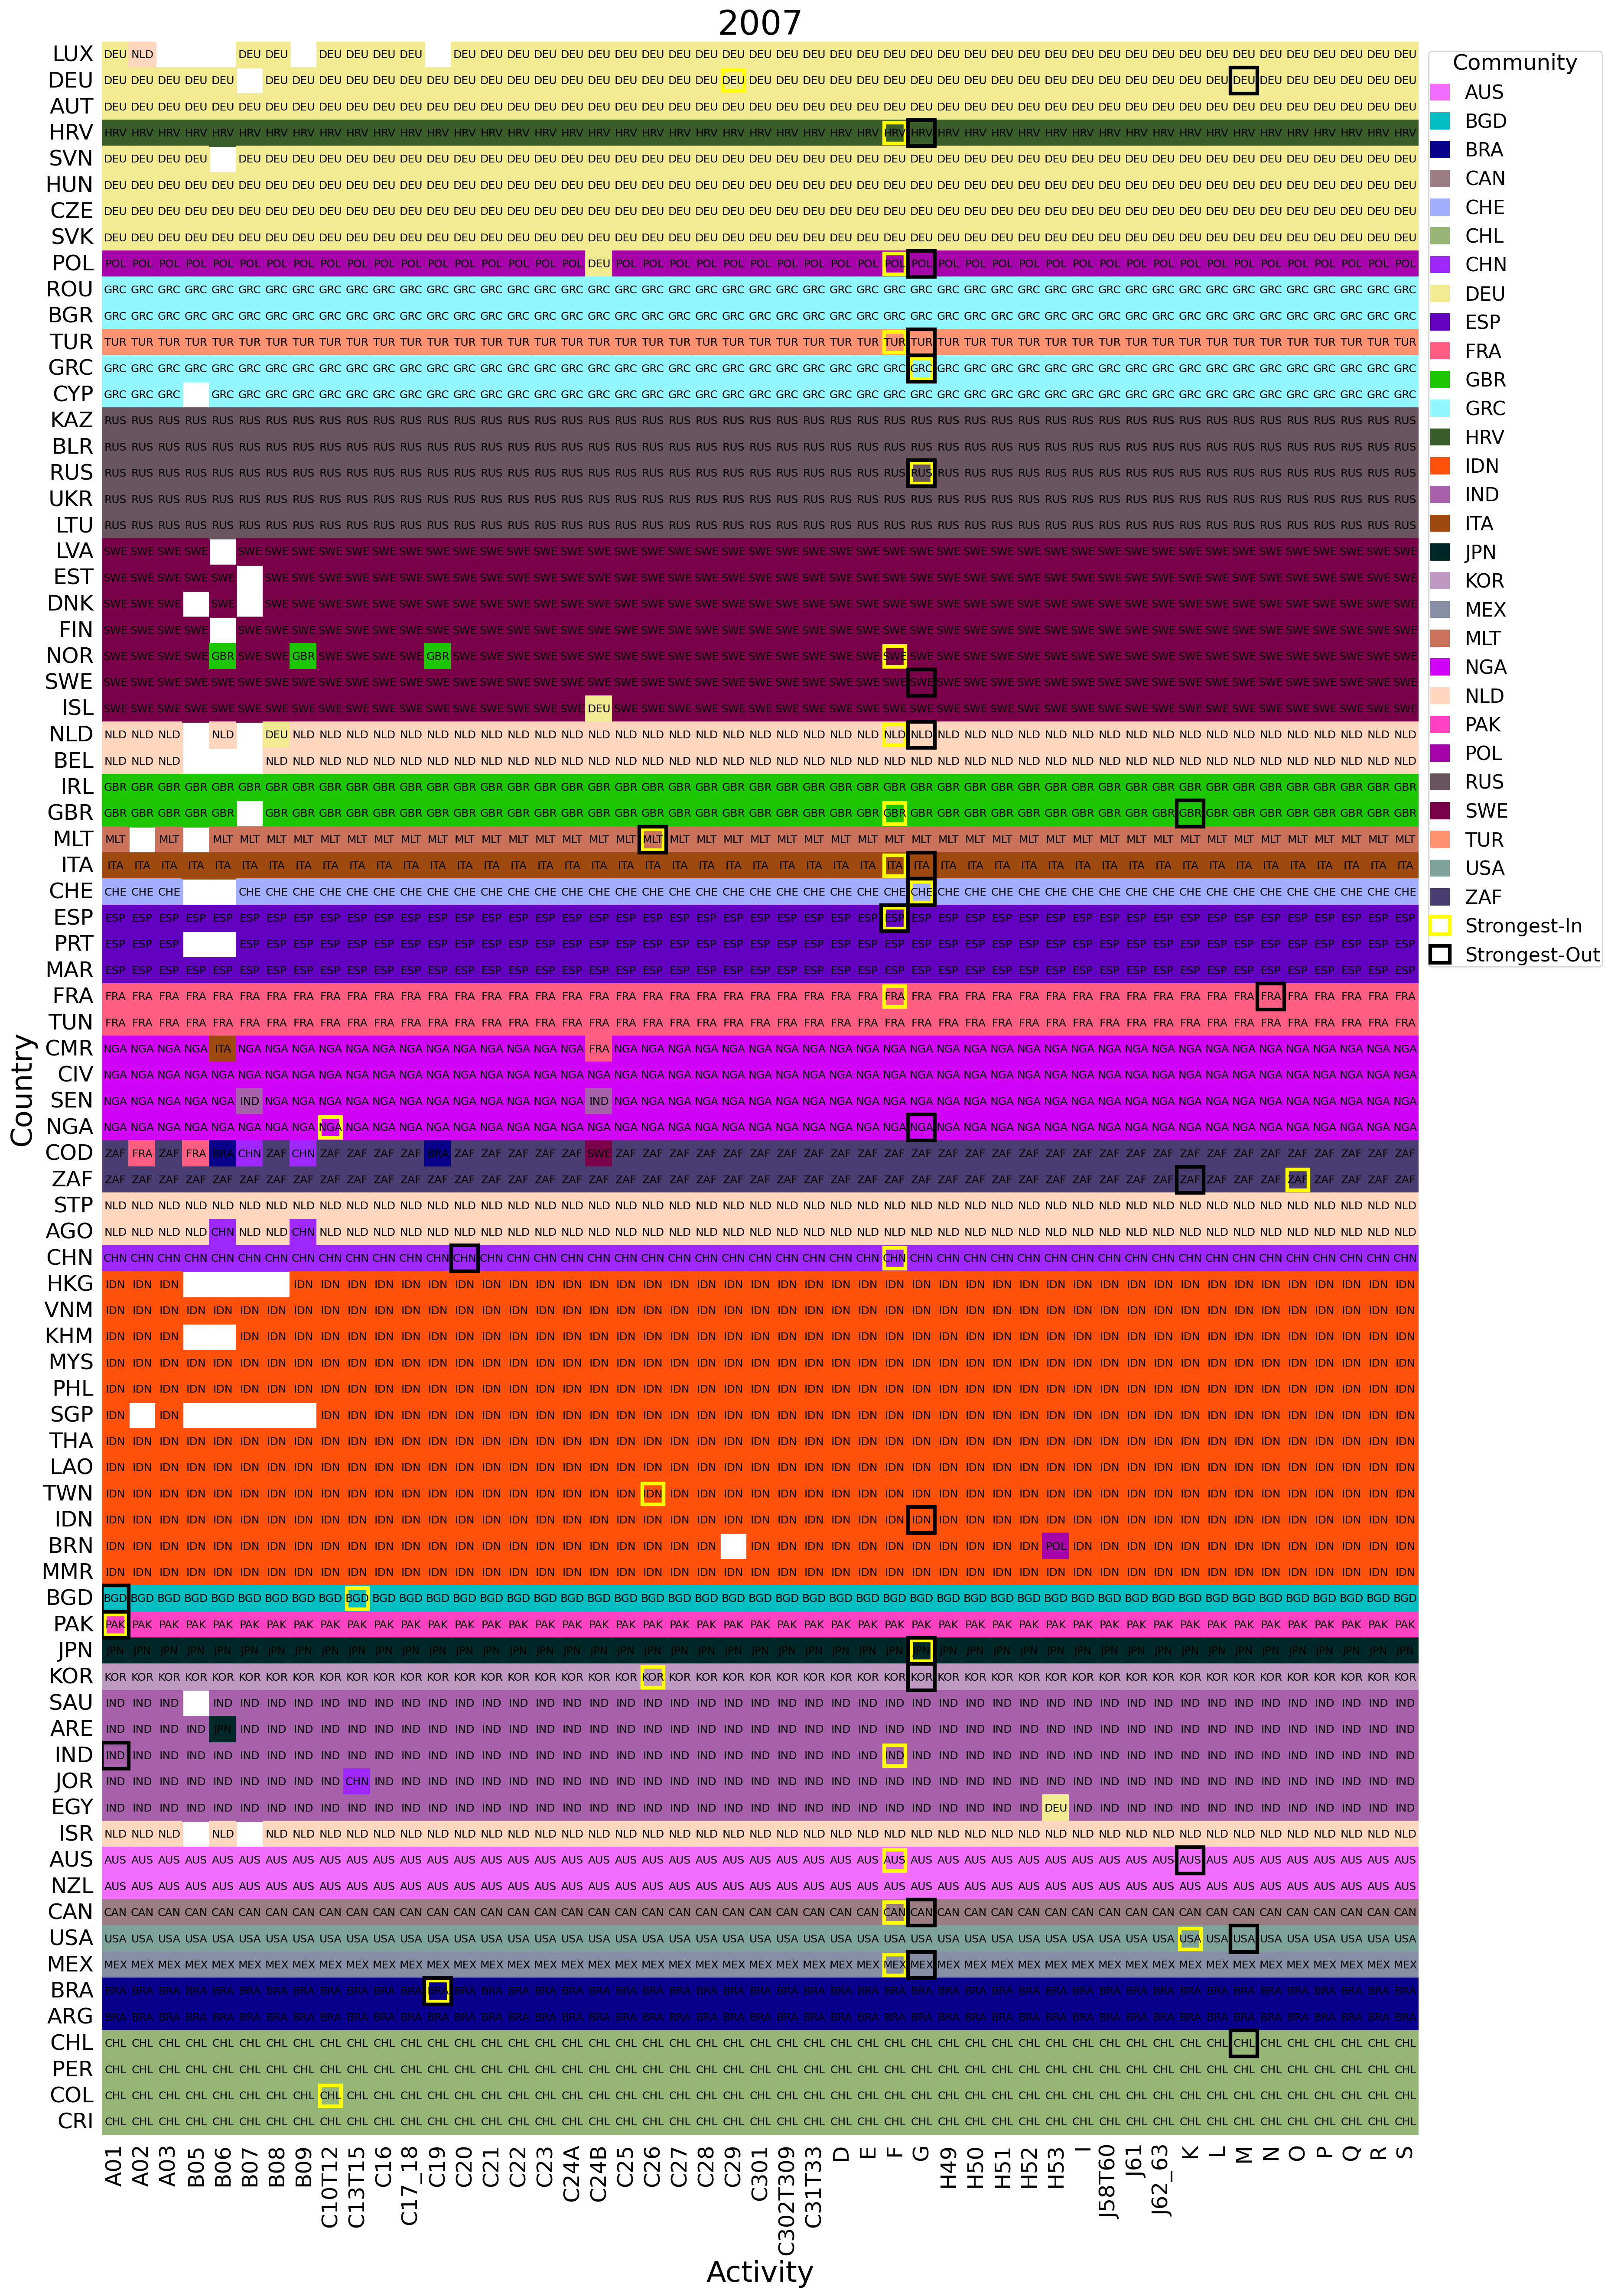
\includegraphics[width=\linewidth]{2007_communities.png}
	\caption{Resultados de la detección de comunidades en 2007.}
	\label{Fig_2007_comunidades}
\end{figure}

\begin{figure}[H]
	\centering
	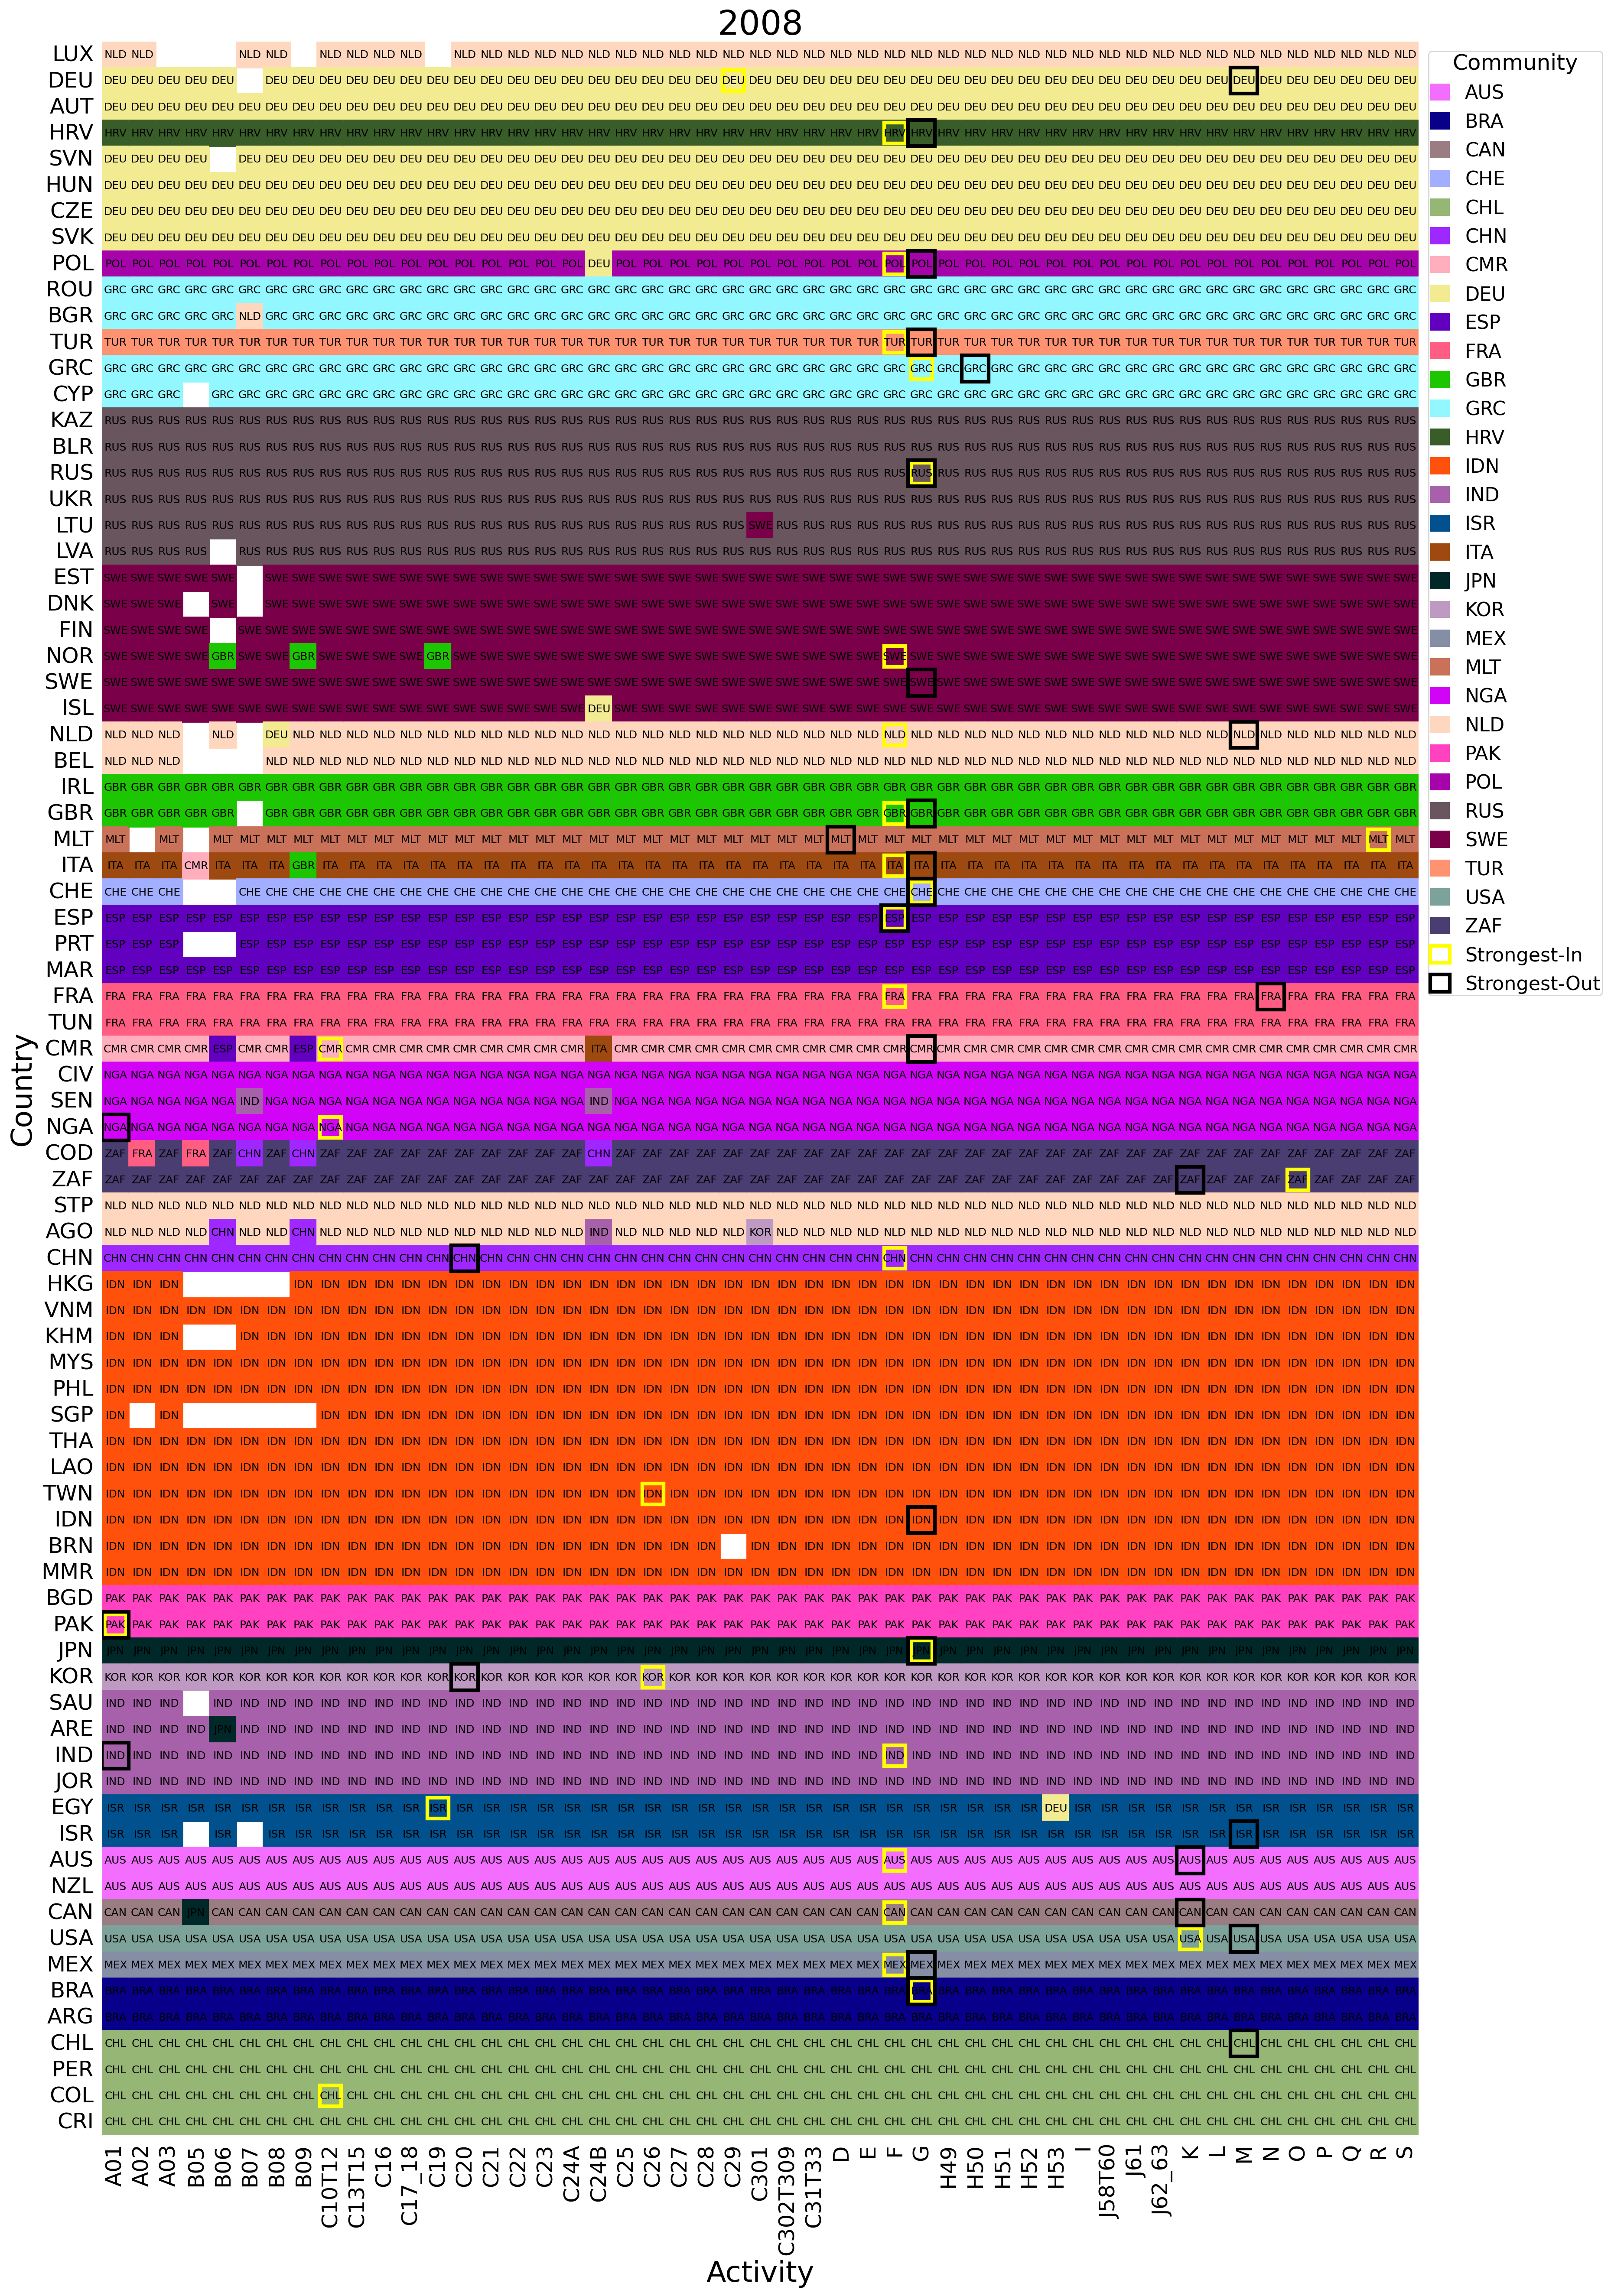
\includegraphics[width=\linewidth]{2008_communities.png}
	\caption{Resultados de la detección de comunidades en 2008.}
	\label{Fig_2008_comunidades}
\end{figure}

\begin{figure}[H]
	\centering
	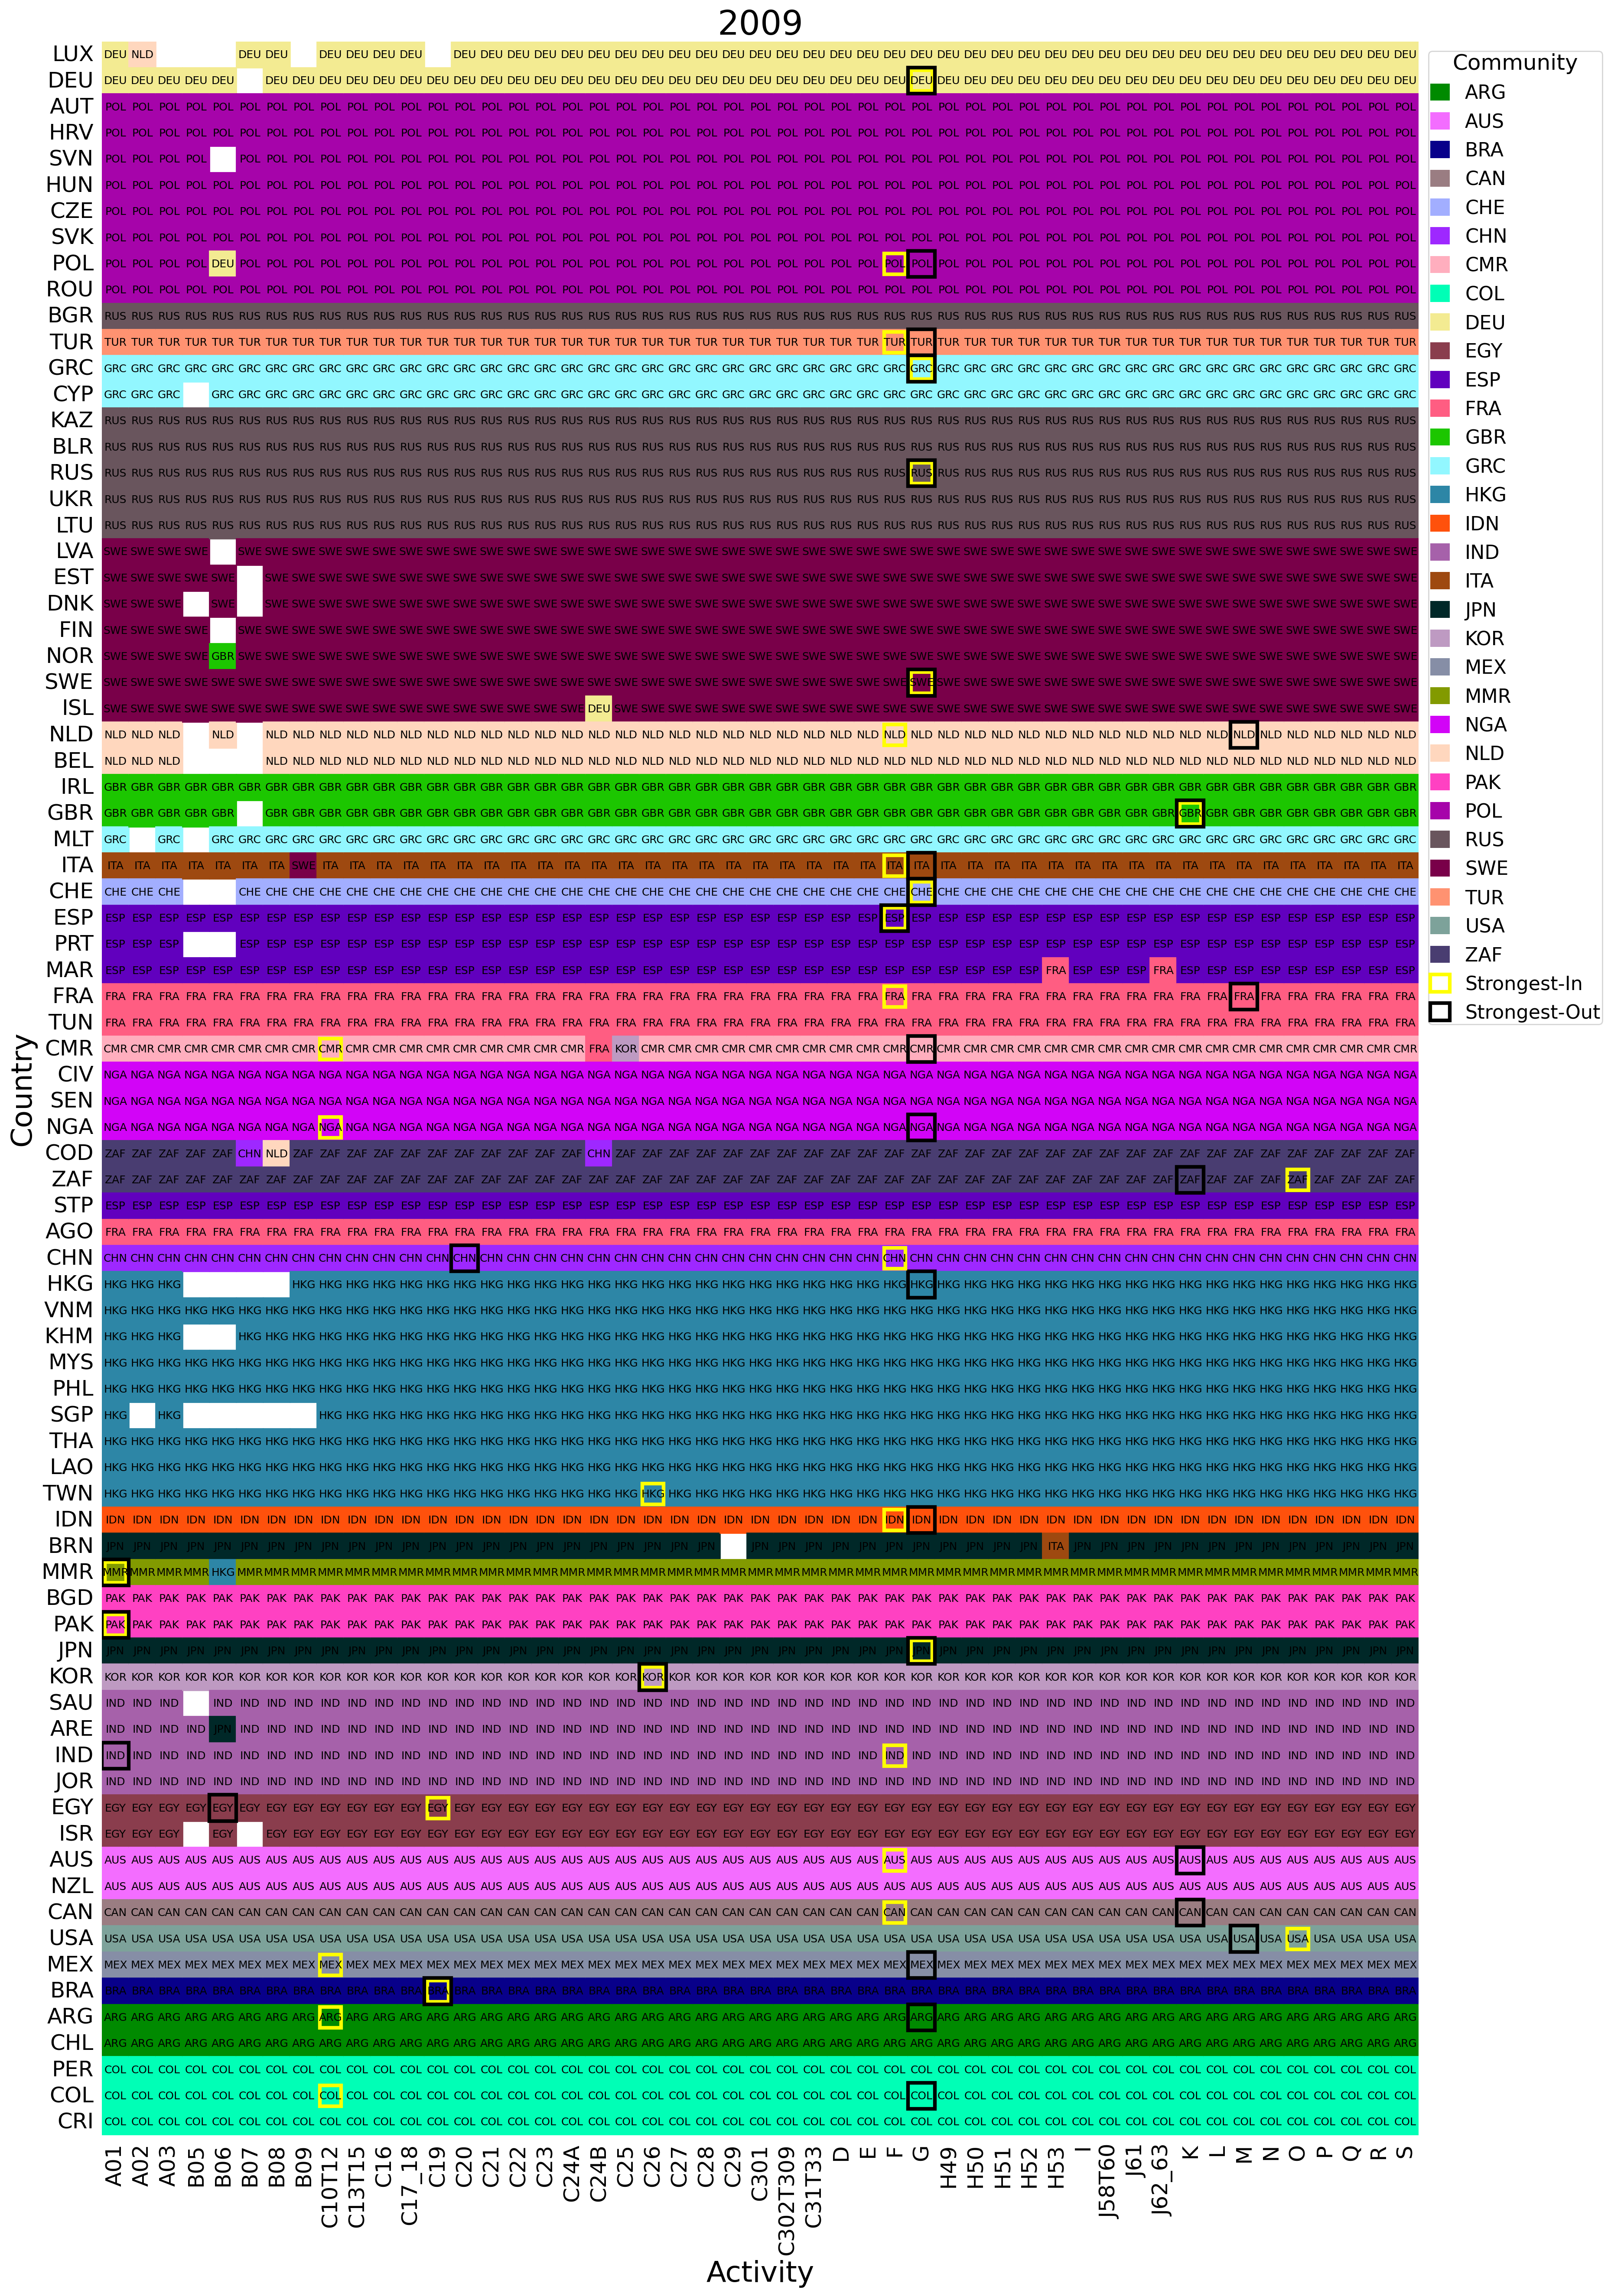
\includegraphics[width=\linewidth]{2009_communities.png}
	\caption{Resultados de la detección de comunidades en 2009.}
	\label{Fig_2009_comunidades}
\end{figure}

\begin{figure}[H]
	\centering
	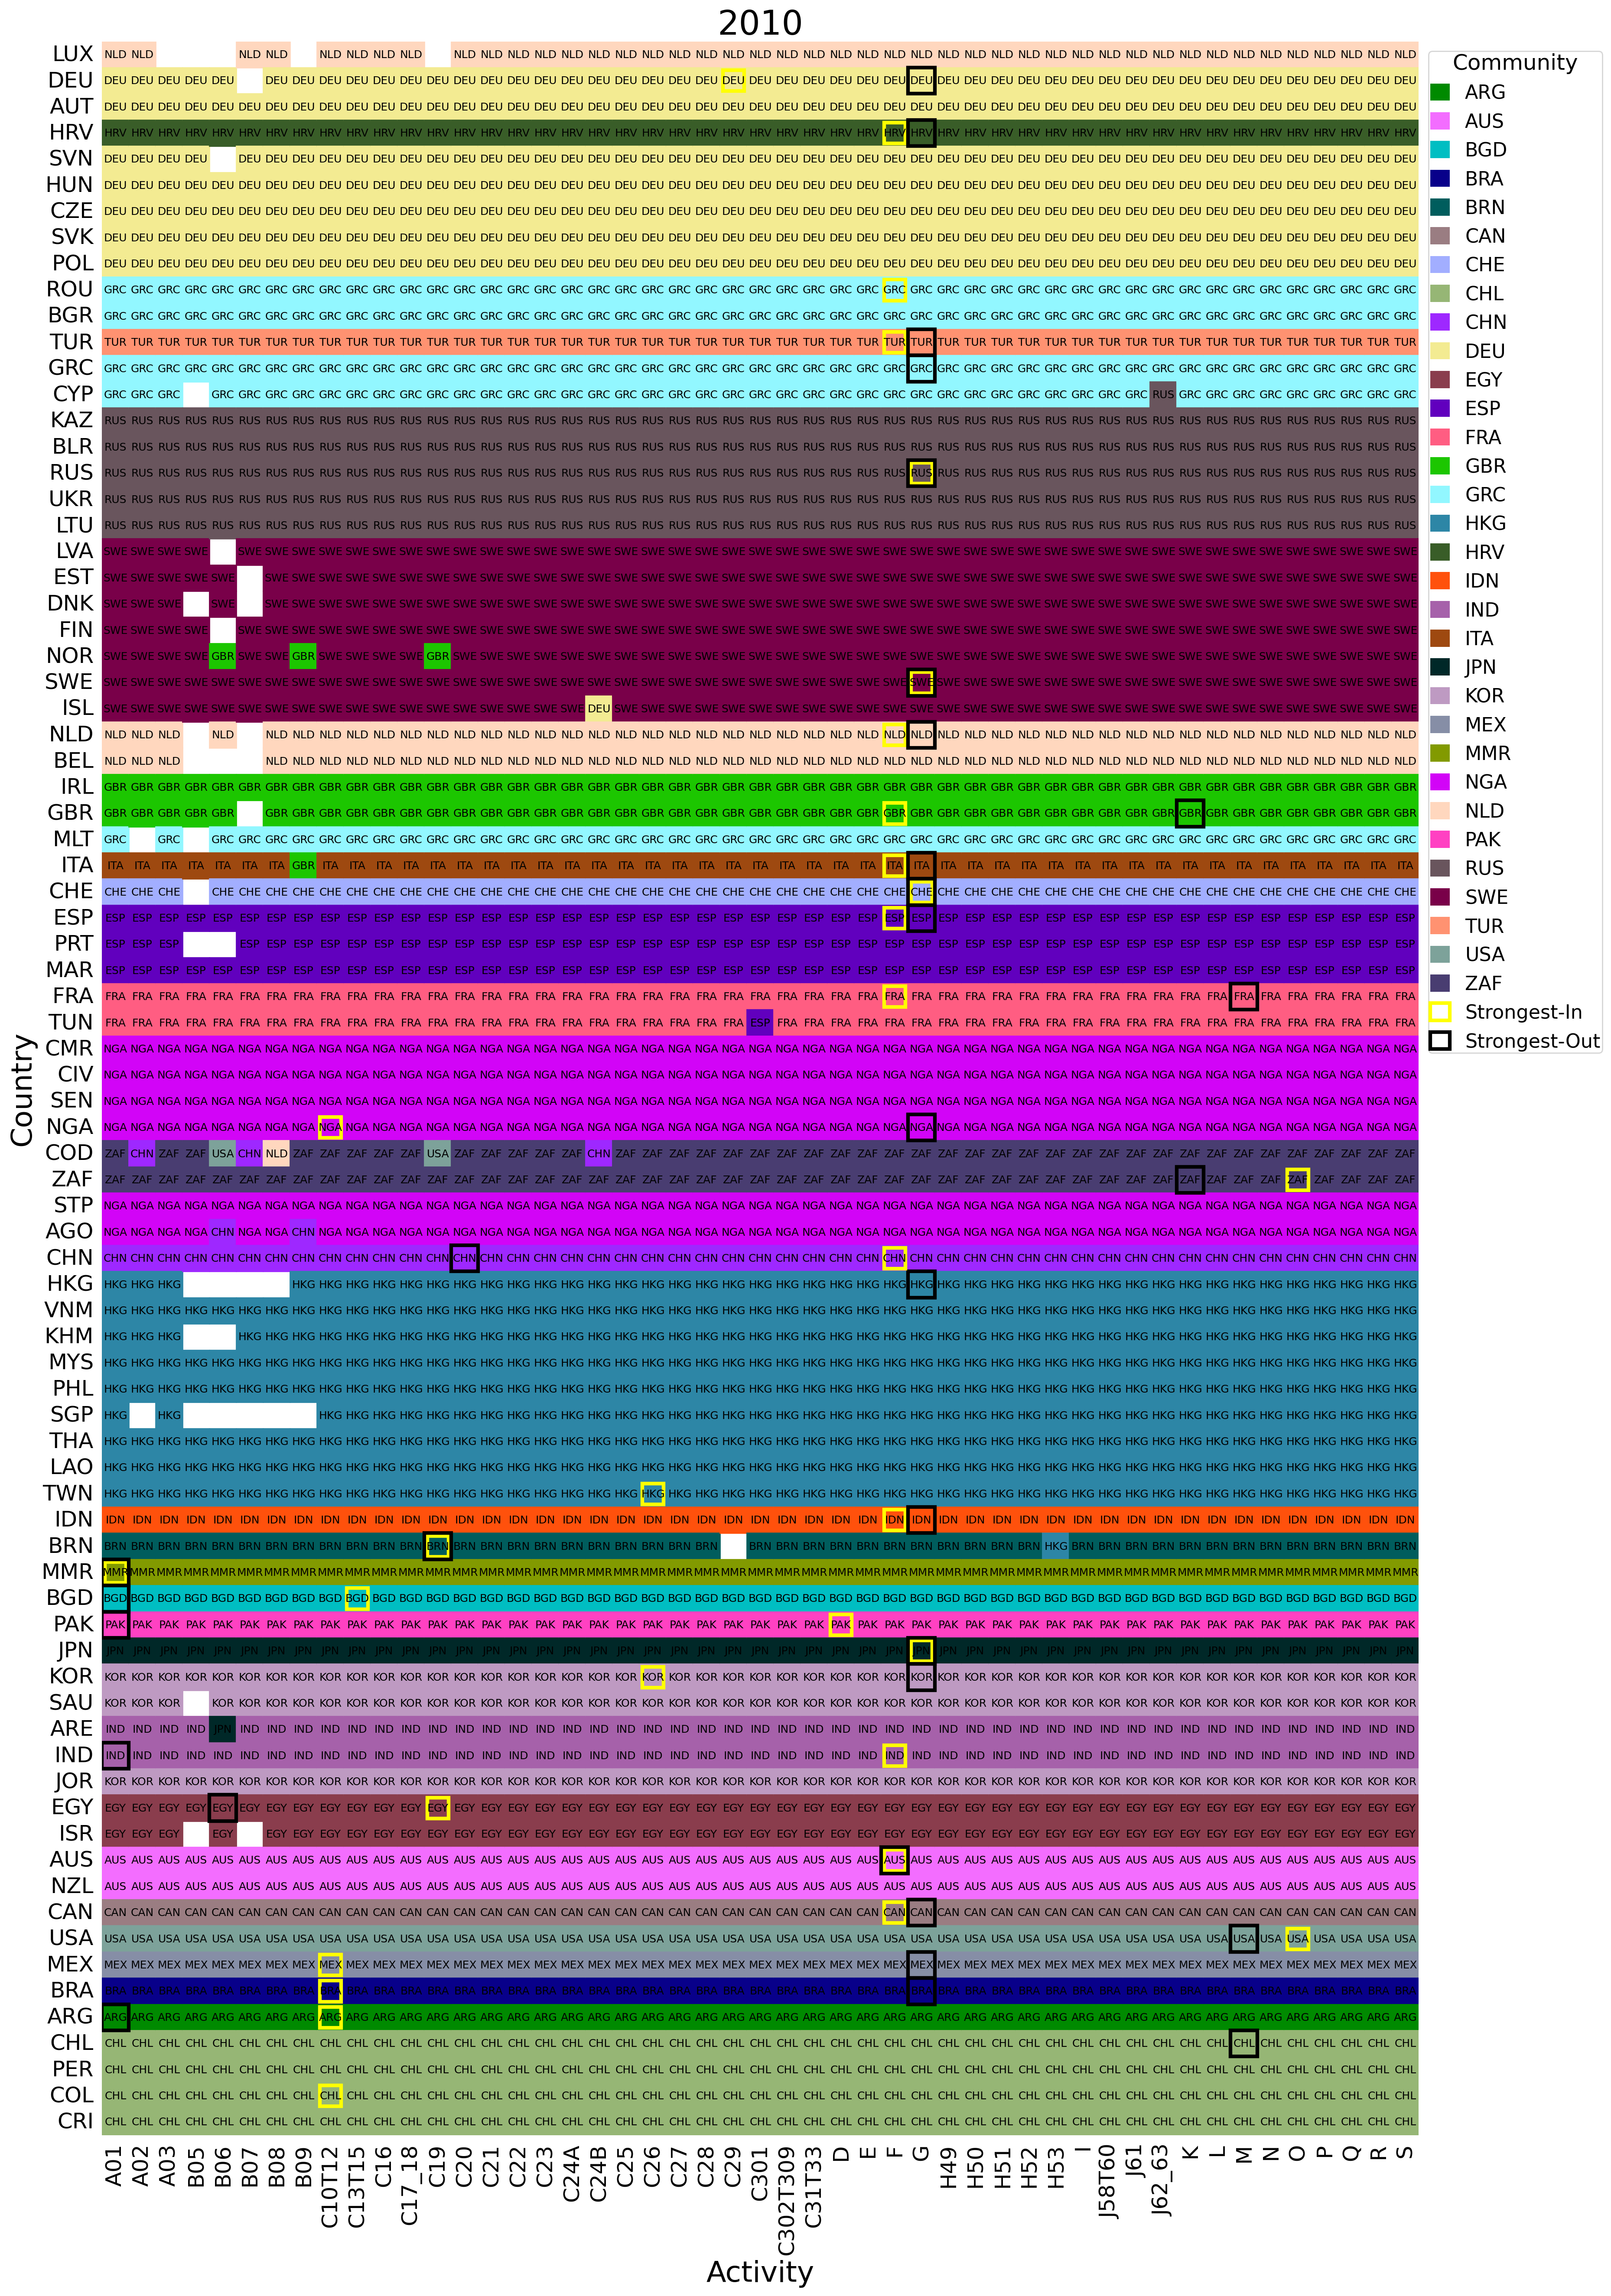
\includegraphics[width=\linewidth]{2010_communities.png}
	\caption{Resultados de la detección de comunidades en 2010.}
	\label{Fig_2010_comunidades}
\end{figure}

\begin{figure}[H]
	\centering
	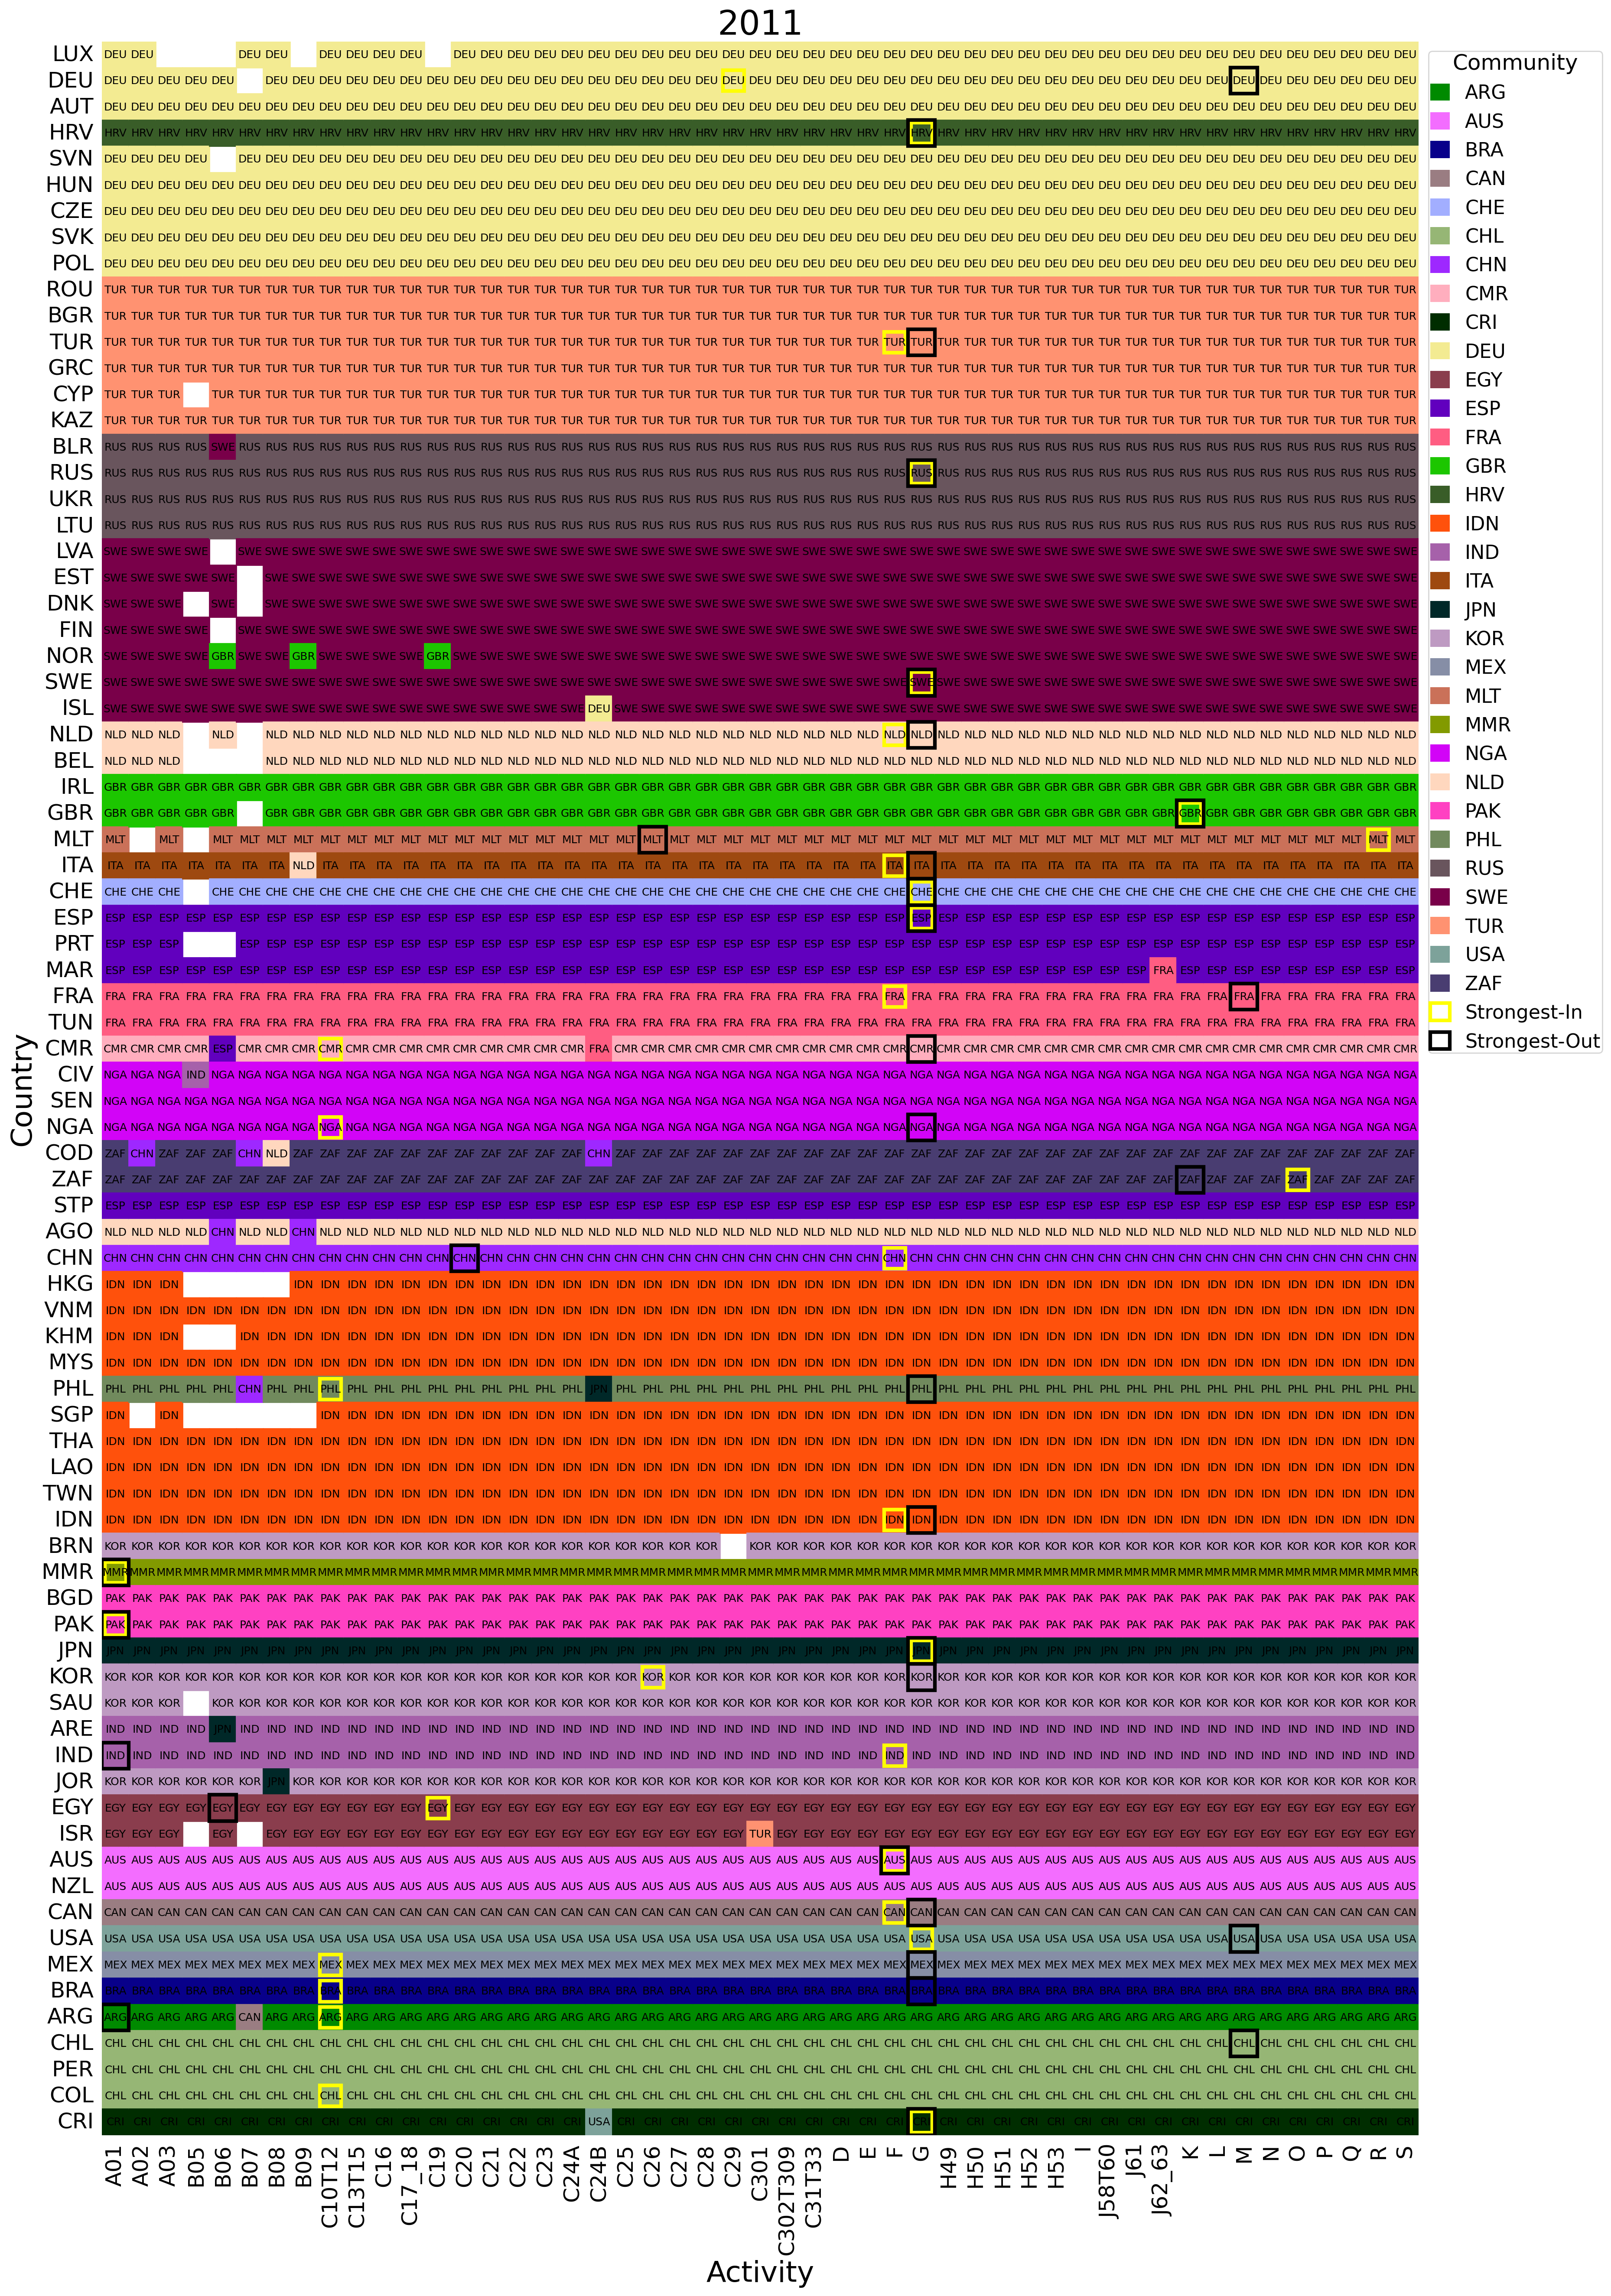
\includegraphics[width=\linewidth]{2011_communities.png}
	\caption{Resultados de la detección de comunidades en 2011.}
	\label{Fig_2011_comunidades}
\end{figure}

\begin{figure}[H]
	\centering
	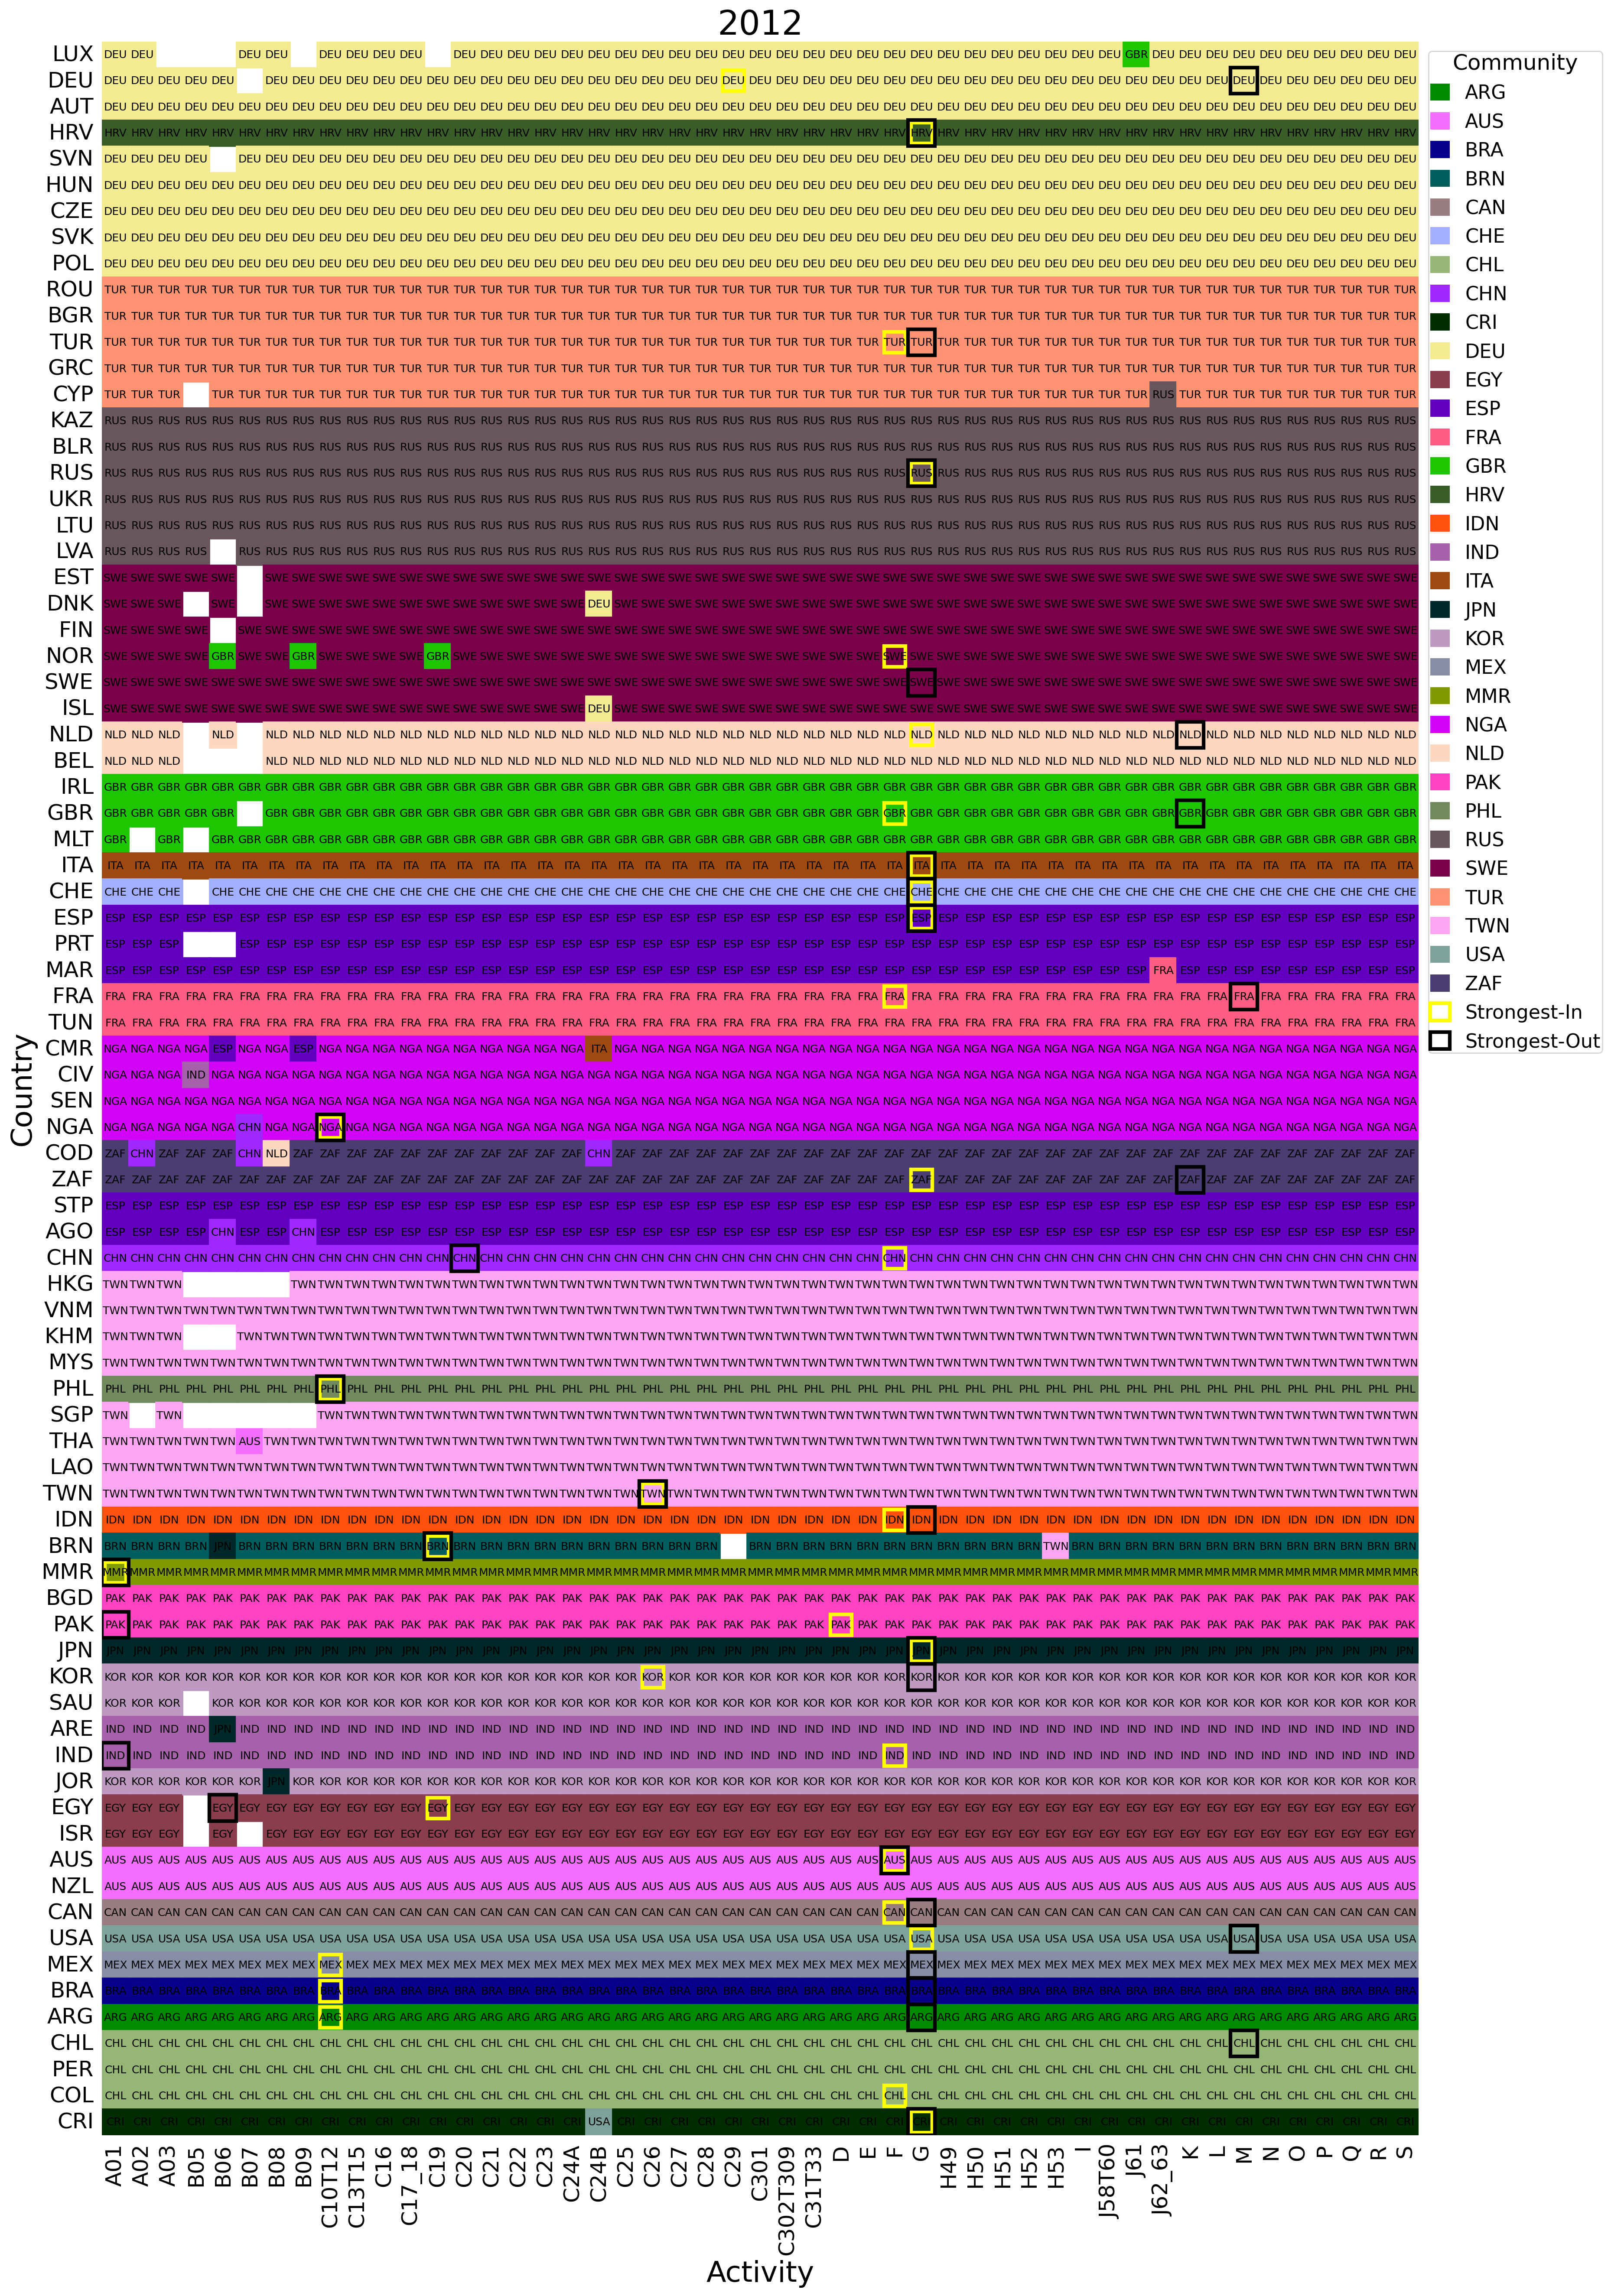
\includegraphics[width=\linewidth]{2012_communities.png}
	\caption{Resultados de la detección de comunidades en 2012.}
	\label{Fig_2012_comunidades}
\end{figure}

\begin{figure}[H]
	\centering
	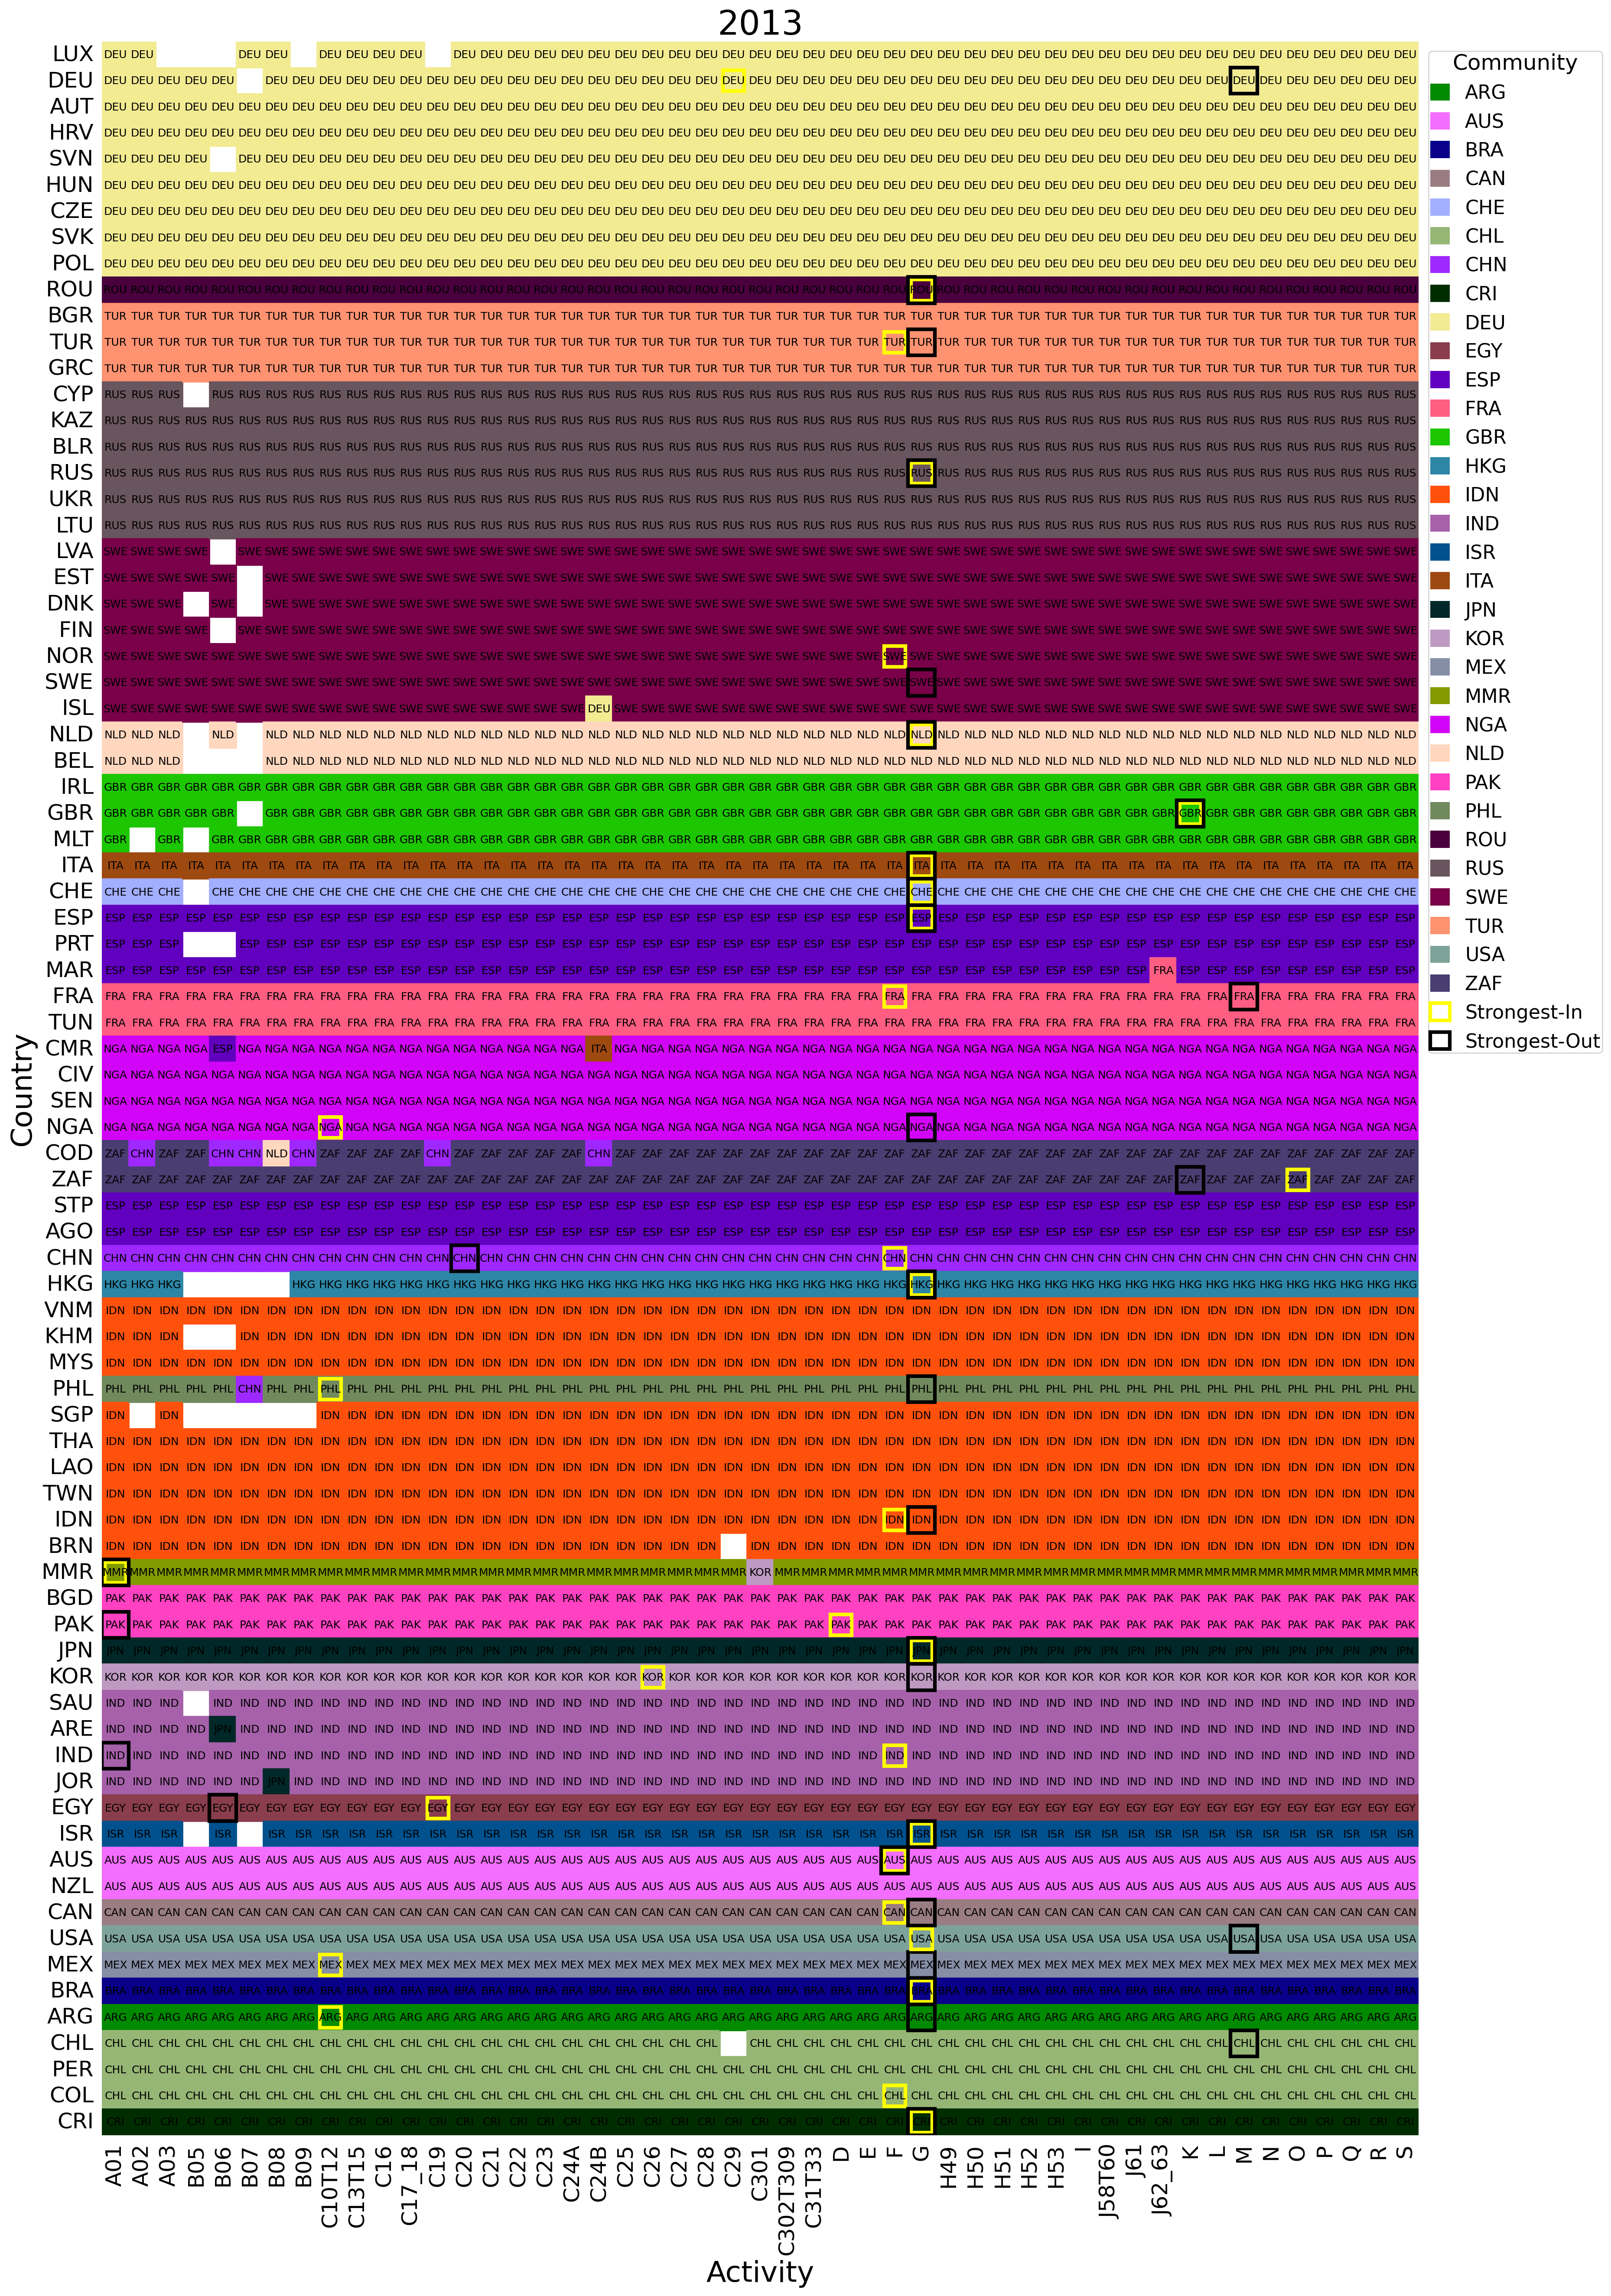
\includegraphics[width=\linewidth]{2013_communities.png}
	\caption{Resultados de la detección de comunidades en 2013.}
	\label{Fig_2013_comunidades}
\end{figure}

\begin{figure}[H]
	\centering
	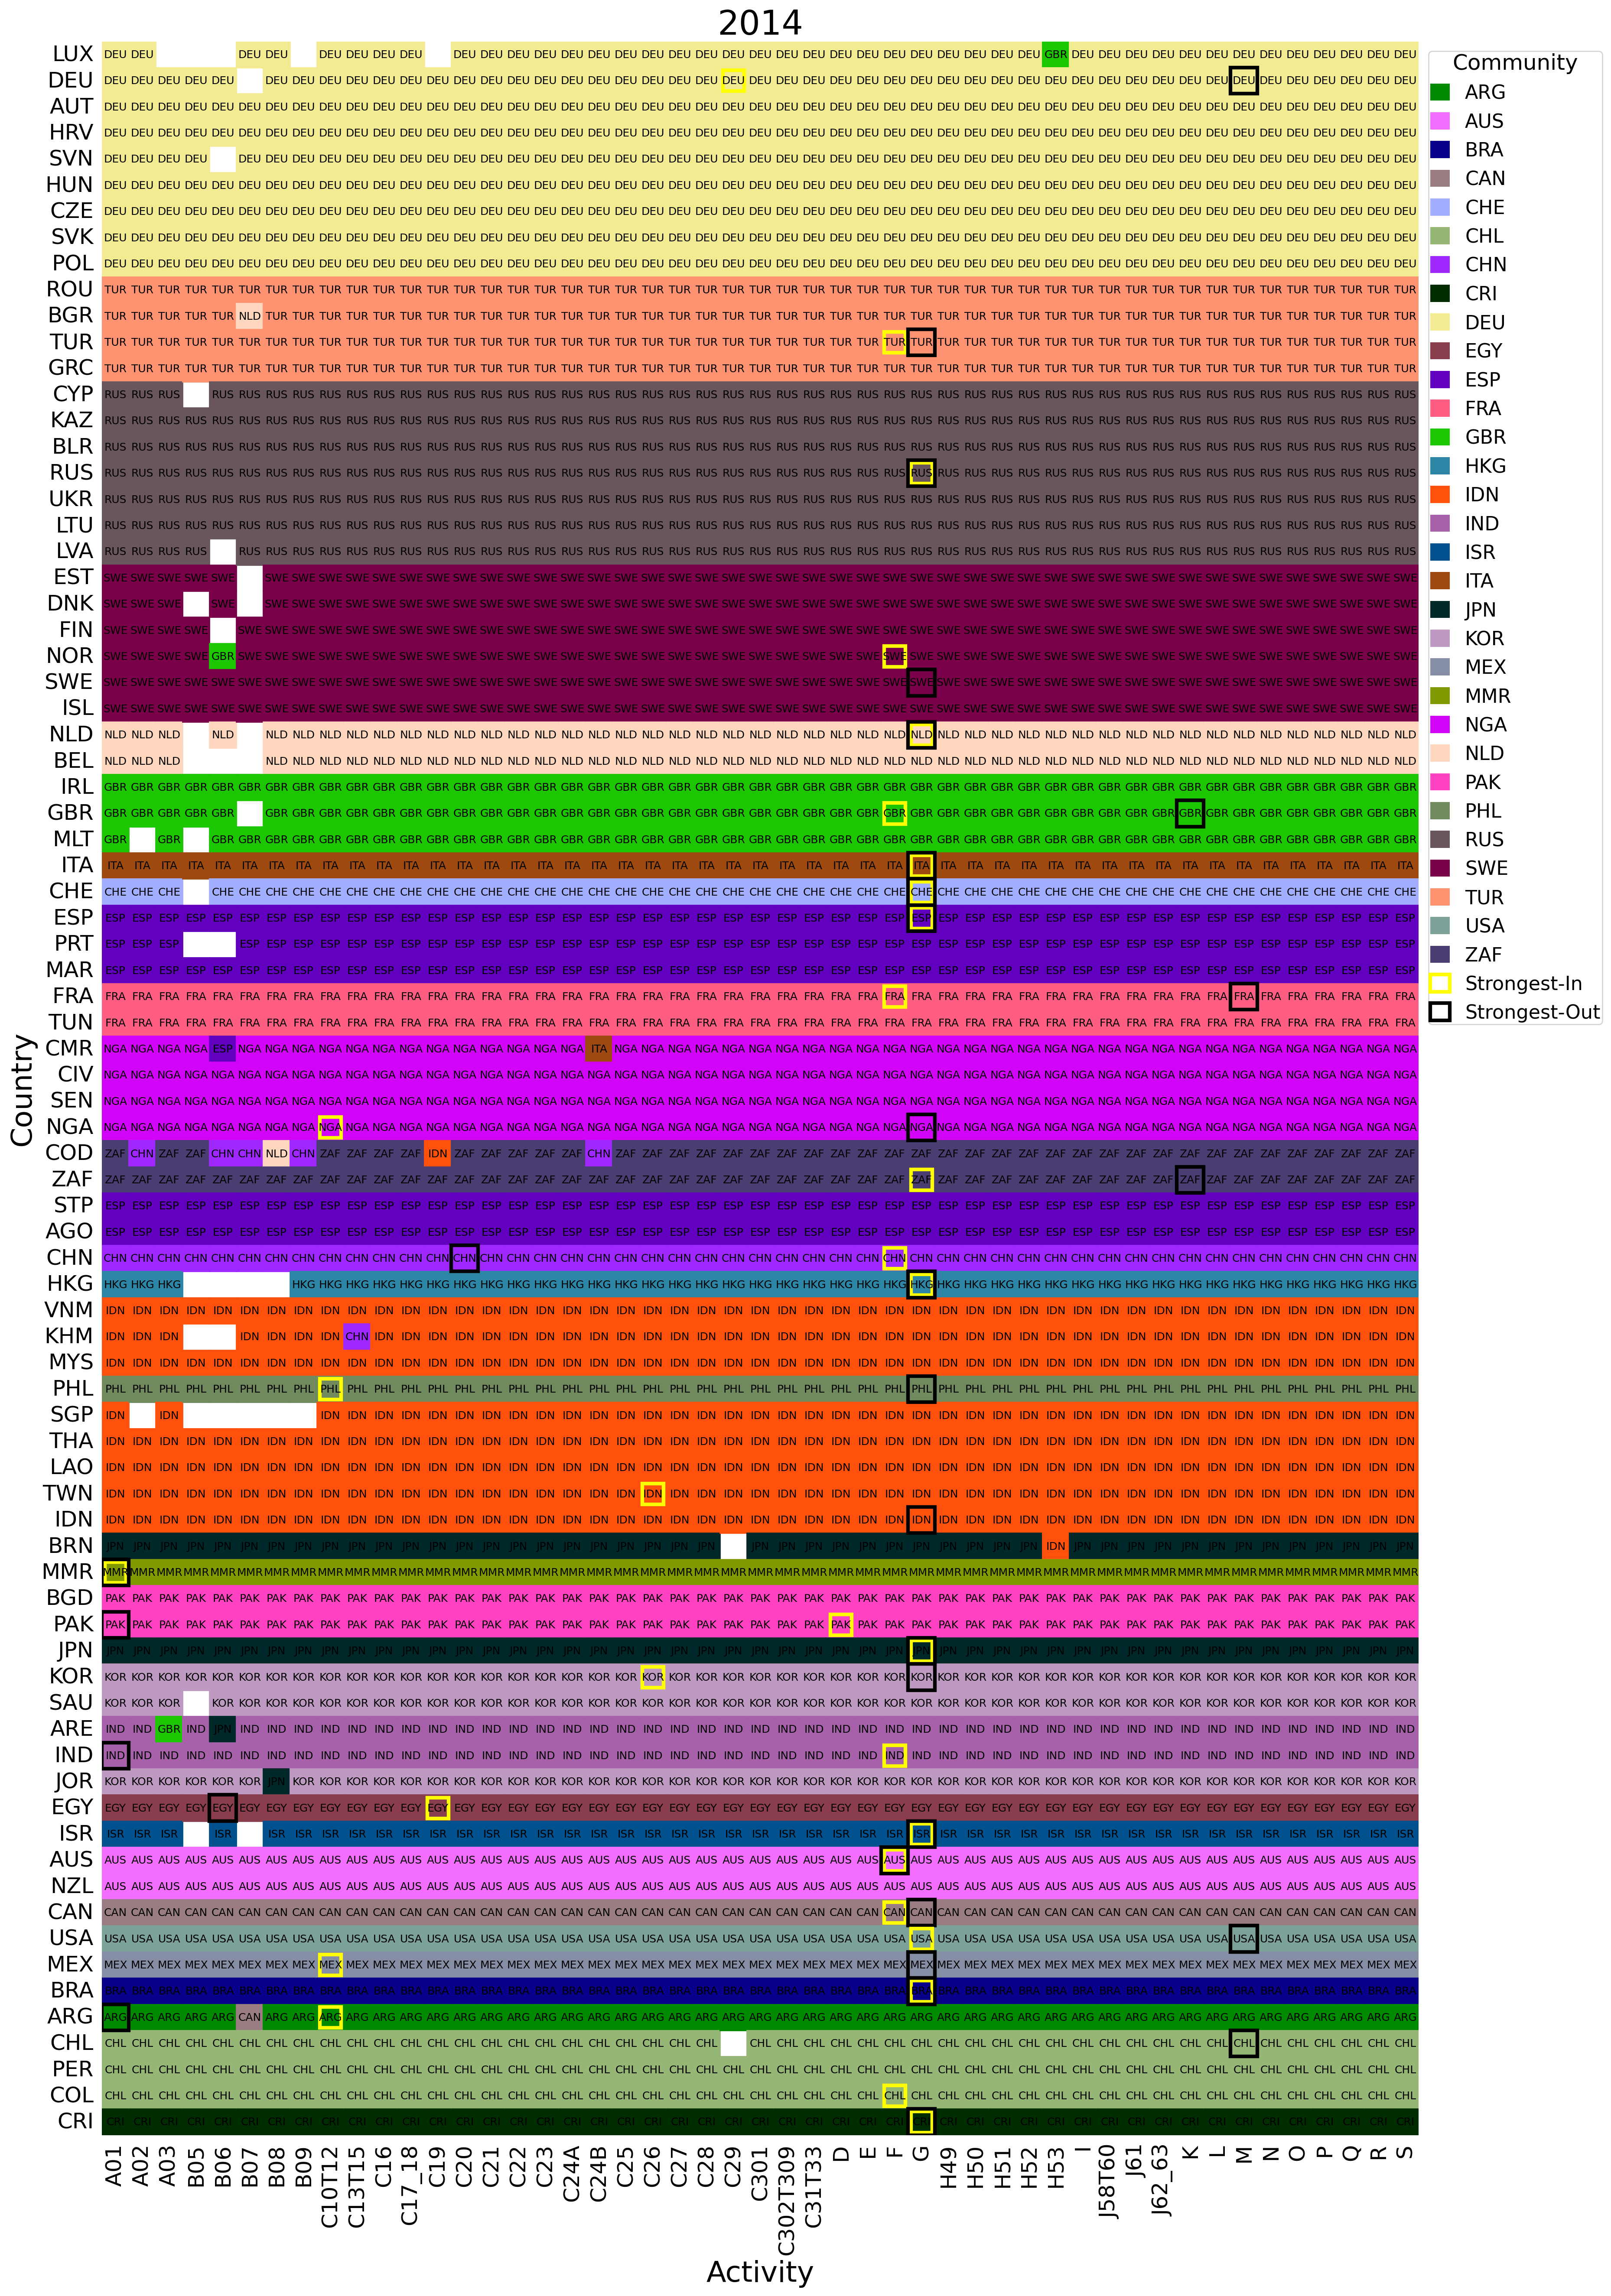
\includegraphics[width=\linewidth]{2014_communities.png}
	\caption{Resultados de la detección de comunidades en 2014.}
	\label{Fig_2014_comunidades}
\end{figure}

\begin{figure}[H]
	\centering
	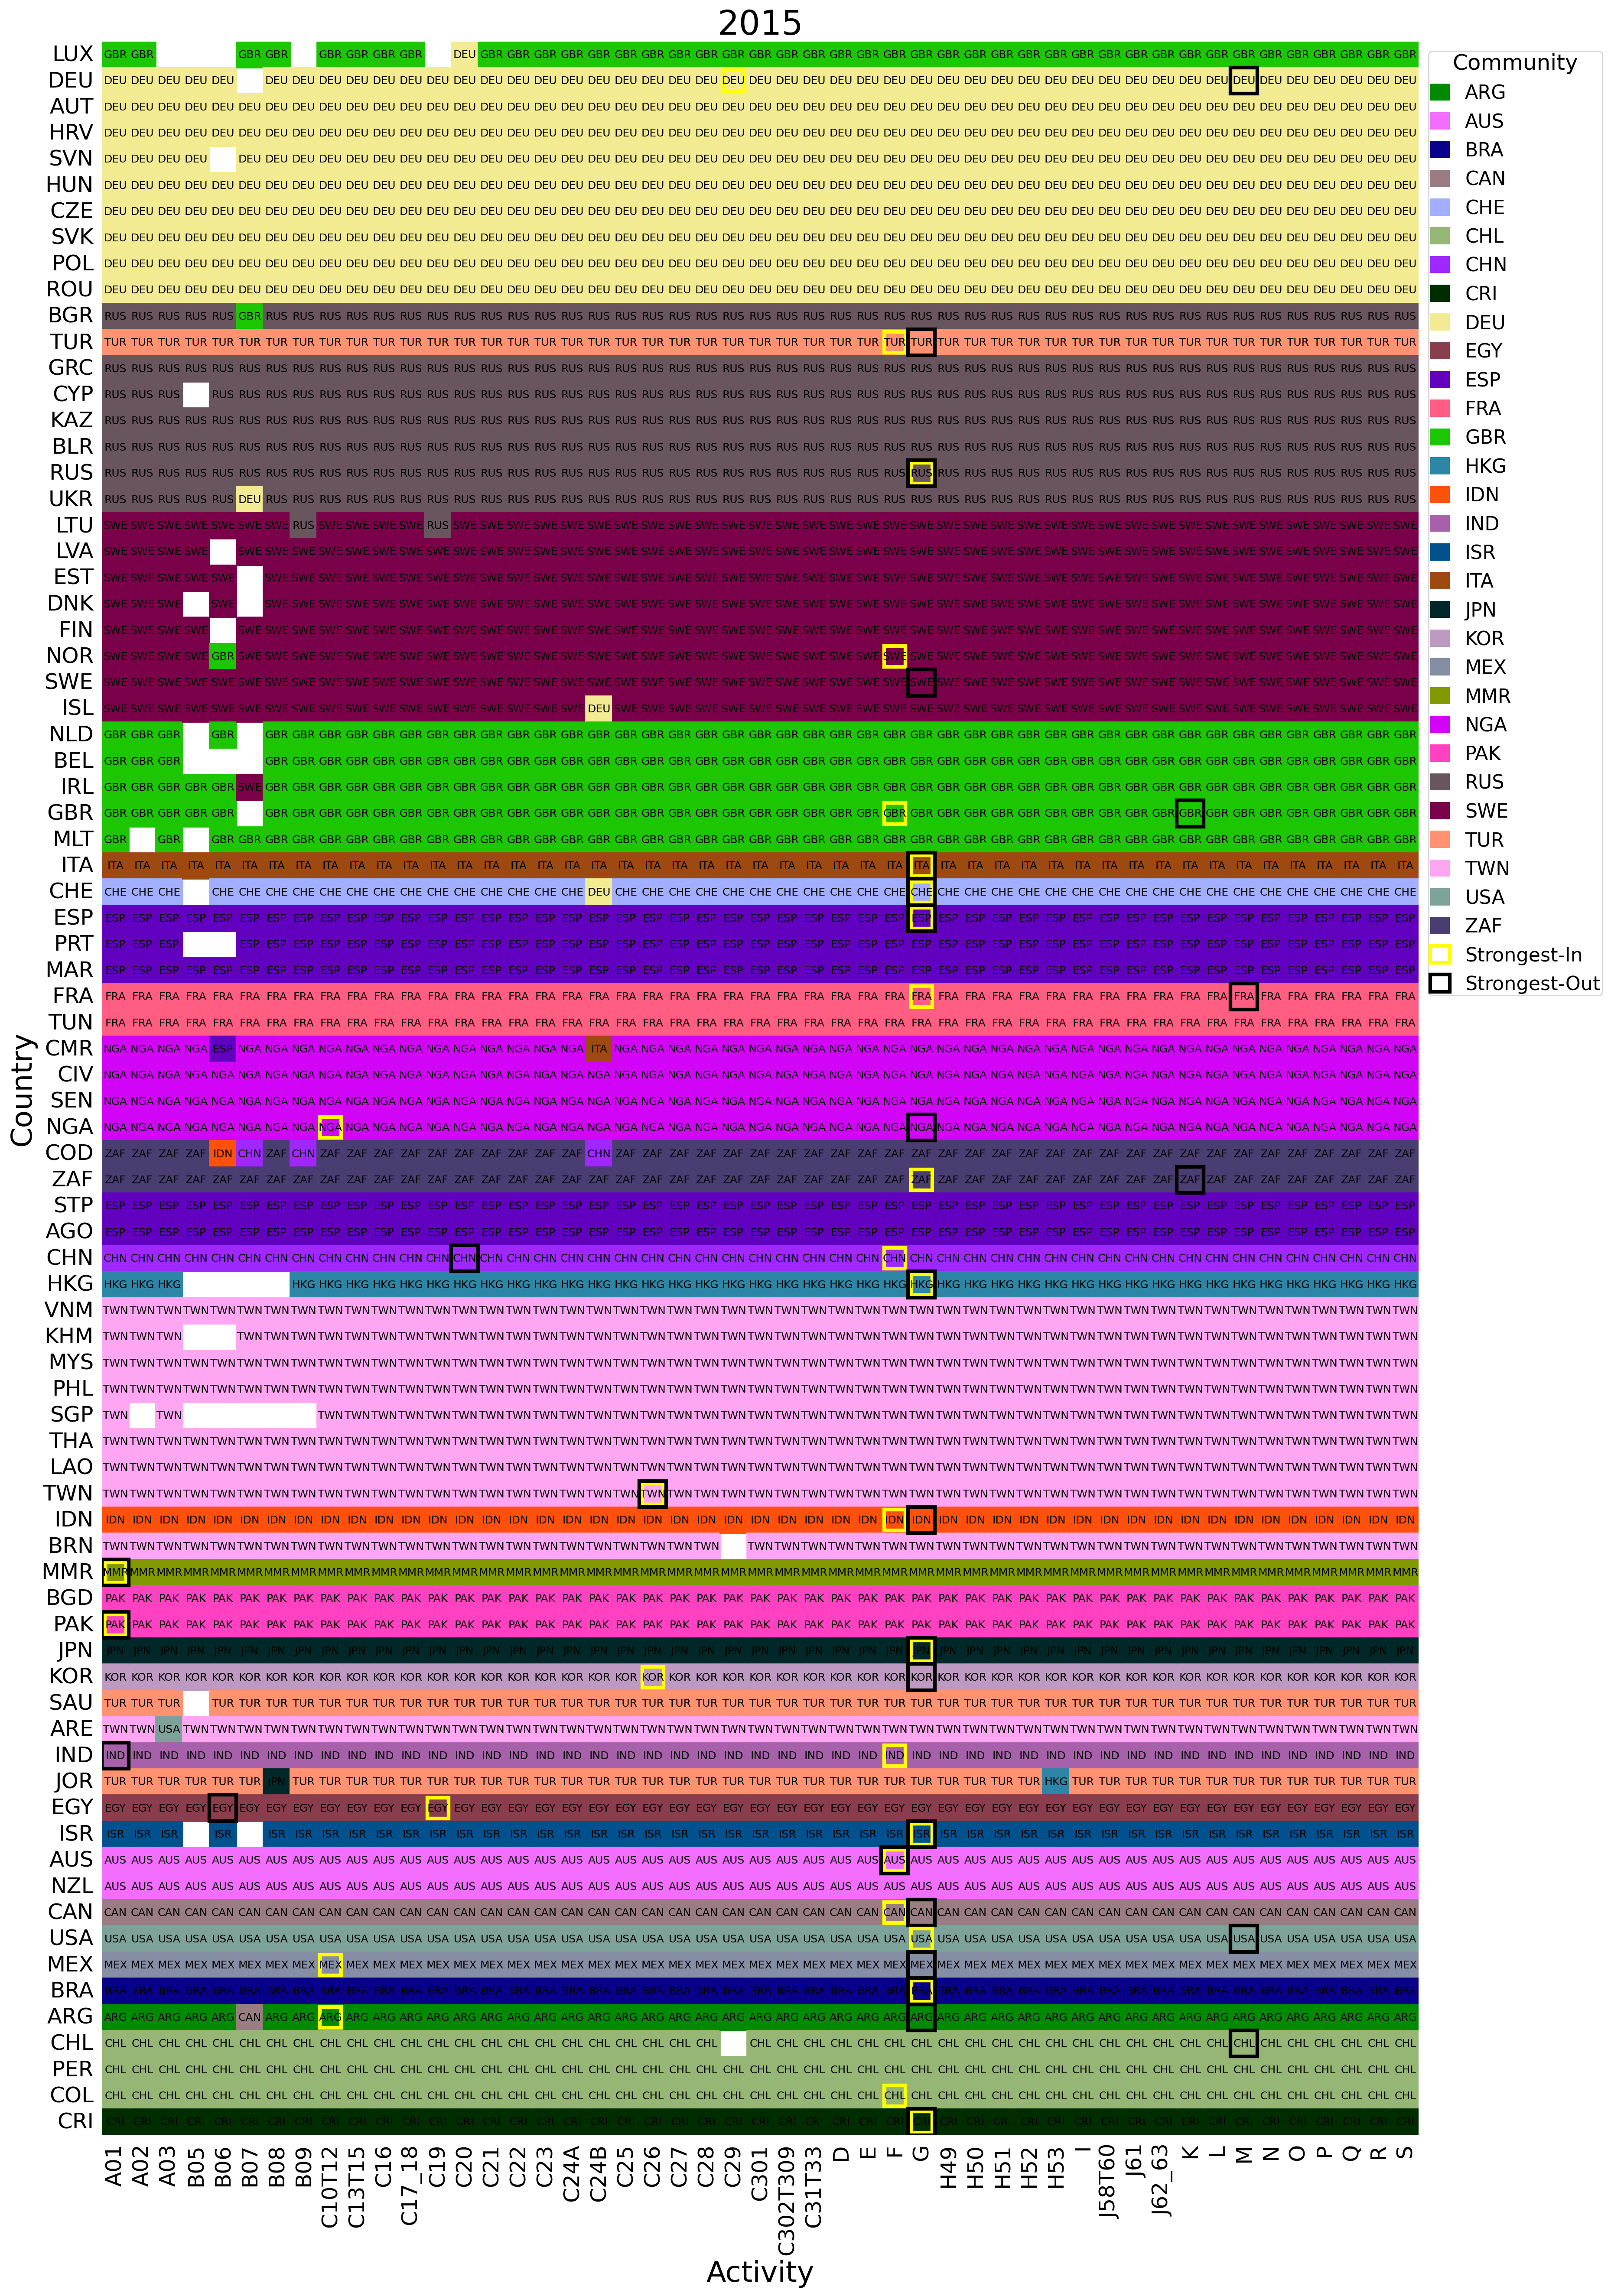
\includegraphics[width=\linewidth]{2015_communities.png}
	\caption{Resultados de la detección de comunidades en 2015.}
	\label{Fig_2015_comunidades}
\end{figure}

\begin{figure}[H]
	\centering
	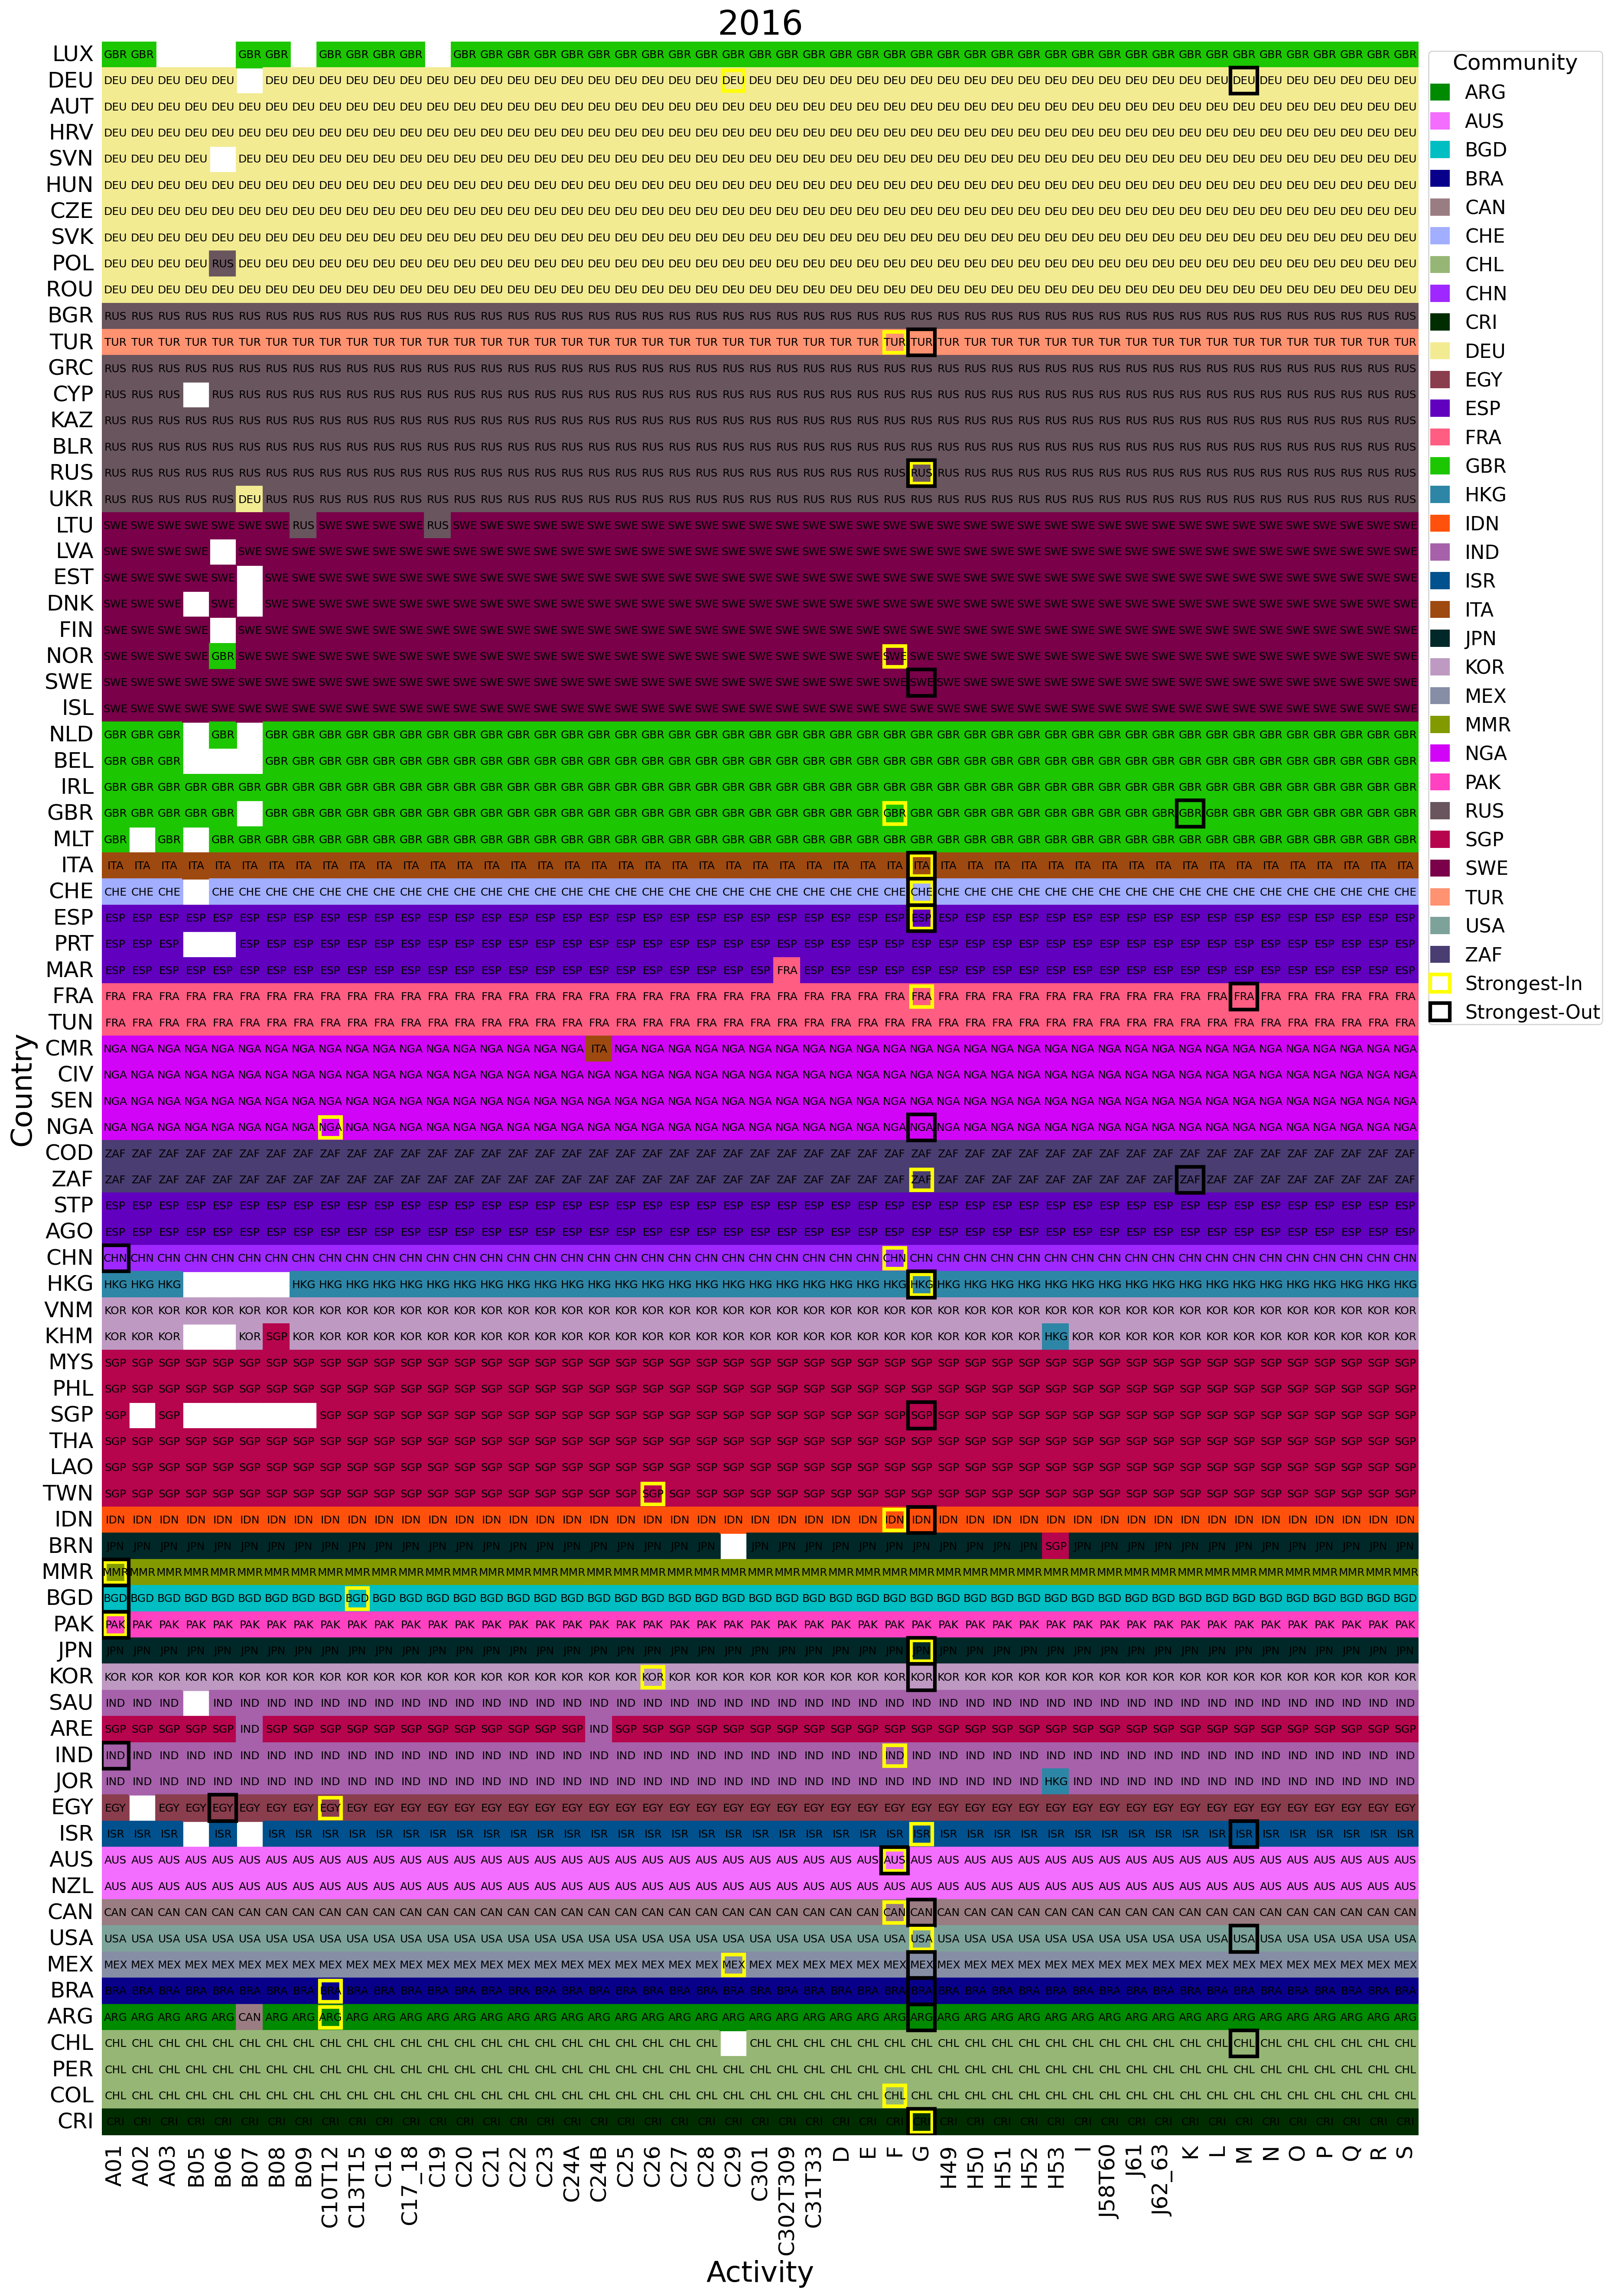
\includegraphics[width=\linewidth]{2016_communities.png}
	\caption{Resultados de la detección de comunidades en 2016.}
	\label{Fig_2016_comunidades}
\end{figure}

\begin{figure}[H]
	\centering
	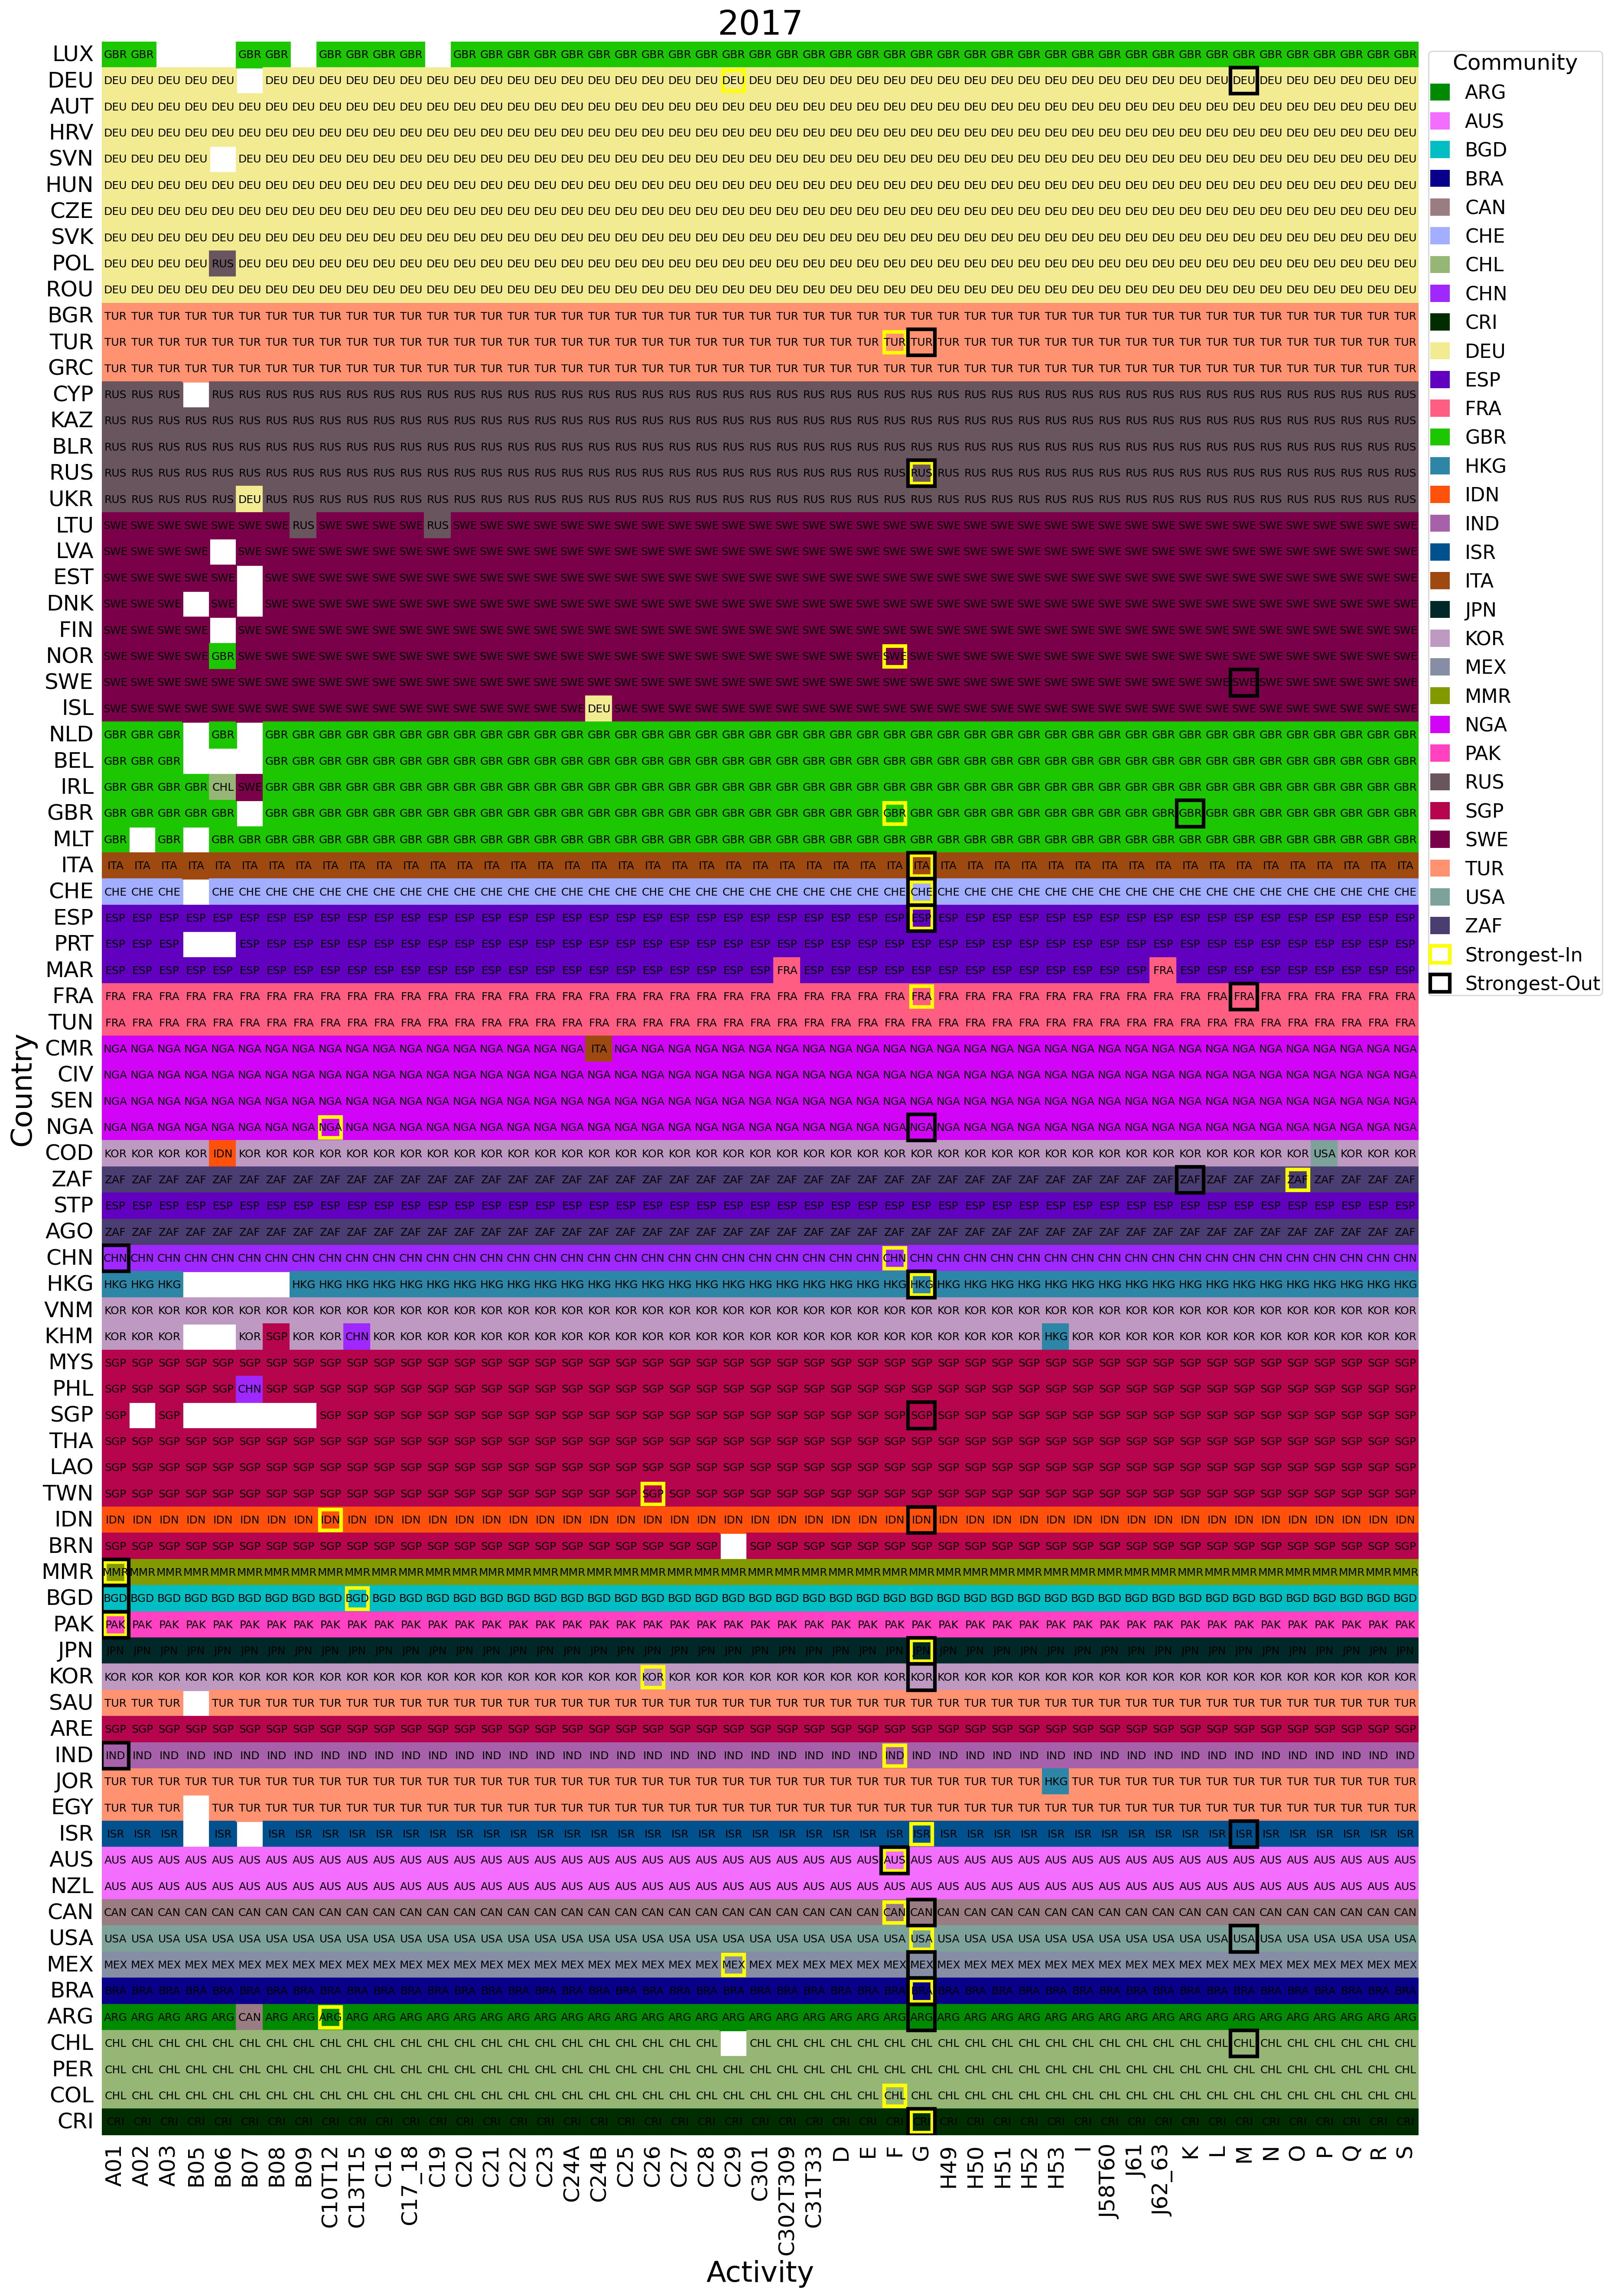
\includegraphics[width=\linewidth]{2017_communities.png}
	\caption{Resultados de la detección de comunidades en 2017.}
	\label{Fig_2017_comunidades}
\end{figure}

\begin{figure}[H]
	\centering
	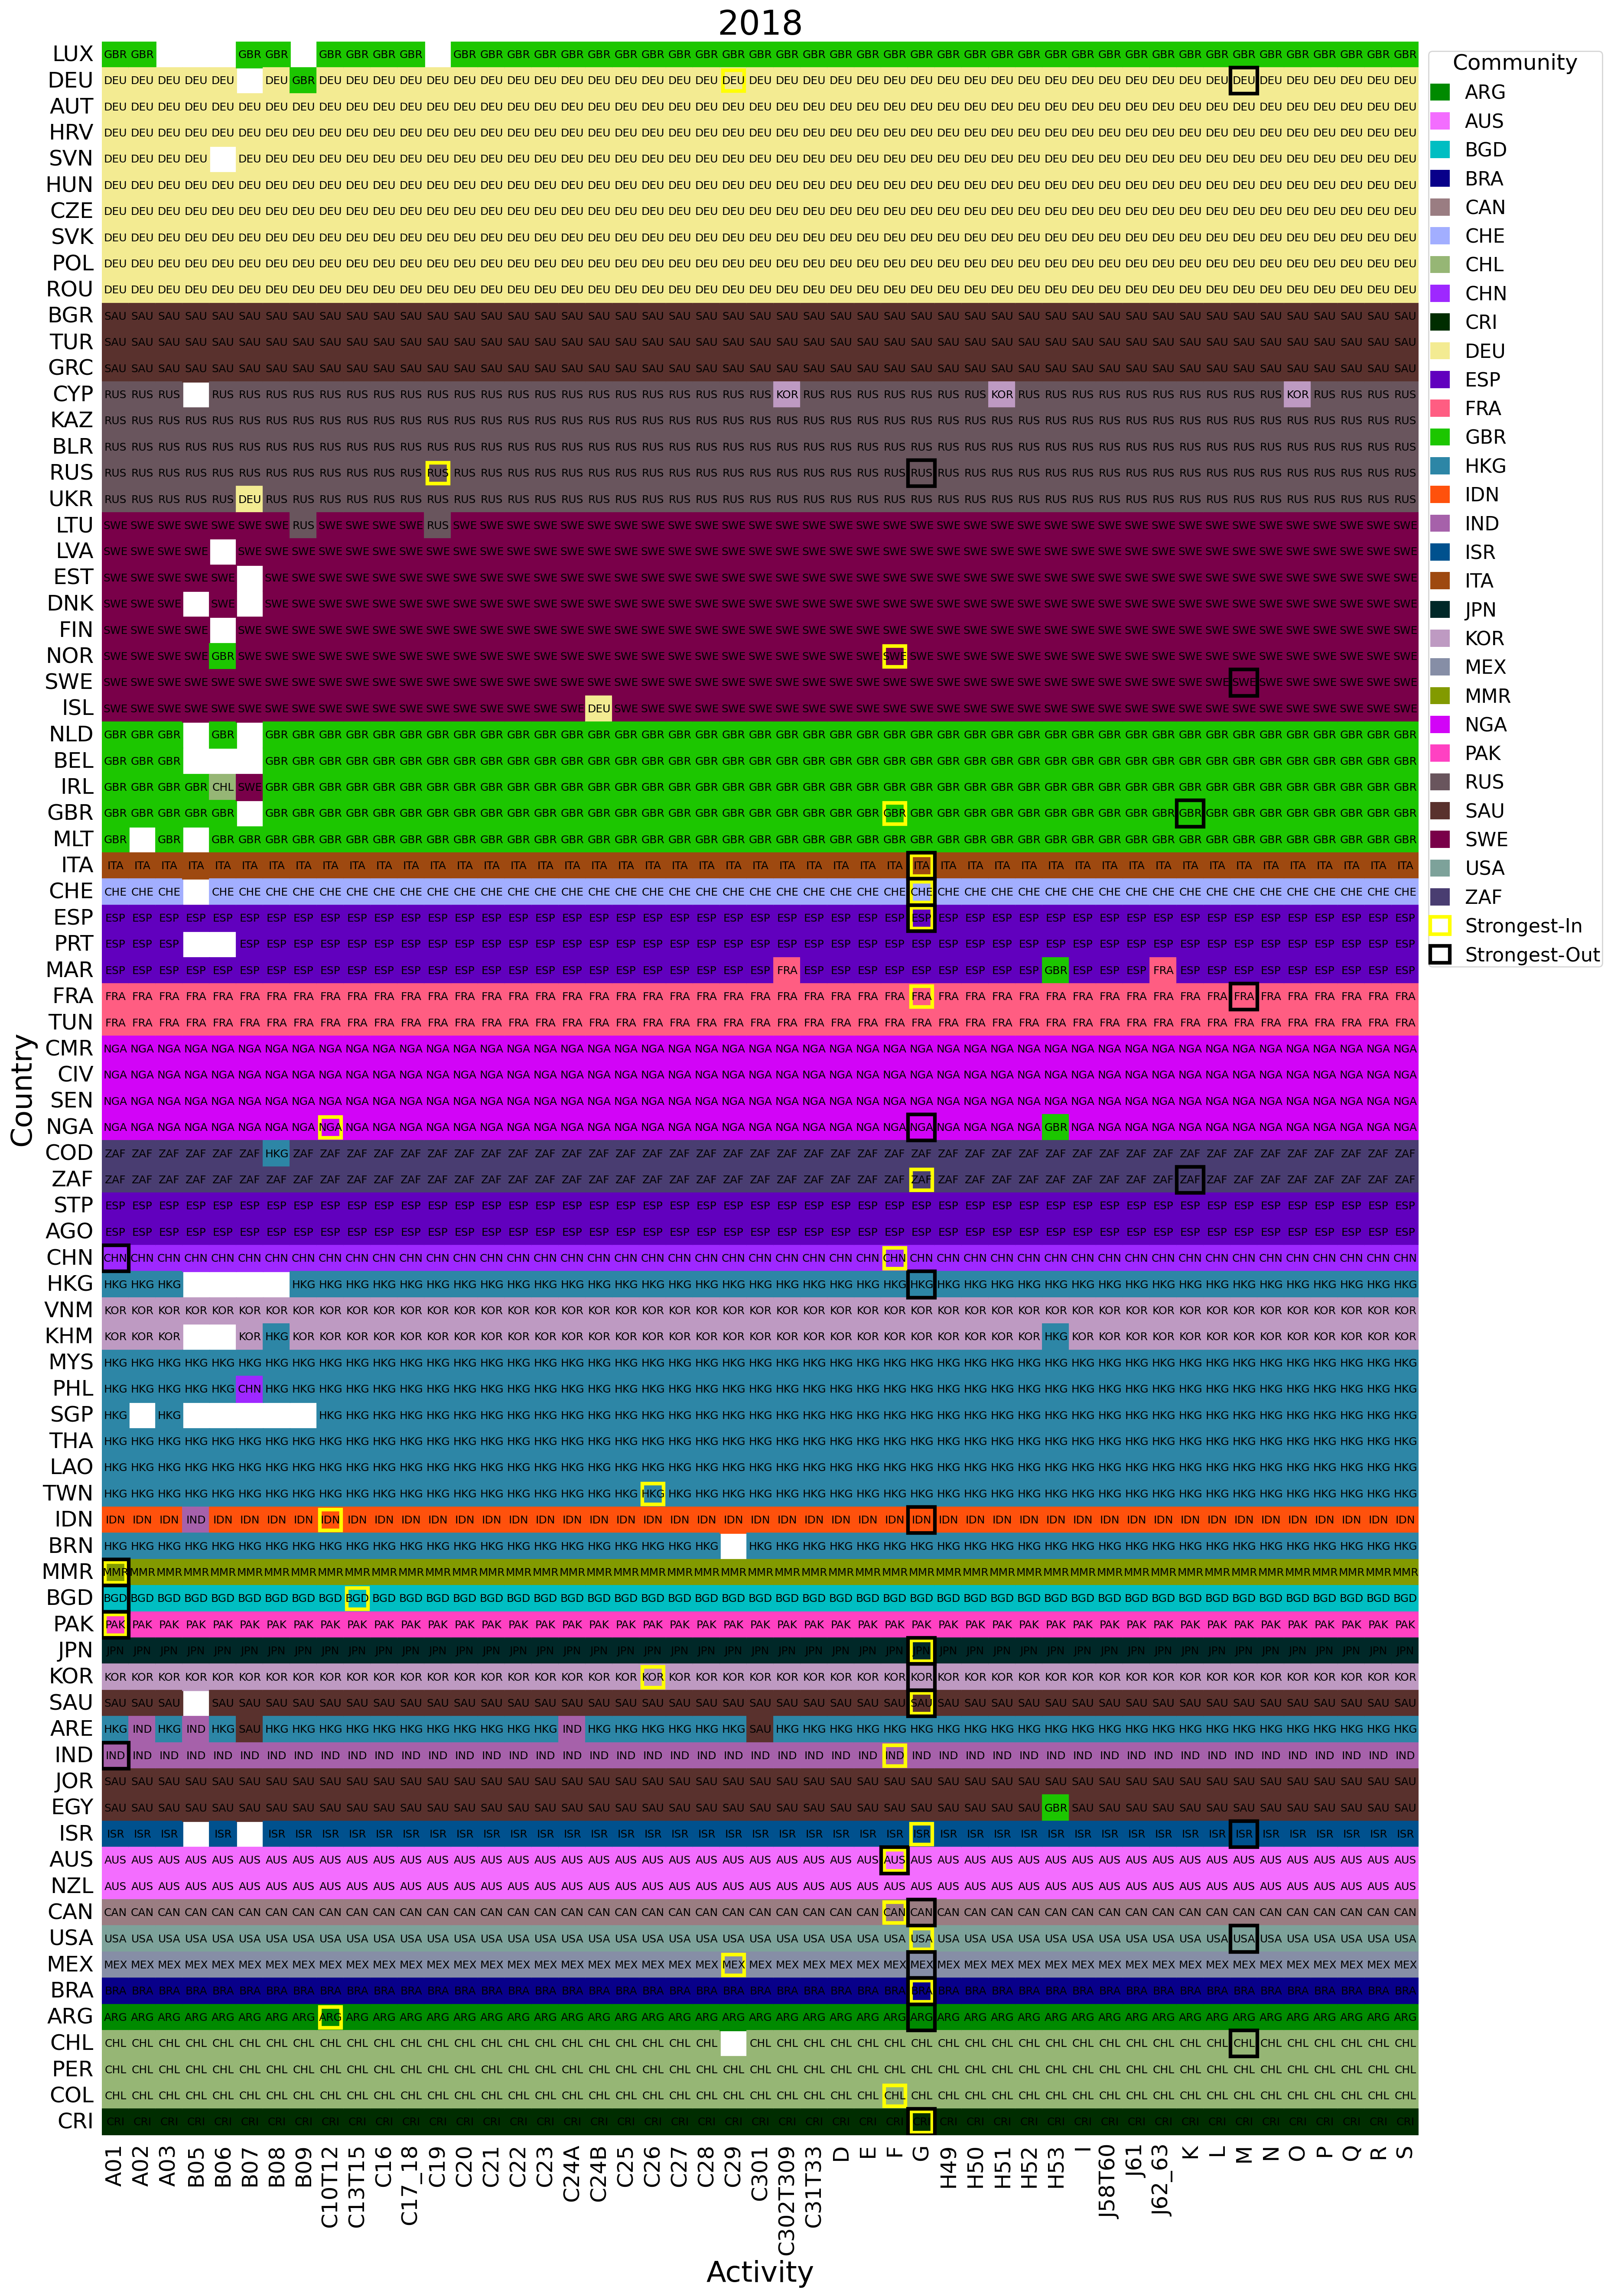
\includegraphics[width=\linewidth]{2018_communities.png}
	\caption{Resultados de la detección de comunidades en 2018.}
	\label{Fig_2018_comunidades}
\end{figure}

\begin{figure}[H]
	\centering
	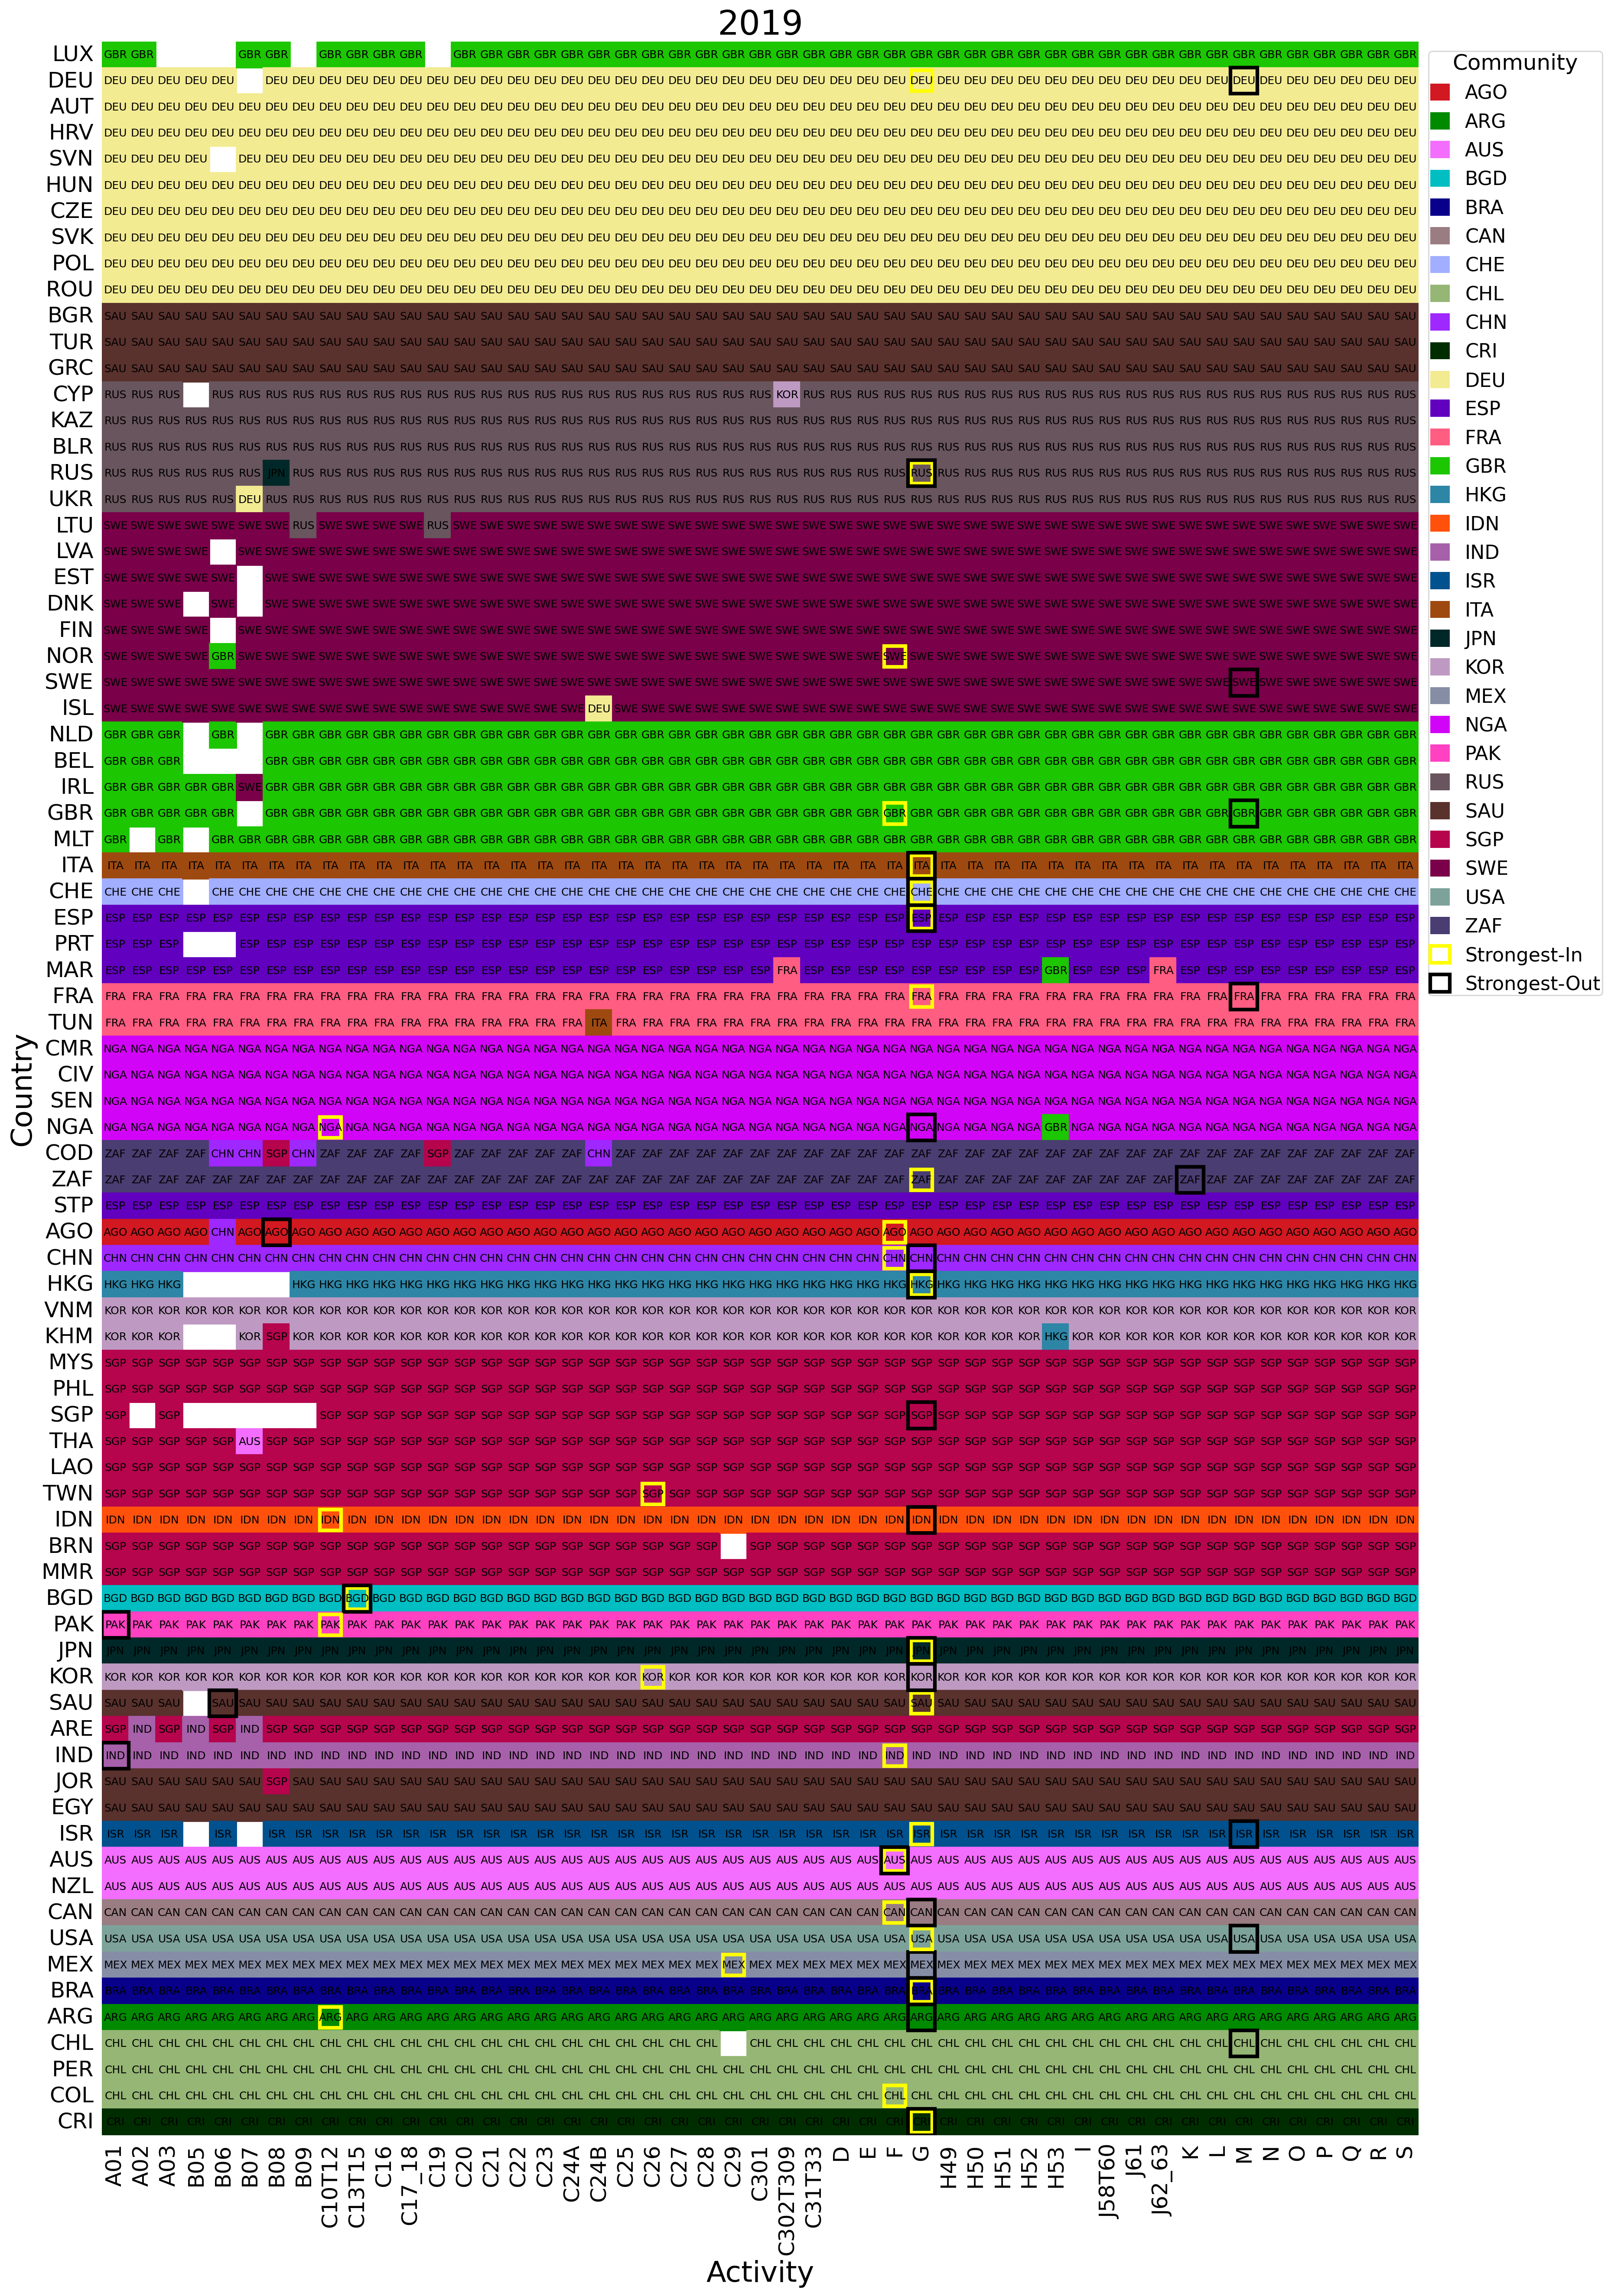
\includegraphics[width=\linewidth]{2019_communities.png}
	\caption{Resultados de la detección de comunidades en 2019.}
	\label{Fig_2019_comunidades}
\end{figure}


\begin{figure}[H]
	\centering
	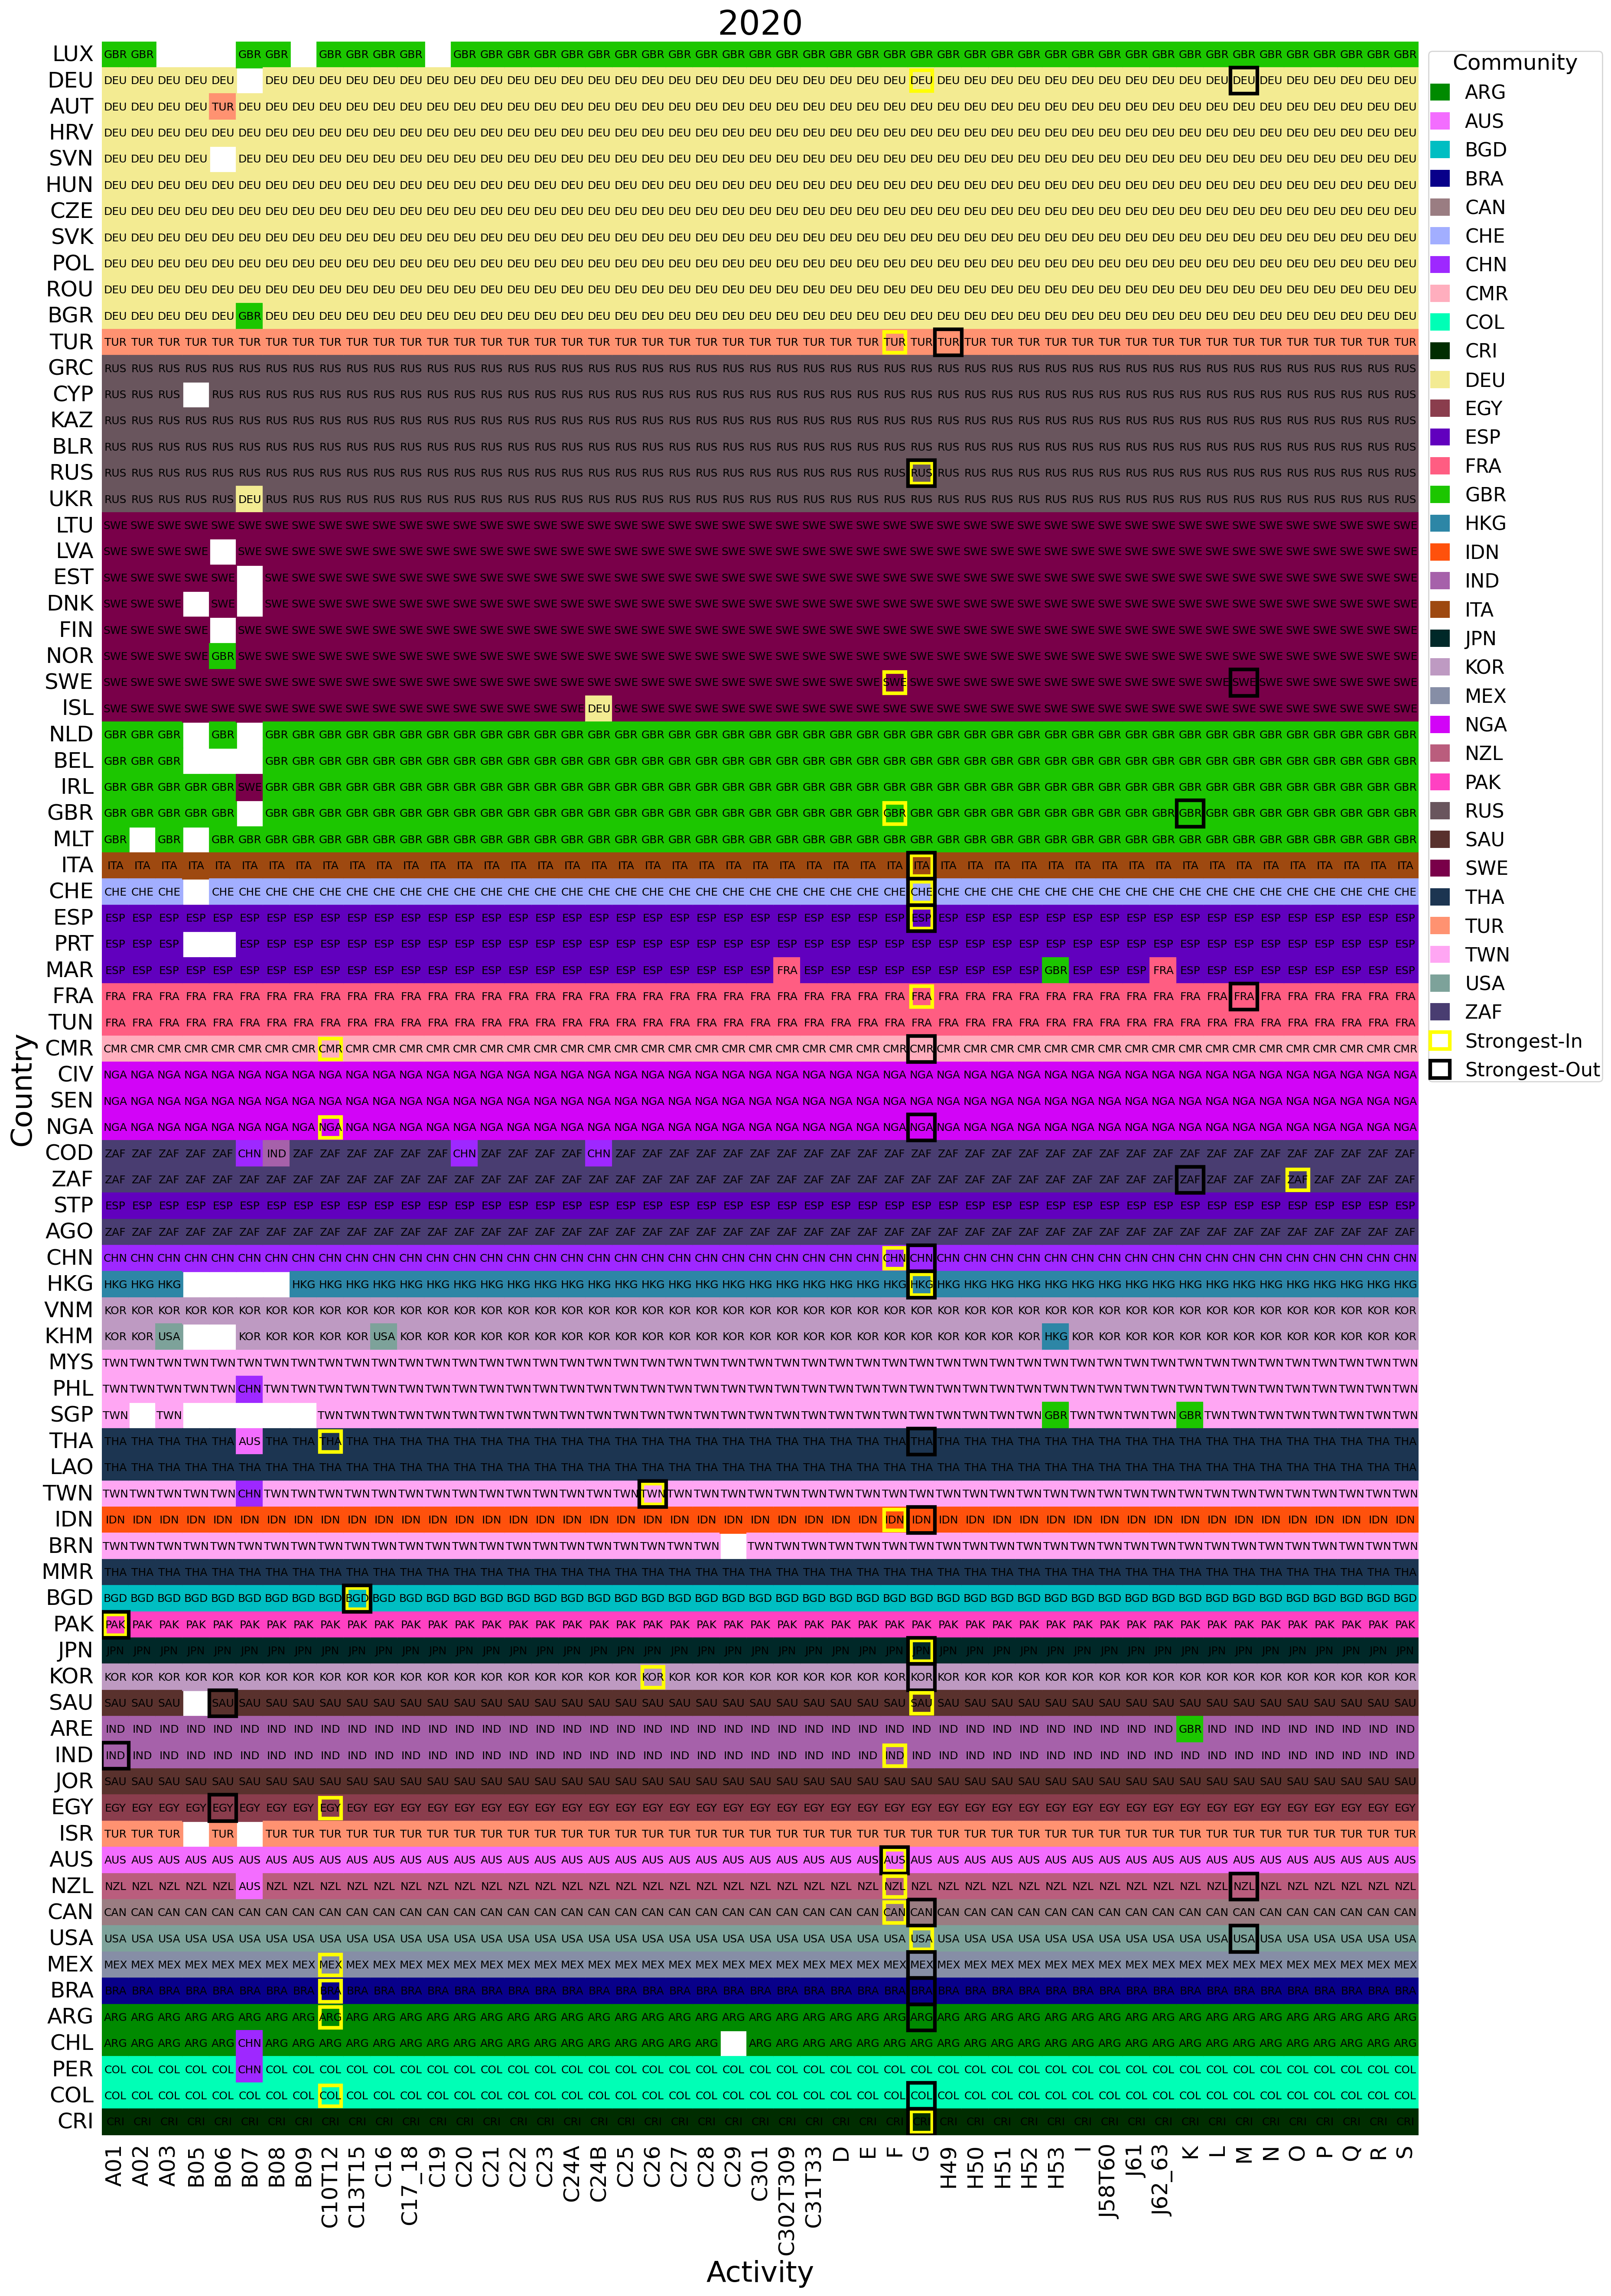
\includegraphics[width=\linewidth]{2020_communities.png}
	\caption{Resultados de la detección de comunidades en 2020.}
	\label{Fig_2020_comunidades}
\end{figure}


\begin{figure}[H]
	\centering
	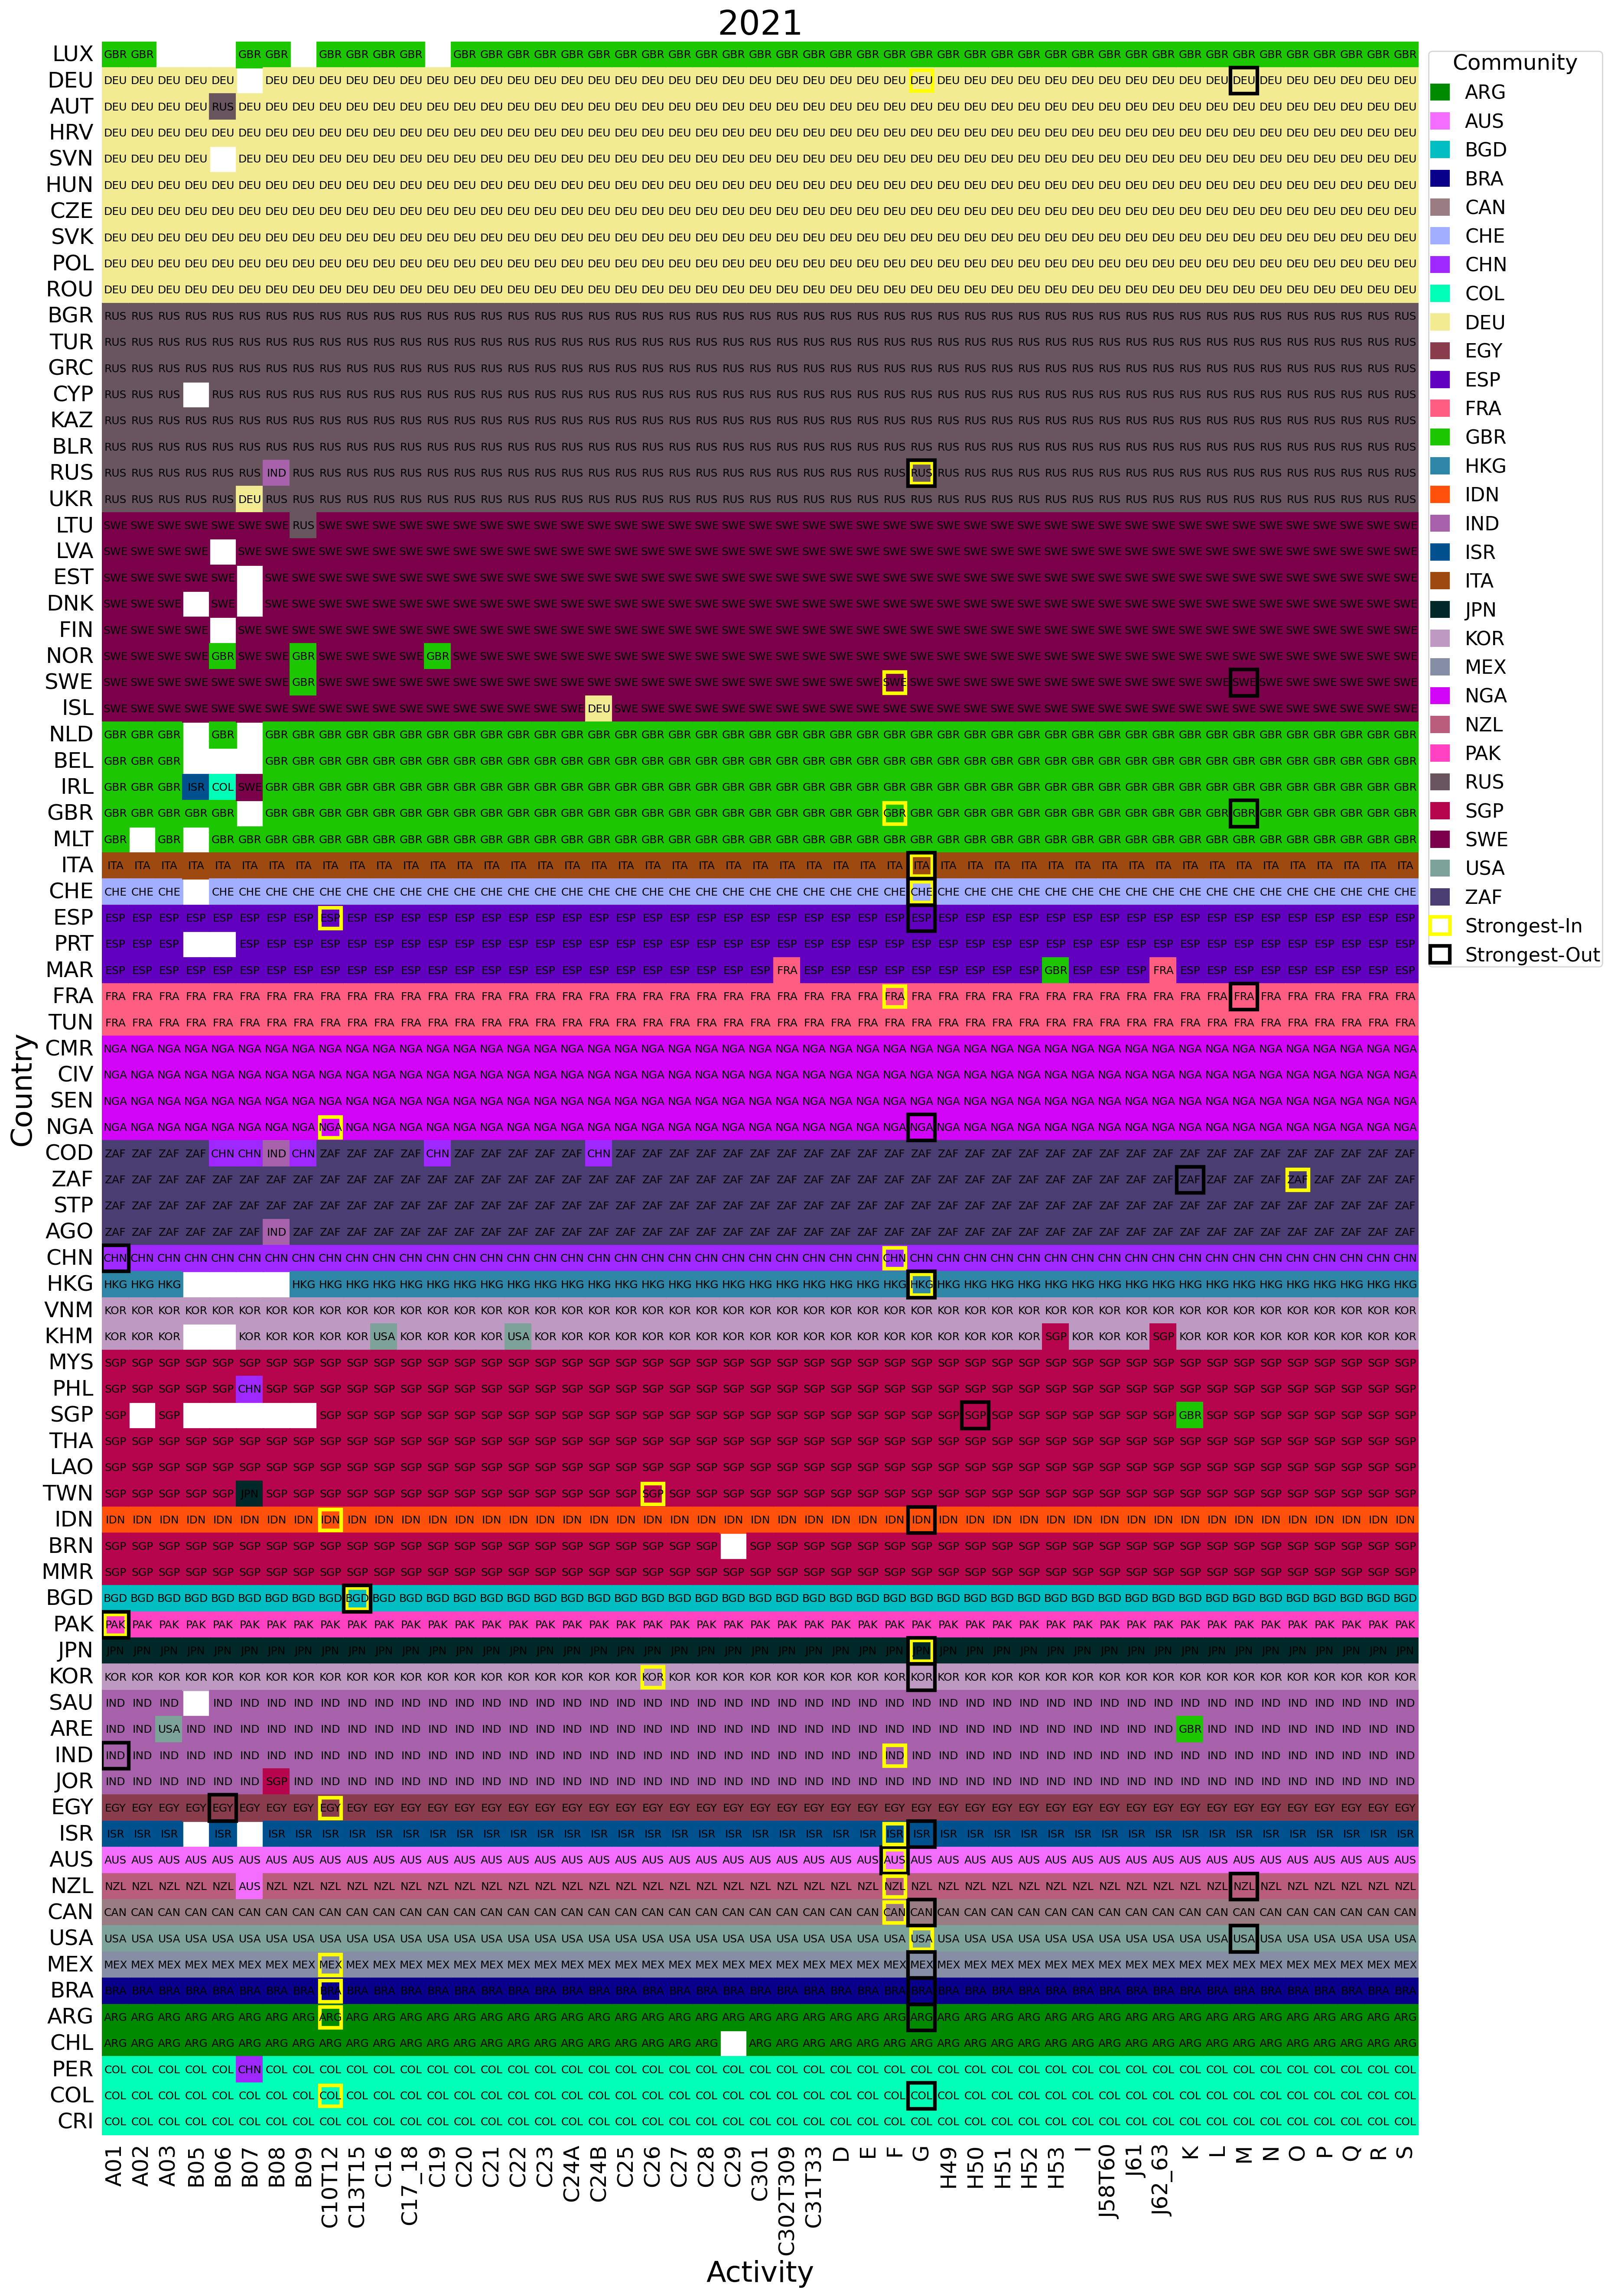
\includegraphics[width=\linewidth]{2021_communities.png}
	\caption{Resultados de la detección de comunidades en 2021.}
	\label{Fig_2021_comunidades}
\end{figure}


\begin{figure}[H]
	\centering
	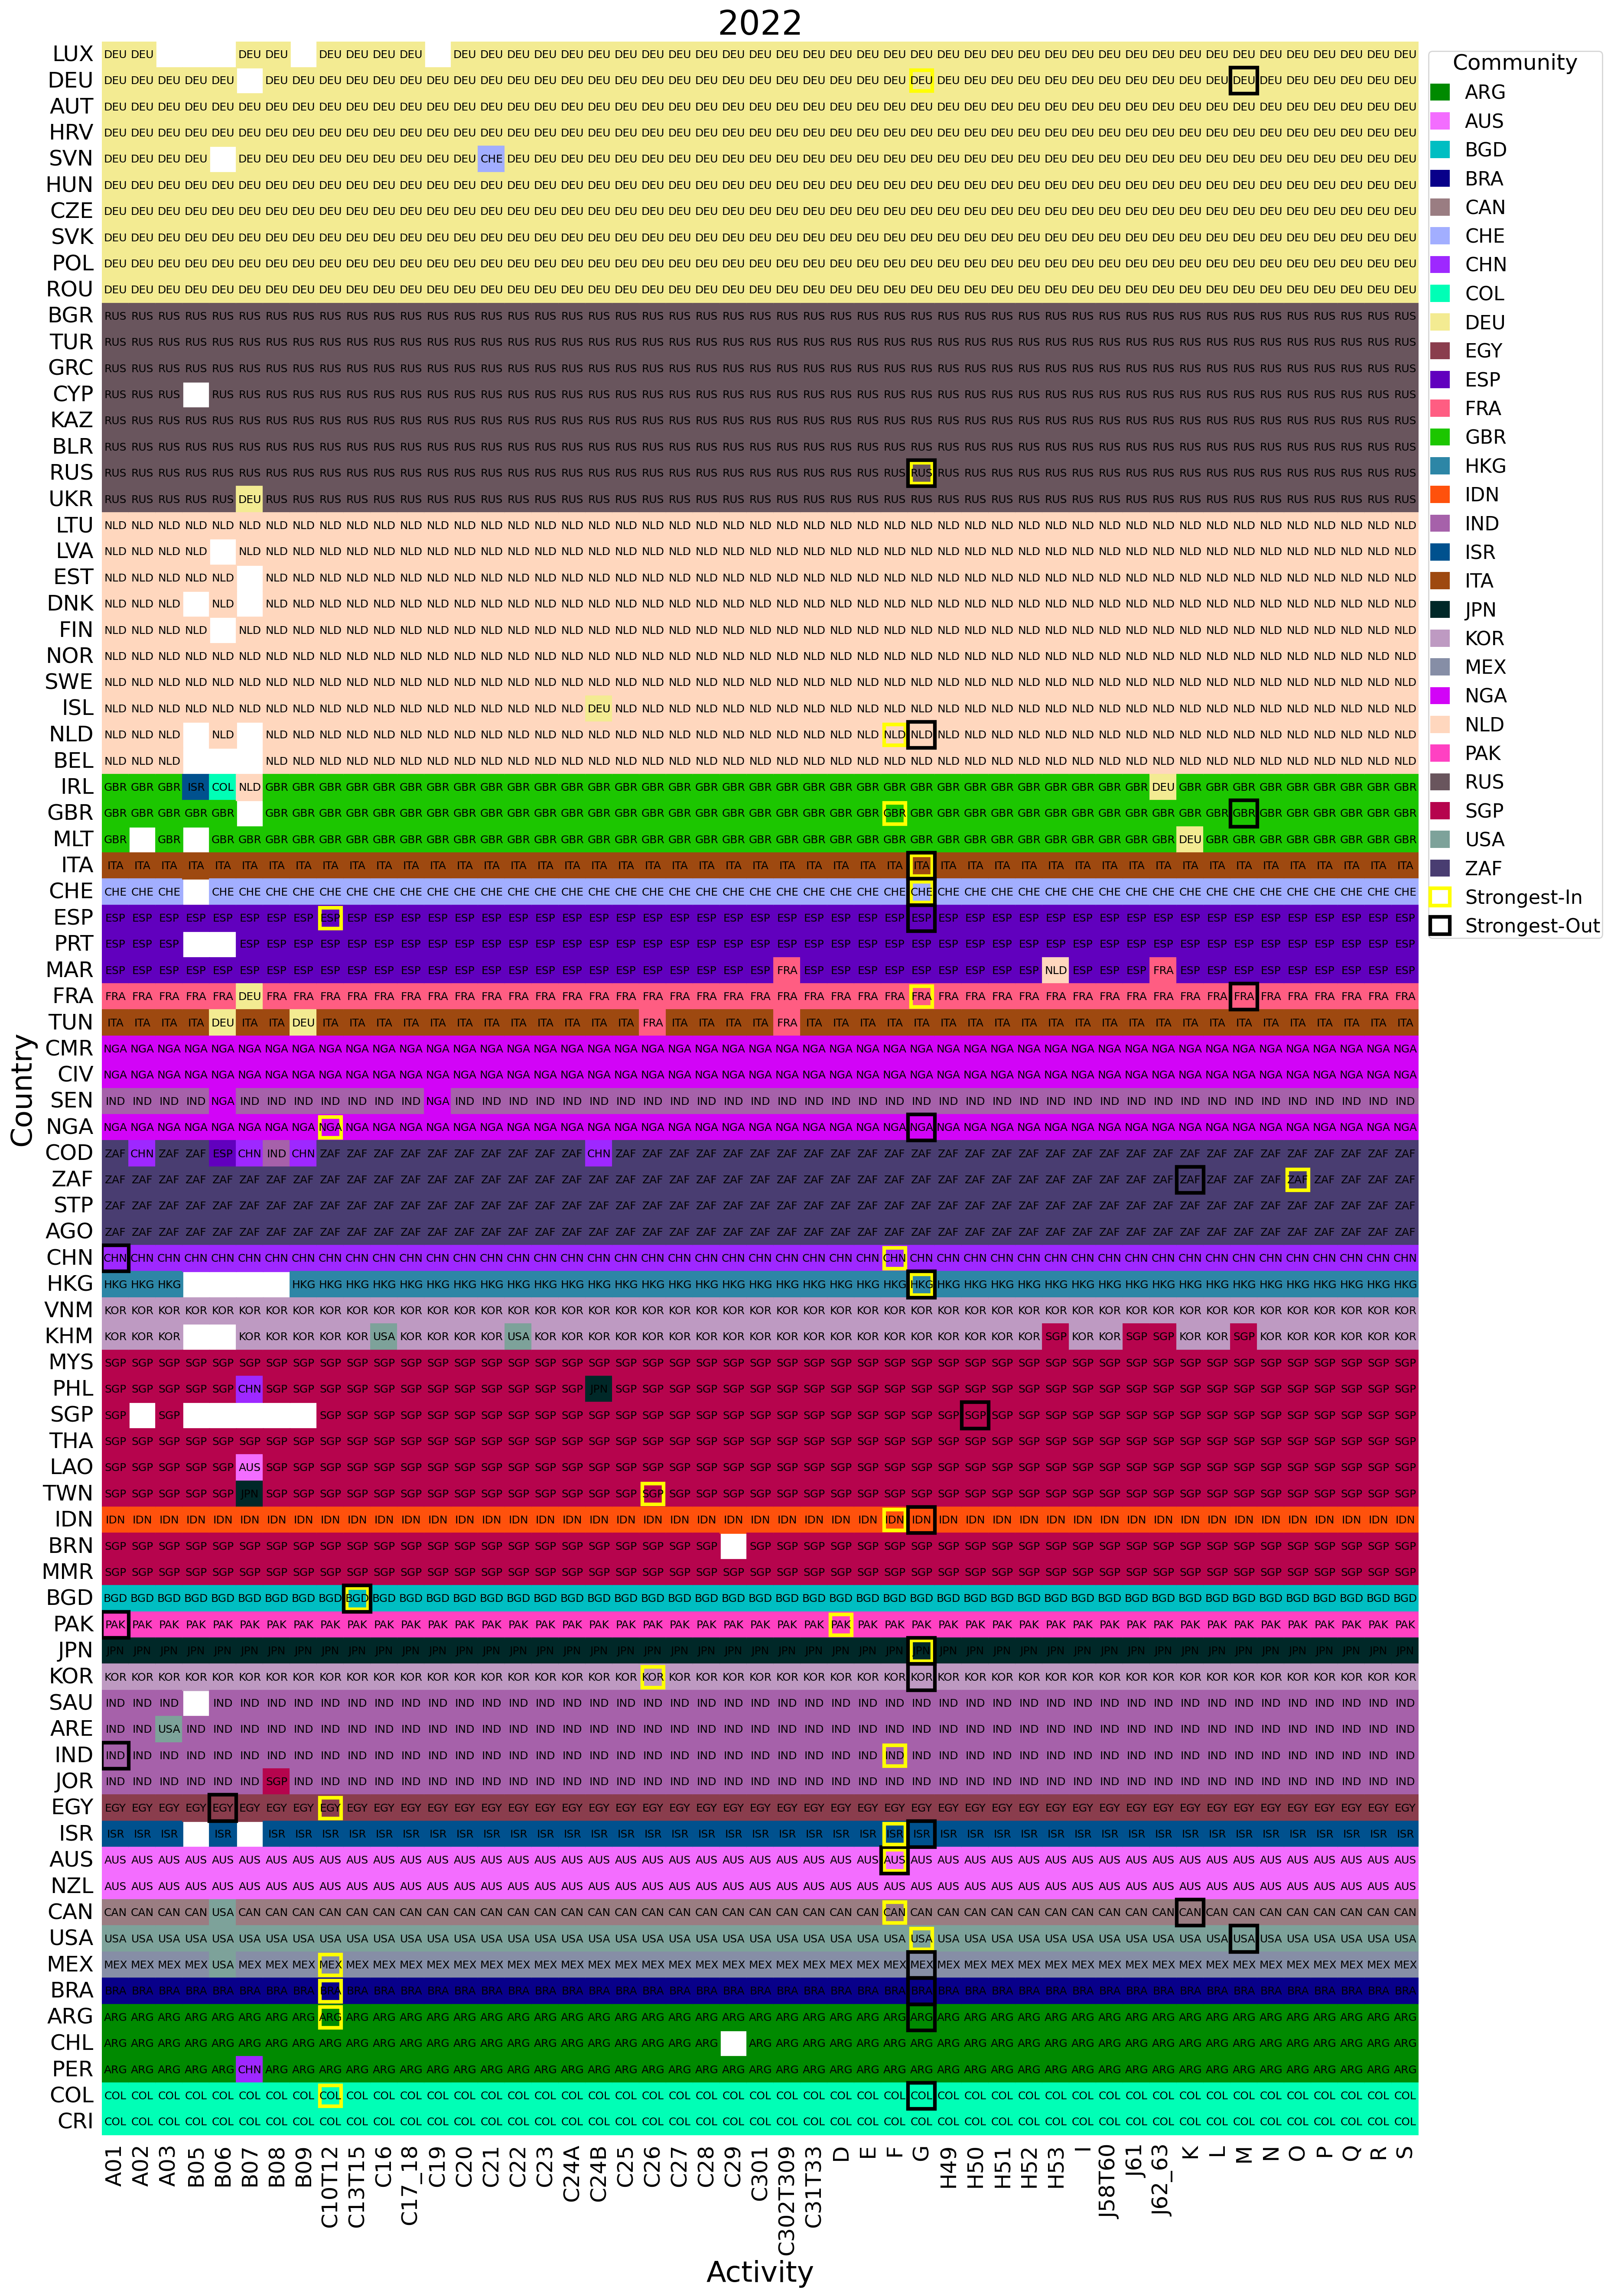
\includegraphics[width=\linewidth]{2022_communities.png}
	\caption{Resultados de la detección de comunidades en 2022.}
	\label{Fig_2022_comunidades}
\end{figure}
	}
	%{
	%\graphicspath{
	%		{../analysis_normalized/images/communities_membership/}
	%	}
	%	\chapter{}\label{Apendice4}

\begin{figure}[H]
	\centering
	
\includegraphics[width=\linewidth]{AGO.png}
	\caption{Cantidad de vértices por año en la comunidad AGO (Angola).}
	\label{AGO_timeline}
\end{figure}

\begin{figure}[H]
	\centering
	
\includegraphics[width=\linewidth]{ARE.png}
		\caption{Cantidad de vértices por año en la comunidad ARE (Emiratos Árabes Unidos).}
	\label{ARE_timeline}
\end{figure}

\begin{figure}[H]
	\centering
	
\includegraphics[width=\linewidth]{ARG.png}
	\caption{Cantidad de vértices por año en la comunidad ARG (Argentina).}
	\label{ARG_timeline}
\end{figure}

\begin{figure}[H]
	\centering
	
\includegraphics[width=\linewidth]{AUS.png}
	\caption{Cantidad de vértices por año en la comunidad AUS (Australia).}
	\label{AUS_timeline}
\end{figure}
	%}
	\end{appendices}
	
    \printbibliography[heading=bibintoc, title={Referencias bibliográficas}]
	\backmatter
	
	
\end{document}